\documentclass[twocolumn,twocolappendix]{openjournal}

\usepackage[T1]{fontenc}
\usepackage{graphicx}
\usepackage{amsmath,amssymb}
\usepackage{hyperref}
\usepackage{array}

\newcolumntype{P}[1]{>{\raggedright\arraybackslash}p{#1}}
\usepackage{booktabs}

%% ★★★ v4.11: SUPPRESS THE CLASS'S PREPRINT VERSION STAMP (referee 2, first
%% minor).  `openjournal.cls` sets `\submitted{Version \today}` and then
%% `\journalinfo{\@submitted}`, so the line is typeset twice -- once as the
%% title-page slug and once in the journal-info header -- and it was the
%% first thing on page 1.  The build pins SOURCE_DATE_EPOCH so that the
%% figures and the PDF are byte-identical run to run, which means `\today`
%% reads "January 1, 2020" and would read that for ever.
%%
%% The date is therefore NOT unfrozen: a reproducible build is worth more
%% than a date, and a date that must never change should not be printed at
%% all.  A journal submission does not want a preprint version stamp
%% either.  Both are emptied here rather than in the class, which is a
%% third-party template the journal may replace.  `abswords.py` and the
%% LaTeX-log gate both read page 1, so a regression shows up there.
\submitted{}
\journalinfo{}
% suppress the class's end-of-document template advertisement;
% delete this block to restore it
\makeatletter
\renewenvironment{bottompar}{\setbox\z@\vbox\bgroup}{\egroup}
\makeatother

% ---------------------------------------------------------------
% \pv{\Macro} -- print a probability with its relational symbol.
% Generated p-value macros are of two kinds: an ordinary value such as
% 0.186, and a bound such as <10^{-4} for a probability too small for the
% ensemble to resolve. Writing "$p=\Macro$" at the use site is right for
% the first and produces "p =< 10^-4" for the second; writing "$p\Macro$"
% is right for the second and produces "p0.186" for the first. Both
% mistakes were in the manuscript. The relation therefore belongs with
% the value, decided once, here: \pv inspects the first token of the
% expanded macro and supplies "=" unless the value already carries its
% own relational symbol.
\makeatletter
\def\@pvlt{<}\def\@pvgt{>}\def\@pveq{=}
\def\@pvfirst#1#2\@nil{%
  \def\@pvA{#1}%
  \ifx\@pvA\@pvlt <#2%
  \else\ifx\@pvA\@pvgt >#2%
  \else\ifx\@pvA\@pveq =#2%
  \else =#1#2\fi\fi\fi}
\DeclareRobustCommand{\pv}[1]{p\,\expandafter\@pvfirst#1\@nil}
\makeatother
% ---------------------------------------------------------------
% \rankstatus -- the status of the star-versus-control rank, in ONE
% formulation used verbatim wherever the question arises (referee 1, item 1).
% Earlier versions stated this in several incompatible ways: the main text
% denied exchangeability while Appendix A asserted that star and controls
% "remain exchangeable in signal-to-noise ratio", and a table caption called
% the ensemble a "calibrated screen".  A macro makes the use sites identical
% by construction rather than by proof-reading.
\DeclareRobustCommand{\rankstatus}{The star-versus-control rank is an
empirically useful way of deciding which crossing to examine first, but the
stellar and control positions are not demonstrably exchangeable under the
null. The rank therefore has no calibrated per-window false-alarm probability
and is not used as evidence for detection.}
% ---------------------------------------------------------------
\shorttitle{An ALMA Archival Technosignature Search within 40\,pc}
\shortauthors{White \& Dey}

% GENERATED by make_numbers.py -- do not edit by hand.
% Every survey quantity in the manuscript is defined here, once,
% from survey_stats.json / occurrence_v328.json / nullcal.json.
\newcommand{\NCensus}{168}
\newcommand{\NStars}{89}
\newcommand{\NSystems}{82}
\newcommand{\NStarBands}{112}
\newcommand{\NEB}{404}
\newcommand{\NExtracted}{1721}
\newcommand{\NDup}{45}
\newcommand{\NDefect}{13}
\newcommand{\NWithheld}{12}
\newcommand{\NWindows}{1651}
\newcommand{\NFine}{402}
\newcommand{\NCoarse}{1249}
\newcommand{\DistMin}{1.30}
\newcommand{\DistMax}{39.63}
\newcommand{\UnionGHz}{118.1}
\newcommand{\UnionIntervals}{46}
\newcommand{\UnionLo}{89.6}
\newcommand{\UnionHi}{873.1}
\newcommand{\ExposureSGHz}{6.8\times10^{6}}
\newcommand{\EirpMin}{1.6\times10^{13}}
\newcommand{\EirpMax}{2.8\times10^{17}}
\newcommand{\EirpMedian}{7.1\times10^{14}}
\newcommand{\SminMin}{0.41}
\newcommand{\SminMax}{1.31}
\newcommand{\SminMedian}{9.9}
\newcommand{\ChanMedianMHz}{15.625}
\newcommand{\NHits}{56}
\newcommand{\NSpatial}{12}
\newcommand{\NSpatialOld}{18}
\newcommand{\NLineAttrib}{11}
\newcommand{\NUnattrib}{1}
\newcommand{\NCandidates}{0}
\newcommand{\NCtrl}{512}
\newcommand{\RankFloor}{513}
\newcommand{\ExpFlags}{3.22}
\newcommand{\NRankFirst}{14}
\newcommand{\RateRankFirst}{0.8}
\newcommand{\RateRankFirstOld}{8.8}
\newcommand{\NRankFirstOld}{146}
\newcommand{\TrialCells}{1.32\times10^{8}}
\newcommand{\NPseudo}{220\,672}
\newcommand{\PseudoKSp}{0.37}
\newcommand{\PseudoMean}{0.5010}
\newcommand{\StarPseudoP}{0.38}
\newcommand{\OccMeasured}{5.8}
\newcommand{\OccMeasuredRound}{6}
\newcommand{\OccUnit}{3.4}
\newcommand{\OccUniform}{8.2}
\newcommand{\OccDhalf}{7.7}
\newcommand{\OccDtenth}{19}
\newcommand{\NOccSystems}{65}
\newcommand{\NOccSystemsUnit}{86}
\newcommand{\IntGainSpan}{16}
\newcommand{\FineOnsrcMedian}{2177}
\newcommand{\CalibOnsrc}{1506}
\newcommand{\CalibGainRatio}{1.2}
\newcommand{\SbrN}{14}
\newcommand{\SbrPobs}{1.7\times10^{-3}}
\newcommand{\SbrAstro}{3}
\newcommand{\SbrResid}{2}
\newcommand{\SbrResidP}{0.21}
\newcommand{\OnsrcMin}{21}
\newcommand{\OnsrcMax}{5274}
\newcommand{\MasonRatio}{1250}
\newcommand{\OnsrcMedian}{2087}
\newcommand{\DutyHalf}{7.7}
\newcommand{\DutyTenth}{19}
\newcommand{\DutyHalfUnit}{4.5}
\newcommand{\NMultiEpoch}{54}
\newcommand{\AuPct}{92.1}
\newcommand{\AuNge}{34}
\newcommand{\AuFrac}{7.9}
\newcommand{\AuP}{0.081}
\newcommand{\CtrlMed}{4.56}
\newcommand{\CtrlPninety}{5.85}
\newcommand{\NNonBP}{416}
\newcommand{\NBPWindows}{15}
\newcommand{\NDwellTrials}{3\,888}
\newcommand{\NDwellWin}{12}
\newcommand{\DwellCoarseOne}{100}
\newcommand{\DwellCoarseQ}{100}
\newcommand{\DwellCoarseT}{83}
\newcommand{\DwellFineOne}{100}
\newcommand{\DwellFineQ}{91}
\newcommand{\DwellFineT}{71}
\newcommand{\RecThresh}{42}
\newcommand{\RecThreshHi}{16}
\newcommand{\RecThreshLo}{14}
\newcommand{\RecTwice}{83}
\newcommand{\NTrials}{1200}
\newcommand{\PctBandsSixSeven}{91}

% survey_numbers_round8.tex -- generated by round8_calc.py
% from frozen_export_v3.31.json + occurrence_v328.json +
% dwell_campaign_trials_v3.32.csv (v3.31/v3.32 freezes).
% class widths / eta on frozen classes, EB reconciliation, f95
% ICC sensitivity, flag effect sizes, defect localisation,
% dwell-campaign criterion cross-check; referee round 8.

\newcommand{\ChanAMinKHz}{15.259}
\newcommand{\ChanAMaxKHz}{1953.125}
\newcommand{\ChanAMedKHz}{488.3}
\newcommand{\ChanAModeKHz}{488.3}
\newcommand{\ChanAModePct}{60}
\newcommand{\ChanBMinMHz}{7.812}
\newcommand{\ChanBMaxMHz}{31.25}
\newcommand{\ChanBMedMHz}{15.625}
\newcommand{\ChanBModeMHz}{15.625}
\newcommand{\ChanBModeN}{1209}
\newcommand{\ChanGapFac}{4.0}
\newcommand{\ChanStraddleKHz}{1953.125}
\newcommand{\EtaStraddle}{1.46}
\newcommand{\EtaAmin}{0.17}
\newcommand{\EtaAmed}{14.9}
\newcommand{\EtaAmax}{422}
\newcommand{\EtaAltOne}{13}
\newcommand{\EtaBmin}{0.004}
\newcommand{\EtaBmed}{0.51}
\newcommand{\EtaBmax}{1.35}
\newcommand{\EtaBgeOne}{38}
\newcommand{\EtaBgeOneMax}{1.35}
\newcommand{\DgridA}{0.26}
\newcommand{\DgridB}{0.29}
\newcommand{\EbsRetained}{404}
\newcommand{\EbsRankAll}{407}
\newcommand{\EbsExtraN}{3}
\newcommand{\EffEbsFine}{252}
\newcommand{\EffKbar}{1.60}
\newcommand{\EffDeff}{1.14}
\newcommand{\EffSumC}{49.8}
\newcommand{\EffFIccPct}{6.6}
\newcommand{\NFlagWin}{12}
\newcommand{\NFlagSys}{4}
\newcommand{\NFlagBpic}{9}
\newcommand{\NFlagOther}{3}
\newcommand{\DefectNoSib}{1}
\newcommand{\DefectOnsrcLo}{12}
\newcommand{\DefectOnsrcHi}{2842}
\newcommand{\DefectRmsLoSci}{4.5\times10^{-4}}
\newcommand{\DefectRmsHiSci}{14.3\times10^{-4}}
\newcommand{\DefectSibFacLo}{388}
\newcommand{\DefectSibFacHi}{743}
\newcommand{\DefectBandSix}{7}
\newcommand{\DefectBandSeven}{6}
\newcommand{\DefectNStars}{8}
\newcommand{\XcheckN}{3888}
\newcommand{\XcheckAgree}{3888}
\newcommand{\XcheckMismatch}{0}
\newcommand{\XcheckTrueMin}{5.04}
\newcommand{\XcheckFalseMax}{5.00}
\newcommand{\XcheckWin}{12}
% retired by retire_macros.py (unreferenced): BandWinEight, BandWinFive, BandWinFour, BandWinNine, BandWinSeven, BandWinSix, BandWinTen, BandWinThree, MarginBpicSix, MarginBpicThree, MarginCp, MarginHd, ZetaBpicSix, ZetaBpicThree, ZetaCp, ZetaHd

% survey_numbers_round9.tex -- generated by round9_calc.py
% from frozen_export_v3.31.json; mask-union framing derived
% from the generated Table tab:maskband (4.96 GHz all-species
% merged Union); referee round 9 (R4-B concentration, R3-8
% mask framing, R3-3 CP-72 2713 feature rows).

\newcommand{\ConcThreeNames}{BD$+$05~1668, Proxima Cen and HD~33793}
\newcommand{\ConcThreeWin}{285}
\newcommand{\ConcThreePct}{17.3}
\newcommand{\ConcThreeSys}{3}
\newcommand{\CpTwoFreqGHz}{345.1152}
\newcommand{\CpTwoTstar}{5.81}
\newcommand{\CpTwoRingMax}{5.68}
\newcommand{\CpTwoMargin}{0.13}
\newcommand{\CpTwoLineOffKms}{-1326}
\newcommand{\CpTwoNdrift}{129}
\newcommand{\CpTwoDriftkHzs}{4.14}
\newcommand{\CpTwoBwGHz}{1.73}
\newcommand{\CpTwoOnsrcS}{2994}

%% GENERATED by round10_calc.py -- do not hand-edit.
\newcommand{\CompWin}{12}
\newcommand{\CompTgt}{11}
\newcommand{\CompBands}{3, 6 and~7}
\newcommand{\CompNintLo}{21}
\newcommand{\CompNintHi}{1\,314}
\newcommand{\CompNintFactor}{63}
\newcommand{\CompFiftyN}{6}
\newcommand{\CompFiftyLo}{5.3}
\newcommand{\CompFiftyHi}{8.3}
\newcommand{\CompFiftyMed}{6.2}
\newcommand{\CompSatN}{6}
\newcommand{\CompSatMin}{3.4}
\newcommand{\CompSatRec}{97}
\newcommand{\OccAll}{4.1}
\newcommand{\NOccAll}{87}
\newcommand{\OccAllDhalf}{5.5}
\newcommand{\OccAllDtenth}{14}
\newcommand{\OccAllFifteen}{8.8}
\newcommand{\NOccAllFifteen}{75}
\newcommand{\OccAllSeventeen}{3.5}
\newcommand{\NOccAllSeventeen}{87}

%% GENERATED by round10_calc.py (v3.41 block) -- do not hand-edit.
\newcommand{\GrossBwGHz}{2828.1}
\newcommand{\GaussCross}{37.8}
\newcommand{\PgeFourPct}{40.2}
\newcommand{\ExpNonBP}{3.12}
\newcommand{\PgeOneNonBPPct}{96}
\newcommand{\FlagPairs}{5}
\newcommand{\FluxBpicThree}{76}
\newcommand{\FluxBpicSix}{78}
\newcommand{\FluxHdFour}{0.82}
\newcommand{\FluxCpSeven}{12}
\newcommand{\FluxRatioBpic}{1.0}
\newcommand{\MaskRestRoundMHz}{1}
\newcommand{\CatCOoneGHz}{115.271000}
\newcommand{\LabCOoneGHz}{115.271202}
\newcommand{\CatCOerrMHz}{0.202}
\newcommand{\CatCOerrKms}{0.53}
\newcommand{\CatWorstKms}{1.3}
\newcommand{\VsysBpic}{+20.0}
\newcommand{\VsysBpicErr}{0.7}
\newcommand{\DnuBpicCoarse}{-9.62}
\newcommand{\DvBpicCoarse}{-12.51}
\newcommand{\StelBpicThree}{-0.39}
\newcommand{\StelBpicSix}{-0.29}
\newcommand{\StelBpicCoarse}{-0.14}
\newcommand{\BpicSpreadKms}{0.2}
\newcommand{\BpicPairSepKms}{0.09}
\newcommand{\BpicMaxAbsStel}{0.39}
\newcommand{\BpicMaskPct}{0.8}
% retired by retire_macros.py (unreferenced): BaryBpicCoarse, BaryBpicSix, BaryBpicThree, DnuBpicSix, DnuBpicThree, DnuCpSeven, DnuHdFour, DvBpicSix, DvBpicThree, DvCpSeven, DvHdFour, FcenBpicSix, FcenBpicThree, FcenCpSeven, FcenHdFour, FobsBpicSix, FobsBpicThree, FobsCpSeven, FobsHdFour

%% GENERATED by v342_calc.py -- do not hand-edit.
\newcommand{\RingSeed}{20260825}
\newcommand{\RingNProbe}{512}
\newcommand{\RingNSrc}{135}
\newcommand{\RingInFrac}{0.14}
\newcommand{\RingOutFrac}{0.78}
\newcommand{\RingCheckFrac}{0.06}
\newcommand{\RingGainIn}{0.95}
\newcommand{\RingGainOut}{0.19}
\newcommand{\RingGainMean}{0.47}
\newcommand{\RingGainInTrue}{0.98}
\newcommand{\RingGainOutTrue}{0.51}
\newcommand{\RingPbCoef}{1.13}
\newcommand{\RingPbCoefCode}{1.22}
\newcommand{\RingThetaMin}{7.2}
\newcommand{\RingThetaMax}{69.5}
\newcommand{\RingRinMin}{1.0}
\newcommand{\RingRinMax}{9.7}
\newcommand{\RingRoutMin}{5.6}
\newcommand{\RingRoutMax}{54.2}
\newcommand{\RingRhoCO}{0.05}
\newcommand{\RingRhoCOexp}{-1}
\newcommand{\RingRhoNull}{0.002}
\newcommand{\RingRhoNullN}{1187}
\newcommand{\RingRhoNullLo}{-0.10}
\newcommand{\RingRhoNullHi}{0.10}
\newcommand{\RingRhoBoundPct}{10}
\newcommand{\HdThirteenOffset}{15.9}
\newcommand{\HdThirteenOffsetPB}{0.55}
\newcommand{\HdThirteenTopLo}{11.4}
\newcommand{\HdThirteenTopHi}{22.2}
\newcommand{\HdThirteenRingMed}{15.9}
\newcommand{\HdThirteenRingMax}{10.8}
\newcommand{\HdThirteenStar}{4.4}
\newcommand{\MaskNTransOld}{15}
\newcommand{\MaskNTransNew}{17}
\newcommand{\MaskNSpecOld}{9}
\newcommand{\MaskNSpecNew}{11}
\newcommand{\MaskCIGHz}{492.160651}
\newcommand{\MaskHthirtyGHz}{231.900928}
\newcommand{\MaskVWidth}{50}
\newcommand{\MaskRoundWorstKms}{1.59}
\newcommand{\PeakFreqMatched}{283}
\newcommand{\MaskFrameChained}{4}
\newcommand{\MaskFrameTotal}{12}
\newcommand{\MaskNewCoinc}{0}
\newcommand{\MaskLostOldGHz}{0.64}
\newcommand{\MaskLostNewGHz}{0.88}
\newcommand{\MaskExtraGHz}{0.24}
\newcommand{\MaskExtraPct}{0.2}
\newcommand{\NCrossFreq}{51}
\newcommand{\HanBest}{0.50}
\newcommand{\HanWorst}{0.42}
\newcommand{\HanMed}{0.48}
\newcommand{\HanFacBest}{2.00}
\newcommand{\HanFacWorst}{2.36}
\newcommand{\HanFacMed}{2.08}
\newcommand{\HanFacAvgLo}{1.18}
\newcommand{\HanFacAvgHi}{1.96}
\newcommand{\HanFacAvgMed}{1.33}
\newcommand{\NNoArchResBands}{none}
\newcommand{\NNoArchRes}{0}
\newcommand{\HanArchHi}{2.000}
\newcommand{\HanArchLo}{1.156}
\newcommand{\HanArchNHi}{1505}
\newcommand{\HanArchNLo}{145}
\newcommand{\HanNByN}{$n=1$: 1505, $n=2$: 145, $n=4$: 1}
\newcommand{\HanNFour}{1}
\newcommand{\HanFwhmFour}{1.0143}
\newcommand{\HanFacFourMed}{1.06}
\newcommand{\HanFacFourLo}{0.98}
\newcommand{\HanFacFourHi}{1.90}
\newcommand{\EirpMinA}{2.2\times10^{13}}
\newcommand{\EirpMaxA}{6.9\times10^{16}}
\newcommand{\ChanLoA}{15.3}
\newcommand{\ChanHiA}{1953}
\newcommand{\NWinA}{402}
\newcommand{\NWinB}{1249}
\newcommand{\PctCoarse}{76}
\newcommand{\AsymExpectPct}{20.9}
\newcommand{\PctFine}{24}
\newcommand{\EtaAltOneNow}{13}
\newcommand{\EtaBgeOneNow}{38}
\newcommand{\AmaxMin}{3.6}
\newcommand{\AmaxMax}{4.0}
\newcommand{\CaseDetCoarseNow}{1}
\newcommand{\CaseDetCoarseTwoNow}{4}
\newcommand{\CaseDetFineNow}{10}
\newcommand{\CaseDetDwellNow}{28}
\newcommand{\NSysInTwentyNow}{41}
\newcommand{\NStarBelowAreciboNow}{1}
\newcommand{\NEffArecibo}{0}
\newcommand{\NEffTwiceArecibo}{1}
\newcommand{\DeepestEffSci}{3.4\times10^{13}}
\newcommand{\TuNCatCov}{1637}
\newcommand{\TuNCatUncov}{14}
\newcommand{\TuNCatDupExtract}{67}
\newcommand{\TuNCatAmbig}{2}
\newcommand{\DispoNAttrComputed}{16}
\newcommand{\DispoNAttrRanked}{10}
\newcommand{\DispoNAttrBlank}{6}
\newcommand{\DispoNHandEntries}{12}
\newcommand{\DispoNHandOldEntries}{5}
\newcommand{\DispoNShipped}{12}
\newcommand{\DispoOldKeyReach}{4}
\newcommand{\DispoNMislabel}{2}
\newcommand{\DispoMislabelMinKms}{3794}
\newcommand{\DispoMislabelMaxKms}{3898}
\newcommand{\DispoHalfKms}{50}
\newcommand{\NStarsReleased}{89}
\newcommand{\NCatRows}{1651}
\newcommand{\NCatCols}{62}
\newcommand{\NCatFlagGlobal}{12}
\newcommand{\NCatFlagLocal}{11}
% retired by retire_macros.py (unreferenced): ChanHiB, ChanLoB, ChanMedA, ChanMedB, EirpHanMaxA, EirpHanMaxB, EirpHanMedA, EirpHanMedB, EirpHanMinA, EirpHanMinB, EirpMaxB, EirpMedA, EirpMedB, EirpMinB

% Generated by v343_calc.py -- do not edit by hand.
\newcommand{\NSmearNoValue}{1200}
\newcommand{\NSmearLo}{9}
\newcommand{\NSmearWorst}{5}
\newcommand{\SmearWorstPenLo}{1.65}
\newcommand{\SmearWorstPenHi}{1.74}
\newcommand{\SmearWorstChanKHz}{15.3}
\newcommand{\NSmearFlagged}{2}
\newcommand{\NSmearOk}{442}
\newcommand{\SmearList}{HIP~10679 Band~6 (0.574, $\times$1.74), $\beta$~Pic Band~6 (0.574, $\times$1.74), HD~172555 Band~6 (0.574, $\times$1.74), HIP~10679 Band~6 (0.606, $\times$1.65), HD~172555 Band~6 (0.606, $\times$1.65), $\eta$~Crv Band~8 (0.865, $\times$1.16), $\eta$~Crv Band~7 (0.932, $\times$1.07), HD~48370 Band~6 (0.979, $\times$1.02) and CP$-$72~2713 Band~6 (0.979, $\times$1.02)}
\newcommand{\PbMedian}{1.00002}
\newcommand{\PbPninety}{1.002}
\newcommand{\NPbAboveTwoPct}{83}
\newcommand{\NPbAboveTenPct}{34}
\newcommand{\PbMaxStar}{LP~736-15}
\newcommand{\PbMaxBand}{7}
\newcommand{\PbMax}{1.81}
\newcommand{\PbMaxRoverTheta}{0.46}
\newcommand{\PbMaxRoverFwhm}{0.50}
\newcommand{\NSirWin}{12}
\newcommand{\PbSirLoPct}{3.6}
\newcommand{\PbSirHiPct}{18.6}
\newcommand{\PbSirRoverThetaLo}{0.11}
\newcommand{\PbSirRoverThetaHi}{0.25}
\newcommand{\NPbTierStars}{5}
\newcommand{\CtrlMaxSurveyMax}{19.7}
\newcommand{\CtrlMaxSurveySecond}{19.5}
\newcommand{\BpicNFlagThree}{5}
\newcommand{\BpicNFlagSix}{4}
\newcommand{\BpicBThreeTsym}{30.76}
\newcommand{\BpicBSixTsym}{11.68}
\newcommand{\BpicAddOneDen}{1652}
\newcommand{\BpicCoRingMax}{18.3}
\newcommand{\BpicCoRingRank}{7}
\newcommand{\SurvFreqLo}{90}
\newcommand{\SurvFreqHi}{873}
\newcommand{\NWinBandThree}{112}
\newcommand{\SurvFreqLoA}{114}
\newcommand{\SurvFreqHiA}{873}
\newcommand{\UnionBandThree}{20.6}
\newcommand{\UnionBandsFourEight}{97.5}
\newcommand{\UnionHiBandLabel}{Bands~4--10}
\newcommand{\UnionHiLoGHz}{142}
\newcommand{\UnionHiHiGHz}{873}
\newcommand{\GrossOverUnion}{23.9}
\newcommand{\MedWin}{65}
\newcommand{\MedWinSplit}{130}
\newcommand{\MedWinFineLo}{65}
\newcommand{\MedWinFineHi}{74}
\newcommand{\MedWinCoarseLo}{30}
\newcommand{\MedWinCoarseHi}{59}
\newcommand{\NWinFullWidth}{133}
\newcommand{\MedWinCeilFineMHz}{32}
\newcommand{\MedWinCeilCoarseGHz}{0.9}
\newcommand{\ChanFineKHz}{488}
\newcommand{\ChanCoarseMHz}{15.62}
\newcommand{\CellsTotal}{$1.32\times10^{8}$}
\newcommand{\CellsWinMed}{468}
\newcommand{\CellsWinMax}{6\,869\,740}
\newcommand{\CellsWinMin}{177}
\newcommand{\CellExpect}{37.8}
\newcommand{\NHitWindowsNoPk}{42}
\newcommand{\CellsObserved}{219}
\newcommand{\CellsObsFlagged}{206}
\newcommand{\CellsObsRest}{13}
\newcommand{\NHitWindows}{56}
\newcommand{\NHitWindowsRest}{44}
\newcommand{\CellsRestOverExpect}{0.3}
\newcommand{\NCrossWin}{51}
\newcommand{\NCrossNoFreq}{5}
\newcommand{\EdgeFracMin}{0.010}
\newcommand{\EdgeChanMin}{35}
\newcommand{\EdgeFracSecond}{0.024}
\newcommand{\EdgeStarSecond}{HD~48370}
\newcommand{\EdgeChanSecond}{92}
\newcommand{\EdgeTwoFlagPct}{1.6}
\newcommand{\EdgeFracBpicLo}{0.48}
\newcommand{\EdgeFracBpicHi}{0.50}
\newcommand{\NPeakOuterThree}{32}
\newcommand{\NPeakRows}{490}
\newcommand{\AcaDiamRatio}{1.71}
\newcommand{\NEbSevenM}{265}
\newcommand{\NWinSevenM}{1054}
\newcommand{\PctWinSevenM}{64}
\newcommand{\NWinRinBelowBeam}{974}
\newcommand{\BeamMinArcsec}{0.08}
\newcommand{\BeamMaxArcsec}{6.0}
\newcommand{\BeamMedArcsec}{4.15}
\newcommand{\NeffMed}{63}
\newcommand{\NeffLo}{34}
\newcommand{\NeffHi}{$1.5\times10^{5}$}
\newcommand{\NHanKnown}{1651}
\newcommand{\NHanTwo}{1505}
\newcommand{\NHanTwoCoarse}{1217}
\newcommand{\NCoarseHanKnown}{1249}
\newcommand{\NHanOther}{146}
\newcommand{\NProgenitorEB}{656}
\newcommand{\NMousMulti}{116}
\newcommand{\NMous}{152}
\newcommand{\NWinMultiEB}{1480}
\newcommand{\PctWinMultiEB}{90}
\newcommand{\NStarMultiEB}{65}
\newcommand{\CpCatFreq}{344.269746}
\newcommand{\NCpTube}{3}
\newcommand{\CpTubeList}{the unidentified Lovas entry at $7$ ($7$) km\,s$^{-1}$, SO 8(8)-7(7) at $-12$ ($-13$) km\,s$^{-1}$, $^{34}$SO$_{2}$ 10(4,6)-10(3,7) at $45$ ($44$) km\,s$^{-1}$}
\newcommand{\CpSoFreq}{344.310612}
\newcommand{\CpSoVstar}{-12.3}
\newcommand{\CpSoEu}{87}
\newcommand{\CpSotwoEu}{89}
\newcommand{\NCrossWithCat}{19}
\newcommand{\NCrossQueried}{20}
\newcommand{\CrossCatMedian}{3}
\newcommand{\LNpCPgum}{$4.4\times10^{-3}$}
\newcommand{\LNGumRatio}{3.6}
\newcommand{\LNpCPRing}{$3.0\times10^{-3}$}
\newcommand{\LNCPRingRatio}{1.9}
\newcommand{\CpTrimPct}{4}
\newcommand{\CpEdgeInsideMHz}{92}
\newcommand{\AccelCeilLo}{3.60}
\newcommand{\AccelCeilHi}{4.00}
\newcommand{\DriftCeilLo}{12.0}
\newcommand{\DriftCeilHi}{13.3}
\newcommand{\NAccelPlanet}{56}
\newcommand{\DriftGridFineHalf}{0.26}
\newcommand{\DriftGridCoarseHalf}{0.28}
% retired by retire_macros.py (unreferenced): BpicBSixAddOne, BpicBThreeAddOne, NCtrlGeBpicBSix, NCtrlGeBpicBThree

%% GENERATED by pointing_calc.py -- do not hand-edit.
\newcommand{\NAudit}{68}
\newcommand{\NNotPointed}{60}
\newcommand{\NPointed}{8}
\newcommand{\SepMedianDeg}{1.6}
\newcommand{\SepMinArc}{250}
\newcommand{\SepMaxArc}{8\,205}
\newcommand{\SepPointedArc}{5.8}
\newcommand{\FovMaxDeg}{63}
\newcommand{\PmFastest}{5.12}
\newcommand{\PmYears}{49}

%% GENERATED by v346_calc.py -- do not hand-edit.
\newcommand{\NGaiaCensus}{17\,566}
\newcommand{\NCoveredCand}{168}
\newcommand{\NSearchedStars}{88}
\newcommand{\NTargetBandAttempt}{208}
\newcommand{\NTargetBandFail}{68}
\newcommand{\NNotPointedTB}{60}
\newcommand{\NPointedTB}{8}
\newcommand{\NNeverObsStars}{53}
\newcommand{\NCapCause}{0}
\newcommand{\NUntriedWithCal}{14}
\newcommand{\SepDeadMin}{250}
\newcommand{\SepDeadMax}{8\,205}
\newcommand{\SepDeadMed}{5\,603}
\newcommand{\SepDeadMedDeg}{1.6}
\newcommand{\SepPointedMax}{5.8}
\newcommand{\FovHalfMaxDeg}{63}
\newcommand{\PmFastestArcsecYr}{5.12}
\newcommand{\PmYearsToClose}{49}
\newcommand{\NTpOnlyTB}{20}
\newcommand{\NEphemTB}{56}
\newcommand{\NRetryAttempt}{39}
\newcommand{\NRetrySuccess}{1}
\newcommand{\NRetryFail}{38}
\newcommand{\RetrySuccessName}{AU~Mic [B9]}
\newcommand{\BpRecThreeTuneChanMax}{1.00}
\newcommand{\BpRecNBlocksBary}{4}
\newcommand{\BpRecVsysList}{+19.6, +20.2, +20.4, +20.7}
\newcommand{\BpRecVsysSpread}{0.7}
\newcommand{\BpRecVsys}{20}
\newcommand{\NEpochExtBlocks}{2}
\newcommand{\FobsBpicSixB}{230.528134}
\newcommand{\FobsBpicThreeB}{115.260644}
\newcommand{\NEpochExtSearched}{4}
\newcommand{\NGenuinelyCovered}{115}
\newcommand{\NSefdModelled}{431}
\newcommand{\SefdResidMed}{0.76}
\newcommand{\SefdResidLo}{0.59}
\newcommand{\SefdResidHi}{0.95}
\newcommand{\SefdResidMin}{0.39}
\newcommand{\SefdResidMax}{1.73}
\newcommand{\SefdResidDefLo}{-3.05}
\newcommand{\SefdResidDefHi}{-2.66}
\newcommand{\SefdResidSpreadDex}{0.36}
\newcommand{\SefdResidSpreadFac}{2.3}
\newcommand{\SefdResidGapDex}{0.04}
\newcommand{\SefdResidPctHalfDex}{98.4}
\newcommand{\SefdResidDefGapDex}{3.0}
\newcommand{\DefectArrays}{12\,m}
\newcommand{\NDefectArraySeven}{0}
\newcommand{\NDefectArrayTwelve}{6}
\newcommand{\NDefectProjects}{4}
\newcommand{\NDefectEBs}{5}
\newcommand{\DefectChanwMHz}{15.6}
\newcommand{\DefectChanwMinMHz}{15.6}
\newcommand{\NDefectWin}{6}
\newcommand{\NDefectBandSix}{3}
\newcommand{\NDefectBandSeven}{3}
\newcommand{\NDefectSibling}{6}
\newcommand{\DefectSibRatioLo}{2.9\times10^{3}}
\newcommand{\DefectSibRatioHi}{6.3\times10^{3}}
\newcommand{\StatFlagHash}{8e00f90e8f8c}
\newcommand{\StatFlagDate}{2026 August 31}
\newcommand{\StatSymHash}{0c465f2661bd}
\newcommand{\StatSymDate}{2026 September 9}
\newcommand{\StatGapDays}{9}
\newcommand{\CpCritHash}{119a68a6ab50}
\newcommand{\CpCritDate}{2026 September 11}
\newcommand{\CpCritLeadHours}{9}
\newcommand{\NCtrlFiveSigma}{3.5\times10^{6}}
\newcommand{\GrossWindowSumGHz}{717}
% retired by retire_macros.py (unreferenced): BpRecSixAllDet, BpRecSixChan, BpRecSixChanKHz, BpRecSixDet, BpRecSixDfMHz, BpRecSixDvKms, BpRecSixErrOne, BpRecSixErrTwo, BpRecSixFluxOne, BpRecSixFluxSig, BpRecSixFluxTwo, BpRecSixGapD, BpRecSixHitsList, BpRecSixHitsOne, BpRecSixHitsTwo, BpRecSixNBlocks, BpRecSixNBlocksExtra, BpRecSixNChan, BpRecSixOnsrcOne, BpRecSixOnsrcTwo, BpRecSixSpreadChan, BpRecSixSpreadMHz, BpRecSixTList, BpRecSixTone, BpRecSixTtwo, BpRecSixTuneChanList, BpRecSixTuneChanMax, BpRecThreeAllDet, BpRecThreeChan, BpRecThreeChanKHz, BpRecThreeDet, BpRecThreeDfMHz, BpRecThreeDvKms, BpRecThreeErrOne, BpRecThreeErrTwo, BpRecThreeFluxOne, BpRecThreeFluxSig, BpRecThreeFluxTwo, BpRecThreeGapD, BpRecThreeHitsList, BpRecThreeHitsOne, BpRecThreeHitsTwo, BpRecThreeNBlocks, BpRecThreeNBlocksExtra, BpRecThreeNChan, BpRecThreeOnsrcOne, BpRecThreeOnsrcTwo, BpRecThreeSpreadChan, BpRecThreeSpreadMHz, BpRecThreeTList, BpRecThreeTone, BpRecThreeTtwo, BpRecThreeTuneChanList

%% GENERATED by v347_calc.py -- do not hand-edit.
\newcommand{\BpFlagSixNUnsearched}{0}
\newcommand{\BpFlagSixNProg}{2}
\newcommand{\BpFlagSixNSearched}{2}
\newcommand{\BpRecSixRingList}{15.17, 15.08}
\newcommand{\BpRecSixRingRatio}{1.5}
\newcommand{\BpRecSixNCtrlGe}{0 and 6}
\newcommand{\BpRecSixRin}{3.82}
\newcommand{\BpRecSixRout}{21.27}
\newcommand{\BpRecSixChanwKHz}{244.14}
\newcommand{\BpRecSixClass}{A}
\newcommand{\BpRecSixResClass}{fine}
\newcommand{\BpBeltAu}{85}
\newcommand{\BpBeltArcsec}{4.3}
\newcommand{\BpDistPc}{19.6}
\newcommand{\BpWidthThreeLo}{10.8}
\newcommand{\BpWidthThreeHi}{15.2}
\newcommand{\BpWidthSixRecLo}{8.9}
\newcommand{\BpWidthSixRecHi}{10.2}
\newcommand{\BpWidthSixMHz}{1.74}
\newcommand{\BpWidthSixKms}{2.26}
\newcommand{\NCrossBpicSix}{114}
\newcommand{\BpBaselineYr}{8.4}
\newcommand{\BpSpanFirst}{2013-10-06}
\newcommand{\BpSpanLast}{2022-03-03}
\newcommand{\BpSixGapD}{25}
\newcommand{\BpThreeSessionH}{23}
\newcommand{\BpNBlocksTotal}{6}
\newcommand{\BpAllBlocksRingBelow}{yes}
\newcommand{\BpThreeRingMax}{7.34}
\newcommand{\BpThreeTmin}{14.65}
\newcommand{\BeamBpicThree}{2.71}
\newcommand{\BeamBpicSixFlag}{1.09}
\newcommand{\BeamBpicSixRec}{4.29}
\newcommand{\CpRecStartSepH}{2.05}
\newcommand{\CpRecTotalSpanH}{3.1}
\newcommand{\EirpMedWithSirius}{0.7}
\newcommand{\EirpMedNoSirius}{0.7}
\newcommand{\NSiriusWin}{12}
\newcommand{\UVCetiRms}{0.241}
\newcommand{\UVCetiEB}{A002\_X877e41\_X14c1}
\newcommand{\UVCetiFlo}{91.565}
\newcommand{\UVCetiSmin}{1.21}
\newcommand{\NUVCetiWin}{4}
\newcommand{\HanRhoOne}{0.667}
\newcommand{\HanRhoTwo}{0.167}
\newcommand{\HanSigRatio}{0.612}
\newcommand{\HanRhoOneFrac}{2/3}
\newcommand{\HanRhoTwoFrac}{1/6}
\newcommand{\FaPredFine}{5.74}
\newcommand{\FaPredCoarse}{4.47}
\newcommand{\FaPredFineCorr}{5.45}
\newcommand{\FaPredCoarseCorr}{4.10}
\newcommand{\FaOverCount}{5.3}
\newcommand{\FaExcessFine}{6}
\newcommand{\FaExcessCoarse}{8}
\newcommand{\FaShiftLo}{0.4}
\newcommand{\FaShiftHi}{0.3}
\newcommand{\ArecScaledW}{2}
\newcommand{\ArecGHz}{2.38}
\newcommand{\NCtrlCap}{512}
\newcommand{\PlxWorstPct}{2.48}
\newcommand{\NPlxOverEight}{3}
\newcommand{\PlxAdqlPct}{20}
% retired by retire_macros.py (unreferenced): BpUnitSixAvail, BpUnitSixDone, BpUnitSixExhaustive, BpUnitThreeAvail, BpUnitThreeDone, BpUnitThreeExhaustive, CtrlMedCoarse, CtrlMedFine, NMedCoarseWin, NMedFineWin

% generated by v348_calc.py -- do not edit
\newcommand{\NDiskCatStars}{80}
\newcommand{\NDebrisKwStars}{74}
\newcommand{\NDebrisKwSys}{69}
\newcommand{\NObscoreBlocks}{404}
\newcommand{\RzeroKpc}{8.15}
\newcommand{\ThetaZeroKms}{236}
\newcommand{\VlsrHdLsr}{23.9}
\newcommand{\KinDistKpc}{2.07}
\newcommand{\VlsrTwoKpc}{23.2}

%% GENERATED by recurrence_calc.py -- do not hand-edit.
\newcommand{\CpRecNInt}{495}
\newcommand{\CpRecChanwkHz}{488.28}
\newcommand{\CpRecChan}{35}
\newcommand{\CpRecOffkHz}{87.6}
\newcommand{\CpRecOffChan}{0.18}
\newcommand{\CpRecDate}{2022 October 2}
\newcommand{\CpRecUTone}{00:40}
\newcommand{\CpRecUTtwo}{02:42}
\newcommand{\CpRecGapMin}{60}
\newcommand{\CpRecStartSep}{2.0}
\newcommand{\CpRecRmsOne}{2.097}
\newcommand{\CpRecRmsTwo}{1.964}
\newcommand{\CpRecDeeperPct}{6.3}
\newcommand{\CpRecSminTwo}{9.82}
\newcommand{\CpRecExpT}{6.21}
\newcommand{\CpRecT}{3.60}
\newcommand{\CpRecCtrlMed}{4.62}
\newcommand{\CpRecCtrlMax}{5.93}
\newcommand{\CpRecWinPeak}{4.70}
\newcommand{\CpRecWinPeakGHz}{344.7648}
\newcommand{\CpRecHits}{0}
\newcommand{\CpRecCtrlMedOne}{4.63}
\newcommand{\CpRecCtrlMaxOne}{5.68}
\newcommand{\CpRecHitsOne}{2}
\newcommand{\CpRecRank}{188}
\newcommand{\CpRecRankOf}{513}
\newcommand{\CpRecRankP}{0.37}
\newcommand{\CpRecNbrMean}{3.23}
\newcommand{\CpRecNbrSd}{0.63}
\newcommand{\CpRecNbrSig}{0.6}
\newcommand{\CpRecDriftkHzs}{-2.06}
\newcommand{\CpRecSweepMHz}{7.70}
\newcommand{\CpRecSweepChan}{15.8}
\newcommand{\CpRecAccel}{1.79}
\newcommand{\CpRecFluxOne}{11.3}
\newcommand{\CpRecErrOne}{2.0}
\newcommand{\CpRecFluxTwo}{-1.0}
\newcommand{\CpRecErrTwo}{1.8}
\newcommand{\CpRecSigTwo}{-0.6}
\newcommand{\CpRecExclCond}{6.8}
\newcommand{\CpRecExclPair}{4.6}
\newcommand{\CpRecExclDmax}{1.6}
\newcommand{\CpRecNodeChan}{0.12}
\newcommand{\CpRecZeroSig}{2.02}
\newcommand{\CpRecOthA}{2.65}
\newcommand{\CpRecOthB}{2.98}
\newcommand{\CpRecOthC}{4.47}

% Generated by v344_calc.py -- do not edit by hand.
\newcommand{\ExpCrossWin}{33.2}
\newcommand{\ExpCrossWinFine}{33.0}
\newcommand{\ExpCrossWinCoarse}{0.16}
\newcommand{\CellsFineSci}{$13.12\times10^{7}$}
\newcommand{\CrossWinRatio}{1.3}
\newcommand{\CrossWinPoisson}{0.04}
\newcommand{\CellsPerCrossN}{9}
\newcommand{\CellsPerCrossExp}{1.1}
\newcommand{\CellsPerCrossObs}{1.6}
\newcommand{\CellsPerCrossRatio}{1.4}
\newcommand{\NCtrlWinObs}{455}
\newcommand{\NCtrlWinExp}{476}
\newcommand{\CtrlWinRatio}{0.96}
\newcommand{\CtrlWinAgreePct}{4}
\newcommand{\CtrlMaxRatioMed}{0.995}
\newcommand{\CtrlMaxRatioLo}{0.91}
\newcommand{\CtrlMaxRatioHi}{1.11}
\newcommand{\CtrlMaxFineObs}{5.77}
\newcommand{\CtrlMaxFinePred}{5.72}
\newcommand{\CtrlMaxCoarseObs}{4.44}
\newcommand{\CtrlMaxCoarsePred}{4.53}
\newcommand{\BaseNodeFirst}{32.7}
\newcommand{\CpNChan}{3534}
\newcommand{\BaseBlockWidth}{65.4}
\newcommand{\CpNodeDistChan}{2.3}
\newcommand{\NEbHeldOut}{77}
\newcommand{\NEbProcessedAll}{484}
\newcommand{\NEbSurveyAssigned}{407}
\newcommand{\NEbSurveyNoWindow}{3}
\newcommand{\NProgenitorEBTotal}{656}
\newcommand{\NUnsearchedEB}{252}
\newcommand{\PctEbSearched}{61.6}
\newcommand{\NStarMoreEB}{50}
\newcommand{\NStarUnsearchedEB}{29}
\newcommand{\NSysUnsearchedEB}{27}
\newcommand{\NExtraBlocksUnsearched}{135}
\newcommand{\NExtraBlocksHeldOut}{67}
\newcommand{\NSysOneEBGain}{5}
\newcommand{\NSysOneEBNoGain}{22}
\newcommand{\MaxProgEBStar}{60}
\newcommand{\MaxSearchedEBStar}{25}
\newcommand{\NSysSingleEB}{17}
\newcommand{\NSysMultiEB}{65}
\newcommand{\CpMousProg}{2}
\newcommand{\CpMousSearched}{2}
\newcommand{\CpMous}{uid://A001/X2d20/X2e25}
\newcommand{\CpEbSearched}{A002\_Xff0235\_X4a6d}
\newcommand{\CpEbUnsearched}{none remaining}
\newcommand{\CpEbSearchedGB}{49.3}
\newcommand{\CpEbUnsearchedGB}{0.0}
\newcommand{\BeltRadiusAu}{140}
\newcommand{\BeltRadiusArcsec}{3.8}
\newcommand{\CoAssumedDVkms}{4}
\newcommand{\CpRinAu}{94}
\newcommand{\CpRoutAu}{522}
\newcommand{\CpBeamSeven}{0.61}
\newcommand{\CpNantSeven}{47}
\newcommand{\CpBeamSix}{5.71}
\newcommand{\CpBeamSixAu}{210}
\newcommand{\CpNantSix}{9}
\newcommand{\CpArraySix}{7\,m}
\newcommand{\CoTwoOneLimMJy}{85}
\newcommand{\CoThreeTwoLimMJy}{8.2}
\newcommand{\CoMassLo}{1.6}
\newcommand{\CoMassHi}{2.4}
\newcommand{\CoMassEarthLo}{2.7}
\newcommand{\CoMassEarthHi}{4.0}
\newcommand{\CoTempLo}{20}
\newcommand{\CoTempHi}{50}
\newcommand{\CpFilterKms}{28}
\newcommand{\CpFilterMHz}{32}
\newcommand{\NCpTubeIdent}{2}
\newcommand{\NCpTubeUnid}{1}
\newcommand{\CpUnidQn}{U$-$344288.4}
\newcommand{\CpUnidVstar}{+7.0}
\newcommand{\CpUnidList}{Lovas}
\newcommand{\CpVarRatio}{1.006}
\newcommand{\LNpCPstar}{$2.0\times10^{-3}$}
\newcommand{\CpSplitLo}{3.08}
\newcommand{\CpSplitHi}{5.12}
\newcommand{\CpSplitExp}{4.11}
\newcommand{\CpSplitSigma}{1.4}
\newcommand{\CpNInt}{495}
\newcommand{\CpContMjy}{0.07}
\newcommand{\CpContErrMjy}{0.06}
\newcommand{\CpContThreeSig}{0.17}
\newcommand{\AuMicFlareLo}{6.1}
\newcommand{\AuMicFlareHi}{16.8}
\newcommand{\CpBandpassEps}{70}
\newcommand{\AcaAnnGain}{0.75}
\newcommand{\AcaAnnFracLo}{0.08}
\newcommand{\AcaAnnFracHi}{0.46}
\newcommand{\NPbHiTwelve}{48}
\newcommand{\NPbHiSeven}{35}
\newcommand{\AcaCorrShown}{1.05}
\newcommand{\AcaCorrTrue}{1.017}
\newcommand{\HdBeamArcsec}{5.55}
\newcommand{\HdCoOffsetBeams}{2.9}
\newcommand{\HdCoTopBeamsLo}{2.1}
\newcommand{\HdCoTopBeamsHi}{4.0}
\newcommand{\NDistinctDatasets}{1616}
\newcommand{\CompoundWorst}{4.6}
\newcommand{\UnionBandThreeFrac}{0.18}
\newcommand{\PctSampleOfCensus}{0.51}
\newcommand{\PctSysOfCensus}{0.47}

%% Generated by localnull_calc.py from v342_local_null.json.
%% Second-stage local null for the four stage-1 flagged windows
%% (referee A item 5).  DO NOT EDIT BY HAND.
\newcommand{\LNLagOne}{0.65}
\newcommand{\LNNRetained}{8}
\newcommand{\LNNWindows}{4}
% retired by retire_macros.py (unreferenced): LNCPAgreeFac, LNCPBootPct, LNCPKS, LNCPNullMax, LNCPNullMed, LNCPRatio, LNCPRealMed, LNCPRecal, LNCPSubMax, LNCPSubN, LNDrawsMax, LNDrawsMin, LNHDKSstat, LNHDNullMax, LNHDNullMed, LNHDPctAbove, LNHDRealMed, LNHDnAbove, LNNBootGEV, LNNCtrlClear, LNNFirstStage, LNTailDex, LNTstarMaxDiff, LNValidHi, LNValidLo, LNnExceedCP, LNpBpicSix, LNpBpicSixGEV, LNpBpicThree, LNpBpicThreeGEV, LNpCP, LNpCPgev, LNpCPgevHi, LNpCPgevLo, LNpHDgev, LNpHDgevHi, LNpHDgevLo

%% Generated by v350_calc.py -- do not edit by hand.
\newcommand{\BonfRankRatio}{64}
\newcommand{\RankFloorVal}{1.95\times10^{-3}}
\newcommand{\BonfNWinCheck}{1651}
\newcommand{\BonfScaleHere}{3.028e-05}
\newcommand{\CalNWindows}{3}
\newcommand{\CalBand}{6}
\newcommand{\CalChanKHz}{488}
\newcommand{\CalOnSrcS}{1905}
\newcommand{\CalNDrift}{62}
\newcommand{\CalNInt}{}
\newcommand{\CfgNA}{402}
\newcommand{\CfgAxesZero}{121}
\newcommand{\CfgAxesOne}{90}
\newcommand{\CfgAxesTwo}{168}
\newcommand{\CfgAxesThree}{23}
\newcommand{\CfgAxesZeroOne}{211}
\newcommand{\CfgAxesZeroOnePct}{52}
\newcommand{\CfgOffTol}{0.2}
\newcommand{\CfgChanIn}{372}
\newcommand{\CfgOnSrcIn}{315}
\newcommand{\CfgDriftIn}{235}
\newcommand{\CfgOffIn}{389}
\newcommand{\CfgBandIn}{203}
\newcommand{\CfgOffHi}{0.45}
\newcommand{\NEpsWithheld}{12}
\newcommand{\EpsEriNWin}{12}
\newcommand{\EpsEriEirpLo}{3.7\times10^{13}}
\newcommand{\EpsEriEirpHi}{1.1\times10^{15}}
\newcommand{\EpsEriPbLo}{1.0}
\newcommand{\EpsEriPbHi}{3.5}
\newcommand{\EpsEriDistPc}{3.22}
\newcommand{\EpsEriNFine}{3}
% retired by retire_macros.py (unreferenced): CfgChanHi, CfgChanLo, CfgDriftHi, CfgDriftLo, CfgOnSrcHi, CfgOnSrcLo

%% GENERATED by v351_calc.py -- do not hand-edit.
\newcommand{\EirpEffDeepest}{3.4\times10^{13}}
\newcommand{\CaseDetNomArec}{1}
\newcommand{\CaseDetNomArecTwo}{4}
\newcommand{\CaseDetEffArec}{0}
\newcommand{\CaseDetEffArecTwo}{1}
\newcommand{\AreciboW}{2.0\times10^{13}}
\newcommand{\BenchEta}{0.7}
\newcommand{\BenchEffRatio}{3.1}
\newcommand{\HOWindows}{603}
\newcommand{\HOBlocks}{150}
\newcommand{\HOStars}{27}
\newcommand{\HOCoWin}{4}
\newcommand{\HOSubWin}{20}
\newcommand{\HONoiseWin}{578}
\newcommand{\HOFailCal}{9}
\newcommand{\HORunning}{1}
\newcommand{\HONewStars}{23}
\newcommand{\HONewStarCount}{11}
\newcommand{\HONewStarList}{GJ~849, GL~3379, HD~23484, HD~31392, HD~33793, HD~377, HD~45184, HD~53143, HR~1010, TRAPPIST-1 and Wolf~359}
\newcommand{\HOCoTLo}{8.9}
\newcommand{\HOCoTHi}{30.8}
\newcommand{\HOSubCtrlHi}{39}
\newcommand{\HONoiseMedP}{0.44}
\newcommand{\HOKsD}{0.08}
\newcommand{\HOKsP}{<0.01}
\newcommand{\HOKsDAll}{0.09}
\newcommand{\HOKsPAll}{0.00}
\newcommand{\HONoiseStageOne}{0}
\newcommand{\HONullStars}{27}
\newcommand{\HOKsDStar}{0.46}
\newcommand{\HOKsPStar}{0.00}
\newcommand{\HOMedPStar}{0.44}
\newcommand{\HOFracLoPct}{14}
\newcommand{\HOFracHiPct}{6}
\newcommand{\HOAsOf}{2026 September 13, 07:44\,UTC}
\newcommand{\RsigLo}{0.995}
\newcommand{\RsigHi}{1.001}
\newcommand{\RsigNCtrl}{8}
\newcommand{\NRsigWin}{4}
\newcommand{\RsigCtrlSpreadPct}{0.6}
\newcommand{\RsigBoundPct}{0.7}
\newcommand{\RsigNeedCPPct}{2.2}
\newcommand{\FaFreqOver}{2.67}
\newcommand{\FaDriftOver}{2}
\newcommand{\BonfAlpha}{0.05}
\newcommand{\BonfNWin}{1651}
\newcommand{\BonfScaleCalc}{3.0\times10^{-5}}
\newcommand{\BonfGapEffLo}{750}
\newcommand{\BonfGapEffHi}{1065}
\newcommand{\RankEffLo}{0.023}
\newcommand{\RankEffHi}{0.032}
\newcommand{\NEbSpwUnits}{1616}
% retired by retire_macros.py (unreferenced): CfgBandOut, CfgChanOut, CfgDriftOut, CfgOffOut, CfgOnSrcOut, EirpEffMaxA, EirpEffMaxB, EirpEffMedA, EirpEffMedB, EirpEffMinA, EirpEffMinB, RsigBpSix, RsigBpThree, RsigCP, RsigHD

%% GENERATED by v352_calc.py -- do not hand-edit.
\newcommand{\HanRatioTwo}{2.00}
\newcommand{\HanFacAvgMedFour}{1.06}
\newcommand{\HanFacAvgMedTwo}{1.33}
\newcommand{\NPbFixOnePct}{75}
\newcommand{\NPbFixFivePct}{8}
\newcommand{\PbFixLoPct}{-2.6}
\newcommand{\PbFixHiPct}{10.3}
\newcommand{\PbMaxFixed}{2.00}
\newcommand{\NWinTwelveM}{597}
\newcommand{\NEbTwelveM}{139}
\newcommand{\NStarTwelveM}{69}
\newcommand{\NSysTwelveM}{62}
\newcommand{\NCrossTwelveM}{21}
\newcommand{\NRankFirstTwelveM}{9}
\newcommand{\NStageOneTwelveM}{9}
\newcommand{\ExpFlagsTwelveM}{1.16}
\newcommand{\KsTwelveD}{0.028}
\newcommand{\KsTwelveP}{0.72}
\newcommand{\KsAcaD}{0.03}
\newcommand{\KsAcaP}{0.186}
\newcommand{\ClustMean}{3.22}
\newcommand{\ClustPfour}{0.403}
\newcommand{\ClustPfive}{2.2\times10^{-1}}
\newcommand{\ClustNObs}{14}
\newcommand{\ClustPobs}{7.0\times10^{-6}}
\newcommand{\ClustPobsPois}{7.6\times10^{-6}}
\newcommand{\ClustPoisAgreePct}{8}
\newcommand{\ClustPoisRatio}{0.92}
\newcommand{\ClustStageMean}{0.89}
\newcommand{\ClustStagePone}{0.59}
\newcommand{\ClustStageNObs}{2}
\newcommand{\ClustStagePobs}{0.22}
\newcommand{\ClustPairSame}{3}
\newcommand{\ClustPairs}{2678}
\newcommand{\ClustPairsExp}{5.2}
\newcommand{\ClustDraws}{20,000}
\newcommand{\ClustMaxMed}{14.0}
\newcommand{\ClustMaxLo}{11.5}
\newcommand{\ClustMaxHi}{17.5}
\newcommand{\HOKsCrit}{0.06}
\newcommand{\HOKsPowerFifth}{100}
\newcommand{\HOUnattribStageOne}{1}
\newcommand{\HOUnattribRatePct}{0.17}
\newcommand{\HOStageOneBoundPct}{0.8}
\newcommand{\HOBoundRatio}{1.1}
\newcommand{\HOOddStar}{HD 23484 (Gaia DR3 4856592239127350400)}
\newcommand{\HOOddBand}{6}
\newcommand{\HOOddT}{5.30}
\newcommand{\HOOddCtrlMax}{5.25}
\newcommand{\HOOddChanwKHz}{976.6}
\newcommand{\HOOddLineOff}{252}
\newcommand{\HOOddFreq}{230.790}
\newcommand{\HOOddCtrlNinetyNine}{5.10}
\newcommand{\BpRecTOne}{11.68}
\newcommand{\BpRecTTwo}{8.95}
\newcommand{\BpRecCtrlOne}{9.12}
\newcommand{\BpRecCtrlTwo}{8.41}
\newcommand{\BpRecMarginOne}{1.28}
\newcommand{\BpRecMarginTwo}{1.06}
\newcommand{\BpRecHitsOne}{114}
\newcommand{\BpRecHitsTwo}{106}
\newcommand{\BpRecNInt}{385}
\newcommand{\BpRecNChan}{3,534}
\newcommand{\BpRecChanwKHz}{15.26}
\newcommand{\BpRecEbTwo}{A002\_Xd9668b\_Xa9df}
\newcommand{\BpRecDateTwo}{2026 September 12}
\newcommand{\BpRecOffkHz}{102.5}
\newcommand{\BpRecOffkms}{0.13}
\newcommand{\BpRecOffChan}{6.7}
\newcommand{\BpRecTPinned}{8.10}
\newcommand{\BpRecNCtrlPinned}{2}
\newcommand{\BpRecPPinned}{0.0058}
\newcommand{\CpClosTri}{50}
\newcommand{\CpClosSd}{92.2}
\newcommand{\CpClosMean}{35.0}
\newcommand{\CpClosZ}{2.68}
\newcommand{\ClosUnifSd}{103.9}
\newcommand{\ClosSnrLo}{0.5}
\newcommand{\ClosSnrHi}{0.7}
\newcommand{\BpClosZLo}{0.39}
\newcommand{\BpClosZHi}{0.86}
\newcommand{\MaskDbTrans}{5,114}
\newcommand{\MaskDbCarriers}{235}
\newcommand{\MaskDbEuK}{150}
\newcommand{\MaskDbLogA}{-5}
\newcommand{\MaskDbPctUnion}{75.1}
\newcommand{\MaskOwnPctUnion}{0.75}

%% GENERATED by v353_heldout_cluster.py -- do not hand-edit.
\newcommand{\HOBlockBelow}{99}
\newcommand{\HOBlockN}{149}
\newcommand{\HOBootMed}{0.440}
\newcommand{\HOBootLo}{0.42}
\newcommand{\HOBootHi}{0.46}
\newcommand{\SurvMedP}{0.49}
\newcommand{\SurvBootLo}{0.47}
\newcommand{\SurvBootHi}{0.51}
% retired by retire_macros.py (unreferenced): HOBlockSignP, HOBootWin, SurvHOKsD, SurvHOKsP

%% Generated by v357_rankcal.py -- do not edit by hand.
\newcommand{\RankCalN}{599}
\newcommand{\RankCalK}{1}
\newcommand{\RankCalRate}{0.17}
\newcommand{\RankCalOneIn}{599}
\newcommand{\RankCalRatio}{0.9}
\newcommand{\RankCalExpIdeal}{3.22}
\newcommand{\RankCalExpEmp}{2.8}
\newcommand{\RankCalExpLo}{0.07}
\newcommand{\RankCalExpHi}{10.2}
\newcommand{\RankCalPgeOne}{94}
\newcommand{\RankCalStarsBelow}{23}
\newcommand{\RankCalStarsN}{27}

%% Generated by v358_inject.py -- do not edit by hand.
\newcommand{\StratTrials}{4032}
\newcommand{\StratWindows}{28}
\newcommand{\StratStars}{28}
\newcommand{\StratBands}{5}
\newcommand{\StratBandLo}{3}
\newcommand{\StratBandHi}{10}
\newcommand{\StratChanLo}{15.3}
\newcommand{\StratChanHi}{977}
\newcommand{\StratIntLo}{45}
\newcommand{\StratIntHi}{485}
\newcommand{\StratDriftLo}{7}
\newcommand{\StratDriftHi}{1186}
\newcommand{\StratPFifty}{4.6}
\newcommand{\StratPNinety}{6.1}
\newcommand{\StratRecFive}{61}
\newcommand{\StratPFiftyLo}{3.0}
\newcommand{\StratPFiftyHi}{5.3}
\newcommand{\StratPNinetyLo}{3.0}
\newcommand{\StratPNinetyHi}{8.4}
\newcommand{\StratTransferLo}{0.64}
\newcommand{\StratTransferHi}{1.13}
\newcommand{\StratTransferNineLo}{0.48}
\newcommand{\StratTransferNineHi}{1.35}
\newcommand{\HanMeasTrials}{400}
\newcommand{\HanMeasWin}{8}
\newcommand{\HanMeasMed}{2.31}
\newcommand{\HanMeasLo}{2.00}
\newcommand{\HanMeasHi}{2.71}
\newcommand{\HanMeasCentred}{2.02}
\newcommand{\HanMeasEdge}{2.69}
\newcommand{\HanMeasDevPct}{1.1}
% retired by retire_macros.py (unreferenced): StratPFiftyArrayHi, StratPFiftyArrayLo, StratPFiftyBandHi, StratPFiftyBandLo, StratRecEight, StratRecFour, StratRecSix, StratRecTen

%% Generated by v358_inject.py -- do not edit by hand.
\newcommand{\VisNVis}{405\,860}
\newcommand{\VisSigmaMJy}{1.89}
\newcommand{\VisStarMJy}{10.4}
\newcommand{\VisStarSnr}{5.5}
\newcommand{\VisStarImagSnr}{0.03}
\newcommand{\VisDchi}{30}
\newcommand{\VisContMJy}{10.9}
\newcommand{\VisCtrlN}{4}
\newcommand{\VisCtrlMax}{1.7}
\newcommand{\VisCtrlGridLo}{4.4}
\newcommand{\VisCtrlGridHi}{5.4}
\newcommand{\VisGridN}{961}

%% Generated by v358_inject.py -- do not edit by hand.
% retired by retire_macros.py (unreferenced): EbRemainNow, EbSearchedNow, PctEbSearchedNow

%% Generated by v358_inject.py -- do not edit by hand.
% retired by retire_macros.py (unreferenced): HiBandBlocks, HiBandEirpHi, HiBandEirpLo, HiBandHi, HiBandLo, HiBandMaxT, HiBandStars, HiBandWin

%% GENERATED by hd23484_calc.py -- do not hand-edit.
\newcommand{\HOOddNRep}{3}
\newcommand{\HOOddRepRanks}{21, 219, 381}
\newcommand{\HOOddRepTLo}{4.14}
\newcommand{\HOOddRepTHi}{4.99}
\newcommand{\HOOddRepCtrlLo}{5.49}
\newcommand{\HOOddRepCtrlHi}{5.67}
\newcommand{\HOOddDbOffKms}{4.6}

%% GENERATED by bpic_ctrl_calc.py -- do not hand-edit.
\newcommand{\BpRecCtrlMedOne}{5.22}
\newcommand{\BpRecCtrlMedTwo}{5.21}
\newcommand{\BpRecCtrlNnOne}{6.11}
\newcommand{\BpRecCtrlNnTwo}{5.99}
\newcommand{\BpRecCtrlMaxOne}{9.12}
\newcommand{\BpRecCtrlMaxTwo}{8.41}

%% GENERATED by v361_calc.py -- do not hand-edit.
\newcommand{\RadRIn}{0.14}
\newcommand{\RadROut}{0.78}
\newcommand{\RadUStarMed}{0.0032}
\newcommand{\RadInsideN}{23}
\newcommand{\RadOutsideN}{727}
\newcommand{\RadInsideMed}{0.489}
\newcommand{\RadOutsideMed}{0.505}
\newcommand{\RadNWin}{1269}
\newcommand{\RadProfIn}{+0.16}
\newcommand{\RadProfMin}{+0.08}
\newcommand{\RadProfOut}{+0.17}
\newcommand{\RadProfUIn}{0.24}
\newcommand{\RadProfUMin}{0.53}
\newcommand{\RadProfUOut}{0.76}
\newcommand{\RadProfInHO}{+0.15}
\newcommand{\RadProfMinHO}{+0.07}
\newcommand{\RadProfOutHO}{+0.18}
\newcommand{\RadInnerN}{54}
\newcommand{\RadInnerUHi}{0.30}
\newcommand{\RadPseudoNProbe}{16}
\newcommand{\RadPseudoULo}{0.15}
\newcommand{\RadPseudoUHi}{0.20}
\newcommand{\RadPseudoMed}{0.463}
\newcommand{\RadPseudoP}{0.02}
\newcommand{\HOPseudoMed}{0.443}
\newcommand{\HOPseudoD}{0.073}
\newcommand{\HOPseudoP}{0.003}
\newcommand{\PseudoFirstFrozen}{0.0025}
\newcommand{\PseudoFirstHO}{0.0028}
\newcommand{\PseudoFirstExch}{0.0019}
\newcommand{\PseudoFirstRatio}{1.4}
\newcommand{\PseudoExpFlags}{4.7}
\newcommand{\PseudoPgeOne}{99}
\newcommand{\PseudoFAPct}{0.28}
\newcommand{\ExchFAPct}{0.19}
\newcommand{\CpCtrlNinetyNine}{5.57}
\newcommand{\StatRegCross}{358}
\newcommand{\StatRegFlag}{68}
\newcommand{\StatSymCross}{56}
\newcommand{\StatSymFlag}{12}
\newcommand{\StatRegFlagPct}{19}
\newcommand{\StatRegFloorPct}{21}
\newcommand{\StatRegFlagRatio}{6}
\newcommand{\StatNsrc}{135}
\newcommand{\MaskUnionGHz}{118.1}
\newcommand{\MaskLostGHz}{5.04}
\newcommand{\MaskLeftGHz}{113.1}
\newcommand{\MaskLostPct}{4.3}
\newcommand{\MaskOwnLostGHz}{0.88}
\newcommand{\MaskWorstBand}{9}
\newcommand{\MaskWorstPct}{13.0}
\newcommand{\MaskNDbTrans}{111}
\newcommand{\SearchedUnionGHz}{113.1}
\newcommand{\MaskUnionLostGHz}{5.04}
\newcommand{\MaskUnionPct}{4.3}
\newcommand{\MaskGrossLostGHz}{157.8}
\newcommand{\MaskGrossPct}{5.6}
\newcommand{\MaskBWFifty}{5.6}
\newcommand{\MaskPctRatioAB}{1.7}
\newcommand{\GridNoNint}{271}
\newcommand{\GridConfigs}{28}
\newcommand{\GridBands}{3, 6, 7, 8 and 10}
\newcommand{\GridChanLo}{15.3}
\newcommand{\GridChanHi}{977}
\newcommand{\GridNintLo}{45}
\newcommand{\GridNintHi}{485}
\newcommand{\GridInside}{112}
\newcommand{\GridOutside}{19}
\newcommand{\GridOutNint}{18}
\newcommand{\GridOutChan}{1}
\newcommand{\GridInsidePct}{85}
\newcommand{\GridKnownN}{131}
\newcommand{\GridInsidePctAll}{28}
\newcommand{\BandWinLabels}{3/4/5/6/7/8/9/10}
\newcommand{\BandWinCounts}{112/4/4/1072/423/24/4/8}
\newcommand{\ClassASys}{60}
\newcommand{\ClassASysPct}{73}
\newcommand{\ClassAStars}{65}
\newcommand{\ClassBPct}{76}
\newcommand{\OccGroups}{85}
\newcommand{\OccSystems}{20}
\newcommand{\OccPairs}{340}
\newcommand{\OccExpChance}{0.19}
\newcommand{\OccPgeOne}{18}
\newcommand{\OccBoundPct}{1}
\newcommand{\PolCross}{0}
\newcommand{\PolGain}{1.41}
\newcommand{\RsigSampN}{25}
\newcommand{\RsigSampMed}{0.997}
\newcommand{\RsigSampLo}{0.968}
\newcommand{\RsigSampHi}{1.004}
\newcommand{\RsigSampWithin}{25}
\newcommand{\RsigSampPct}{3}
\newcommand{\PlanetPerN}{39}
\newcommand{\PlanetPerHosts}{16}
\newcommand{\PlanetInsideN}{1}
\newcommand{\PlanetInsideName}{TRAPPIST--1 b}
\newcommand{\PlanetInsideP}{1.51}
\newcommand{\PlanetNextP}{2.42}
\newcommand{\PlanetNextName}{TRAPPIST--1 c}
\newcommand{\PlanetOtherP}{3.15}
\newcommand{\PlanetOtherName}{GJ 581 e}
\newcommand{\BenchDiam}{12}
\newcommand{\BenchGainSci}{8.4\times10^{8}}
\newcommand{\BenchEirpSci}{8.4\times10^{14}}
% retired by retire_macros.py (unreferenced): HORadRankAllD, HORadRankAllMed, HORadRankAllP, HORadRankInD, HORadRankInMed, HORadRankInP, MaskBWHundred, MaskBWThirty, MaskBWTwenty, MaskLostA, MaskLostB, MaskPctA, MaskPctB, MaskUnionA, MaskUnionB, RadRankAllD, RadRankAllMed, RadRankAllP, RadRankInD, RadRankInMed, RadRankInP

%% GENERATED by v362_calc.py -- do not hand-edit.
\newcommand{\RmScopeWin}{443}
\newcommand{\RmScopeReleased}{5}
\newcommand{\RmInnerN}{54}
\newcommand{\RmInnerU}{0.30}
\newcommand{\RmAFlag}{6}
\newcommand{\RmANew}{2}
\newcommand{\RmAExpected}{8.1}
\newcommand{\RmBFlag}{4}
\newcommand{\RmBNew}{0}
\newcommand{\RmBLost}{1}
\newcommand{\RmDebitCons}{0.15}
\newcommand{\RmProfIn}{+0.15}
\newcommand{\RmProfMin}{+0.07}
\newcommand{\RmProfOut}{+0.18}
\newcommand{\RmHORawP}{9\times10^{-5}}
\newcommand{\RmHODetP}{7\times10^{-4}}
\newcommand{\RmSvRawP}{0.69}
\newcommand{\RmSvDetP}{0.34}
\newcommand{\RmDebitCal}{0.32}
\newcommand{\RmSurvMinName}{bet Pic}
\newcommand{\RmNoNew}{none}
\newcommand{\DiscFpWin}{10}
\newcommand{\DiscFpSys}{2}
\newcommand{\DiscFpOfFlags}{12}
\newcommand{\DiscFpRateSys}{3}
\newcommand{\DiscFpOneIn}{34}
\newcommand{\DiscFpRateWin}{0.6}
\newcommand{\DiscFpPerClassA}{2.5}
\newcommand{\MaskCrossIn}{19}
\newcommand{\MaskCrossOut}{37}
\newcommand{\MaskCrossInStageOne}{11}
\newcommand{\MaskCrossInNoFlag}{8}
\newcommand{\DomAAccelLo}{3.6}
\newcommand{\DomAAccelHi}{4.0}
\newcommand{\DomAFreqLo}{114.0}
\newcommand{\DomAFreqHi}{873.1}
\newcommand{\DomAIslands}{26}
\newcommand{\EffTotalLo}{1.06}
\newcommand{\EffTotalHi}{3.63}
\newcommand{\EffTotalMed}{2.08}
\newcommand{\EffTotalNBig}{0}
\newcommand{\EffTotalMinW}{3.4\times10^{13}}
\newcommand{\EffTotalMaxW}{5.9\times10^{17}}
% retired by retire_macros.py (unreferenced): DomAChanHi, DomAChanLo, DomAUnion, DomBAccelHi, DomBAccelLo, DomBChanHi, DomBChanLo, DomBFreqHi, DomBFreqLo, DomBIslands, DomBUnion, RmHODetD, RmHODetMed, RmHORawD, RmHORawMed, RmSurvBpSix, RmSurvBpThree, RmSurvCp, RmSurvHd, RmSvDetD, RmSvDetMed, RmSvRawD, RmSvRawMed

\newcommand{\NSminFixed}{12}
\newcommand{\SminUnitFactor}{1000}
\newcommand{\PbFloorResp}{0.5}
\newcommand{\PbFloorCorr}{2}
\newcommand{\PbMaxCheck}{1.81}
\newcommand{\NPbAboveFloor}{0}
\newcommand{\PbGapKeptU}{0.46}
\newcommand{\PbGapKeptResp}{0.55}
\newcommand{\PbGapHeldResp}{0.35}
\newcommand{\PbGapHeldU}{0.62}
\newcommand{\PbGapHeldCorr}{2.88}
\newcommand{\PbRoverThetaMax}{0.46}
\newcommand{\PbRoverThetaMed}{0.004}
\newcommand{\LooNStars}{27}
\newcommand{\LooMedian}{0.437}
\newcommand{\LooD}{0.081}
\newcommand{\LooP}{0.0007}
\newcommand{\HoRawMedian}{0.429}
\newcommand{\HoDetMedian}{0.437}
\newcommand{\HoRawD}{0.091}
\newcommand{\HoDetD}{0.081}
\newcommand{\HoN}{599}
\newcommand{\RmNFlagA}{6}
\newcommand{\RmNFlagB}{4}
\newcommand{\RmExpA}{8.1}
\newcommand{\RmExpB}{0.86}
\newcommand{\RmAOnly}{2}
\newcommand{\RmBOnly}{0}
\newcommand{\RmLost}{0}
\newcommand{\NSysRecurrence}{55}
\newcommand{\PctSysRecurrence}{67}
\newcommand{\PctSysRecurrenceArch}{79}
\newcommand{\NSysRecArchOnly}{10}
\newcommand{\DebitCombined}{2.9}
\newcommand{\DebitHan}{2.08}
\newcommand{\DebitPol}{1.41}
\newcommand{\NEtaResolved}{427}
\newcommand{\NEtaAExceptions}{13}
\newcommand{\NEtaBExceptions}{38}
\newcommand{\PctEtaResolved}{26}
\newcommand{\SsoRadius}{30}
\newcommand{\SsoNFound}{0}
\newcommand{\SsoEclLat}{56}
\newcommand{\SsoNearestBody}{Saturn}
\newcommand{\SsoNearestSep}{57}
\newcommand{\SsoCtrlLo}{118}
\newcommand{\SsoCtrlHi}{444}
\newcommand{\ItuPct}{11.2}
\newcommand{\ItuGHz}{13.3}
\newcommand{\ItuAbove}{46}
\newcommand{\UnionCheckGHz}{118.13}
\newcommand{\BpSixNFlagged}{4}
\newcommand{\BpSixTrialRank}{2}
\newcommand{\BpSixIsTrialMax}{no}
\newcommand{\BpSixBwMHz}{53.9}
\newcommand{\BpSixChanKHz}{15.26}
\newcommand{\BpSixNChan}{3533}
\newcommand{\BpSixTrials}{1944}
\newcommand{\BpSixEta}{422}
\newcommand{\TrialsMed}{4}
\newcommand{\NWinNarrow}{11}
\newcommand{\TailNTrials}{21\,216}
\newcommand{\TailNExceed}{63}
\newcommand{\TailNWinBoot}{1326}
\newcommand{\TailNBlockBoot}{327}
\newcommand{\TailRatioBoot}{1.5}
\newcommand{\TailBinomLo}{1.2}
\newcommand{\TailBinomHi}{1.9}
\newcommand{\TailWinLo}{1.2}
\newcommand{\TailWinHi}{1.9}
\newcommand{\TailBlockLo}{1.2}
\newcommand{\TailBlockHi}{1.9}
\newcommand{\NCrossClassA}{52}
\newcommand{\NCrossClassB}{4}
\newcommand{\PctCrossClassA}{93}
\newcommand{\CellsMedA}{2.6\times10^{5}}
\newcommand{\CellsMedB}{468}
\newcommand{\CellsRatioAB}{559}
\newcommand{\NMCensus}{5\,908}
\newcommand{\NMSearched}{21}
\newcommand{\PctMSearched}{0.4}
\newcommand{\CampWindows}{1322}
\newcommand{\CampBlocks}{326}
\newcommand{\CampStars}{56}
\newcommand{\CampMedRank}{0.419}
\newcommand{\CampKsD}{0.095}
\newcommand{\CampKsP}{6e-11}
\newcommand{\CampCross}{60}
\newcommand{\CampStageOne}{7}
\newcommand{\CampStageOneCO}{4}
\newcommand{\CampUnattrib}{3}
\newcommand{\CampUnOneT}{6.16}
\newcommand{\CampUnList}{61 Vir, HD~14055 and HD 23484}
\newcommand{\CampCtrlAll}{1326}
\newcommand{\CampAsOf}{2026 September 17}
\newcommand{\CampExpUn}{3.7}
\newcommand{\NEbNoProgenitor}{3}
\newcommand{\NEbSearchedAll}{531}
\newcommand{\NEbCampAll}{127}
\newcommand{\NEbInScopeSearched}{479}
\newcommand{\PctInScopeSearched}{73}
\newcommand{\NEbStillUnsearched}{177}
\newcommand{\NEbOutOfScope}{49}
\newcommand{\BonfScaleChk}{3.03e-05}
\newcommand{\PreregHash}{119a68a6ab50}
\newcommand{\PreregDate}{2026 September 11}
% retired by retire_macros.py (unreferenced): CampUnOneBand, CampUnOneCtrl, CampUnOneGHz, CampUnOneRepNge, CampUnOneRepT, CampUnOneStar, CampUnThreeBand, CampUnThreeCtrl, CampUnThreeGHz, CampUnThreeRepNge, CampUnThreeRepT, CampUnThreeStar, CampUnThreeT, CampUnTwoBand, CampUnTwoCtrl, CampUnTwoGHz, CampUnTwoRepNge, CampUnTwoRepT, CampUnTwoStar, CampUnTwoT, ExpFlagsSevenM, NCrossSevenM, NRankFirstSevenM, NStageOneSevenM, NStarSevenM, NSysSevenM

% generated by v380_calc.py -- do not edit
\newcommand{\NStageOneWin}{12}
\newcommand{\NStageOneSys}{4}
\newcommand{\NStageOneStars}{4}
\newcommand{\NStageOnePairs}{5}
\newcommand{\NStageOneLine}{11}
\newcommand{\NStageOneUnattrib}{1}
\newcommand{\NStageOneUnattribSys}{1}
\newcommand{\NStageOneBpic}{9}
\newcommand{\NStageOneBpicThree}{5}
\newcommand{\NStageOneBpicSix}{4}
\newcommand{\NStageOneNonBpic}{3}
\newcommand{\BpicDvLo}{-29}
\newcommand{\BpicDvHi}{-13}
\newcommand{\BpicTsymMax}{30.8}
\newcommand{\BpicTsymMin}{8.0}
\newcommand{\NStageOneBpicEb}{9}
\newcommand{\ExpStageOneAll}{3.2}
\newcommand{\ExpStageOneRankFloor}{1/513}
\newcommand{\PStageOneUnattrib}{0.96}
\newcommand{\PStageOneAll}{1.4e-04}
\newcommand{\StageOneUnattribRatio}{0.3}
\newcommand{\NStageOneSources}{4}
\newcommand{\NStageOnePairsTab}{5}
\newcommand{\HayFracStar}{5.1\times10^{-3}}
\newcommand{\HayFracNu}{0.39}
\newcommand{\HayFracTime}{8\times10^{-5}}
\newcommand{\HayNuLo}{0.3}
\newcommand{\HayNuHi}{300}
\newcommand{\HayStareHours}{54}
\newcommand{\StatFreezeDate}{2026-09-09}
\newcommand{\StatFreezeHash}{0c465f2661bd}
\newcommand{\HoLeadDays}{5}
\newcommand{\HoLeadBlockDays}{3}
\newcommand{\NEbBothHands}{198}
\newcommand{\NEbPolKnown}{200}
\newcommand{\NEbPolUnknown}{204}
\newcommand{\NEbSinglePol}{2}
\newcommand{\PctEbBothHands}{99}
\newcommand{\PctEbPolKnown}{50}
\newcommand{\NWinSinglePol}{8}
\newcommand{\NSinglePolStars}{1}
\newcommand{\SinglePolStar}{$\tau$~Ceti}
\newcommand{\NStageOneSinglePol}{0}
\newcommand{\SinglePolClass}{B}
\newcommand{\LocAllWinChk}{1614}
\newcommand{\LocStageGlobal}{12}
\newcommand{\LocStageLocal}{11}
\newcommand{\LocStageBoth}{10}
\newcommand{\LocStageLost}{2}
\newcommand{\LocStageGained}{1}
\newcommand{\LocLostList}{61 Vir, CP$-$72 2713}
\newcommand{\LocGainedList}{BD05 1668}
\newcommand{\LocCorrStage}{11}
\newcommand{\LocCorrUnattrib}{1}
\newcommand{\LocCorrAttrib}{10}
\newcommand{\NVisTested}{13}
\newcommand{\NVisUnatt}{4}
\newcommand{\NVisAtt}{9}
\newcommand{\NVisPointSource}{0}
\newcommand{\VisMaxReSig}{2.5}
\newcommand{\VisMinCtrl}{0.3}
\newcommand{\VisHdImSig}{3.2}
\newcommand{\NVisAttRecov}{7}
\newcommand{\VisAttReLo}{10}
\newcommand{\VisAttReHi}{59}
\newcommand{\NVisAttMiss}{2}
\newcommand{\VisAttMissSrc}{A002\_Xc26103\_X155a}
\newcommand{\VisHdFortyIm}{7.9}
\newcommand{\VisHdFortyRe}{53}
\newcommand{\VisSource}{vistest\_v385.json}
\newcommand{\NConfWinA}{349}
\newcommand{\PctConfWinA}{87}
\newcommand{\NConfSysA}{40}
\newcommand{\PctConfSysA}{62}
\newcommand{\ConfCeilingPct}{62}
\newcommand{\CpRecTwoBest}{4.70}
\newcommand{\SETIChanHz}{2.79}
\newcommand{\SqrtScaleFac}{418}
\newcommand{\SqrtScaleChanKHz}{488}
\newcommand{\SqrtScalePsel}{7.4\times10^{12}}
\newcommand{\NBoundPairs}{8}
\newcommand{\SysUnionAMed}{1.84}
\newcommand{\SysUnionALo}{1.73}
\newcommand{\SysUnionAHi}{6.17}
\newcommand{\SysUnionAMin}{0.11}
\newcommand{\SysUnionAMax}{19.08}
\newcommand{\NSysUnionA}{60}
\newcommand{\SysUnionAFracMed}{3.9}
\newcommand{\UnionClassA}{47.7}
\newcommand{\UnionClassB}{90.5}
\newcommand{\UnionBonly}{70.4}
\newcommand{\PctUnionClassA}{40}
\newcommand{\NCatDispo}{12}
\newcommand{\NWinBarn}{12}
\newcommand{\NWinWolf}{12}
\newcommand{\NSysClassAMulti}{42}
\newcommand{\PctSysClassAMulti}{70}
\newcommand{\MasonRatioNew}{578}
\newcommand{\MasonDsqRatio}{6563}
\newcommand{\MasonMedPNinety}{1.2\times10^{15}}
\newcommand{\GateMedA}{5.77}
\newcommand{\GateLoA}{4.82}
\newcommand{\GateHiA}{18.39}
\newcommand{\NGateBelowTrig}{4}
\newcommand{\PctGateBelowTrig}{1.0}
\newcommand{\SelRatioRank}{5.70}
\newcommand{\SelRankGain}{1.98}
\newcommand{\SelRespMed}{2.08}
\newcommand{\SelOverResp}{1.38}
\newcommand{\ExpoSGHzNew}{6.8\times10^{6}}
\newcommand{\ExpoStarHrGHz}{1\,898}
\newcommand{\NBandEightWin}{24}
\newcommand{\BandEightStars}{3}
\newcommand{\NRegionMaxFlag}{68}
\newcommand{\NRegionMaxPairs}{40}
\newcommand{\NHitsA}{52}
\newcommand{\NHitsB}{4}
\newcommand{\PctHitsA}{93}
\newcommand{\NSpatialA}{12}
\newcommand{\DriftKHzLo}{1.1}
\newcommand{\DriftKHzHi}{10.5}
\newcommand{\DriftKHzLoA}{1.4}
\newcommand{\DriftKHzHiA}{10.5}
\newcommand{\PeffWinLoA}{4.7\times10^{13}}
\newcommand{\PeffWinMedA}{1.8\times10^{15}}
\newcommand{\PeffWinHiA}{9.2\times10^{16}}
\newcommand{\NSmearWin}{451}
\newcommand{\OnSrcMedWin}{2812}
\newcommand{\PNinetyWinMedA}{2.7\times10^{15}}
\newcommand{\PNinetyWinBestA}{6.4\times10^{13}}
\newcommand{\PNinetyWinWorstA}{2.0\times10^{17}}
\newcommand{\NSysClassA}{60}
\newcommand{\NDiscProposalStars}{80}
\newcommand{\PctDiscProposal}{90}
\newcommand{\LedProgenitor}{656}
\newcommand{\LedProcessed}{484}
\newcommand{\LedCatalogue}{404}
\newcommand{\LedHoldout}{77}
\newcommand{\LedNoWindow}{3}
\newcommand{\LedNotProcessed}{177}
\newcommand{\LedDuplicate}{177}
\newcommand{\LedNoCalib}{20}
\newcommand{\LedInScope}{479}
\newcommand{\LedNoProgLink}{5}
\newcommand{\LedSciInScope}{401}
\newcommand{\LedHoldoutInScope}{78}
\newcommand{\LedSciOutScope}{3}
\newcommand{\EirpNinetyMedian}{2.3\times10^{15}}
\newcommand{\EirpEffMedian}{1.4\times10^{15}}
\newcommand{\HdTsym}{26.83}
\newcommand{\HdRingMax}{18.36}
\newcommand{\HdMargin}{8.47}
\newcommand{\CpOnSrcOne}{2994}
\newcommand{\CpOnSrcTwo}{2994}
\newcommand{\CpChanKHzTab}{488.28}
\newcommand{\CpTstarTwo}{4.70}
\newcommand{\UnattSepMinD}{2}
\newcommand{\UnattSepMaxD}{769}
\newcommand{\UnattSepMaxYr}{2.1}
\newcommand{\NUnattSepResolved}{2}
\newcommand{\NUnattSepSameDay}{2}
\newcommand{\NEbEpochExact}{200}
\newcommand{\NUnattWithRepeat}{1}
\newcommand{\NUnattNoRepeatNew}{0}
\newcommand{\NUnattRepeatBlocks}{4}
\newcommand{\NUnattRepeatLo}{4}
\newcommand{\NUnattRepeatHi}{4}
\newcommand{\NUnattRepeatFlag}{0}
\newcommand{\UnattRepeatMaxT}{5.04}
\newcommand{\NUnattRepeatCross}{1}
\newcommand{\NUnattRepeatAboveCtrl}{0}
\newcommand{\UnattRepeatDeepest}{5.04}
\newcommand{\NUnattNoCrossFreq}{0}
\newcommand{\NUnattRepeat}{1}
\newcommand{\NUnattNoRepeat}{0}
\newcommand{\ExpStageOneTail}{3.9}
\newcommand{\TailUsedForExp}{1.2}
\newcommand{\PStageOneUnattribTail}{0.98}
\newcommand{\NStageOneFine}{12}
\newcommand{\NStageOneCoarse}{0}
\newcommand{\ExpStageOneFine}{0.78}
\newcommand{\ExpStageOneCoarse}{2.43}
\newcommand{\PStageOneCoarseNone}{0.09}
\newcommand{\NOutSample}{198}
\newcommand{\NOutSampleEb}{47}
\newcommand{\NOutSampleStars}{22}
\newcommand{\OutSampleDistLo}{40.8}
\newcommand{\OutSampleDistHi}{49.8}
\newcommand{\NOutSampleFlag}{0}
\newcommand{\ExpOutSampleFlag}{0.4}
\newcommand{\OutSampleRankMed}{0.437}
\newcommand{\OutSampleKsD}{0.11}
\newcommand{\OutSampleKsP}{0.02}
\newcommand{\NTeffStarsAlt}{51}
\newcommand{\NCensusMatched}{86}
\newcommand{\PNinetyOverTrig}{2.9}
\newcommand{\TotalDataTB}{4.1}
\newcommand{\TotalDataBlocks}{440}
\newcommand{\TotalDataSearchedTB}{4.0}
\newcommand{\NEbExcluded}{20}
\newcommand{\NClassAClassified}{39}
\newcommand{\NClassAM}{13}
\newcommand{\EpochSepH}{24}
\newcommand{\CpSepH}{2.05}
\newcommand{\CpIndependent}{no}
\newcommand{\BpBaselineYrDef}{8.4}
\newcommand{\ExpDistinctDen}{3.2}
\newcommand{\BenchGainSeven}{5.9\times10^{8}}
\newcommand{\BenchEirpSeven}{5.9\times10^{14}}
\newcommand{\NWinReleased}{443}
\newcommand{\NEbReleased}{104}
\newcommand{\NSysReleased}{81}
\newcommand{\NWinGrowth}{3.7}
\newcommand{\NEbGrowth}{3.9}
% retired by retire_macros.py (unreferenced): EirpBarnHi, EirpBarnLo, EirpWolfHi, EirpWolfLo, PeffWinHiB, PeffWinLoB, PeffWinMedB

% generated by holdout_calib_v381.py -- do not edit
\newcommand{\HoWin}{315}
\newcommand{\HoBlocks}{77}
\newcommand{\HoStars}{36}
\newcommand{\HoRankMed}{0.405}
\newcommand{\HoRankKsD}{0.109}
\newcommand{\HoRankKsP}{0.0011}
\newcommand{\HoRankMedLo}{0.341}
\newcommand{\HoRankMedHi}{0.458}
\newcommand{\HoStageOne}{0}
\newcommand{\HoStageOneExp}{0.61}
\newcommand{\HoStageOneP}{1.00}
\newcommand{\HoPseudoTrials}{5\,040}
\newcommand{\HoPseudoHits}{12}
\newcommand{\HoTailFactor}{1.2}
\newcommand{\HoTailLo}{0.6}
\newcommand{\HoTailHi}{1.9}
\newcommand{\HoTailBlocks}{77}
\newcommand{\HoRadSlope}{+0.067}
\newcommand{\HoRadSlopeSe}{0.033}
\newcommand{\HoRadInner}{+0.12}
\newcommand{\HoRadOuter}{+0.16}
\newcommand{\HoRadSpan}{-0.04}
\newcommand{\HoRadBins}{+0.12, +0.10, +0.12, +0.16}
\newcommand{\HoRuleDate}{2026-09-14}
\newcommand{\HoRuleHash}{c75069040eab}
\newcommand{\HoPctHeld}{15.9}
\newcommand{\HoBlocksAssigned}{484}
\newcommand{\HoRadAtStar}{+0.08}
\newcommand{\HoRadTrendSign}{pessimistic}
\newcommand{\HoRadBiasSigma}{0.08}
\newcommand{\HoRadBiasPct}{2}

% generated by make_fig_classa_sens.py -- do not edit
\newcommand{\ClassASysPlot}{60}
\newcommand{\PNinetySysMedA}{1.5\times10^{15}}
\newcommand{\PNinetySysBestA}{6.4\times10^{13}}
\newcommand{\PNinetySysWorstA}{3.5\times10^{16}}
\newcommand{\ClassASysDecade}{17}
\newcommand{\NSysOneEB}{27}
\newcommand{\NSysTwoEB}{12}
\newcommand{\NSysMultiEBNow}{55}
\newcommand{\PctSysMultiEB}{67}

% generated by localnorm_v384.py -- do not edit
% retired by retire_macros.py (unreferenced): LocNormKept, LocNormLost, LocNormLostList, LocNormN, LocNormSame

% generated by localnorm_all_v385.py -- do not edit
\newcommand{\LocAllFlagGlobal}{12}
\newcommand{\LocAllFlagLocal}{11}
\newcommand{\LocAllLost}{2}
\newcommand{\LocAllGained}{1}
% retired by retire_macros.py (unreferenced): LocAllBoth, LocAllMedGlobal, LocAllMedLocal, LocAllWin

% generated by blockboot_v385.py -- do not edit
\newcommand{\BootMean}{4.4}
\newcommand{\BootPoisson}{3.1}
\newcommand{\BootTail}{1.4}
\newcommand{\BootWinA}{394}
\newcommand{\BootMeanA}{1.1}
\newcommand{\BootMeanALo}{0.5}
\newcommand{\BootMeanAHi}{1.4}
% retired by retire_macros.py (unreferenced): BootBlocks, BootHi, BootHiA, BootLo, BootLoA, BootMeanAHo, BootObs, BootP, BootPA, BootPAHi, BootPAHo, BootPALo, BootTailHi, BootTailHo, BootTailLo, BootWin, BootWinShort

%% GENERATED by drift_strata_v385.py -- do not hand-edit.
\newcommand{\DriftStratTrials}{4032}
\newcommand{\DriftStratZero}{0}
\newcommand{\DriftStratRateLo}{9}
\newcommand{\DriftStratRateHi}{10344}
\newcommand{\DriftStratSpread}{10}
\newcommand{\DriftStratFixAmp}{6}
\newcommand{\DriftStratMatchPct}{92}
\newcommand{\DriftStratErrMed}{0.00}
\newcommand{\DriftStratErrNine}{0.5}
\newcommand{\PhaseStratTrials}{400}
\newcommand{\PhaseStratLevels}{5}
\newcommand{\PhaseStratWorst}{2.02}
\newcommand{\PhaseStratBest}{2.69}
% retired by retire_macros.py (unreferenced): DriftStratHighN, DriftStratHighPFifty, DriftStratHighPNinety, DriftStratHighRecSix, DriftStratLowN, DriftStratLowPFifty, DriftStratLowPNinety, DriftStratLowRecSix, DriftStratMidN, DriftStratMidPFifty, DriftStratMidPNinety, DriftStratMidRecSix

%% GENERATED by make_fig_accel2d.py -- do not hand-edit.
\newcommand{\AccelCeilMed}{3.60}
\newcommand{\AccelCeilMin}{3.60}
\newcommand{\AccelCeilMax}{4.00}
\newcommand{\AccelDriftLo}{1.4}
\newcommand{\AccelDriftHi}{10.5}
\newcommand{\AccelFreqLo}{115}
\newcommand{\AccelFreqHi}{872}
\newcommand{\AccelEarthRot}{0.034}
\newcommand{\AccelEarthOrb}{0.0059}
\newcommand{\AccelRotMargin}{106}
\newcommand{\AccelOrbMargin}{607}
\newcommand{\AccelNDefault}{397}
\newcommand{\AccelNPlBelowAxis}{35}
\newcommand{\AccelWorstName}{TRAPPIST--1 b}
\newcommand{\AccelWorstVal}{4.00}
\newcommand{\AccelWorstP}{1.51}
\newcommand{\AccelSecondName}{GJ 581 e}
\newcommand{\AccelSecondVal}{2.27}
\newcommand{\AccelNAbove}{1}
\newcommand{\AccelNBelowMed}{38}
\newcommand{\AccelNPlanets}{39}
\newcommand{\AccelNCeil}{2}
\newcommand{\AccelNWide}{5}
\newcommand{\AccelWideStar}{TRAPPIST--1}
\newcommand{\AccelShortPctMax}{0.01}
\newcommand{\AccelShortPctMed}{11}
\newcommand{\OrbAccTrapb}{4.00}
\newcommand{\TrapPhaseHi}{29}
\newcommand{\TrapPhaseLo}{1}
% retired by retire_macros.py (unreferenced): OrbAccTrapc, OrbAccTrapd

%% GENERATED by p90_budget_v409.py -- do not hand-edit.
\newcommand{\BudFlux}{7}
\newcommand{\BudFluxWorst}{20}
\newcommand{\BudDist}{0.2}
\newcommand{\BudDistWorst}{5.0}
\newcommand{\BudPlxMed}{8.0}
\newcommand{\BudPlxWorstPct}{2.50}
\newcommand{\BudPlxWorstStar}{PM J05243-1601A}
\newcommand{\BudPlxNStar}{89}
\newcommand{\BudPlxNStarJoinOnly}{77}
\newcommand{\BudPlxNStarCat}{89}
\newcommand{\BudPlxTypedWrongX}{1.52}
\newcommand{\BudMC}{19.8}
\newcommand{\BudPoint}{1.9}
\newcommand{\BudPointArc}{0.6}
\newcommand{\BudComb}{9}
\newcommand{\BudCombWorst}{21}
\newcommand{\BudPhaseLo}{-12}
\newcommand{\BudPhaseHi}{17}
\newcommand{\BudTransN}{49}
\newcommand{\BudTransNTransferred}{353}
\newcommand{\BudDecorLo}{5}
\newcommand{\BudDecorHi}{20}
\newcommand{\BudBoot}{49}
\newcommand{\BudNRows}{8}
\newcommand{\WorkedStar}{HD61005}
\newcommand{\WorkedBand}{7}
\newcommand{\WorkedPNinety}{2.69}
\newcommand{\WorkedTwoSided}{9}
\newcommand{\WorkedLoW}{2.45}
\newcommand{\WorkedHiW}{2.92}
\newcommand{\WorkedBiasW}{3.51}
\newcommand{\WorkedTransLoW}{2.44}
\newcommand{\WorkedTransHiW}{2.93}

% GENERATED by reproduce_from_catalogue_v385.py -- do not hand-edit.
\newcommand{\NReproChecks}{41}

% GENERATED by make_fig_dwell2d.py -- do not hand-edit.
% retired by retire_macros.py (unreferenced): PNinetyInTrig

%% GENERATED by ksrank_v385.py -- do not hand-edit.
\newcommand{\KsFineCrossN}{52}
\newcommand{\KsFineDropD}{-0.010}
\newcommand{\KsFineStillDep}{yes}
% retired by retire_macros.py (unreferenced): KsAllD, KsAllN, KsAllP, KsCoarseD, KsCoarseN, KsCoarseP, KsFineD, KsFineN, KsFineNoCrossD, KsFineNoCrossN, KsFineNoCrossP, KsFineP, MedRankCoarse, MedRankFine

%% GENERATED by visdilute_v385.py -- do not hand-edit.
\newcommand{\VisDilKnown}{5}
\newcommand{\VisDilTotal}{11}
\newcommand{\VisDilUnattLo}{13}
\newcommand{\VisDilUnattHi}{15}
\newcommand{\VisDilUnattFacLo}{3.6}
\newcommand{\VisDilUnattFacHi}{3.8}
\newcommand{\VisDilAttLo}{7}
\newcommand{\VisDilAttHi}{221}
\newcommand{\VisCpUniform}{2.3}
\newcommand{\VisCpFit}{5.5}
\newcommand{\VisCpRatio}{2.4}
\newcommand{\VisCpSwept}{13}
\newcommand{\VisCpFullDil}{3.6}

%% GENERATED by make_tables_v328.py -- do not hand-edit.
% retired by retire_macros.py (unreferenced): ExoJoinMaxSep, ExoJoinNextSep, MNCensus, MNSample, MPctCensus, MPctSample, NExoAboveDbl, NExoBlankFlag, NExoCensusRows, NExoHostsFlag, NExoHostsStrict, NExoHostsTab, NExoPlanetsFlag, NExoPlanetsStrict, NExoPlanetsTab, NTeffCensus, NTeffSample

%% GENERATED by visfit_v385_calc.py -- do not hand-edit.
\newcommand{\NFitTested}{13}
\newcommand{\NFitUnatt}{4}
\newcommand{\NFitAtt}{9}
\newcommand{\NFitAttRecov}{6}
\newcommand{\NFitBpicWin}{8}
\newcommand{\NFitDisplaced}{1}
\newcommand{\FitAttReLo}{6.1}
\newcommand{\FitAttReHi}{9.5}
\newcommand{\NFitAttUnreachable}{1}
\newcommand{\FitUnattMaxAbs}{0.93}
\newcommand{\NFitUnattAtStar}{0}
\newcommand{\FitHdFortyRe}{5.9}
\newcommand{\FitHdFortyIm}{2.7}
\newcommand{\FitCpRe}{-0.86}
\newcommand{\FitCpIm}{0.02}
\newcommand{\FitCtrlMax}{2.14}

%% GENERATED by stagetable_v386.py -- do not hand-edit.
\newcommand{\NStageTableRows}{12}
\newcommand{\NStageLocalised}{6}
\newcommand{\NStageAttributed}{10}
\newcommand{\NStageSurvivors}{0}
\newcommand{\NStageRecurs}{8}
\newcommand{\NStageNoRepeat}{1}

%% GENERATED by falsealarm_v399.py -- do not hand-edit.
% retired by retire_macros.py (unreferenced): NFaRows, NUnattEvents

%% GENERATED by stageonenull_v399.py -- do not hand-edit.
\newcommand{\StageNullAllWin}{1651}
\newcommand{\StageNullAMean}{1.09}
\newcommand{\StageNullALo}{0}
\newcommand{\StageNullAHi}{4}
\newcommand{\StageNullAWin}{402}
\newcommand{\StageNullObs}{2}
\newcommand{\StageNullTrig}{5}
\newcommand{\StageNullTail}{1.4}
\newcommand{\StageNullEligible}{455}
\newcommand{\StageNullEligiblePct}{28}
\newcommand{\StageNullEligibleA}{398}
% retired by retire_macros.py (unreferenced): StageNullAExchHi, StageNullAExchLo, StageNullAExchMean, StageNullAExchP, StageNullAP, StageNullAllExchHi, StageNullAllExchLo, StageNullAllExchMean, StageNullAllExchP, StageNullAllHi, StageNullAllLo, StageNullAllMean, StageNullAllP

%% generated by occurrence_v399.py -- do not edit
\newcommand{\OccNSysA}{60}
\newcommand{\OccNuMid}{494}
\newcommand{\OccNuRelSurvey}{0.097}
\newcommand{\OccNuRelSys}{0.0037}
\newcommand{\OccDnuSurvey}{47.7}
\newcommand{\OccDnuSys}{1.84}
\newcommand{\OccEirpMed}{1.6\times10^{15}}
\newcommand{\OccEirpWorst}{3.7\times10^{16}}
\newcommand{\OccTRSurvey}{0.17}
\newcommand{\OccTRSys}{4.5}
\newcommand{\OccCwtfmMed}{1.3\times10^{4}}
\newcommand{\OccCwtfmWorst}{3.2\times10^{5}}
\newcommand{\OccCwtfmSys}{3.5\times10^{5}}
\newcommand{\OccFracPct}{5.0}
\newcommand{\OccFracNaivePct}{1.7}
\newcommand{\OccZeta}{5.0\times10^{-11}}
\newcommand{\OccLitEnriquez}{0.85}
\newcommand{\OccLitPriceGBT}{0.11}
\newcommand{\OccLitPriceParkes}{8.2}
\newcommand{\OccLitPhoenix}{49}
\newcommand{\OccCwtfmRatioEnriquez}{1.6\times10^{4}}
\newcommand{\FomZeta}{5.0\times10^{-11}}
\newcommand{\FomNormN}{1000}
\newcommand{\FomNormNuRel}{0.5}
\newcommand{\FomNuRel}{0.097}
\newcommand{\FomNuMid}{494}
\newcommand{\FomCwtfmWorst}{3.2\times10^{5}}
\newcommand{\FomCwtfmMed}{1.3\times10^{4}}
\newcommand{\FomEirpWorst}{3.7\times10^{16}}
\newcommand{\FomLitEnriquez}{0.85}
\newcommand{\FomLitMargot}{0.11}
\newcommand{\FomMargotN}{11\,680}
\newcommand{\FomMargotLo}{1.15}
\newcommand{\FomMargotHi}{1.73}
\newcommand{\FomMargotEirp}{1\times10^{13}}
\newcommand{\FomAreciboEirp}{1\times10^{13}}
\newcommand{\OccSysSurveyRatio}{26}
\newcommand{\OccStarBandSum}{0.628}
\newcommand{\OccStarBandUniform}{5.80}
\newcommand{\OccStarBandRatio}{9.2}
\newcommand{\OccNEquivUniform}{6.5}
\newcommand{\OccNuRelSysOwn}{0.0076}
\newcommand{\OccCwtfmHetero}{1.2\times10^{5}}
\newcommand{\OccCwtfmHeteroWorst}{2.9\times10^{6}}
\newcommand{\OccSysRescaleLabel}{illustrative rescaling}
\newcommand{\OccCwtfmHeteroRatioEnriquez}{1.5\times10^{5}}

%% GENERATED by rfi_v399.py -- do not hand-edit.
\newcommand{\RfiSameChan}{0}
\newcommand{\RfiNTestable}{1}
\newcommand{\RfiNNotTestable}{0}
\newcommand{\RfiTestableVerb}{has}
\newcommand{\RfiNotTestableClause}{}
\newcommand{\RfiOtherStars}{24}
\newcommand{\RfiOtherCross}{2}
\newcommand{\RfiOtherStarsMin}{24}
\newcommand{\RfiOtherStarsMax}{24}
\newcommand{\RfiOtherBlocks}{32}
\newcommand{\RfiOtherWin}{40}
\newcommand{\RfiOtherStarsRange}{24}
\newcommand{\RfiOtherBlocksRange}{32}
\newcommand{\RfiEventLead}{the one unattributed rank-passing event has a released crossing frequency}
\newcommand{\RfiFreqThem}{that frequency}
\newcommand{\RfiSameChanClause}{none of them carries a crossing in the same channel}
\newcommand{\RfiNCross}{1397}
\newcommand{\RfiBinMHz}{1}
\newcommand{\RfiMaxMult}{4}
\newcommand{\RfiNullMaxMean}{2.4}
\newcommand{\RfiNullMaxP}{0.01}
\newcommand{\RfiFracMed}{0.50}
\newcommand{\RfiFracKsD}{0.022}
\newcommand{\RfiFracKsP}{0.49}
\newcommand{\RfiNFrac}{1397}
\newcommand{\RfiEdgeChanMin}{817}
\newcommand{\RfiFreqLo}{90}
\newcommand{\RfiFreqHi}{873}

%% GENERATED by extension_v399.py -- do not hand-edit.
\newcommand{\ExtBlocks}{115}
\newcommand{\ExtWindows}{463}
\newcommand{\ExtStars}{16}
\newcommand{\ExtSystems}{16}
\newcommand{\ExtFine}{67}
\newcommand{\ExtCoarse}{396}
\newcommand{\ExtUnion}{57.6}
\newcommand{\ExtUnionA}{13.2}
\newcommand{\ExtSysOneBefore}{27}
\newcommand{\ExtSysOneAfter}{26}
\newcommand{\ExtSysMultiBefore}{55}
\newcommand{\ExtSysMultiAfter}{56}
\newcommand{\ExtSysGained}{1}
\newcommand{\ExtRankMed}{0.409}
\newcommand{\ExtRankKsD}{0.116}
\newcommand{\ExtRankKsP}{<0.01}
\newcommand{\ExtNRanked}{463}
\newcommand{\ExtNCross}{13}
\newcommand{\ExtCrossPct}{2.81}
\newcommand{\ExtNRankOne}{4}
\newcommand{\ExtExpRankOne}{1.3}
\newcommand{\ExtNStageOne}{3}
\newcommand{\ExtExpStageOne}{0.21}
\newcommand{\ExtNEligible}{78}
\newcommand{\ExtNBpic}{3}
\newcommand{\ExtBpicTHi}{23.17}
\newcommand{\ExtBpicTLo}{19.39}
\newcommand{\ExtBpicCtrlHi}{6.21}
\newcommand{\ExtBpicFreqLo}{115.2620}
\newcommand{\ExtBpicFreqHi}{115.2622}
\newcommand{\ExtBpicOffLo}{8.8}
\newcommand{\ExtBpicOffHi}{9.0}
\newcommand{\ExtSnapshot}{2026-09-22 08:18 UTC}
\newcommand{\ExtWithheldWin}{32}
\newcommand{\ExtWithheldBlocks}{8}
\newcommand{\ExtNUnattrib}{0}

%% GENERATED by primary_v399.py -- do not hand-edit.
\newcommand{\PriNStageOne}{11}
\newcommand{\PriNUnattrib}{1}
\newcommand{\PriNAttrib}{10}
\newcommand{\PriNLost}{2}
\newcommand{\PriNGained}{1}
\newcommand{\PriMean}{1.3}
\newcommand{\PriP}{0.7}
\newcommand{\PriPLo}{0.7}
\newcommand{\PriPHi}{0.8}
\newcommand{\PriNWin}{1614}
\newcommand{\PriNElig}{460}
\newcommand{\PriTail}{1.4}
\newcommand{\PriTailLo}{1.2}
\newcommand{\PriTailHi}{1.9}
\newcommand{\PriQLo}{0}
\newcommand{\PriQHi}{4}
\newcommand{\RobNStageOne}{12}
\newcommand{\RobNUnattrib}{1}
\newcommand{\RobP}{0.7}
\newcommand{\RobMean}{1.3}

%% GENERATED by radval_v399.py -- do not hand-edit.
\newcommand{\RadValNWin}{778}
\newcommand{\RadValNProbe}{49792}
\newcommand{\RadValRawMed}{0.498}
\newcommand{\RadValRawD}{0.005}
\newcommand{\RadValRawP}{0.16}
\newcommand{\RadValCorMed}{0.501}
\newcommand{\RadValCorD}{0.006}
\newcommand{\RadValCorP}{0.09}
\newcommand{\RadValVerdict}{FAIL}
\newcommand{\RadValPseudoVerdict}{PASS}
\newcommand{\RadValStarN}{778}
\newcommand{\RadValStarRawMed}{0.409}
\newcommand{\RadValStarRawD}{0.105}
\newcommand{\RadValStarRawP}{<10^{-4}}
\newcommand{\RadValStarCorMed}{0.407}
\newcommand{\RadValStarCorD}{0.097}
\newcommand{\RadValStarCorP}{<10^{-4}}
\newcommand{\RadValStarToward}{further from}
\newcommand{\RadValAlpha}{0.05}
% retired by retire_macros.py (unreferenced): RadValExtCorD, RadValExtCorMed, RadValExtCorP, RadValExtNWin, RadValExtRawD, RadValExtRawMed, RadValExtRawP, RadValHoCorD, RadValHoCorMed, RadValHoCorP, RadValHoNWin, RadValHoRawD, RadValHoRawMed, RadValHoRawP, RadValStarExtCorMed, RadValStarExtCorP, RadValStarExtRawMed, RadValStarHoCorMed, RadValStarHoCorP, RadValStarHoRawMed

%% GENERATED by freqdef_v399.py -- do not hand-edit.
\newcommand{\DnuA}{47.7}
\newcommand{\DnuB}{90.5}
\newcommand{\DnuAB}{118.1}
\newcommand{\DnuBonly}{70.4}
\newcommand{\DnuOverlap}{20.1}

%% GENERATED by visextend_v399.py -- do not hand-edit.
\newcommand{\VxNCross}{56}
\newcommand{\VxNTestedWin}{12}
\newcommand{\VxNUntestedWin}{44}
\newcommand{\VxNBlocks}{39}
\newcommand{\VxNEbHeld}{2}
\newcommand{\VxTB}{0.35}
\newcommand{\VxHours}{15}

%% GENERATED by viscal_v399.py -- do not hand-edit.
\newcommand{\VisCalPct}{4.5}
\newcommand{\VisCalWin}{2271}
\newcommand{\VisCalBlocks}{559}
\newcommand{\VisCalMed}{0.956}
\newcommand{\VisCalWithinPct}{0.8}

%% GENERATED by epochsplit_v399.py -- do not hand-edit.
\newcommand{\EpTot}{82}
\newcommand{\EpOne}{27}
\newcommand{\EpSameDay}{13}
\newcommand{\EpMulti}{55}
\newcommand{\EpIndep}{42}
\newcommand{\EpIndepPct}{51}
\newcommand{\EpDays}{12}
\newcommand{\EpMonths}{7}
\newcommand{\EpYears}{23}
\newcommand{\EpSep}{1}
\newcommand{\EpNoConfirm}{40}
% retired by retire_macros.py (unreferenced): EpAIndep, EpAIndepPct, EpAOne, EpASameDay, EpATot, EpAYears

%% generated by ecmi_v399.py -- do not edit
% Ortiz Ceballos et al. (2026), arXiv:2609.16720
% retired by retire_macros.py (unreferenced): BpicbArxiv, BpicbCeiling, BpicbFhi, BpicbFieldkG, BpicbFlo, EcmiDecades, EcmiFieldBSeven, EcmiFieldHi, EcmiFieldLo, EcmiRatioBSeven, EcmiRatioLo, EcmiSurveyFhi, EcmiSurveyFlo

%% GENERATED by hosts_v399.py -- do not hand-edit.
% retired by retire_macros.py (unreferenced): HostActiveClause, HostNActive, HostNMult, HostNMultBag, HostNTot, HostNames, HostQueried

%% GENERATED by maskrobust_v399.py -- do not hand-edit.
% retired by retire_macros.py (unreferenced): MrAdopted, MrAttMax, MrGapRatio, MrHeadHi, MrHeadLo, MrNAtt, MrNDropped, MrNUn, MrUnMin

%% GENERATED by visgain_v399.py -- do not hand-edit.
\newcommand{\VgNFlag}{12}
% retired by retire_macros.py (unreferenced): VgAtStarHi, VgAtStarLo, VgGain, VgNullMax, VgRankFloorZ, VgSep, VgVisMax

%% GENERATED by acageom_v399.py -- do not hand-edit.
\newcommand{\AcaDishRatioPct}{58}
\newcommand{\AcaInnerImpl}{3.8}
\newcommand{\AcaInnerCorr}{6.6}
\newcommand{\AcaSynBeam}{7.3}
\newcommand{\AcaRefFreq}{230}
\newcommand{\AcaProfInnerSeven}{+0.09}
\newcommand{\AcaProfOuterSeven}{-0.02}
\newcommand{\AcaProfInnerTwelve}{+0.01}
\newcommand{\AcaProfOuterTwelve}{+0.00}
\newcommand{\AcaExcessSeven}{+0.11}
\newcommand{\AcaExcessTwelve}{+0.01}
\newcommand{\AcaNWinProfSeven}{529}
\newcommand{\AcaNWinProfTwelve}{297}

%% GENERATED by sensdist_v399.py -- do not hand-edit.
\newcommand{\SdNSys}{60}
\newcommand{\SdMed}{1.6\times10^{15}}
\newcommand{\SdMin}{6.8\times10^{13}}
\newcommand{\SdMax}{3.7\times10^{16}}
% retired by retire_macros.py (unreferenced): SdNFifteen, SdNFourteen, SdNSeventeen, SdNSixteen, SdPctFifteen, SdPctFourteen, SdPctSeventeen, SdPctSixteen

%% GENERATED by rfialloc_v399.py -- do not hand-edit.
\newcommand{\RadarLo}{94.0}
\newcommand{\RadarHi}{94.1}
\newcommand{\RadarNWin}{1}
\newcommand{\RadarNCross}{0}
\newcommand{\RadarNStage}{0}
\newcommand{\RadarNTot}{1651}
\newcommand{\RfiSurveyLo}{89.6}
\newcommand{\RfiSurveyHi}{873.1}

%% GENERATED by acafix_v399.py -- do not hand-edit.
\newcommand{\FixNBlocks}{278}
\newcommand{\FixNWin}{1127}
\newcommand{\FixNAcaWin}{1067}
\newcommand{\FixNTwmWin}{60}
\newcommand{\FixKsD}{0.034}
\newcommand{\FixKsP}{0.17}
\newcommand{\FixMedRank}{0.476}
\newcommand{\FixNStageOne}{3}
\newcommand{\FixNAttrib}{2}
\newcommand{\FixNUnattrib}{1}
\newcommand{\FixAnnFactor}{2.0}
\newcommand{\FixTB}{0.74}
\newcommand{\FixNCatAca}{1054}
\newcommand{\FixNCatAcaFixed}{1053}
\newcommand{\FixNCatAcaLeft}{1}
\newcommand{\FixCatAcaLeftStar}{LHS 1140}
% retired by retire_macros.py (unreferenced): FixDvBp, FixDvHd, FixDvVir, FixTBp, FixTHd, FixTVir

%% GENERATED by cresp_v401.py -- do not hand-edit.
\newcommand{\CrLo}{2.00}
\newcommand{\CrHi}{2.36}
\newcommand{\CrMed}{2.08}
\newcommand{\CrMean}{2.11}
\newcommand{\CrRhoLo}{0.424}
\newcommand{\CrRhoHi}{0.500}
\newcommand{\CrAvgLo}{1.18}
\newcommand{\CrAvgHi}{1.96}
\newcommand{\CrAvgMed}{1.33}
\newcommand{\CrNAvg}{2}
\newcommand{\CrFwhmUnif}{1.21}
\newcommand{\CrFwhmHann}{2.00}
\newcommand{\CrFwhmAvg}{1.156}
\newcommand{\CrScallopDb}{1.42}
\newcommand{\CrEnbw}{2.67}
\newcommand{\CrOldAdoptLo}{2.00}
\newcommand{\CrOldAdoptHi}{2.67}
\newcommand{\CrOldAdoptMed}{2.29}
\newcommand{\CrOldPowLo}{1.50}
\newcommand{\CrOldPowHi}{2.08}
\newcommand{\CrAdoptOverPct}{13}
\newcommand{\CrPowUnderPct}{12}
\newcommand{\CrNoiseFrac}{0.612}
\newcommand{\CrNormTerm}{1.63}
\newcommand{\CrEffLo}{1.22}
\newcommand{\CrEffHi}{1.44}
\newcommand{\CrEffMed}{1.28}
\newcommand{\CrMedShiftPct}{9}

\newcommand{\LgNCross}{56}
\newcommand{\LgNFit}{51}
\newcommand{\LgNUntest}{5}
\newcommand{\LgNUntestBlocks}{3}
\newcommand{\LgFitPct}{91}
\newcommand{\LgNLocalCom}{11}
\newcommand{\LgNLocalCor}{41}
\newcommand{\LgNLocalCorVer}{39}
\newcommand{\LgNLocalCorProv}{2}
\newcommand{\LgNProv}{5}
\newcommand{\LgNCorEval}{51}
\newcommand{\LgNLocalComUnattr}{1}
\newcommand{\LgNLocalCorUnattr}{31}
\newcommand{\LgNAttr}{16}
\newcommand{\LgNUnattr}{40}
\newcommand{\LgNScreen}{12}
\newcommand{\LgNUnattrScreen}{2}
\newcommand{\LgNConfirmed}{0}
\newcommand{\LgNRecurGap}{0}
\newcommand{\LgRecurGapStar}{none}
\newcommand{\LgNRecurTested}{10}
\newcommand{\LgNRecurRepeats}{51}
\newcommand{\LgNRecurAny}{0}
\newcommand{\LgRecurTMax}{3.94}
\newcommand{\LgNFreqWinCentre}{5}
\newcommand{\LgNMoved}{34}
\newcommand{\LgReMin}{4}
\newcommand{\LgImMax}{3}
\newcommand{\LgMaskKms}{50}
\newcommand{\LgCommit}{\texttt{edfcc0d3d7db}}
\newcommand{\LgFaNCom}{589}
\newcommand{\LgFaNCor}{589}
\newcommand{\LgFaPctCom}{0.68}
\newcommand{\LgFaPctCor}{0.17}
\newcommand{\LgFaPctReCom}{3.23}
\newcommand{\LgFaPctReCor}{2.72}
\newcommand{\LgFaCeilPct}{1}
\newcommand{\LgExpLocalCom}{0.35}
\newcommand{\LgExpLocalCor}{0.09}
\newcommand{\LgExpAttr}{2.4}
\newcommand{\LgMaskOccPct}{4.3}
\newcommand{\LgNCorReFour}{45}
\newcommand{\LgNCorReFourRejected}{4}
\newcommand{\LgNComReFour}{16}
\newcommand{\LgNComReFourRejected}{5}
\newcommand{\LgNVerReFour}{40}
\newcommand{\LgNVerReFourRejected}{1}
\newcommand{\LgVerRejectStar}{BD+05 1668}
\newcommand{\LgDSame}{0.25}
\newcommand{\LgDMax}{30.0}
\newcommand{\LgNChecks}{26}

%% GENERATED by epoch_v403.py -- do not hand-edit.
\newcommand{\EpCtrlExpA}{29}
\newcommand{\EpCtrlExpFullA}{35}
\newcommand{\EpCtrlNA}{332}
\newcommand{\EpCtrlNB}{1045}
\newcommand{\EpCtrlNWinA}{402}
\newcommand{\EpCtrlObsA}{49}
\newcommand{\EpCtrlRateA}{8.8}
\newcommand{\EpCtrlRateAMed}{6.5}
\newcommand{\EpCtrlRateB}{0.11}
\newcommand{\EpDLo}{2.8}
\newcommand{\EpEmaxRank}{3.04}
\newcommand{\EpEmaxVis}{1.63}
\newcommand{\EpEtaCtrlCom}{1.43}
\newcommand{\EpEtaCtrlCor}{2.01}
\newcommand{\EpEtaD}{-0.38}
\newcommand{\EpEtaDiscFlux}{20.0}
\newcommand{\EpEtaDiscRms}{4.10}
\newcommand{\EpEtaDvFrozen}{9929}
\newcommand{\EpEtaEb}{\texttt{A002\_X122b6ff\_X1041e}}
\newcommand{\EpEtaEdgeChan}{1473}
\newcommand{\EpEtaExclSig}{11.2}
\newcommand{\EpEtaFreq}{357.281464}
\newcommand{\EpEtaImCor}{-1.07}
\newcommand{\EpEtaLineFrozen}{CO($3{\to}2$)}
\newcommand{\EpEtaNCtrl}{512}
\newcommand{\EpEtaNGe}{11}
\newcommand{\EpEtaPRank}{0.023}
\newcommand{\EpEtaReCom}{4.46}
\newcommand{\EpEtaReCor}{4.64}
\newcommand{\EpEtaRepDepth}{2.2}
\newcommand{\EpEtaRepFlux}{-0.25}
\newcommand{\EpEtaRepFluxErr}{1.82}
\newcommand{\EpEtaRepRms}{1.85}
\newcommand{\EpEtaRepT}{1.59}
\newcommand{\EpEtaRfiBlocks}{9}
\newcommand{\EpEtaRfiCross}{0}
\newcommand{\EpEtaRfiStars}{3}
\newcommand{\EpEtaSepD}{86.7}
\newcommand{\EpEtaT}{5.0059}
\newcommand{\EpEtaWideDv}{+5.3}
\newcommand{\EpEtaWideSpecies}{SO$_2$}
\newcommand{\EpFracCom}{-0.012}
\newcommand{\EpFracCor}{0.293}
\newcommand{\EpGapD}{10.4}
\newcommand{\EpGapEb}{\texttt{A002\_Xc079b5\_X82f}}
\newcommand{\EpGapNRep}{7}
\newcommand{\EpGapReCom}{-0.97}
\newcommand{\EpGapReCor}{5.26}
\newcommand{\EpGapRepTMax}{2.94}
\newcommand{\EpGapStar}{61 Vir}
\newcommand{\EpGapT}{5.96}
\newcommand{\EpLocPctCor}{76.0}
\newcommand{\EpNAbove}{167}
\newcommand{\EpNLocCom}{0}
\newcommand{\EpNTone}{1833}
\newcommand{\EpNUnit}{19}
\newcommand{\EpNVisCtrl}{12}
\newcommand{\EpOutD}{-7.7}
\newcommand{\EpOutEb}{\texttt{A002\_Xff0235\_X4a6d}}
\newcommand{\EpOutNRep}{5}
\newcommand{\EpOutReCom}{-0.91}
\newcommand{\EpOutReCor}{5.10}
\newcommand{\EpOutRepTMax}{3.60}
\newcommand{\EpOutStar}{CP$-$72 2713}
\newcommand{\EpOutT}{5.81}
\newcommand{\EpTmin}{5.0059}
\newcommand{\EpVisRankRes}{1/13}
\newcommand{\EpWideFrac}{77.7}
\newcommand{\EpWideLinesGHz}{30}
\newcommand{\EpWideNInMask}{3.6}
\newcommand{\EpWideNu}{357}

% GENERATED by ledger_v403.py -- \input this in the PREAMBLE and use
% \LedgerLegend in the caption, so the legend cannot fall out of step
% with the codes in the column and hyperref can still read the caption.
\DeclareRobustCommand{\LedgerLegend}{%
\textbf{A} attributed \; \textbf{U1} unattributed, below rank screen \; \textbf{U2} unattributed, rank-flagged, tested and does not recur. Frequencies marked * are window centres, the crossing frequency not being recorded. Block identifiers omit the constant \texttt{A002\_} prefix. Rows marked \emph{n.f.} are UNTESTED: the visibility fit is outstanding, not negative. $^{\dagger}$ marks an adopted-epoch verdict whose residual to the extraction epoch is bounded rather than verified.}

% GENERATED by exfrozen_v401.py -- do not edit by hand.
% The ex-frozen quantities, recomputed from the released catalogue.
\newcommand{\HdCorrectedT}{20.8}
\newcommand{\HdCorrectedRing}{14.2}
\newcommand{\HdLocalRatio}{1.29}
\newcommand{\NonExcRingGe}{36}
\newcommand{\NonExcRingMed}{5.82}
\newcommand{\NonExcHitMed}{5.18}
\newcommand{\NonExcTQLo}{5.1}
\newcommand{\NonExcTQHi}{5.4}
\newcommand{\NonExcTMax}{17.5}
\newcommand{\MaskCrossInNoFlagN}{8}
\newcommand{\MaskCrossInStageOneN}{11}
\newcommand{\MaskCrossOutStageOne}{1}
\newcommand{\MaskNearestKms}{127}
\newcommand{\MaskNearestStar}{LHS 1140}
\newcommand{\MaskNearestMult}{2.5}
\newcommand{\MaskNoLineN}{0}
\newcommand{\MaskRepStar}{HD 285968}
\newcommand{\MaskRepN}{3}
\newcommand{\MaskRepTLo}{5.83}
\newcommand{\MaskRepTHi}{5.96}
\newcommand{\MaskRepRingLo}{7.22}
\newcommand{\MaskRepRingHi}{8.12}
\newcommand{\MaskRepVLo}{-46.7}
\newcommand{\MaskRepVHi}{-34.4}
\newcommand{\HaystackFrac}{$6\times10^{-18}$}
\newcommand{\BothStatsRows}{5}
\newcommand{\RegOnlyPairs}{34}
\newcommand{\SymOnlyPairs}{0}

%% GENERATED by masoncmp_v401.py -- do not hand-edit.
\newcommand{\MasonYear}{2025}
\newcommand{\MasonNStar}{28}
\newcommand{\MasonNCal}{4}
\newcommand{\MasonChanKHz}{30.52}
\newcommand{\MasonRmsLo}{25}
\newcommand{\MasonRmsHi}{38}
\newcommand{\MasonFluxLo}{$3.8\times10^{-23}$}
\newcommand{\MasonFluxHi}{$5.8\times10^{-23}$}
\newcommand{\MasonFluxMed}{$4.9\times10^{-23}$}
\newcommand{\MasonNearKpc}{1.01}
\newcommand{\MasonNearEirp}{$6.9\times10^{17}$}
\newcommand{\FluxTrigBest}{$4.8\times10^{-24}$}
\newcommand{\FluxTrigMed}{$3.0\times10^{-22}$}
\newcommand{\FluxMatchBest}{$5.2\times10^{-24}$}
\newcommand{\FluxMatchMed}{$7.1\times10^{-23}$}
\newcommand{\FluxSelBest}{$1.5\times10^{-23}$}
\newcommand{\FluxSelMed}{$9.0\times10^{-22}$}
\newcommand{\FluxSelMatchBest}{$1.6\times10^{-23}$}
\newcommand{\FluxSelMatchMed}{$2.2\times10^{-22}$}
\newcommand{\FluxChanMedKHz}{488}
\newcommand{\MasonDistRatioFar}{25}
\newcommand{\MasonDistRatioMed}{39}
\newcommand{\MasonDistRatioNear}{277}
\newcommand{\MasonDistOrdLo}{1.4}
\newcommand{\MasonDistOrdHi}{2.4}
\newcommand{\MasonDistPcMed}{26}
\newcommand{\MasonEirpOrdLo}{3}
\newcommand{\MasonEirpOrdHi}{5}
\newcommand{\FluxBestRatio}{9}
\newcommand{\FluxMedRatio}{1.5}
\newcommand{\FluxSelMedRatio}{4}

%% GENERATED by katcheck_v401.py -- do not hand-edit.
\newcommand{\KatNCases}{4}
\newcommand{\KatNPass}{4}
\newcommand{\KatNull}{4.0}
\newcommand{\KatStat}{3.3}
\newcommand{\KatDrift}{5.8}
\newcommand{\KatDriftZero}{1.0}
\newcommand{\KatOffGrid}{4.4}
\newcommand{\KatOffGridLoss}{24}

%% GENERATED by acaverify_v399.py -- do not hand-edit.
\newcommand{\VerKsPowerAca}{0.042}
\newcommand{\VerNTested}{1\,645}
\newcommand{\VerNUnmatched}{6}
% retired by retire_macros.py (unreferenced): VerAcaAfterD, VerAcaAfterExc, VerAcaAfterExcHi, VerAcaAfterExcLo, VerAcaAfterMed, VerAcaAfterN, VerAcaAfterP, VerAcaBeforeD, VerAcaBeforeExc, VerAcaBeforeExcHi, VerAcaBeforeExcLo, VerAcaBeforeMed, VerAcaBeforeN, VerAcaBeforeP, VerTwmAfterD, VerTwmAfterExc, VerTwmAfterExcHi, VerTwmAfterExcLo, VerTwmAfterMed, VerTwmAfterN, VerTwmAfterP, VerTwmBeforeD, VerTwmBeforeExc, VerTwmBeforeExcHi, VerTwmBeforeExcLo, VerTwmBeforeMed, VerTwmBeforeN, VerTwmBeforeP

%% GENERATED by projcodes_v400.py -- do not hand-edit.
\newcommand{\NProjCodes}{65}
\newcommand{\ProjCodeUnresClause}{}
% retired by retire_macros.py (unreferenced): NProjCodeUnres, ProjCodeBiggest, ProjCodeEbMax, ProjCodeUnresList

%% GENERATED by m3a_v400.py -- do not hand-edit.
\newcommand{\SelNUnit}{52}
\newcommand{\SelNUnitTotal}{56}
\newcommand{\SelNTone}{8\,860}
\newcommand{\SelNTonePlain}{8860}
\newcommand{\SelNullN}{9\,543}
\newcommand{\SelPCFrac}{1.000}
\newcommand{\SelNPCFail}{4}
\newcommand{\SelPNinety}{4.8}
\newcommand{\SelPNinetyLo}{4.4}
\newcommand{\SelPNinetyHi}{5.1}
\newcommand{\SelPNinetyFine}{5.7}
\newcommand{\SelPNinetyFineLo}{3.7}
\newcommand{\SelPNinetyFineHi}{5.9}
\newcommand{\SelPNinetyCoarse}{4.6}
\newcommand{\SelFineUndefPct}{26}
\newcommand{\SelTransFineLo}{0.64}
\newcommand{\SelTransFineHi}{1.04}
\newcommand{\SelTopRung}{8}
\newcommand{\SelTopFrac}{0.971}
\newcommand{\SelTopTrigFrac}{1.000}
\newcommand{\SelFineTopFrac}{0.945}
\newcommand{\SelFineTopTrigFrac}{1.000}
\newcommand{\SelCtrlClean}{4.8}
\newcommand{\SelCtrlTopRung}{8.8}
\newcommand{\SelGapAmp}{2.5}
\newcommand{\SelGapTrig}{0.69}
\newcommand{\SelGapRec}{0.35}
% retired by retire_macros.py (unreferenced): SelGateCost, SelGateCostCoarse, SelGateCostFine, SelPNinetyTrig, SelPNinetyTrigCoarse, SelPNinetyTrigFine, SelTransCoarseHi, SelTransCoarseLo, SelTransHi, SelTransLo

%% GENERATED by blockfate_v409.py -- do not hand-edit.
\newcommand{\FateScope}{177}
\newcommand{\FateDone}{144}
\newcommand{\FateDoneTB}{1.7}
\newcommand{\FateNoCal}{18}
\newcommand{\FateNoCalGB}{237}
\newcommand{\FateCalFail}{11}
\newcommand{\FateInfeas}{1}
\newcommand{\FateInfeasGB}{29.7}
\newcommand{\FateUnattempted}{3}
\newcommand{\FateUnattemptedGB}{168}
\newcommand{\FateNotSearched}{33}
\newcommand{\FateReachable}{147}
\newcommand{\FateDonePct}{81}
\newcommand{\FateDonePrior}{136}
\newcommand{\FateNoCalPrior}{17}
\newcommand{\FateInfeasPrior}{4}
\newcommand{\FateUnattemptedPrior}{9}
\newcommand{\FateNeverStarted}{0}
\newcommand{\FateNMoved}{9}
\newcommand{\FateNFalsified}{2}

%% GENERATED by drifttrials_v400.py -- do not hand-edit.
\newcommand{\SmearBExact}{1}
% retired by retire_macros.py (unreferenced): SmearAMin, SmearAN, SmearANLossy, SmearAWorstPct, SmearAllMin, SmearAllN, SmearAllNLossy, SmearAllWorstPct, SmearBMin, SmearBN, SmearBNLossy, SmearBWorstPct, TrialsAMax, TrialsAMed, TrialsAMin, TrialsAQHi, TrialsAQLo, TrialsAllMax, TrialsAllMed, TrialsAllMin, TrialsAllQHi, TrialsAllQLo, TrialsBMax, TrialsBMed, TrialsBMin, TrialsBQHi, TrialsBQLo

%% GENERATED by apply_holdout_v381.py -- do not hand-edit.
% retired by retire_macros.py (unreferenced): HoldoutCommit, HoldoutDate

%% GENERATED by ctrlsep_v400.py -- do not hand-edit.
\newcommand{\SepBeams}{2}
\newcommand{\SepNWin}{1644}
\newcommand{\SepNMed}{13}
\newcommand{\SepNLo}{7}
\newcommand{\SepNHi}{504}
\newcommand{\SepFloorMed}{0.071}
\newcommand{\SepFloorRatio}{37}
\newcommand{\SepNSevenWin}{1051}
\newcommand{\SepNTwelveWin}{593}
\newcommand{\SepNFlagFull}{12}
\newcommand{\SepNFlagSep}{28}
\newcommand{\SepNLost}{0}
\newcommand{\SepNGained}{16}
\newcommand{\SepRankMed}{0.500}
\newcommand{\SepKsD}{0.028}
\newcommand{\SepKsDRaw}{0.052}
\newcommand{\SepKsP}{=0.14}
% retired by retire_macros.py (unreferenced): SepFloorSeven, SepFloorTwelve, SepNSevenMed, SepNTwelveMed

%% GENERATED by vispower_v400.py -- do not hand-edit.
\newcommand{\VpNEvent}{50}
\newcommand{\VpNUnatt}{37}
\newcommand{\VpNUnattScr}{1}
\newcommand{\VpExpectLo}{5.4}
\newcommand{\VpExpectHi}{5.4}
\newcommand{\VpExpectMed}{5.1}
\newcommand{\VpScrObsMax}{5.3}
\newcommand{\VpScrObsStar}{61 Vir}
\newcommand{\VpScrRatio}{0.97}

% R2-4 (v3.99): a visually distinct symbol for tail quantities computed
% against the screen's own exchangeability-violating null, so they cannot
% be read as calibrated significance levels. p stays for genuine tests.
\newcommand{\PeffRatioLo}{1.06}
\newcommand{\PeffRatioHi}{3.63}

%% GENERATED by counts_v404.py -- do not hand-edit.
\newcommand{\RcAbsDCtrl}{0.32}
\newcommand{\RcAbsDStar}{0.19}
\newcommand{\RcCampAsOf}{2026-09-17}
\newcommand{\RcCampBlocks}{326}
\newcommand{\RcCampStars}{56}
\newcommand{\RcCampWindows}{1322}
\newcommand{\RcMedDCtrl}{-0.00}
\newcommand{\RcMedDStar}{-0.09}
\newcommand{\RcNCompared}{1127}
\newcommand{\RcNPreRemoved}{2}
\newcommand{\RcNPreSurvive}{1}
\newcommand{\RcNPreUnattr}{3}
\newcommand{\RcNReExtracted}{1127}
\newcommand{\RcNReExtractedBlocks}{278}
\newcommand{\RcRemovedList}{HD 14055 and HD 23484}
% retired by retire_macros.py (unreferenced): RcOneBand, RcOneGHz, RcOneGHzHi, RcOnePostC, RcOnePostNge, RcOnePostT, RcOnePreC, RcOnePreT, RcOneStar, RcThreeBand, RcThreeGHz, RcThreeGHzHi, RcThreePostC, RcThreePostNge, RcThreePostT, RcThreePreC, RcThreePreT, RcThreeStar, RcTwoBand, RcTwoGHz, RcTwoGHzHi, RcTwoPostC, RcTwoPostNge, RcTwoPostT, RcTwoPreC, RcTwoPreT, RcTwoStar

%% GENERATED by exposure_v404.py -- do not hand-edit.
\newcommand{\ExpAggSpreadPct}{2.3}
\newcommand{\ExpNBlocks}{404}
\newcommand{\ExpNetHi}{+6.2}
\newcommand{\ExpNetLo}{+0.6}
\newcommand{\ExpTotalMax}{280.3}
\newcommand{\ExpTotalMed}{273.7}
\newcommand{\OcDeltaHi}{18.5}
\newcommand{\OcDeltaLo}{13.0}
\newcommand{\OcNBlocks}{403}
\newcommand{\OcNWinMoved}{486}
\newcommand{\OcNWinReleased}{1938}
\newcommand{\OcNWinRose}{0}
\newcommand{\OcNWinScanned}{3007}
\newcommand{\OcNewMax}{260.5}
\newcommand{\OcNewMed}{259.3}
\newcommand{\OcOldMax}{279.0}
\newcommand{\OcOldMed}{272.2}
\newcommand{\OcPctHi}{6.6}
\newcommand{\OcPctLo}{4.8}
\newcommand{\OcWorstRatio}{0.628}
\newcommand{\TruncEirpMed}{3.0}
\newcommand{\TruncGainMax}{2.83}
\newcommand{\TruncGainMed}{1.73}
\newcommand{\TruncHoursAvail}{30}
\newcommand{\TruncHoursLost}{19.1}
\newcommand{\TruncNBlocks}{42}
\newcommand{\TruncNStars}{18}
\newcommand{\TruncNWin}{171}
\newcommand{\TruncPctSurvey}{6.8}
\newcommand{\TruncPctWin}{10.4}

%% GENERATED by parallax_v404.py -- do not hand-edit.
\newcommand{\PxAuMicBeams}{0.245}
\newcommand{\PxAuMicExplainedPct}{45}
\newcommand{\PxAuMicExplainedRawPct}{58}
\newcommand{\PxAuMicLossHiPct}{14}
\newcommand{\PxAuMicLossLoPct}{7}
\newcommand{\PxAuMicLossPct}{11}
\newcommand{\PxAuMicObsHi}{0.82}
\newcommand{\PxAuMicObsLo}{0.81}
\newcommand{\PxAuMicPbFwhm}{61.1}
\newcommand{\PxAuMicPbPpm}{6.3}
\newcommand{\PxAuMicPred}{0.89}
\newcommand{\PxAuMicPredCorr}{0.92}
\newcommand{\PxAuMicPredHi}{0.93}
\newcommand{\PxAuMicPredLo}{0.86}
\newcommand{\PxAuMicResidHiPct}{11}
\newcommand{\PxAuMicResidLoPct}{10}
\newcommand{\PxBandGHz}{106}
\newcommand{\PxEpsBand}{6}
\newcommand{\PxEpsHours}{0.22}
\newcommand{\PxEpsN}{4}
\newcommand{\PxEpsOffTwelve}{17.99}
\newcommand{\PxEpsOurs}{0.869}
\newcommand{\PxEpsOursErr}{0.241}
\newcommand{\PxEpsPubErrUJy}{45}
\newcommand{\PxEpsPubUJy}{787}
\newcommand{\PxEpsRatio}{1.10}
\newcommand{\PxEpsRatioErr}{0.31}
\newcommand{\PxGaussMaxPct}{72.2}
\newcommand{\PxImLeakMax}{0.077}
\newcommand{\PxImLeakMaxX}{0.243}
\newcommand{\PxJanBeams}{0.023}
\newcommand{\PxJanDelta}{0.0243}
\newcommand{\PxJanFluxMJy}{29.4}
\newcommand{\PxJanRatio}{0.994}
\newcommand{\PxJanRatioErr}{0.014}
\newcommand{\PxJanScalePct}{1}
\newcommand{\PxJanThetaSyn}{1.05}
\newcommand{\PxLossMaxPct}{51.5}
\newcommand{\PxLossMedPct}{0.13}
\newcommand{\PxLossNNPct}{32.4}
\newcommand{\PxLossNinetyPct}{2.98}
\newcommand{\PxNBlocks}{413}
\newcommand{\PxNGtFive}{116}
\newcommand{\PxNGtOne}{438}
\newcommand{\PxNGtTen}{76}
\newcommand{\PxNLedger}{56}
\newcommand{\PxNSysBase}{14}
\newcommand{\PxNSysCorr}{14}
\newcommand{\PxNTwelveConfig}{17}
\newcommand{\PxNWin}{1654}
\newcommand{\PxOnSkyBeams}{0.42}
\newcommand{\PxOnSkyMeas}{0.78}
\newcommand{\PxOnSkyMeasErr}{0.03}
\newcommand{\PxOnSkyPred}{0.717}
\newcommand{\PxPessAmpPct}{6}
\newcommand{\PxPessLossPct}{22}
\newcommand{\PxRetMedPct}{99.87}
\newcommand{\PxRossBeamsHi}{0.05}
\newcommand{\PxRossBeamsLo}{0.04}
\newcommand{\PxRossObsHi}{0.99}
\newcommand{\PxRossObsLo}{0.98}
\newcommand{\PxRossPredLossPct}{1.0}
\newcommand{\PxScaleBoundPct}{11}
\newcommand{\PxSysMedBase}{2.91}
\newcommand{\PxSysMedCorr}{2.93}
\newcommand{\PxSysMedShiftPct}{0.69}
\newcommand{\PxWinMedBase}{5.33}
\newcommand{\PxWinMedCorr}{5.46}
\newcommand{\PxWorstBeams}{0.245}
\newcommand{\PxWorstRetain}{0.893}
\newcommand{\PxWorstStar}{AU Mic}

%% GENERATED by flare_v404.py -- do not hand-edit.
\newcommand{\FlConcMed}{-0.53}
\newcommand{\FlConcNGt}{1}
\newcommand{\FlCtlBoxHi}{4.4}
\newcommand{\FlCtlBoxLo}{3.2}
\newcommand{\FlCtlCtrlHi}{4.2}
\newcommand{\FlCtlCtrlLo}{3.8}
\newcommand{\FlCtlTHi}{30.8}
\newcommand{\FlCtlTLo}{14.7}
\newcommand{\FlEgContZ}{10.3}
\newcommand{\FlEgContmJy}{1.92}
\newcommand{\FlEgContrib}{0.17}
\newcommand{\FlEgEb}{A002\_Xa42f75\_X319}
\newcommand{\FlEgNChan}{3{,}840}
\newcommand{\FlEgStar}{AU Mic}
\newcommand{\FlEgT}{5.27}
\newcommand{\FlEgTrackZ}{2.1}
\newcommand{\FlImpliedMax}{1.97}
\newcommand{\FlImpliedMed}{0.05}
\newcommand{\FlMarginLog}{2}
\newcommand{\FlNCont}{48}
\newcommand{\FlNCross}{56}
\newcommand{\FlNFitted}{51}
\newcommand{\FlNLocalised}{41}
\newcommand{\FlNQuiet}{45}
\newcommand{\FlNWindow}{52}
\newcommand{\FlObsAbsMax}{27}
\newcommand{\FlObsMed}{-0.29}
\newcommand{\FlPredHi}{4{,}717}
\newcommand{\FlPredLo}{49}
\newcommand{\FlPredMed}{170}
% retired by retire_macros.py (unreferenced): FlIllusNNarrow, FlIllusNWide, FlIllusZNarrow, FlIllusZWide

%% GENERATED by fa_v404.py -- do not hand-edit.
\newcommand{\FaExpFirst}{3.22}
\newcommand{\FaNFirst}{14}
\newcommand{\FaNFirstAttr}{10}
\newcommand{\FaNFirstBelow}{2}
\newcommand{\FaNFirstResid}{4}
\newcommand{\FaNFirstTrig}{12}
\newcommand{\FaOutRankMed}{0.405}
\newcommand{\FaPFirst}{7.4e-06}
\newcommand{\FaPResid}{0.40}

%% GENERATED by ledgers_v404.py -- do not hand-edit.
\newcommand{\HoldBlockN}{77}
\newcommand{\HoldStarN}{36}
\newcommand{\HoldWinN}{315}
\newcommand{\LgxDayFracPct}{76}
\newcommand{\LgxIndepPct}{51}
\newcommand{\LgxLater}{13}
\newcommand{\LgxMultiArch}{65}
\newcommand{\LgxMultiArchPct}{79}
\newcommand{\LgxMultiSearched}{55}
\newcommand{\LgxMultiSearchedPct}{67}
\newcommand{\LgxNSys}{82}
\newcommand{\LgxNoCalNarrow}{18}
\newcommand{\LgxNoCalWide}{20}
\newcommand{\LgxProcessed}{136}
\newcommand{\LgxProjN}{50}
\newcommand{\LgxProjPct}{61}
\newcommand{\LgxReported}{115}
\newcommand{\LgxSnapDate}{2026-09-22}
\newcommand{\LgxSnapshot}{123}
\newcommand{\LgxWithheld}{8}
\newcommand{\LgxYearsPct}{28}

%% round 88 RETIRED (v4.11): maskframe_v404.py existed to PROVE the line mask
%% was evaluated topocentrically, which is the defect R2-M3 asks us to fix and
%% not a result.  The mask is evaluated in each star own rest frame by
%% maskframe_v411.py (round 160) and \MaskNOffsetsMHz goes with the claim.
%% GENERATED by fields_v404.py -- do not hand-edit.
\newcommand{\BdAlias}{GJ 273, Luyten's Star}
\newcommand{\BdBasebandGHz}{2.000}
\newcommand{\BdBlock}{A002\_Xc7fa6f\_X28a8}
\newcommand{\BdBlockCtrlMed}{11.20}
\newcommand{\BdChanCorr}{0.007}
\newcommand{\BdCtrlMax}{19.5}
\newcommand{\BdCtrlMed}{10.9}
\newcommand{\BdEdgeChan}{8}
\newcommand{\BdEdgeFrac}{0.928}
\newcommand{\BdJack}{0.030}
\newcommand{\BdJackRatio}{6.2}
\newcommand{\BdNBlockWin}{4}
\newcommand{\BdNBlocks}{25}
\newcommand{\BdNCross}{4}
\newcommand{\BdNCrossBlock}{4}
\newcommand{\BdNCtrl}{512}
\newcommand{\BdNCtrlAbove}{512}
\newcommand{\BdNSibling}{24}
\newcommand{\BdNWin}{100}
\newcommand{\BdOffFreqMax}{97.9}
\newcommand{\BdRmsMeas}{0.1609}
\newcommand{\BdRmsPred}{0.1611}
\newcommand{\BdScatter}{4.15}
\newcommand{\BdSibCtrlHi}{2.75}
\newcommand{\BdSibCtrlLo}{2.60}
\newcommand{\BdSibTMax}{4.26}
\newcommand{\BdStar}{BD+05 1668}
\newcommand{\BdSurvCtrlMed}{2.75}
\newcommand{\BdSurvCtrlN}{1476}
\newcommand{\BdSurvCtrlPNN}{4.76}
\newcommand{\BdTMax}{17.52}
\newcommand{\BdThermal}{0.0048}
\newcommand{\SirASepHi}{7.98}
\newcommand{\SirASepLo}{7.43}
\newcommand{\SirBands}{4 and 5}
\newcommand{\SirBeamsHi}{5}
\newcommand{\SirBeamsLo}{3}
\newcommand{\SirNCross}{0}
\newcommand{\SirNInAnn}{10}
\newcommand{\SirNWin}{15}
\newcommand{\SirNWinCat}{12}
\newcommand{\SirPeriod}{50.13}
\newcommand{\SirSemiMajor}{7.50}
\newcommand{\SirSepHi}{3.6}
\newcommand{\SirSepLo}{3.1}

%% GENERATED by dispo_v405.py -- do not hand-edit.
\newcommand{\DispoBetPicBSix}{7}
\newcommand{\DispoBetPicBSixCO}{5}
\newcommand{\DispoBetPicSplitGHz}{12}
\newcommand{\DispoMislabelHi}{3,898}
\newcommand{\DispoMislabelLine}{CS($5{\to}4$)}
\newcommand{\DispoMislabelLo}{3,793}
\newcommand{\DispoNAttr}{16}
\newcommand{\DispoNAttrRank}{10}
\newcommand{\DispoNBlankAttr}{6}
\newcommand{\DispoNCross}{56}
\newcommand{\DispoNRankUnattr}{2}
\newcommand{\DispoNStars}{4}
\newcommand{\DispoNTabRows}{8}
\newcommand{\DispoNUnattr}{40}
\newcommand{\DispoOldMislabel}{2}
\newcommand{\DispoOldReach}{4}

%% GENERATED by appm_v405.py -- do not hand-edit.
\newcommand{\AppMBandHi}{230.723}
\newcommand{\AppMBandLo}{230.422}
\newcommand{\AppMBandN}{12}
\newcommand{\AppMBandNAttr}{9}
\newcommand{\AppMBandWidth}{300}
\newcommand{\AppMLadderHi}{300}
\newcommand{\AppMLadderLo}{1}
\newcommand{\AppMMaxMult}{4}
\newcommand{\AppMNCoarsePeaks}{1067}
\newcommand{\AppMNCross}{56}
\newcommand{\AppMNCrossF}{51}
\newcommand{\AppMNPeaks}{1397}
\newcommand{\AppMNullCont}{2.44}
\newcommand{\AppMNullGrid}{5.05}
\newcommand{\AppMPCont}{0.0115}
\newcommand{\AppMPGrid}{1.0000}
\newcommand{\AppMPowerNewSix}{8.7}
\newcommand{\AppMPowerNewWide}{100.0}
\newcommand{\AppMPowerOldNarrow}{100.0}
\newcommand{\AppMPowerOldWide}{7.8}
\newcommand{\AppMPowerOldWideK}{24}
\newcommand{\AppMScanNull}{7.38}
\newcommand{\AppMScanObs}{12}
\newcommand{\AppMScanP}{0.0040}
\newcommand{\AppMTubeNull}{4.7}
\newcommand{\AppMTubeObs}{11}
\newcommand{\AppMTubeP}{0.0007}
\newcommand{\AppMUnattrN}{40}
\newcommand{\AppMUnattrNull}{4.44}
\newcommand{\AppMUnattrObs}{6}
\newcommand{\AppMUnattrP}{0.111}
\newcommand{\AppMWideMHz}{156}

%% GENERATED by freqocc_v405.py -- do not hand-edit.
\newcommand{\RfiOccCoNull}{1425}
\newcommand{\RfiOccCoNullSd}{28}
\newcommand{\RfiOccCoObs}{1514}
\newcommand{\RfiOccCoZ}{3.2}
\newcommand{\RfiOccDirCoObs}{1737}
\newcommand{\RfiOccDirCoZ}{6.3}
\newcommand{\RfiOccDirNull}{625.0}
\newcommand{\RfiOccDirNullSd}{12.8}
\newcommand{\RfiOccDirObs}{680}
\newcommand{\RfiOccDirZ}{4.3}
\newcommand{\RfiOccExcessPct}{2.6}
\newcommand{\RfiOccFineMaxMHz}{1}
\newcommand{\RfiOccMaskHalf}{50}
\newcommand{\RfiOccMaskN}{35}
\newcommand{\RfiOccMedSnr}{2.9}
\newcommand{\RfiOccMskCoNull}{4.2}
\newcommand{\RfiOccMskCoNullSd}{2.7}
\newcommand{\RfiOccMskCoObs}{2}
\newcommand{\RfiOccMskCoZ}{$-0.8$}
\newcommand{\RfiOccMskN}{74}
\newcommand{\RfiOccMskNull}{2.1}
\newcommand{\RfiOccMskNullSd}{1.3}
\newcommand{\RfiOccMskObs}{1}
\newcommand{\RfiOccMskZ}{$-0.8$}
\newcommand{\RfiOccNCoarse}{2294}
\newcommand{\RfiOccNCoarseDerived}{2301}
\newcommand{\RfiOccNDirs}{749}
\newcommand{\RfiOccNDraw}{400}
\newcommand{\RfiOccNEbDirs}{2529}
\newcommand{\RfiOccNFine}{719}
\newcommand{\RfiOccNFineDerived}{726}
\newcommand{\RfiOccNFineLabel}{719}
\newcommand{\RfiOccNMedium}{5}
\newcommand{\RfiOccNRelabelled}{7}
\newcommand{\RfiOccNStars}{133}
\newcommand{\RfiOccNUnlabelled}{9}
\newcommand{\RfiOccNWin}{3027}
\newcommand{\RfiOccNaiveStars}{80}
\newcommand{\RfiOccNull}{554}
\newcommand{\RfiOccNullSd}{13}
\newcommand{\RfiOccObs}{569}
\newcommand{\RfiOccP}{0.15}
\newcommand{\RfiOccPriorZ}{3.5}
\newcommand{\RfiOccSigCoNull}{11.0}
\newcommand{\RfiOccSigCoNullSd}{4.1}
\newcommand{\RfiOccSigCoObs}{25}
\newcommand{\RfiOccSigCoZ}{3.4}
\newcommand{\RfiOccSigN}{109}
\newcommand{\RfiOccSigNull}{5.2}
\newcommand{\RfiOccSigNullSd}{1.9}
\newcommand{\RfiOccSigObs}{4}
\newcommand{\RfiOccSigP}{0.81}
\newcommand{\RfiOccSigZ}{$-0.6$}
\newcommand{\RfiOccSpeciesList}{CO(2--1) $\times$17, CO(1--0) $\times$10, CO(3--2) $\times$4, $^{13}$CO(2--1) $\times$3, SiO(5--4) $\times$1}
\newcommand{\RfiOccStaleClusters}{0}
\newcommand{\RfiOccStaleDate}{2026-09-01}
\newcommand{\RfiOccStaleN}{144}
\newcommand{\RfiOccTol}{5}
\newcommand{\RfiOccZ}{1.1}

%% round 93 RETIRED (v4.11): ladder_v405.py emitted a two-frame mask ladder
%% nothing inputs.  The single-frame ladder and the robustness table are
%% maskframe_v411.py (Table maskrobust, tab_maskrobust_v411.tex).
%% GENERATED by etadrift_v405.py -- do not hand-edit.
\newcommand{\EtaDriftALo}{13}
\newcommand{\EtaDriftALoPct}{3.2}
\newcommand{\EtaDriftAMax}{422}
\newcommand{\EtaDriftAMed}{14.9}
\newcommand{\EtaDriftAMin}{0.17}
\newcommand{\EtaDriftBHi}{38}
\newcommand{\EtaDriftBMax}{1.35}
\newcommand{\EtaDriftBMed}{0.51}
\newcommand{\EtaDriftLoBlocks}{8}
\newcommand{\EtaDriftLoChanHi}{977}
\newcommand{\EtaDriftLoChanLo}{488}
\newcommand{\EtaDriftLoStars}{6}
\newcommand{\EtaDriftLoTrackMax}{181}
\newcommand{\EtaDriftLoTrackMin}{60}
\newcommand{\EtaDriftNClassA}{402}
\newcommand{\EtaDriftNClassB}{1249}
\newcommand{\EtaDriftNCrossA}{52}
\newcommand{\EtaDriftNStageOne}{12}
\newcommand{\EtaDriftStageOneMax}{422}
\newcommand{\EtaDriftStageOneMed}{20}
\newcommand{\EtaDriftStageOneMin}{6.9}
\newcommand{\EtaDriftTrackMedA}{2389}

% v4.06 (DECISIONS_R8 D16/D17/D18 and the v4.05 residue)
%% GENERATED by trigunif_v406.py -- do not hand-edit.
\newcommand{\TuAlphaSurvey}{6.09 \times 10^{-6}}
\newcommand{\TuAlphaWinPct}{1}
\newcommand{\TuBracketHi}{41}
\newcommand{\TuBracketLo}{27}
\newcommand{\TuCellsDecades}{4.8}
\newcommand{\TuCellsHi}{6.87 \times 10^{6}}
\newcommand{\TuCellsLo}{112}
\newcommand{\TuCellsMed}{354}
\newcommand{\TuDedupMonoN}{10}
\newcommand{\TuDedupN}{12}
\newcommand{\TuDedupPeakPct}{3.4}
\newcommand{\TuDedupRange}{8}
\newcommand{\TuDedupTruncCap}{50}
\newcommand{\TuDedupTruncN}{3}
\newcommand{\TuDedupWindows}{0}
\newcommand{\TuDedupYieldDown}{44}
\newcommand{\TuDedupYieldUp}{8}
\newcommand{\TuEtaCells}{6.71 \times 10^{4}}
\newcommand{\TuEtaEb}{A002\_X122b6ff\_X1041e}
\newcommand{\TuEtaNind}{6.48 \times 10^{4}}
\newcommand{\TuEtaScaleClean}{yes}
\newcommand{\TuEtaStar}{$\eta$~Crv}
\newcommand{\TuEtaSw}{1.008}
\newcommand{\TuEtaTstar}{5.0059}
\newcommand{\TuEtaTsurv}{6.420}
\newcommand{\TuEtaTwin}{5.157}
\newcommand{\TuExpObsFrac}{73}
\newcommand{\TuExpRealPct}{37}
\newcommand{\TuFlagBothLadder}{1 / 1 / 1 / 1}
\newcommand{\TuFlagEb}{A002\_Xc7fa6f\_X28a8}
\newcommand{\TuFlagEitherLadder}{102 / 18 / 3 / 2}
\newcommand{\TuFlagIsCross}{yes}
\newcommand{\TuFlagSa}{4.13}
\newcommand{\TuFlagSb}{4.10}
\newcommand{\TuFlagStar}{BD05 1668}
\newcommand{\TuFlagTh}{1.2}
\newcommand{\TuFlagThLadder}{1.10 / 1.15 / 1.20 / 1.50}
\newcommand{\TuFlagTstar}{11.87}
\newcommand{\TuMfApplied}{not applied}
\newcommand{\TuMfCentre}{1.134}
\newcommand{\TuMfEdgeFixed}{0.972}
\newcommand{\TuMfFixed}{1.08}
\newcommand{\TuMfLagOne}{0.651}
\newcommand{\TuMfLagTwo}{0.145}
\newcommand{\TuMfMatched}{1.17}
\newcommand{\TuMfNWin}{25}
\newcommand{\TuMfNWithin}{18}
\newcommand{\TuMfNaive}{1.2247}
\newcommand{\TuMfNaiveExact}{\sqrt{3/2}}
\newcommand{\TuMfPredOne}{0.667}
\newcommand{\TuMfPredTwo}{0.167}
\newcommand{\TuMfScope}{the $n=1$ (Hanning-only) population}
\newcommand{\TuMorphAuc}{0.728}
\newcommand{\TuMorphAucStat}{the shoulder ratio}
\newcommand{\TuMorphCostHi}{7}
\newcommand{\TuMorphCostLo}{5}
\newcommand{\TuMorphFactor}{1.16}
\newcommand{\TuMorphFactorHi}{1.21}
\newcommand{\TuMorphFactorLo}{1.07}
\newcommand{\TuMorphFluxGain}{0.994}
\newcommand{\TuMorphGot}{13.3}
\newcommand{\TuMorphKeepCarrier}{96}
\newcommand{\TuMorphLineN}{111}
\newcommand{\TuMorphLineRej}{111}
\newcommand{\TuMorphNeedCheck}{reproduced}
\newcommand{\TuMorphNeedFive}{62}
\newcommand{\TuMorphNeedTen}{85}
\newcommand{\TuMorphNeedTwenty}{98}
\newcommand{\TuMorphPctWorse}{16}
\newcommand{\TuMorphRho}{0.667}
\newcommand{\TuMorphSlope}{3.84}
\newcommand{\TuMorphTauNew}{7.67}
\newcommand{\TuMorphTauOld}{6.61}
\newcommand{\TuMorphThreshNew}{4.97}
\newcommand{\TuMorphThreshOld}{5.00}
\newcommand{\TuMorphTransN}{107}
\newcommand{\TuMorphTransRej}{107}
\newcommand{\TuNBelowSurv}{40}
\newcommand{\TuNBelowWin}{30}
\newcommand{\TuNCov}{1637}
\newcommand{\TuNCovA}{398}
\newcommand{\TuNCovB}{1239}
\newcommand{\TuNCross}{51}
\newcommand{\TuNCrossA}{50}
\newcommand{\TuNCrossAll}{56}
\newcommand{\TuNCrossB}{1}
\newcommand{\TuNCrossUncov}{5}
\newcommand{\TuNFlagBoth}{1}
\newcommand{\TuNFlagCross}{1}
\newcommand{\TuNFlagCrossBlock}{4}
\newcommand{\TuNFlagCrossEither}{2}
\newcommand{\TuNFlagEither}{3}
\newcommand{\TuNOver}{1256}
\newcommand{\TuNUnder}{381}
\newcommand{\TuNUnderSurv}{1636}
\newcommand{\TuNWinAll}{1651}
\newcommand{\TuNindFrac}{0.808}
\newcommand{\TuObsA}{50}
\newcommand{\TuOverMed}{1.05}
\newcommand{\TuPfaMax}{1.000}
\newcommand{\TuPfaMed}{1.01 \times 10^{-4}}
\newcommand{\TuPfaPEightFour}{0.047}
\newcommand{\TuPfaPNineNine}{0.216}
\newcommand{\TuQuantAlignPct}{6.7}
\newcommand{\TuQuantCeilPct}{5.2}
\newcommand{\TuQuantGross}{1.0081}
\newcommand{\TuQuantInside}{already contained in}
\newcommand{\TuQuantNet}{0.997}
\newcommand{\TuQuantNetErr}{0.003}
\newcommand{\TuQuantNetRank}{0.992}
\newcommand{\TuQuantNoiseHi}{1.016}
\newcommand{\TuQuantNoiseLo}{1.011}
\newcommand{\TuQuantResidPct}{1.49}
\newcommand{\TuRouteEmp}{33.5}
\newcommand{\TuRouteHi}{41}
\newcommand{\TuRouteLo}{33}
\newcommand{\TuRouteLoose}{41.1}
\newcommand{\TuRouteMc}{36.5}
\newcommand{\TuRouteSpread}{1.23}
\newcommand{\TuScaleAgree}{1.038}
\newcommand{\TuScaleBandPct}{8}
% retired by retire_macros.py (unreferenced): TuExpIdeal, TuExpIdealA, TuExpIdealB, TuExpReal, TuExpRealA, TuExpRealB, TuScaleAMax, TuScaleAMed, TuScaleAPEightFour, TuScaleAPNineNine, TuScaleAPSixteen, TuScaleBMax, TuScaleBMed, TuScaleBPEightFour, TuScaleBPNineNine, TuScaleBPSixteen, TuScaleWMax, TuScaleWMed, TuScaleWPEightFour, TuScaleWPNineNine, TuScaleWPSixteen, TuTSurvA, TuTSurvB, TuTSurvHi, TuTSurvLo, TuTSurvMed, TuTSurvPEightFour, TuTSurvPSixteen, TuTWinA, TuTWinB, TuTWinHi, TuTWinLo, TuTWinMed, TuTWinPEightFour, TuTWinPSixteen

%% GENERATED by stack_v408.py -- do not hand-edit.
\newcommand{\StkAttrKms}{50}
\newcommand{\StkBadWeightPct}{1.0}
\newcommand{\StkBadWeight}{27}
\newcommand{\StkBpCoOneN}{8}
\newcommand{\StkBpCoOneOff}{+3.09}
\newcommand{\StkBpCoOneZ}{45.3}
\newcommand{\StkBpCoTwoOff}{+3.55}
\newcommand{\StkBpCoTwoZ}{12.1}
\newcommand{\StkBpCrossChan}{0.73}
\newcommand{\StkBpCrossKms}{0.46}
\newcommand{\StkCarrierGainMed}{1.27}
\newcommand{\StkCtrlFapRaw}{0.85}
\newcommand{\StkCtrlFap}{0.21}
\newcommand{\StkCtrlMax}{23.8}
\newcommand{\StkCtrlPnnn}{9.43}
\newcommand{\StkDomMax}{0.60}
\newcommand{\StkDriftTolHzS}{$1.3 \times 10^{-1}$}
\newcommand{\StkDriftTolTightHzS}{$2.0 \times 10^{-3}$}
\newcommand{\StkEirpBest}{$4.50 \times 10^{12}$}
\newcommand{\StkEirpMed}{$5.65 \times 10^{14}$}
\newcommand{\StkEirpSingleMed}{$7.42 \times 10^{14}$}
\newcommand{\StkFapCeil}{1}
\newcommand{\StkGainVsNeff}{0.992}
\newcommand{\StkGainVsN}{0.78}
\newcommand{\StkHonestFactor}{1.077}
\newcommand{\StkHonestMadZNew}{0.895}
\newcommand{\StkHonestMadZOld}{0.740}
\newcommand{\StkHonestNNew}{8}
\newcommand{\StkHonestNOld}{7}
\newcommand{\StkHonestSigmaFactor}{0.915}
\newcommand{\StkHonestSigmas}{3.6}
\newcommand{\StkHonestSminNew}{0.8717}
\newcommand{\StkHonestSminOld}{0.8095}
\newcommand{\StkHonestStar}{61 Vir}
\newcommand{\StkHonestUnderPct}{26}
\newcommand{\StkHours}{1484}
\newcommand{\StkIntraBlockKms}{0.072}
\newcommand{\StkJkMin}{0.50}
\newcommand{\StkLimitGainMax}{4.45}
\newcommand{\StkLimitGainMed}{1.46}
\newcommand{\StkLimitGainPNinety}{2.39}
\newcommand{\StkMadZCtrl}{1.011}
\newcommand{\StkMadZScatterPct}{7}
\newcommand{\StkMadZ}{1.008}
\newcommand{\StkMinBlocks}{2}
\newcommand{\StkMinChan}{64}
\newcommand{\StkNChanMed}{127}
\newcommand{\StkNCtrlStack}{2913}
\newcommand{\StkNDup}{296}
\newcommand{\StkNEpochComb}{2319}
\newcommand{\StkNGroupPre}{394}
\newcommand{\StkNGroup}{368}
\newcommand{\StkNPersistAboveCtrl}{0}
\newcommand{\StkNPersistAbove}{1}
\newcommand{\StkNPersistBelow}{8}
\newcommand{\StkNPersistStar}{9}
\newcommand{\StkNPersistSurvive}{0}
\newcommand{\StkNProdRaw}{3134}
\newcommand{\StkNProd}{2838}
\newcommand{\StkNStarPre}{78}
\newcommand{\StkNStar}{69}
\newcommand{\StkNSurvive}{2}
\newcommand{\StkNUnattributedComputed}{0}
\newcommand{\StkNWorseMeas}{1}
\newcommand{\StkNWorsePred}{0}
\newcommand{\StkNeffFracPTen}{0.30}
\newcommand{\StkNeffFrac}{0.65}
\newcommand{\StkPersistLineCtrl}{14.19}
\newcommand{\StkPersistLineStar}{HD 285968}
\newcommand{\StkPersistLineZ}{12.89}
\newcommand{\StkPersistZHi}{4.43}
\newcommand{\StkPersistZLo}{2.82}
\newcommand{\StkProxEirp}{$4.50 \times 10^{12}$}
\newcommand{\StkProxGain}{3.19}
\newcommand{\StkProxHours}{85}
\newcommand{\StkProxNeff}{7.9}
\newcommand{\StkProxN}{66}
\newcommand{\StkProxSminN}{1.42}
\newcommand{\StkProxSminOne}{4.53}
\newcommand{\StkProxSpanYr}{6.3}
\newcommand{\StkProxZ}{2.96}
\newcommand{\StkRefChanKHz}{488}
\newcommand{\StkReflexAmpKms}{30}
\newcommand{\StkReflexChan}{47}
\newcommand{\StkReflexMHz}{23.1}
\newcommand{\StkReflexTolKms}{0.635}
\newcommand{\StkRegBpChanA}{244}
\newcommand{\StkRegBpChanB}{15.3}
\newcommand{\StkRegBpChanRatio}{16}
\newcommand{\StkRegBpChan}{1.37}
\newcommand{\StkRegBpSpanD}{25.1}
\newcommand{\StkRegBpVsf}{+3.52}
\newcommand{\StkRegChanKHz}{488}
\newcommand{\StkRegCrossKms}{0.087}
\newcommand{\StkRegFactor}{24}
\newcommand{\StkRegLoss}{0.875}
\newcommand{\StkRegNEpoch}{4}
\newcommand{\StkRegRmsChan}{0.351}
\newcommand{\StkRegRmsKms}{0.223}
\newcommand{\StkRegSpanD}{44}
\newcommand{\StkRegStellarChan}{0.798}
\newcommand{\StkRegTopoChan}{19.26}
\newcommand{\StkRegVsf}{-8.60}
\newcommand{\StkSminMed}{3.28}
\newcommand{\StkSpanMaxD}{2868}
\newcommand{\StkSpanMedD}{44}
\newcommand{\StkVcorrSwingMax}{53.9}
\newcommand{\StkVcorrSwingMed}{8.2}
\newcommand{\StkWorstGain}{1.15}
\newcommand{\StkWorstNeff}{1.7}
\newcommand{\StkWorstN}{13}
\newcommand{\StkWorstStar}{HD161868}
\newcommand{\StkZmin}{6.0}
% retired by retire_macros.py (unreferenced): StkBpCoTwoN

%% GENERATED by crespkey_v406.py -- do not hand-edit.
\newcommand{\CcAmbigWidths}{244.1, 488.3}
\newcommand{\CcFourChanKHz}{1953.1}
\newcommand{\CcFourCrespNew}{1.057}
\newcommand{\CcFourCrespOld}{1.333}
\newcommand{\CcFourEb}{A002\_Xb95160\_X3e24}
\newcommand{\CcFourEirpNew}{1.157 \times 10^{15}}
\newcommand{\CcFourEirpOld}{1.459 \times 10^{15}}
\newcommand{\CcFourMeasOne}{0.105}
\newcommand{\CcFourNCross}{0}
\newcommand{\CcFourNSysWin}{4}
\newcommand{\CcFourRatio}{1.261}
\newcommand{\CcFourRatioDb}{1.01}
\newcommand{\CcFourStar}{51 Eri}
\newcommand{\CcFourSysNew}{1.16 \times 10^{15}}
\newcommand{\CcFourSysOld}{1.46 \times 10^{15}}
\newcommand{\CcFourTstar}{3.90}
\newcommand{\CcFwhmFour}{1.0143}
\newcommand{\CcFwhmOneN}{2.000}
\newcommand{\CcFwhmTwo}{1.1560}
\newcommand{\CcMedEirpShiftPct}{1.71}
\newcommand{\CcMfPopPct}{91}
\newcommand{\CcNAgree}{18}
\newcommand{\CcNAmbigWidths}{2}
\newcommand{\CcNDisagree}{0}
\newcommand{\CcNMatched}{18}
\newcommand{\CcNMeas}{26}
\newcommand{\CcNSelRatios}{2}
\newcommand{\CcNSysEffFifteen}{48}
\newcommand{\CcNSysSelFifteen}{40}
\newcommand{\CcNUnmatched}{8}
\newcommand{\CcPooledIsNOne}{the $n=1$ population}
\newcommand{\CcPooledOne}{0.645}
\newcommand{\CcPredRatio}{5.8}
\newcommand{\CcSysFifteenMoved}{unchanged}
% retired by retire_macros.py (unreferenced): CcMeasNFour, CcMeasNOne, CcMeasNTwo, CcMeasOneFourHi, CcMeasOneFourLo, CcMeasOneOneHi, CcMeasOneOneLo, CcMeasOneTwoHi, CcMeasOneTwoLo, CcMeasTwoFourHi, CcMeasTwoFourLo, CcMeasTwoOneHi, CcMeasTwoOneLo, CcMeasTwoTwoHi, CcMeasTwoTwoLo, CcNWinFour, CcNWinOne, CcNWinTwo, CcPredOneFour, CcPredOneN, CcPredOneTwo, CcPredTwoFour, CcPredTwoN, CcPredTwoTwo

%% GENERATED by hzlist_v406.py -- do not hand-edit.
\newcommand{\HzAnyCross}{yes}
\newcommand{\HzCitedCatName}{BD$+$05 1668}
\newcommand{\HzCitedKey}{AstudilloDefru2017}
\newcommand{\HzCitedPlanet}{GJ~273\,b}
\newcommand{\HzCitedStar}{GJ~273}
\newcommand{\HzCrossBlocks}{A002\_Xc7fa6f\_X28a8, A002\_Xd9d7c7\_X6fd2}
\newcommand{\HzCrossDispo}{unattributed}
\newcommand{\HzCrossStars}{GJ~273 (4), LHS~1140 (1)}
\newcommand{\HzDeepestEirp}{8.52 \times 10^{13}}
\newcommand{\HzDeepestStar}{Proxima~Centauri}
\newcommand{\HzList}{Proxima~Centauri, GJ~273, HN~Lib, GJ~581, TRAPPIST-1 and LHS~1140}
\newcommand{\HzNCleanStars}{4}
\newcommand{\HzNContested}{2}
\newcommand{\HzNContestedWord}{two}
\newcommand{\HzNCrossBlocks}{2}
\newcommand{\HzNCrossStars}{2}
\newcommand{\HzNCrossings}{5}
\newcommand{\HzNHosts}{Six}
\newcommand{\HzNHostsNum}{6}
\newcommand{\HzNMCensus}{5\,908}
\newcommand{\HzNMSearched}{21}
\newcommand{\HzNWindows}{344}
\newcommand{\HzPctOfSearchedM}{29}

% round 99: the round-7 completeness campaign through
% trigger -> visibility localisation (D14).  Generated by
% p90r7_v406.py from r8inputs/p90_r7_analysis_v406.json and
% r8inputs/selfunc_classA_v406.json.  Gates asserted here:
%   null localised rate 0.00077 < 0.01 ceiling (pre-committed)
%   positive control 0.996 / 0.996 >= 0.95
%   Class A recovery reaches 1.000, 90%% point bracketed in
%   100%% of bootstrap resamples
\newcommand{\RsevNUnitPlan}{56}
\newcommand{\RsevNUnitDone}{51}
\newcommand{\RsevNUnitTrunc}{5}
\newcommand{\RsevNUnitPCFail}{3}
\newcommand{\RsevPCFloor}{0.95}
\newcommand{\RsevPCWorst}{0.42}
\newcommand{\RsevTruncRung}{3}
\newcommand{\RsevTruncList}{\texttt{A002\_Xd40be0\_X749c\_spw1}, \texttt{A002\_Xd40be0\_X749c\_spw2}, \texttt{A002\_Xd40be0\_X749c\_spw3}, \texttt{A002\_Xe48598\_Xff51\_spw3}, \texttt{A002\_Xe4f0a6\_X3658\_spw3}}
\newcommand{\RsevFailUnit}{\texttt{A002\_Xf934b1\_X65fd\_spw3}}
\newcommand{\RsevFailRssGB}{141}
\newcommand{\RsevFailFloorGB}{92}
\newcommand{\RsevFailNChan}{3\,840}
\newcommand{\RsevFailFunc}{\texttt{closure\_phase\_vetting()}}
\newcommand{\RsevTruncRungTot}{10}
\newcommand{\RsevNUnitUsable}{50}
\newcommand{\RsevNUnitScored}{47}
\newcommand{\RsevNUnitExcluded}{1}
\newcommand{\RsevNTone}{7\,064}
\newcommand{\RsevNToneA}{2\,984}
\newcommand{\RsevNFitA}{2\,141}
\newcommand{\RsevNullFracPct}{0.077}
\newcommand{\RsevNullCeilPct}{1}
\newcommand{\RsevPCFrac}{0.996}
\newcommand{\RsevPCFracLoc}{0.996}
\newcommand{\RsevPNinetyA}{2.88}
\newcommand{\RsevPNinetyALo}{2.84}
\newcommand{\RsevPNinetyAHi}{2.91}
\newcommand{\RsevPNinetyATrig}{2.87}
\newcommand{\RsevPNinetyB}{4.90}
\newcommand{\RsevPNinetyBLo}{4.65}
\newcommand{\RsevPNinetyBHi}{5.16}
\newcommand{\RsevPNinetyAll}{4.35}
\newcommand{\RsevUndefPctA}{0}
\newcommand{\RsevTopFracA}{1.000}
\newcommand{\RsevPlateauA}{6.00}
\newcommand{\RsevLadderTop}{8.00}
\newcommand{\RsevOldMult}{5.70}
\newcommand{\RsevGain}{1.98}
\newcommand{\RsevRankFracTwentyA}{0.990}
\newcommand{\RsevCtrlCleanA}{5.99}
\newcommand{\RsevCtrlTwentyA}{18.04}
\newcommand{\RsevReAtFiveA}{5.92}
\newcommand{\RsevReAtFiveALo}{5.11}
\newcommand{\RsevReAtFiveAHi}{8.49}
\newcommand{\RsevReAtFiveMeanA}{6.58}
\newcommand{\RsevReAtFiveSdA}{1.97}
\newcommand{\RsevNAtFiveA}{283}
\newcommand{\RsevFracLocAtFiveA}{0.986}
\newcommand{\RsevEpochRatioA}{0.154}
\newcommand{\RsevEpochLostPctA}{61.0}
\newcommand{\RsevEpochTopFracA}{0.445}
\newcommand{\RsevEpochUndefPctA}{100}
\newcommand{\RsevTrackLo}{1.06}
\newcommand{\RsevTrackHi}{1.17}
\newcommand{\RsevTrackNBin}{7}
\newcommand{\RsevTstarLo}{5.0}
\newcommand{\RsevTstarHi}{6.0}
\newcommand{\RsevImFracAtFive}{0.992}
\newcommand{\RsevUnattrNBin}{34}
\newcommand{\RsevUnattrNLoc}{31}
\newcommand{\RsevUnattrTopN}{6}
\newcommand{\RsevUnattrReLo}{4.86}
\newcommand{\RsevUnattrReHi}{5.26}
\newcommand{\RsevUnattrAbovePSixteen}{1}
\newcommand{\RsevNStageOneLoc}{2}
\newcommand{\RsevStageOneStar}{61 Vir}
\newcommand{\RsevStageOneRe}{5.26}
\newcommand{\RsevStageOneStarTwo}{CP$-$72 2713}
\newcommand{\RsevStageOneReTwo}{5.10}
\newcommand{\RsevStageOneReSix}{-0.93}
\newcommand{\RsevUnattrPctLo}{9}
\newcommand{\RsevUnattrPctHi}{23}
\newcommand{\RsevStageOnePct}{23}
\newcommand{\RsevReSixEpochMed}{1.52}
\newcommand{\RsevReSixEpochLo}{-0.49}
\newcommand{\RsevCleanNWinA}{12}
\newcommand{\RsevCleanCtrlGeFiveA}{11}
\newcommand{\RsevCleanStarGeFiveA}{3}
\newcommand{\RsevCleanNWinB}{28}
\newcommand{\RsevCleanCtrlGeFiveB}{1}
\newcommand{\RsevNTestedA}{13}
\newcommand{\RsevNWinA}{402}
\newcommand{\RsevNTransferA}{389}
\newcommand{\RsevTransAMed}{2.88}
\newcommand{\RsevTransALo}{0.94}
\newcommand{\RsevTransAHi}{1.03}
\newcommand{\RsevTransARangeLo}{0.94}
\newcommand{\RsevTransARangeHi}{1.09}
\newcommand{\RsevTransBLo}{0.92}
\newcommand{\RsevTransBHi}{1.57}
\newcommand{\RsevTransPctLo}{-6}
\newcommand{\RsevTransPctHi}{+9}
\newcommand{\RsevTransOldLo}{0.48}
\newcommand{\RsevTransOldHi}{1.35}
\newcommand{\RsevSysA}{60}
\newcommand{\RsevEirpMedA}{1.47\times10^{15}}
\newcommand{\RsevEirpMedAOld}{2.91\times10^{15}}
\newcommand{\RsevSysEfifteen}{25}
\newcommand{\RsevSysEfifteenOld}{14}
\newcommand{\RsevSysEsixteen}{57}
\newcommand{\RsevBwMedGHz}{7.02}
\newcommand{\RsevDriftLo}{1379}
\newcommand{\RsevDriftHi}{10467}
\newcommand{\RsevChanLoKHz}{15.3}
\newcommand{\RsevChanHiKHz}{1953}
\newcommand{\RsevChanceTrigA}{36.5}
\newcommand{\RsevChanceFracLoc}{0.986}
\newcommand{\RsevChanceFracLocThree}{0.977}
\newcommand{\RsevChanceOccPct}{4}
\newcommand{\RsevChanceExp}{34.4}
\newcommand{\RsevChanceOldRank}{0.89}
\newcommand{\RsevChanceRatio}{39}
\newcommand{\RsevChanceObsAAll}{52}
\newcommand{\RsevChanceObsA}{50}
\newcommand{\RsevChanceObsAUnattr}{35}

%% GENERATED by censusrep_v407.py -- do not hand-edit.
\newcommand{\CenPairNameA}{HD 139084}
\newcommand{\CenPairNameB}{HD 139084B}
\newcommand{\CenPairSep}{10.3}
\newcommand{\CenPairDistA}{38.72}
\newcommand{\CenPairDistB}{39.31}
\newcommand{\CenSepTol}{3}
\newcommand{\CenNTightGroups}{3}
\newcommand{\CenTightSepMin}{0.44}
\newcommand{\CenTightSepMax}{1.55}
\newcommand{\CenPairNWin}{4}
\newcommand{\CenPairOffA}{5.21}
\newcommand{\CenPairOffB}{5.09}
\newcommand{\CenPairPbFwhmLo}{18.1}
\newcommand{\CenPairPbFwhmHi}{18.8}
\newcommand{\CenPairPbRespLo}{0.79}
\newcommand{\CenPairPbRespHi}{0.82}
\newcommand{\CenPairTstarAList}{2.41, 2.49, 2.33, 4.15}
\newcommand{\CenPairTstarBList}{2.34, 2.72, 2.47, 5.66}
\newcommand{\CenCompTstar}{5.66}
\newcommand{\CenCompFreq}{345.8241}
\newcommand{\CenCompLine}{CO(3--2)}
\newcommand{\CenCompLineOffKms}{24.3}
\newcommand{\CenCompCtrlMax}{17.7}
\newcommand{\CenCompNGe}{47}
\newcommand{\CenCompPRank}{0.094}
\newcommand{\CenCompEirp}{1.75\times10^{15}}
\newcommand{\CenNWinRelease}{4}
\newcommand{\CenLostVersion}{3.99}
\newcommand{\CenLostCatalogue}{\texttt{per\_target\_results\_v3.84.csv}}
\newcommand{\CenLostTstar}{5.66}
\newcommand{\CenNMultiStarWin}{35}
\newcommand{\CenNMultiStarWinNow}{31}
\newcommand{\CenNOverwriteWin}{4}
\newcommand{\CenNOverwriteRows}{8}
\newcommand{\CenNRenamed}{8}
\newcommand{\CenNDropped}{4}
\newcommand{\CenKRatio}{1.000000}
\newcommand{\CenMisscale}{1.0308}

%% GENERATED by pbaudit_v408.py -- do not hand-edit.
\newcommand{\PbAMed}{0.999984}
\newcommand{\PbAMin}{0.5522}
\newcommand{\PbAPOne}{0.7609}
\newcommand{\PbAcaRatio}{1.7}
\newcommand{\PbBeyondAMin}{0.552}
\newcommand{\PbGapAMin}{0.999960}
\newcommand{\PbGapDeclared}{14}
\newcommand{\PbGapDirection}{conservative}
\newcommand{\PbGapEb}{A002\_Xd98580\_X3bf6}
\newcommand{\PbGapNoProd}{10}
\newcommand{\PbGapN}{4}
\newcommand{\PbGapPctHi}{1.32}
\newcommand{\PbGapPctLo}{0.88}
\newcommand{\PbGapSminRes}{2.6e-05}
\newcommand{\PbGapStar}{HD 285968}
\newcommand{\PbGapXTstarPct}{3.9}
\newcommand{\PbGapXTstarProd}{6.1886}
\newcommand{\PbGapXTstarPub}{5.9557}
\newcommand{\PbGapXfreq}{229.037}
\newcommand{\PbInjAMed}{0.999997}
\newcommand{\PbInjAMin}{0.9102}
\newcommand{\PbInjNApparent}{40}
\newcommand{\PbInjNBelow}{4}
\newcommand{\PbInjNDistinct}{4}
\newcommand{\PbInjNUnit}{40}
\newcommand{\PbInjOffMax}{4.98}
\newcommand{\PbInjOffMed}{0.033}
\newcommand{\PbInjOffMin}{0.011}
\newcommand{\PbInjWorstPct}{9.9}
\newcommand{\PbJAhi}{0.9580}
\newcommand{\PbJAlo}{0.8814}
\newcommand{\PbJAntennas}{12}
\newcommand{\PbJArray}{7\,m}
\newcommand{\PbJFwhmHi}{26.9}
\newcommand{\PbJFwhmLo}{46.2}
\newcommand{\PbJNWin}{5}
\newcommand{\PbJOffset}{5.744}
\newcommand{\PbJPct}{8.7}
\newcommand{\PbModelMax}{1.0745}
\newcommand{\PbModelTol}{1.08}
\newcommand{\PbNAcaRow}{1054}
\newcommand{\PbNBeyondCross}{6}
\newcommand{\PbNBeyondStar}{5}
\newcommand{\PbNBeyond}{75}
\newcommand{\PbNInverted}{10}
\newcommand{\PbNLowHalf}{0}
\newcommand{\PbNLowNN}{91}
\newcommand{\PbNLowN}{34}
\newcommand{\PbNProduct}{1640}
\newcommand{\PbNRecovered}{1}
\newcommand{\PbNWin}{1651}
\newcommand{\PbOffMax}{8.13}
\newcommand{\PbOffMed}{0.089}
\newcommand{\PbOffPNN}{7.43}
\newcommand{\PbSminClosed}{1651}
\newcommand{\PbSminIndepRes}{8.7e-05}
\newcommand{\PbSminIndep}{1641}
\newcommand{\PbSminTautRes}{4.0e-07}
\newcommand{\PbSminTaut}{10}
\newcommand{\PbSminWorstRes}{8.7e-05}

%% GENERATED by v409_calc.py -- do not hand-edit.
\newcommand{\VnWindows}{1687}
\newcommand{\VnWinA}{417}
\newcommand{\VnWinB}{1270}
\newcommand{\VnStars}{90}
\newcommand{\VnSystems}{82}
\newcommand{\VnNHits}{56}
\newcommand{\VnNHitsSample}{54}
\newcommand{\VnHours}{1186.78}
\newcommand{\VnHoursRepair}{69.88}
\newcommand{\VnHoursTail}{22.69}
\newcommand{\VnHoursTailHD}{9.33}
\newcommand{\VnHoursTailDecl}{13.35}
\newcommand{\VnSeqWrongWin}{1655}
\newcommand{\VnSeqWrongStar}{90}
\newcommand{\VnSeqRestoredWin}{1655}
\newcommand{\VnSeqRestoredHits}{57}
\newcommand{\VnSeqRepairedHits}{54}
\newcommand{\VnNHitsFell}{4}
\newcommand{\VnNHitsRose}{1}
\newcommand{\VnNHitsRestored}{1}
\newcommand{\VnNHitsTail}{2}
\newcommand{\VnDeltaRows}{8}
\newcommand{\VnDeltaRoseDv}{-32.1}
\newcommand{\VnDeltaRoseLine}{CO($2{\to}1$)}
\newcommand{\VnDeltaRoseEB}{A002\_Xc6fa08\_X1053}
\newcommand{\VnDeltaRoseT}{5.4097}
\newcommand{\VnDeltaRoseTOld}{3.7673}
\newcommand{\VnDeltaRoseRmsOld}{81.89}
\newcommand{\VnDeltaRoseRmsNew}{11.50}
\newcommand{\VnDeltaRestoredDv}{+24.3}
\newcommand{\VnDeltaRestoredT}{5.7635}
\newcommand{\VnDeltaRestoredTPrim}{4.1526}
\newcommand{\VnDeltaRestoredCtrlMax}{17.698}
\newcommand{\VnDeltaRestoredNGe}{47}
\newcommand{\VnDtMedian}{+0.074}
\newcommand{\VnDtNoopMed}{0.057}
\newcommand{\VnDtNoopMax}{0.551}
\newcommand{\VnDtNoopN}{5}
\newcommand{\VnDtMedianAbs}{0.361}
\newcommand{\VnReextWin}{157}
\newcommand{\VnReextBlock}{39}
\newcommand{\VnReextPaired}{154}
\newcommand{\VnReextJoined}{149}
\newcommand{\VnReextOnsrcRatio}{2.1304}
\newcommand{\VnReextRmsRatio}{0.6923}
\newcommand{\VnReextHoursOld}{40.05}
\newcommand{\VnReextHoursNew}{111.74}
\newcommand{\VnReextReversed}{76}
\newcommand{\VnDecisionDate}{2026 September 27}
\newcommand{\VnClustNWin}{97}
\newcommand{\VnClustNStar}{34}
\newcommand{\VnClustNCross}{11}
\newcommand{\VnClustNRepointed}{22}
\newcommand{\VnClustNFineLine}{281}
\newcommand{\VnClustNLostToRepair}{3}
\newcommand{\VnClustNLostHRTen}{2}
\newcommand{\ClustShippedObs}{6}
\newcommand{\VnClustBandLo}{345.48}
\newcommand{\VnClustBandHi}{345.64}
\newcommand{\VnEcrFreq}{357.281464}
\newcommand{\VnEcrDrift}{-574.8}
\newcommand{\VnEcrT}{5.0059}
\newcommand{\VnEcrNWin}{48}
\newcommand{\VnEcrNCover}{2}
\newcommand{\VnEcrOtherEB}{A002\_X11e10bc\_X12662}
\newcommand{\VnEcrOtherT}{-0.618}
\newcommand{\VnEcrTPers}{10.95}
\newcommand{\VnEcrExcl}{11.57}
\newcommand{\VnEcrNeff}{4.79}
\newcommand{\VnEcrSigDisc}{0.00400}
\newcommand{\VnEcrSigOther}{0.00183}
\newcommand{\VnEcrDepthRatio}{2.19}
\newcommand{\VnEcrDchan}{-80.2}
\newcommand{\VnEcrCtrlMax}{+1.10}
\newcommand{\VnFollowNBlock}{10}
\newcommand{\VnFollowNWin}{40}
\newcommand{\VnFollowHours}{35.33}
\newcommand{\VnFollowNInform}{9}
\newcommand{\VnFollowNInformCensus}{2}
\newcommand{\VnFollowNInformFollow}{7}
\newcommand{\VnFollowNFine}{20}
\newcommand{\VnFollowNCoarse}{20}
\newcommand{\VnNCtrl}{512}
\newcommand{\VnHdfNWin}{128}
\newcommand{\VnHdfNGeFive}{12}
\newcommand{\VnHdfCtrlBeats}{128}
\newcommand{\VnHdfNOther}{30}
\newcommand{\VnHdfNShallow}{21}
\newcommand{\VnHdfNMoved}{30}
\newcommand{\VnHdfNDriftTrials}{125}
\newcommand{\VnHdfCtrlGeFivePct}{53.1}
\newcommand{\VnNewBaryLo}{-21.3}
\newcommand{\VnNewBaryHi}{27.8}
\newcommand{\VnNewBarySwing}{49.1}
\newcommand{\VnHdfNCtrlMax}{65536}
\newcommand{\VnAggRatioGainPct}{3.07}
\newcommand{\VnAggPopWin}{1641}
\newcommand{\VnAggPopDistinct}{1637}
\newcommand{\VnAggPopAdded}{4}
\newcommand{\VnKeyNLostShipped}{35}
\newcommand{\VnKeyNLostCorrected}{39}
\newcommand{\VnKeyNCollidingBase}{35}
\newcommand{\VnKeyNFineEntries}{274}
\newcommand{\VnKeyNFineDistinct}{273}
\newcommand{\VnKeyNFineLost}{8}
\newcommand{\VnKeyNReprofiled}{281}
\newcommand{\VnKeyNInstances}{14}
\newcommand{\VnOccColliding}{35}
\newcommand{\VnOccSeparated}{35}
\newcommand{\VnEdgeRatio}{2.464}
\newcommand{\VnEdgeRatioOldKey}{2.386}
\newcommand{\VnEdgeP}{6.6\times10^{-14}}
\newcommand{\VnEdgeDomStar}{HD 48370}
\newcommand{\VnEdgeDomEB}{A002\_Xc26103\_X155a}
\newcommand{\VnEdgeDomN}{53}
\newcommand{\VnEdgeDomPct}{59}
\newcommand{\VnEdgeNoDomRatio}{1.020}
\newcommand{\VnEdgeNoDomP}{0.473}
\newcommand{\VnEdgeMaskRatio}{0.981}
\newcommand{\VnEdgeMaskP}{0.565}
\newcommand{\VnEdgeHalfCleanRatio}{1.181}
\newcommand{\VnEdgeHalfCleanP}{0.24}
\newcommand{\VnEdgeHalfCleanN}{190}
\newcommand{\VnEdgeHalfDomRatio}{3.924}
\newcommand{\VnEdgeHalfDomP}{5.2\times10^{-20}}
\newcommand{\VnEdgeHalfDomN}{191}
\newcommand{\VnEdgeSeed}{20261004}
\newcommand{\VnXcNGroups}{8}
\newcommand{\VnXcNPinned}{6}
\newcommand{\VnXcPlxTol}{1e-03}
\newcommand{\VnXcNMerged}{23}
\newcommand{\VnCpReAdopted}{5.1027}
\newcommand{\VnCpImAdopted}{0.7558}
\newcommand{\VnCpReCommitted}{-0.9055}
\newcommand{\VnCpCtrlAdopted}{1.8222}
\newcommand{\VnCpCtrlCommitted}{0.9082}
\newcommand{\VnCpDisp}{-7.729}
\newcommand{\VnCpNVis}{405\,860}
\newcommand{\VnCpChan}{35}
\newcommand{\VnCpT}{5.809}
\newcommand{\VnCpResid}{-0.0}
\newcommand{\VnCpOffsetArcsec}{0.0263}
\newcommand{\VnCpSciFrac}{1.0}
\newcommand{\VnVisNFitted}{51}
\newcommand{\VnVisNUnfitted}{5}
\newcommand{\VnVisNUnfitBlocks}{3}
\newcommand{\VnNsEB}{A002\_X11e10bc\_X23333}
\newcommand{\VnNsStar}{$\eta$~Crv}
\newcommand{\VnNsBand}{7}
\newcommand{\VnNsGB}{67.2}
\newcommand{\VnNsMous}{\texttt{uid://A001/X362b/Xc1d}}
\newcommand{\VnNsFate}{excluded\_no\_calibration\_available}
\newcommand{\VnNsNEB}{3}
\newcommand{\VnNsNCal}{2}
\newcommand{\VnNsSibling}{A002\_X122b6ff\_X1041e}
\newcommand{\VnNsCoverEB}{A002\_X11e10bc\_X12662}
\newcommand{\VnNsCtrlNBlock}{361}
\newcommand{\VnNsCtrlNResolved}{0}
\newcommand{\VnNsCtrlNFailed}{10}
\newcommand{\VnTailNBlock}{12}
\newcommand{\VnTailNDone}{8}
\newcommand{\VnTailNWin}{32}
\newcommand{\VnTailFalsified}{2}
\newcommand{\VnTailWorstRatio}{8.32}
\newcommand{\VnTailFloorGB}{246}
% retired by retire_macros.py (unreferenced): ClustFixedSkyObs, ClustFixedSkyP, ClustFixedStelObs, ClustFixedStelP, ClustLadderSkyObs, ClustLadderSkyP, ClustLadderStelObs, ClustLadderStelP, ClustRelFixedSkyObs, ClustRelFixedSkyP, ClustRelFixedStelObs, ClustRelFixedStelP, ClustRelLadderSkyObs, ClustRelLadderSkyP, ClustRelLadderStelObs, ClustRelLadderStelP, ClustRelScanSkyObs, ClustRelScanSkyP, ClustRelScanStelObs, ClustRelScanStelP, ClustScanSkyObs, ClustScanSkyP, ClustScanStelObs, ClustScanStelP, ClustShippedFixedSkyObs, ClustShippedFixedSkyP, ClustShippedFixedStelObs, ClustShippedFixedStelP, ClustShippedLadderSkyObs, ClustShippedLadderSkyP, ClustShippedLadderStelObs, ClustShippedLadderStelP, ClustShippedScanSkyObs, ClustShippedScanSkyP, ClustShippedScanStelObs, ClustShippedScanStelP, VnAggCtrlExA, VnAggCtrlExAll, VnAggCtrlExB, VnAggCtrlExOldA, VnAggCtrlExOldAll, VnAggCtrlExOldB, VnAggCtrlRateA, VnAggCtrlRateAll, VnAggCtrlRateB, VnAggNWinA, VnAggNWinAll, VnAggNWinB, VnAggPA, VnAggPAll, VnAggPB, VnAggRatioA, VnAggRatioAOld, VnAggRatioAll, VnAggRatioAllOld, VnAggRatioB, VnAggRatioBOld, VnAggRatioOldA, VnAggRatioOldAll, VnAggRatioOldB, VnAggStarRateA, VnAggStarRateAll, VnAggStarRateB, VnHdfACtrlMax, VnHdfADrift, VnHdfADvSky, VnHdfADvStel, VnHdfAEB, VnHdfAExclAll, VnHdfAExclInform, VnHdfAFreq, VnHdfANCover, VnHdfANGe, VnHdfANInform, VnHdfANeff, VnHdfAPemp, VnHdfAShallowPct, VnHdfAT, VnHdfATPers, VnHdfAVcorr, VnHdfBCtrlMax, VnHdfBDrift, VnHdfBDvSky, VnHdfBDvStel, VnHdfBEB, VnHdfBExclAll, VnHdfBExclInform, VnHdfBFreq, VnHdfBNCover, VnHdfBNGe, VnHdfBNInform, VnHdfBNeff, VnHdfBPemp, VnHdfBShallowPct, VnHdfBT, VnHdfBTPers, VnHdfBVcorr

\newcommand{\NRegenProducts}{146}

%% round 104 (figures owner): the quantities the beta Pic positive-control
%% figure draws, emitted by its own generator so the figure and the caption
%% cannot disagree.  Before round 103, which must stay last.
%% GENERATED by make_fig_bpic_v410.py -- do not hand-edit.
\newcommand{\BpicPanelNCo}{10}
\newcommand{\BpicPanelNOther}{39}
\newcommand{\BpicDvCoLo}{0.1}
\newcommand{\BpicDvCoHi}{0.5}
\newcommand{\BpicDvCsLo}{3765}
\newcommand{\BpicPanelNDrawn}{52}
\newcommand{\BpicDvCsHi}{3870}
% retired by retire_macros.py (unreferenced): BpicPanelNCs, BpicPanelNExcluded, BpicRingWinEb, BpicRingWinNAbove, BpicRingWinRing, BpicRingWinStar

%% round 65 (sensitivity owner): what the injected carriers deposit -- the
%% correlator's three-point channel response at random sub-channel phase.  The
%% two-stratum completeness it also measured is SUPERSEDED by round 180: with
%% the rank out of the chain there is nothing to stratify on.  Before 103.
%% GENERATED by strata_v411.py -- do not hand-edit.
\newcommand{\InjDepCentre}{0.500}
\newcommand{\InjDepEdge}{0.375}
\newcommand{\InjDepMean}{0.4375}
\newcommand{\InjDriftChan}{11}
\newcommand{\InjNPhaseTone}{3673}
\newcommand{\InjPeakAtNinety}{1.93}
\newcommand{\InjPhaseFlatPct}{1}
\newcommand{\InjRespEdge}{0.4244}
\newcommand{\InjRespMean}{0.4741}
\newcommand{\InjShortEdgePct}{12}
\newcommand{\InjShortPct}{8}
\newcommand{\StrAcaCatPct}{53}
\newcommand{\StrAcaInjPct}{48}
\newcommand{\StrArrAcaSub}{3.4}
\newcommand{\StrArrAca}{4.5}
\newcommand{\StrArrTwelveSub}{3.3}
\newcommand{\StrArrTwelve}{3.3}
\newcommand{\StrBandSpread}{0.2}
\newcommand{\StrChanSpread}{0.3}
\newcommand{\StrDiscStars}{$\beta$~Pictoris, ALMA~J1537$-$3319, HD~48370 and HD~139084}
\newcommand{\StrDiscTopPct}{78}
\newcommand{\StrIndivHi}{7.4}
\newcommand{\StrIndivLo}{2.9}
\newcommand{\StrMultNoiseHi}{4.20}
\newcommand{\StrMultNoiseLo}{3.37}
\newcommand{\StrMultNoiseSub}{3.38}
\newcommand{\StrMultNoise}{3.45}
\newcommand{\StrNArrDriver}{4}
\newcommand{\StrNBrightB}{4}
\newcommand{\StrNDiscInj}{4}
\newcommand{\StrNDiscWin}{12}
\newcommand{\StrNIndiv}{18}
\newcommand{\StrNInjBrightB}{0}
\newcommand{\StrNInjWin}{21}
\newcommand{\StrNNoiseInj}{17}
\newcommand{\StrNNoiseWin}{390}
\newcommand{\StrNWinB}{1249}
\newcommand{\StrPosCtrl}{20}
\newcommand{\StrRuleSig}{10}
\newcommand{\StrTopRung}{8}

%% round 72 (sensitivity owner): the omitted annual parallax, applied -- the
%% shallower limits it gives and the corrected per-window trigger.  Before
%% round 103.
%% GENERATED by pxapply_v411.py -- do not hand-edit.
\newcommand{\PxaExpNewA}{20}
\newcommand{\PxaExpNew}{25}
\newcommand{\PxaLossMaxPct}{51.5}
\newcommand{\PxaLossMedPct}{0.13}
\newcommand{\PxaMissingEb}{\texttt{A002\_X9f2ff8\_X25b0}}
\newcommand{\PxaMissingStar}{Wolf~28}
\newcommand{\PxaNCtrl}{512}
\newcommand{\PxaNGtTenA}{13}
\newcommand{\PxaNGtTen}{76}
\newcommand{\PxaNMissing}{1}
\newcommand{\PxaNNewA}{19}
\newcommand{\PxaNNewB}{3}
\newcommand{\PxaNNewPass}{0}
\newcommand{\PxaNNew}{22}
\newcommand{\PxaNWinAll}{1651}
\newcommand{\PxaNWin}{1650}
\newcommand{\PxaNewMinCtrl}{21}
\newcommand{\PxaShiftSysPct}{0.7}
\newcommand{\PxaShiftWinPct}{1.5}

%% round 105 RETIRED with screencost_v410.py: Ruling 1 takes the spatial rank
%% out of the disposition chain, so the completeness is not charged for it and
%% there is no screen cost to publish.  The like-for-like rank cost that
%% survives is sens_r11.py's, measured over the same injected windows as the
%% completeness itself (round 180, cited as \SensCostLike in Sec. 5.1).
%% round 110 (ledger owner): the block and window ledger -- every set of
%% execution blocks the paper uses, in rows that sum, each count asserted
%% equal to the macro the rest of the paper already uses for it.  Before 103.
%% round 110: the block and window ledger.  Generated by
%% blockledger_v411.py from the block sets, the released
%% catalogue and the four out-of-sample exports.  Every count
%% here is asserted equal to the macro the rest of the paper
%% already uses for the same set (L11).
\newcommand{\LdgProgenitor}{656}
\newcommand{\LdgProcessed}{484}
\newcommand{\LdgCensusEB}{404}
\newcommand{\LdgCensusWin}{1651}
\newcommand{\LdgCensusStars}{89}
\newcommand{\LdgCensusSys}{82}
\newcommand{\LdgCensusHours}{1094}
\newcommand{\LdgHoldEB}{77}
\newcommand{\LdgHoldWin}{315}
\newcommand{\LdgHoldHours}{214}
\newcommand{\LdgNoWindowEB}{3}
\newcommand{\LdgExtScope}{177}
\newcommand{\LdgExtSearched}{144}
\newcommand{\LdgExtTail}{8}
\newcommand{\LdgExtTailWin}{32}
\newcommand{\LdgExtWithheld}{8}
\newcommand{\LdgExtWithheldWin}{32}
\newcommand{\LdgExtNoWindow}{13}
\newcommand{\LdgInScope}{479}
\newcommand{\LdgNoScopeQuery}{5}
\newcommand{\LdgNoScopeQueryCensus}{3}
\newcommand{\LdgExtEB}{115}
\newcommand{\LdgExtWin}{463}
\newcommand{\LdgExtStars}{16}
\newcommand{\LdgExtSys}{16}
\newcommand{\LdgExtHours}{269}
\newcommand{\LdgOosEB}{47}
\newcommand{\LdgOosWin}{198}
\newcommand{\LdgOosStars}{22}
\newcommand{\LdgOosHours}{88}
\newcommand{\LdgCalibEB}{326}
\newcommand{\LdgCalibWin}{1322}
\newcommand{\LdgCalibStars}{56}
\newcommand{\LdgClassAWin}{402}
\newcommand{\LdgClassAStars}{65}
\newcommand{\LdgClassASys}{60}
\newcommand{\LdgClassAHours}{227}
\newcommand{\LdgClassBWin}{1249}
\newcommand{\LdgClassBStars}{88}
\newcommand{\LdgClassBSys}{81}
\newcommand{\LdgClassBHours}{867}
\newcommand{\LdgScreenWin}{3027}
\newcommand{\LdgScreenEB}{665}
\newcommand{\LdgNCrossA}{52}
\newcommand{\LdgNCrossB}{4}
\newcommand{\LdgNCrossAUnattrFrozen}{36}
\newcommand{\LdgNCrossAUnattrCovered}{35}
\newcommand{\LdgNCrossAUnattrAdopted}{31}
\newcommand{\LdgNCrossAUnattrAdoptedCovered}{28}
\newcommand{\LdgNCrossReframed}{3}
\newcommand{\LdgNCrossFell}{4}
\newcommand{\LdgNCrossTailUnattr}{2}
\newcommand{\LdgBdNWin}{100}
\newcommand{\LdgBdNWinA}{0}
\newcommand{\LdgBdChanMHz}{15.625}

%% round 111 (ledger owner): the selection function on one parallax cut, every
%% searched star classified, confirmed planets from a dated catalogue.
%% round 111: the selection function.  Generated by
%% selfunc_v411.py from the Gaia reference census, SIMBAD and
%% the NASA Exoplanet Archive (provenance and access dates in
%% r10inputs/catalogue_provenance_v411.json).
%% SUPERSEDES: BudPlxWorstPct=SfPlxWorstPct BudPlxWorstStar=SfPlxWorstStar NClassAM=SfMClassAStars NMCensus=SfMCensus NMSearched=SfMSearched
\newcommand{\SfPlxCutPct}{10}
\newcommand{\SfPlxCutDec}{0.1}
\newcommand{\SfPlxWorstPct}{2.5}
\newcommand{\SfPlxMedPct}{0.08}
\newcommand{\SfPlxNStar}{89}
\newcommand{\SfPlxWorstStar}{PM J05243-1601A}
\newcommand{\SfCensusN}{17566}
\newcommand{\SfCensusNTeff}{8594}
\newcommand{\SfCensusTeffPct}{49}
\newcommand{\SfNStar}{89}
\newcommand{\SfNTeff}{53}
\newcommand{\SfNSimbad}{25}
\newcommand{\SfNClassified}{86}
\newcommand{\SfNWD}{8}
\newcommand{\SfNUnclassified}{3}
\newcommand{\SfClassifiedPct}{97}
\newcommand{\SfNMain}{78}
\newcommand{\SfMSearched}{41}
\newcommand{\SfMCensus}{5908}
\newcommand{\SfTopAxis}{distance}
\newcommand{\SfTopRatio}{49}
\newcommand{\SfMRatio}{0.8}
\newcommand{\SfARatio}{23}
\newcommand{\SfASearched}{5}
\newcommand{\SfMClassAStars}{29}
\newcommand{\SfHostsCensus}{26}
\newcommand{\SfHostsSearched}{23}
\newcommand{\SfHostsSearchedStrict}{21}
\newcommand{\SfPlanetsSearched}{50}
\newcommand{\SfHostCatalogue}{NASA Exoplanet Archive}
\newcommand{\SfHostTable}{\texttt{pscomppars}}
\newcommand{\SfHostDate}{2026 October 4}
\newcommand{\SfNWorkList}{168}

%% round 120 (recurrence owner): the stellar-frame recurrence test applied to
%% every unattributed crossing, and the separation of what the survey could
%% search from what it could confirm.  Before round 103.
%% GENERATED by recur_v411.py -- do not hand-edit.
\newcommand{\RcNUnattr}{35}
\newcommand{\RcNTested}{35}
\newcommand{\RcNExclPoss}{34}
\newcommand{\RcNNoSpec}{1}
\newcommand{\RcNRepeatMeas}{425}
\newcommand{\RcNRepeatBlock}{132}
\newcommand{\RcNRepeatFollow}{32}
\newcommand{\RcTMatched}{2.48}
\newcommand{\RcTRepMax}{+2.00}
\newcommand{\RcTMax}{4.71}
\newcommand{\RcNExcl}{30}
\newcommand{\RcNWithheld}{4}
\newcommand{\RcExclMin}{3.4}
\newcommand{\RcExclMed}{4.9}
\newcommand{\RcExclMax}{5.6}
\newcommand{\RcNExclFive}{12}
\newcommand{\RcFracMed}{0.43}
\newcommand{\RcFracMin}{0.017}
\newcommand{\RcFracMax}{1.00}
\newcommand{\RcNFracHalf}{18}
\newcommand{\RcNeffMax}{2284}
\newcommand{\RcSepMinH}{1.22}
\newcommand{\RcSepMaxYr}{1.8}
\newcommand{\RcNSepSameDay}{19}
\newcommand{\RcUntStar}{HD 14055}
\newcommand{\RcUntEb}{X1001fdc\_X29ae}
\newcommand{\RcUntFreq}{331.1559}
\newcommand{\RcUntT}{5.08}
\newcommand{\RcUntNRep}{30}
\newcommand{\RcCpNRep}{5}
\newcommand{\RcScrSepMinH}{1.97}
\newcommand{\RcScrSepMaxD}{3}
\newcommand{\RcConfSysDay}{30}
\newcommand{\RcConfSysYr}{11}
\newcommand{\RcNoRepSys}{30}
\newcommand{\RcNoRepSysAll}{44}
\newcommand{\RcNCatNoSpec}{2}
\newcommand{\RcSearchSys}{60}
\newcommand{\RcSearchSysAll}{82}
\newcommand{\RcSearchWin}{402}
\newcommand{\RcNVisCtrl}{12}
\newcommand{\RcNRetCtrl}{8}
% retired by retire_macros.py (unreferenced): RcConfSysAllDay, RcConfSysAllYr, RcCpBand, RcCpChanwkHz, RcCpCtrl, RcCpDate, RcCpDrift, RcCpDv, RcCpExcl, RcCpFlux, RcCpFluxErr, RcCpFreq, RcCpLine, RcCpNCat, RcCpNRepCat, RcCpNearDate, RcCpNearH, RcCpNearSign, RcCpSpanD, RcCpStar, RcCpT, RcCpTObs, RcCpTObsMatched, RcCpTPers, RcRevSysAllDay, RcRevSysAllYr, RcRevSysDay, RcRevSysYr, RcSxBand, RcSxChanwkHz, RcSxCtrl, RcSxDate, RcSxDrift, RcSxDv, RcSxExcl, RcSxFlux, RcSxFluxErr, RcSxFreq, RcSxLine, RcSxNCat, RcSxNRep, RcSxNRepCat, RcSxNearDate, RcSxNearH, RcSxNearSign, RcSxSpanD, RcSxStar, RcSxT, RcSxTObs, RcSxTObsMatched, RcSxTPers

%% round 130 (statistics owner): the on-star noise ratio, the direction of the
%% spatial rank and the data-quality disposition.  Before round 103.
%% GENERATED by statchain_v411.py -- do not hand-edit.
%% round 130: the on-star noise ratio, the rank direction and
%% the data-quality disposition.
\newcommand{\NsrNWin}{1595}
\newcommand{\NsrMed}{1.001}
\newcommand{\NsrLo}{0.994}
\newcommand{\NsrHi}{1.004}
\newcommand{\NsrCrossMed}{1.18}
\newcommand{\NsrCrossN}{56}
\newcommand{\NsrFifthLo}{1.002}
\newcommand{\NsrFifthHi}{0.999}
\newcommand{\NsrBrightSig}{14}
\newcommand{\NsrBrightN}{8}
\newcommand{\NsrBrightMed}{1.09}
\newcommand{\NsrRankFloor}{513}
\newcommand{\NsrFirstObs}{14}
\newcommand{\NsrFirstExp}{3.2}
\newcommand{\NsrFirstRatio}{4.4}
\newcommand{\DqFactor}{twice}
\newcommand{\DqSurvMed}{2.74}
\newcommand{\DqThresh}{5.5}
\newcommand{\DqNWin}{5}
\newcommand{\DqNStar}{2}
\newcommand{\DqStars}{BD$+$05~1668 and HD~48370}
\newcommand{\DqNCross}{5}
\newcommand{\DqBlock}{A002\_Xc7fa6f\_X28a8}
\newcommand{\DqBlockRingLo}{10.7}
\newcommand{\DqBlockRingHi}{11.7}
\newcommand{\DqBlockNCross}{4}
\newcommand{\DqBlockTLo}{8.8}
\newcommand{\DqBlockTHi}{17.5}
\newcommand{\DqBlockIfMult}{2}
\newcommand{\DqBlockIfChan}{103}
\newcommand{\DqOtherWinLo}{127}
\newcommand{\DqOtherWinHi}{137}
\newcommand{\DqOtherStarLo}{17}
\newcommand{\DqOtherStarHi}{22}
\newcommand{\DqOtherSame}{0}
\newcommand{\IfPopNWin}{1397}
\newcommand{\IfPopNCross}{51}
\newcommand{\IfPopNCrossAll}{56}
\newcommand{\IfPopNCrossNoFreq}{5}

%% round 135 (cover owner): the survey-completeness map N*(nu, EIRP), Fig. covmap.
%% GENERATED by make_fig_completeness_map.py -- do not hand-edit.
\newcommand{\CovEirpRefTex}{1\times10^{15}}
\newcommand{\CovUnionAtRef}{19.1}
\newcommand{\CovUnionFull}{47.7}
\newcommand{\CovNIslands}{26}
\newcommand{\CovFracAtRef}{40}
\newcommand{\CovNSysAtRef}{25}
\newcommand{\CovNMaxAtRef}{17}
\newcommand{\CovNuMaxAtRef}{231}
\newcommand{\CovNMaxFull}{39}
\newcommand{\CovNuMaxFull}{231}
\newcommand{\CovEirpBest}{6.8\times10^{13}}
\newcommand{\CovEirpHalf}{3.4\times10^{15}}
\newcommand{\CovNHalf}{30}

%% round 140 (stack owner): every stack tolerance computed from that stack's
%% own channel width, paired with the width macro so the two can never be
%% printed apart, plus the stacking weight pathology.  Before round 103.
%% GENERATED by stacktol_v411.py -- do not hand-edit.
\newcommand{\StkBadGroupDrop}{4}
\newcommand{\StkBadWeightMax}{$1.04 \times 10^{11}$}
\newcommand{\StkBadWeightMed}{343}
\newcommand{\StkBadWeightRatio}{$3.0 \times 10^{8}$}
\newcommand{\StkProxDistPc}{1.30}
\newcommand{\StkProxDriftHzS}{$7.8 \times 10^{-2}$}
\newcommand{\StkProxEirpSingle}{5.51 \times 10^{13}}
\newcommand{\StkReflexChanCoarse}{1.5}
\newcommand{\StkTolFineKms}{0.63}

%% round 170 (line-mask owner): the line list itself -- the catalogue query,
%% its rule, and the rest frequencies the mask table prints.  Before 160,
%% which measures attribution against it.
%% GENERATED by maskcat_v412.py -- do not hand-edit.
\newcommand{\McEuMax}{150}
\newcommand{\McNIsland}{46}
\newcommand{\McNRare}{525}
\newcommand{\McNRecomb}{5}
\newcommand{\McNRow}{53}
\newcommand{\McQueryDate}{2026-10-06}
% retired by retire_macros.py (unreferenced): McSOEightEightEu, McSOEightEightGHz, McSONineEightEu, McSONineEightGHz

%% round 160 (line-mask and frame owner): the mask evaluated in each star's
%% own rest frame -- the frame chain, what the mask costs, and the one line
%% coincidence reported as a note rather than as a disposition.  Before 103.
%% GENERATED by maskframe_v411.py -- do not hand-edit.
\newcommand{\FrAttrWHundred}{22}
\newcommand{\FrAttrWTwenty}{19}
\newcommand{\FrBaryHi}{+29.2}
\newcommand{\FrBaryLo}{-29.2}
\newcommand{\FrBarySwing}{58}
\newcommand{\FrCpCoBand}{7}
\newcommand{\FrCpCoChanKms}{0.42}
\newcommand{\FrCpCoGHz}{345.7692}
\newcommand{\FrCpCoLimMJy}{10.5}
\newcommand{\FrCpFStellar}{344.2965}
\newcommand{\FrCpFTopo}{344.2697}
\newcommand{\FrCpNNear}{5}
\newcommand{\FrCpNearest}{sulphur monoxide}
\newcommand{\FrCpSOAij}{-3.29}
\newcommand{\FrCpSODv}{-12.3}
\newcommand{\FrCpSecondChem}{sulphur dioxide}
\newcommand{\FrCpSecondDv}{+45}
\newcommand{\FrCpStar}{CP$-$72 2713}
\newcommand{\FrCpUnidDv}{+7}
\newcommand{\FrCpVBary}{-15.3}
\newcommand{\FrCpVSys}{+7.99}
\newcommand{\FrEpochNEpoch}{3}
\newcommand{\FrEpochStar}{HD 285968}
\newcommand{\FrEpochStelKms}{0.03}
\newcommand{\FrEpochTopoKms}{12}
\newcommand{\FrFrameCoincN}{1}
\newcommand{\FrFullFlipRankChem}{sulphur dioxide}
\newcommand{\FrFullFlipRankDv}{-36}
\newcommand{\FrFullFlipRankQn}{34(3,31)-34(2,32)}
\newcommand{\FrFullFlipRankStar}{61 Vir}
\newcommand{\FrFullNFlip}{27}
\newcommand{\FrFullNFlipRank}{1}
\newcommand{\FrFullNFlipRankWord}{one}
\newcommand{\FrLadderHi}{100}
\newcommand{\FrLadderLo}{20}
\newcommand{\FrLadderRankConst}{yes}
\newcommand{\FrMaskLostGHz}{5.04}
\newcommand{\FrMaskNDbTrans}{109}
\newcommand{\FrMaskPct}{4.3}
\newcommand{\FrMaskPctHarv}{4.8}
\newcommand{\FrMaskPctHi}{7.6}
\newcommand{\FrMaskPctLo}{1.9}
\newcommand{\FrMaskPctPrev}{0.7}
\newcommand{\FrMaskUnionGHz}{118.1}
\newcommand{\FrMaskWorstBand}{9}
\newcommand{\FrMaskWorstPct}{13.0}
\newcommand{\FrNAttr}{21}
\newcommand{\FrNRankPass}{1}
\newcommand{\FrNRecovChecked}{51}
\newcommand{\FrNRecovered}{5}
\newcommand{\FrNRecur}{0}
\newcommand{\FrNSO}{15}
\newcommand{\FrNSOWord}{15}
\newcommand{\FrNSpec}{12}
\newcommand{\FrNTrans}{111}
\newcommand{\FrNUnattr}{35}
\newcommand{\FrNUnrecovered}{0}
\newcommand{\FrNarrowMoveDv}{-48.0, +24.4}
\newcommand{\FrNarrowMoveLine}{SO($2_{3}$--$2_{1}$), CO($3$--$2$)}
\newcommand{\FrNarrowMoveN}{2}
\newcommand{\FrNarrowMoveStar}{HD 161868, HD~139084~B}
\newcommand{\FrRebuildFlipN}{3}
\newcommand{\FrRebuildFlipStar}{CD$-$57 1054, CP$-$72 2713, HD 161868}
\newcommand{\FrRebuildMovedN}{23}
\newcommand{\FrRecovWorstHz}{500}
\newcommand{\FrSOGHz}{344.3106}
\newcommand{\FrSOName}{SO($8_{8}$--$7_{7}$)}
\newcommand{\FrSurvN}{1}
\newcommand{\FrSurvStar}{61 Vir}
\newcommand{\FrWeakOnlyN}{1}
\newcommand{\FrWeakOnlyStar}{HD 161868}
% retired by retire_macros.py (unreferenced): FrAttrWFifty, FrAttrWTwentyFive, FrRankWFifty, FrRankWHundred, FrRankWTwenty, FrRankWTwentyFive, FrUnattrWFifty, FrUnattrWHundred, FrUnattrWTwenty, FrUnattrWTwentyFive

%% round 175 (detection-chain owner): the execution-block quality criterion,
%% the class decomposition of the crossings, and the chance expectation with
%% its measured tail factor.  Before 103.
%% GENERATED by blockq_v412.py -- do not hand-edit.
%% round 175: the execution-block quality criterion, the class
%% decomposition of the crossings, and the chance expectation with
%% its measured tail factor.
\newcommand{\BqFactor}{twice}
\newcommand{\BqFailArray}{ACA}
\newcommand{\BqFailBlock}{A002\_Xc7fa6f\_X28a8}
\newcommand{\BqFailCtrlMin}{6.6}
\newcommand{\BqFailNAnt}{12}
\newcommand{\BqFailNCross}{4}
\newcommand{\BqFailNWin}{4}
\newcommand{\BqFailQ}{4.1}
\newcommand{\BqFailStar}{BD$+$05~1668}
\newcommand{\BqNBlocks}{404}
\newcommand{\BqNFail}{1}
\newcommand{\BqNextQ}{1.12}
\newcommand{\BqQMed}{1.00}
\newcommand{\BqRankACut}{1}
\newcommand{\BqRankA}{1}
\newcommand{\BqRawNFail}{1}
\newcommand{\BqSurvWinCut}{1647}
\newcommand{\BqSurvWin}{1651}
\newcommand{\BqSurvXrossCut}{52}
\newcommand{\BqSurvXross}{56}
\newcommand{\BqUnattrACut}{31}
\newcommand{\BqUnattrA}{31}
\newcommand{\BqWinACut}{402}
\newcommand{\BqWinA}{402}
\newcommand{\BqXrossACut}{52}
\newcommand{\BqXrossA}{52}
\newcommand{\BqXrossBLost}{4}
\newcommand{\ChnAttrA}{21}
\newcommand{\ChnAttrB}{0}
\newcommand{\ChnChanceHi}{65}
\newcommand{\ChnChanceLo}{21}
\newcommand{\ChnChanceMid}{41}
\newcommand{\ChnHoCross}{8}
\newcommand{\ChnHoFirst}{0}
\newcommand{\ChnHoWin}{315}
\newcommand{\ChnRankA}{1}
\newcommand{\ChnUnattrA}{31}
\newcommand{\ChnUnattrB}{4}
\newcommand{\ChnXrossA}{52}
\newcommand{\ChnXrossB}{4}

%% Round 11.  One generator per file, each in its own reserved block:
%% 180 sensitivity, 185 coverage, 190/191 events, 195 consistency, 200 prose,
%% 205 the crossing census, 210 the stack.  Each must be input or its macros
%% are undefined.
%% ★ These go BEFORE round 103, not after.  Round 103 is the retirement pass
%% and its \renewcommands are what make a superseded value unreachable; a
%% macro file input after it can silently restore a name 103 exists to kill.
%% I put them after it first, and only the comment below stopped me.
% GENERATED by sens_r11.py -- do not hand-edit.
\newcommand{\SensArrAca}{3.10}
\newcommand{\SensArrRingSharePct}{0}
\newcommand{\SensArrSpreadFaint}{0.20}
\newcommand{\SensArrSpread}{0.20}
\newcommand{\SensArrTwelve}{2.90}
\newcommand{\SensBandSpread}{0.18}
\newcommand{\SensBeamsMax}{0.67}
\newcommand{\SensBeamsMed}{0.022}
\newcommand{\SensBootPct}{2}
\newcommand{\SensChanSpread}{0.24}
\newcommand{\SensCombPctHi}{9}
\newcommand{\SensCombPctLo}{9}
\newcommand{\SensCostHi}{2.40}
\newcommand{\SensCostLike}{1.31}
\newcommand{\SensCostMed}{1.16}
\newcommand{\SensCovAxis}{channel width}
\newcommand{\SensCovMax}{0.24}
\newcommand{\SensCovWorstAxis}{array}
\newcommand{\SensCovWorstPct}{22}
\newcommand{\SensDecorPct}{20}
\newcommand{\SensFacHi}{1.09}
\newcommand{\SensFacLo}{0.91}
\newcommand{\SensIndivFacHi}{1.58}
\newcommand{\SensIndivFacLo}{0.80}
\newcommand{\SensIndivHiSecond}{3.36}
\newcommand{\SensIndivHiTag}{A002\_Xc7111c\_X61dc\_spw0}
\newcommand{\SensIndivHi}{4.80}
\newcommand{\SensIndivLo}{2.41}
\newcommand{\SensInstPct}{9}
\newcommand{\SensInversionMaxLossPct}{2.9}
\newcommand{\SensMoveDisc}{0.15}
\newcommand{\SensMoveNoisePct}{12}
\newcommand{\SensMoveNoise}{0.88}
\newcommand{\SensMultAHi}{3.10}
\newcommand{\SensMultALo}{2.98}
\newcommand{\SensMultA}{3.03}
\newcommand{\SensMultBRank}{4.70}
\newcommand{\SensMultB}{4.17}
\newcommand{\SensMultRank}{5.71}
\newcommand{\SensNBeamsBlock}{16}
\newcommand{\SensNBeamsQuarterA}{12}
\newcommand{\SensNBeamsQuarter}{68}
\newcommand{\SensNBeamsTenth}{226}
\newcommand{\SensNBlindB}{4}
\newcommand{\SensNCrossAch}{7}
\newcommand{\SensNCrossExp}{6.3}
\newcommand{\SensNFrameBlock}{238}
\newcommand{\SensNFrameWin}{381}
\newcommand{\SensNIndivRank}{46}
\newcommand{\SensNIndiv}{49}
\newcommand{\SensNInjBlock}{35}
\newcommand{\SensNInjCoarseBlock}{14}
\newcommand{\SensNInjCoarse}{35}
\newcommand{\SensNInjNew}{28}
\newcommand{\SensNInjOld}{21}
\newcommand{\SensNInjPct}{12}
\newcommand{\SensNInj}{49}
\newcommand{\SensNInversion}{22}
\newcommand{\SensNLossTenth}{76}
\newcommand{\SensNReextBlock}{2}
\newcommand{\SensNReextChanged}{0}
\newcommand{\SensNReextWin}{8}
\newcommand{\SensNRingCat}{12}
\newcommand{\SensNRingHiUnres}{3}
\newcommand{\SensNRingHi}{5}
\newcommand{\SensNToneCoarse}{5\,936}
\newcommand{\SensNTransfer}{353}
\newcommand{\SensPbAMinAlma}{0.5005}
\newcommand{\SensPbAMin}{0.5522}
\newcommand{\SensPbCoefAlma}{1.13}
\newcommand{\SensPbCoefCode}{1.22}
\newcommand{\SensPbFloor}{0.5}
\newcommand{\SensPbNInv}{1519}
\newcommand{\SensPbNOnePct}{40}
\newcommand{\SensPbNTenPct}{4}
\newcommand{\SensPbNUnit}{131}
\newcommand{\SensPbResidTwelve}{7.7\times10^{-2}}
\newcommand{\SensPbResid}{2.6\times10^{-5}}
\newcommand{\SensPbShiftMaxPct}{10.3}
\newcommand{\SensPbWorstOff}{8.1}
\newcommand{\SensPbWorstStar}{LP 736-15}
\newcommand{\SensPooledArrWeighted}{2.98}
\newcommand{\SensPooledRingWeighted}{3.00}
\newcommand{\SensPxLargeBeams}{0.67}
\newcommand{\SensPxLargeMeasHi}{0.61}
\newcommand{\SensPxLargeMeasLo}{0.54}
\newcommand{\SensPxLargeMeas}{0.58}
\newcommand{\SensPxLargePred}{0.49}
\newcommand{\SensPxLargeRatioPct}{20}
\newcommand{\SensPxLargeStar}{$\gamma$~Lep}
\newcommand{\SensPxNTest}{2}
\newcommand{\SensPxNTone}{12}
\newcommand{\SensPxSmallBeams}{0.25}
\newcommand{\SensPxSmallMeas}{0.92}
\newcommand{\SensPxSmallPred}{0.89}
\newcommand{\SensPxSmallRatioPct}{3}
\newcommand{\SensPxSmallStar}{$\tau$~Cet}
\newcommand{\SensReTstarHi}{1.15}
\newcommand{\SensReTstarLo}{0.78}
\newcommand{\SensReTstarMed}{0.98}
\newcommand{\SensReextNoiseMaxPct}{0.20}
\newcommand{\SensRegBlanket}{4.42}
\newcommand{\SensRegNoiseTrig}{2.98}
\newcommand{\SensRegNoise}{3.45}
\newcommand{\SensRegPooledRank}{8.0}
\newcommand{\SensRegWeightedTrig}{2.99}
\newcommand{\SensRingCatPct}{3}
\newcommand{\SensRingHi}{3.24}
\newcommand{\SensRingLo}{2.94}
\newcommand{\SensRingRatioRank}{2.3}
\newcommand{\SensRingRatio}{1.10}
\newcommand{\SensRingRule}{10}
\newcommand{\SensRingSplit}{0.30}
\newcommand{\SensRouteDevPct}{0.0}
\newcommand{\SensSeed}{180011}
\newcommand{\SensStratDevPct}{1.1}
\newcommand{\SensTransPctHi}{8}
\newcommand{\SensTransPctLo}{6}
\newcommand{\SensTransferFullHi}{1.58}
\newcommand{\SensTransferFullLo}{0.80}
\newcommand{\SensTransferHi}{1.08}
\newcommand{\SensTransferLo}{0.94}

% GENERATED by cover_v412.py (round 185) -- do not hand-edit.
\newcommand{\BmArcsec}{34}
\newcommand{\BmOmegaSr}{2.1\times10^{-8}}
\newcommand{\BmSkyFrac}{1.7\times10^{-9}}
\newcommand{\CvConfGHzDay}{23.3}
\newcommand{\CvConfGHzYr}{8.5}
\newcommand{\CvConfNMaxDay}{20}
\newcommand{\CvConfNuMaxDay}{231}
\newcommand{\CvConfPctDay}{49}
\newcommand{\CvConfPctYr}{18}
\newcommand{\CvFreqHiB}{682.8}
\newcommand{\CvFreqLoB}{89.6}
\newcommand{\CvSumAll}{2828}
\newcommand{\CvSumA}{588}
\newcommand{\CvSumB}{2240}
\newcommand{\CvUnionA}{47.7}
\newcommand{\CvUnionB}{90.5}
\newcommand{\CvVisitsA}{12.3}
\newcommand{\SxProxEbCensus}{25}
\newcommand{\SxProxEbExt}{41}
\newcommand{\SxProxNChan}{126}
\newcommand{\SxProxNoiseReal}{1.14}
\newcommand{\SxProxSqrtNeff}{2.80}
\newcommand{\SxStkStarCensus}{58}
\newcommand{\SxStkStarOutside}{11}
\newcommand{\SxStkSysCensus}{58}

%% GENERATED by events_v412.py -- do not hand-edit.
\newcommand{\EvAStar}{61 Vir}
\newcommand{\EvAFreq}{346.313811}
\newcommand{\EvABand}{7}
\newcommand{\EvAT}{5.96}
\newcommand{\EvACtrlMax}{5.65}
\newcommand{\EvADrift}{+3182}
\newcommand{\EvAChanwkHz}{488.3}
\newcommand{\EvAFlux}{119}
\newcommand{\EvAFluxErr}{20}
\newcommand{\EvARmsInt}{303}
\newcommand{\EvAEirp}{5.1}
\newcommand{\EvAEirpExp}{14}
\newcommand{\EvADate}{2017 May 20}
\newcommand{\EvARepDate}{2017 May 19}
\newcommand{\EvANRep}{3}
\newcommand{\EvANearSign}{earlier}
\newcommand{\EvANearH}{1.97}
\newcommand{\EvASpanD}{3}
\newcommand{\EvATPers}{9.7}
\newcommand{\EvATAnyDrift}{2.71}
\newcommand{\EvAExcl}{9.3}
\newcommand{\EvANInt}{225}
\newcommand{\EvADwellMin}{38}
\newcommand{\EvADistPc}{8.5}
\newcommand{\EvADriftChan}{22}
\newcommand{\EvAPerIntSig}{0.39}
\newcommand{\EvBStar}{CP$-$72 2713}
\newcommand{\EvBFreq}{344.269746}
\newcommand{\EvBEirp}{8.9}
\newcommand{\EvBEirpExp}{14}
\newcommand{\EvBNearH}{2.05}
\newcommand{\EvBLine}{SO($8_{8}$--$7_{7}$)}
\newcommand{\EvBDv}{-12}
\newcommand{\EvBDispo}{attributed}
\newcommand{\EvBDistPc}{36.7}
\newcommand{\EvBDeepH}{2.05}
\newcommand{\EvBDeepRatio}{1.1}
\newcommand{\EvBDeepTPers}{6.2}
\newcommand{\EvBDeepTObs}{3.60}
\newcommand{\EvANBin}{9}
\newcommand{\EvANBinPos}{8}
\newcommand{\EvNCtrl}{512}
% retired by retire_macros.py (unreferenced): EvADispo, EvADv, EvALine, EvANCtrlAbove, EvANRepCat, EvATMatched, EvBBand, EvBChanwkHz, EvBCtrlMax, EvBDate, EvBDrift, EvBDriftChan, EvBDwellMin, EvBExcl, EvBFlux, EvBFluxErr, EvBNCtrlAbove, EvBNInt, EvBNRep, EvBNRepCat, EvBNearSign, EvBPerIntSig, EvBRepDate, EvBRmsInt, EvBSpanD, EvBT, EvBTAnyDrift, EvBTMatched, EvBTPers

%% GENERATED by holdout_v412.py -- do not hand-edit.
\newcommand{\HoNBlock}{77}
\newcommand{\HoNWin}{315}
\newcommand{\HoNStar}{36}
\newcommand{\HoHours}{214}
\newcommand{\OosNBlock}{47}
\newcommand{\OosNWin}{198}
\newcommand{\OosNStar}{22}
\newcommand{\OosHours}{88}
\newcommand{\HoNCross}{8}
\newcommand{\HoNAttr}{2}
\newcommand{\HoNUnattr}{6}
\newcommand{\HoNScreen}{0}
\newcommand{\HoNCtrlMin}{5}
\newcommand{\HoNTested}{7}
\newcommand{\HoNNoRep}{1}
\newcommand{\HoNRecur}{1}
\newcommand{\HoTMax}{8.64}
\newcommand{\HoExclMin}{4.6}
\newcommand{\HoExclMax}{5.5}
\newcommand{\HoFracMed}{0.16}
\newcommand{\HoFracMax}{0.47}
\newcommand{\HoRecStar}{HD~285968}
\newcommand{\HoRecT}{8.64}
\newcommand{\HoRecLine}{CO($2$--$1$)}
\newcommand{\HoRecDv}{+9}
\newcommand{\HoRecTRep}{5.87}
\newcommand{\HoRecTMatched}{+5.49}
\newcommand{\HoRecNRep}{4}
\newcommand{\HoUnTMax}{5.51}
\newcommand{\OosNCross}{8}
\newcommand{\OosNAttrSky}{4}
\newcommand{\OosNScreen}{0}
\newcommand{\OosNCtrlMin}{5}
\newcommand{\OosTMax}{12.7}
\newcommand{\OosNVsys}{0}
\newcommand{\CalNBlockHarvest}{327}
\newcommand{\CalNWinHarvest}{1326}
\newcommand{\CalNBlock}{326}
\newcommand{\CalNCensus}{263}
\newcommand{\CalNHoldout}{63}
\newcommand{\CalNOutside}{0}
\newcommand{\CalPctCensus}{81}
\newcommand{\CalNBpicCensus}{11}
\newcommand{\CalNBpicShared}{5}
\newcommand{\HoNCensusShared}{0}
% retired by retire_macros.py (unreferenced): HoNFine, OosNFine

%% GENERATED by consist_v412.py -- do not hand-edit.
%% round 195: the paired sets of referee 2's inconsistency
%% table, each named for what it counts and each printed with
%% its denominator.
\newcommand{\CsNWinCtrlVec}{1651}
\newcommand{\CsNWinCtrlVecLost}{0}
\newcommand{\CsNCtrlTrig}{455}
\newcommand{\CsNCtrlTrigA}{398}
\newcommand{\CsNCtrlTrigB}{57}
\newcommand{\CsNRankFirst}{14}
\newcommand{\CsNRankFirstA}{12}
\newcommand{\CsNRankFirstB}{2}
\newcommand{\CsRankFirstBList}{HR~1010 Band~6 and HD~38858 Band~6}
\newcommand{\CsRankFirstBTLo}{4.20}
\newcommand{\CsRankFirstBTHi}{4.36}
\newcommand{\CsNDiscTen}{12}
\newcommand{\CsNDiscFourteen}{4}
\newcommand{\CsNRingFourteen}{8}
\newcommand{\CsNRingFourteenB}{4}
\newcommand{\CsRingFourteenBStar}{BD$+$05~1668}
\newcommand{\CsDiscSigma}{10}
\newcommand{\CsBrightSigma}{14}
\newcommand{\CsNNoiseRing}{390}
\newcommand{\CsNCrossFreq}{51}
\newcommand{\CsNCrossNoFreq}{5}
\newcommand{\CsCrossNoFreqStar}{$\beta$~Pic}
\newcommand{\CsBpCoBlocks}{10}
\newcommand{\CsBpCoBlocksScreen}{9}
\newcommand{\CsMadScale}{1.4826}
\newcommand{\CsNDumpWin}{451}
\newcommand{\CsIntNoClassA}{6}
\newcommand{\CsIntNRow}{15}
% retired by retire_macros.py (unreferenced): CsDumpAca, CsDumpAcaHi, CsDumpAcaLo, CsDumpAcaN, CsDumpTwelve, CsDumpTwelveHi, CsDumpTwelveLo, CsDumpTwelveN

%% GENERATED by prose_v412.py -- do not hand-edit.
%% round 200: the Class B system count, the word the abstract uses
%% for the ratio of the searched union to the confirmable one, and the clause
%% it uses for the crossings that lead their own control fields.
\newcommand{\PrConfFactor}{twice}
\newcommand{\PrFlagXrossWord}{four}
\newcommand{\PrRankClause}{the one ahead of all \NCtrl{} control positions of its own field}
\newcommand{\PrRankWord}{one}
\newcommand{\PrSysClassB}{81}

% GENERATED by census_v412.py (round 205) -- do not hand-edit.
%% The crossing census has ONE owner.  No section may carry its own count.
\newcommand{\CnCross}{56}
\newcommand{\CnAttr}{21}
\newcommand{\CnUnattr}{35}
\newcommand{\CnRank}{1}
\newcommand{\CnRecur}{0}
\newcommand{\CnRecurWord}{none}
\newcommand{\CnNTested}{34}
\newcommand{\CnNFlagged}{4}
\newcommand{\CnNNoRecur}{30}
\newcommand{\CnNNoSpec}{1}
\newcommand{\CnNFlaggedWord}{four}
\newcommand{\CnNNoSpecWord}{one}
\newcommand{\CnRelUnattrA}{36}
\newcommand{\CnRelCovA}{35}
\newcommand{\CnNFell}{4}
\newcommand{\CnNMaskAttr}{3}
\newcommand{\CnNArrived}{3}
\newcommand{\CnArrivedStar}{HD 14055}
\newcommand{\CnArrivedStarTex}{HD 14055}
\newcommand{\CnNArrivedNoCell}{1}
\newcommand{\CnNArrivedTail}{2}
\newcommand{\CnArrivedWord}{three}
\newcommand{\CnNTail}{2}

% GENERATED by stack_v412.py (round 210) -- do not hand-edit.
\newcommand{\SyProxNoiseMeas}{0.88}
\newcommand{\SyStkGainMax}{4.45}
\newcommand{\SyStkGainMed}{1.52}
\newcommand{\SyStkGainPNinety}{2.47}
\newcommand{\SyStkHours}{1426}
\newcommand{\SyStkNEpochComb}{2177}
\newcommand{\SyStkNGroup}{315}
\newcommand{\SyStkStarOos}{10}
\newcommand{\SyStkStarOther}{1}

%% Round 12.  One generator per file, each in its own reserved block:
%% 220 the measured recurrence null and the widened window
%% (recurnull_v413.py), 230 the quality-passing/flagged crossing split
%% (events_r12.py), 240 the uniform species rule and the recurrence test on
%% the attributed crossings (maskrecur_v413.py), 250 the intermittency
%% campaign and the drift-grid relation (sens_r12.py), 260 the chance
%% comparison over one stated population (stats_v413.py), 270 the
%% census-only stacked limit (stackfix_v413.py), 300 the census closure
%% (census_r12.py).
%% ★ Same rule as the round-11 block above, and it matters more with seven
%% files: every one of these is input BEFORE round 103, because round 103 is
%% the retirement pass and a macro file read after it can silently restore a
%% name 103 exists to kill.
%% GENERATED by recurnull_v413.py -- do not hand-edit.
%% Round 220: the null of the recurrence statistic, the widened recurrence window,
%% and the exclusion significance defined by one formula.
\newcommand{\NuNullN}{511}
\newcommand{\NuNullMean}{+0.014}
\newcommand{\NuNullSem}{0.046}
\newcommand{\NuNullSd}{1.046}
\newcommand{\NuNullPos}{250}
\newcommand{\NuCtrlN}{511}
\newcommand{\NuCtrlRet}{8}
\newcommand{\NuCtrlMean}{1.449}
\newcommand{\NuCtrlSem}{0.030}
\newcommand{\NuCtrlSd}{0.687}
\newcommand{\NuCtrlPred}{1.424}
\newcommand{\NuBandN}{638}
\newcommand{\NuBandMean}{+0.071}
\newcommand{\NuBandSd}{0.966}
\newcommand{\NuDiscCtrlN}{1344}
\newcommand{\NuDiscCtrlMean}{-0.036}
\newcommand{\NuDiscCtrlSd}{1.034}
\newcommand{\NuColN}{30}
\newcommand{\NuColMean}{+1.137}
\newcommand{\NuColPos}{25}
\newcommand{\NuColPred}{+1.148}
\newcommand{\NuColPredSem}{0.130}
\newcommand{\NuColNrepMax}{30}
\newcommand{\NuRepMean}{-0.103}
\newcommand{\NuRepSem}{0.175}
\newcommand{\NuRepSd}{0.957}
\newcommand{\NuRepPos}{15}
\newcommand{\XcReproMax}{0.0000}
\newcommand{\XcCpNRep}{5}
\newcommand{\XcCpTPersOne}{6.21}
\newcommand{\XcCpTPersAll}{6.30}
\newcommand{\XcCpExclOne}{4.6}
\newcommand{\XcCpExcl}{4.8}
\newcommand{\XcCpFrac}{0.66}
\newcommand{\XcCpSepH}{2.05}
\newcommand{\WdNAlias}{7}
\newcommand{\WdNJoin}{293}
\newcommand{\WdNCross}{35}
\newcommand{\WdNCov}{319}
\newcommand{\WdNEmpty}{291}
\newcommand{\WdNExc}{28}
\newcommand{\WdExpect}{27}
\newcommand{\WdNoCell}{7}
\newcommand{\WdHalfKms}{833}
\newcommand{\WdAmax}{3.6}
\newcommand{\WdExcMax}{5.96}
\newcommand{\WdNearKms}{56}
\newcommand{\WdMedKms}{448}
\newcommand{\WdAlosMax}{3.6}
\newcommand{\WdOrbKms}{176}
\newcommand{\WdOrbDay}{4}
\newcommand{\WdMassMax}{2}
\newcommand{\WdNOrbSpan}{28}
\newcommand{\WdNOrbShort}{2}
\newcommand{\WdOrbShortStar}{HD~69830}
\newcommand{\WdOrbShortKms}{50}
\newcommand{\WdOrbShortOrb}{134}
\newcommand{\WdBandN}{646}
\newcommand{\WdBandKms}{15}
\newcommand{\WdBandMax}{3.19}
\newcommand{\WdBandNCross}{2}
\newcommand{\CtNTested}{35}
\newcommand{\CtNExclPoss}{34}
\newcommand{\CtNWithheld}{4}
\newcommand{\CtNQuoted}{30}
\newcommand{\CtCritStar}{HD 14055}
\newcommand{\CtCritFreq}{331.1559}
\newcommand{\CtCritNCov}{17}
\newcommand{\CtCritNEmpty}{15}
\newcommand{\CtCritMax}{5.58}
\newcommand{\CtCritNExc}{2}
\newcommand{\CtCritNearKms}{500}
\newcommand{\CtNDay}{29}
\newcommand{\CtNHourOnly}{1}

%% GENERATED by events_r12.py -- do not hand-edit.
%% round 230: the crossing population split by execution-block quality,
%% and the phase-centre test of the flagged block.
\newcommand{\EvFlagCtrlAtHi}{74.7}
\newcommand{\EvFlagMixedRatioHi}{3.7}
\newcommand{\EvFlagNgeHi}{421}
\newcommand{\EvFlagNgeLo}{1}
\newcommand{\EvFlagRingRatioHi}{0.98}
\newcommand{\EvFlagTStarHi}{73.4}
\newcommand{\EvNAttrQp}{21}
\newcommand{\EvNCrossFlag}{4}
\newcommand{\EvNCrossQp}{52}
\newcommand{\EvNCrossRaw}{56}
\newcommand{\EvNRankFlag}{0}
\newcommand{\EvNRankQp}{1}
\newcommand{\EvNUnattrFlag}{4}
\newcommand{\EvNUnattrQp}{31}
\newcommand{\EvPcBound}{0.26}
\newcommand{\EvPcDiff}{+0.09}
\newcommand{\EvPcErr}{0.08}
\newcommand{\EvPcFactor}{33}
\newcommand{\EvPcNNear}{15}
\newcommand{\EvPcNWin}{75}
\newcommand{\EvPcNeed}{8.4}
\newcommand{\EvPcOffHi}{8.1}
\newcommand{\EvPcOffLo}{5.0}
\newcommand{\EvPcUnmatched}{+0.11}
\newcommand{\EvTubeExtra}{2}
\newcommand{\EvTubeLedgerAttr}{11}
\newcommand{\EvTubeLedgerN}{14}

%% GENERATED by maskrecur_v413.py -- do not hand-edit.
\newcommand{\MkAttrExcl}{5}
\newcommand{\MkAttrExclHi}{5.5}
\newcommand{\MkAttrExclLo}{4.1}
\newcommand{\MkAttrNoSO}{18}
\newcommand{\MkAttrRecur}{13}
\newcommand{\MkAttrRecurStars}{$\beta$~Pic and HD~285968}
\newcommand{\MkAttrRecurTHi}{30.8}
\newcommand{\MkAttrRecurTLo}{5.9}
\newcommand{\MkAttrSO}{21}
\newcommand{\MkAttrTested}{18}
\newcommand{\MkAttrUntest}{3}
\newcommand{\MkAttrUntestNames}{HD~139084~B, HD~48370 and HIP~10679}
\newcommand{\MkCritDate}{2026 September 11}
\newcommand{\MkFirstResDate}{2026 September 17}
\newcommand{\MkHoldDate}{2026 September 14}
\newcommand{\MkImgDvMin}{1353}
\newcommand{\MkImgFreqs}{241.75 and 241.84}
\newcommand{\MkImgIFMax}{10.0}
\newcommand{\MkImgIFReq}{10.5}
\newcommand{\MkImgLOHi}{235.68}
\newcommand{\MkImgLOLo}{235.02}
\newcommand{\MkImgLOReqHi}{236.18}
\newcommand{\MkImgLOReqLo}{236.13}
\newcommand{\MkImgN}{2}
\newcommand{\MkImgPartner}{230.52}
\newcommand{\MkImgStar}{$\beta$~Pic}
\newcommand{\MkListDate}{2026 October 6}
\newcommand{\MkNSODecide}{3}
\newcommand{\MkNSODecideWord}{three}
\newcommand{\MkNSpecRows}{12}
\newcommand{\MkRankNoSO}{2}
\newcommand{\MkRankSO}{1}
\newcommand{\MkSODvList}{$-1.7$, $-12.3$ and $-48.0$}
\newcommand{\MkSOEuHi}{87}
\newcommand{\MkSOEuLo}{21}
\newcommand{\MkSOStars}{CD$-$57~1054, CP$-$72~2713 and HD~161868}
\newcommand{\MkUnattrNoSO}{38}
\newcommand{\MkUnattrSO}{35}

% GENERATED by sens_r12.py -- do not hand-edit.
\newcommand{\DriftRelDev}{1\times10^{-4}}
\newcommand{\DriftRelNWin}{402}
\newcommand{\DutyAmpTrigHi}{145}
\newcommand{\DutyAmpTrigLo}{1.8}
\newcommand{\DutyAmpTrigMed}{18}
\newcommand{\DutyAttenDevPct}{1}
\newcommand{\DutyCycleMinPct}{10}
\newcommand{\DutyNCycle}{6}
\newcommand{\DutyNStar}{10}
\newcommand{\DutyNTrial}{3\,888}
\newcommand{\DutyNWin}{12}
\newcommand{\DutyPowFac}{10}
\newcommand{\EpsEriCorrMax}{3.5}
\newcommand{\EpsEriNOffAxis}{8}
\newcommand{\EpsEriNOnAxis}{4}
\newcommand{\SmearDeltaMax}{1.10}
\newcommand{\SmearNEta}{451}

% GENERATED by stats_v413.py (round 260) -- do not hand-edit.
%% One population for the chance comparison, exchangeability measured
%% on the reserved blocks, the cell budget as a cross-check, and the
%% two kinds of on-source hour.
\newcommand{\StBCleanExp}{0.13}
\newcommand{\StBCleanObs}{0}
\newcommand{\StExpChance}{32.8}
\newcommand{\StExpModel}{36.5}
\newcommand{\StExpSurv}{32.9}
\newcommand{\StExpTrig}{36.1}
\newcommand{\StFlagExp}{4.0}
\newcommand{\StFloor}{11}
\newcommand{\StGridFrac}{0.19}
\newcommand{\StHoAccPct}{35}
\newcommand{\StHoExpCoarse}{0.04}
\newcommand{\StHoExpFine}{7.5}
\newcommand{\StHoHi}{1.79}
\newcommand{\StHoLo}{0.48}
\newcommand{\StHoNCoarse}{253}
\newcommand{\StHoNFine}{62}
\newcommand{\StHoObs}{8}
\newcommand{\StHoRatio}{1.07}
\newcommand{\StModelAgreePct}{3}
\newcommand{\StNOutsideWord}{two}
\newcommand{\StNOutside}{2}
\newcommand{\StNRep}{157}
\newcommand{\StNindFrac}{0.81}
\newcommand{\StObs}{29}
\newcommand{\StOutsideStar}{HD~14055}
\newcommand{\StPois}{6}
\newcommand{\StRepAdopted}{8}
\newcommand{\StRepAttr}{3}
\newcommand{\StRepDTAbs}{0.36}
\newcommand{\StRepDT}{0.07}
\newcommand{\StRepFell}{4}
\newcommand{\StRepOnsrc}{2.1}
\newcommand{\StTelHoursCoarse}{276}
\newcommand{\StTelHoursFine}{152}
\newcommand{\StTelHours}{280}

% GENERATED by stackfix_v413.py (round 270) -- do not hand-edit.
\newcommand{\SzChanDexAll}{7}
\newcommand{\SzChanDexSurvey}{3.3}
\newcommand{\SzChanFinestKHz}{15.3}
\newcommand{\SzChanLitHz}{2.8}
\newcommand{\SzChanWidestMHz}{31.25}
\newcommand{\SzCwtfmBareMed}{4.4\times10^{3}}
\newcommand{\SzCwtfmBareWorst}{1.0\times10^{5}}
\newcommand{\SzMasonDistRatioAll}{776}
\newcommand{\SzNoiseHi}{1.18}
\newcommand{\SzNoiseLo}{0.81}
\newcommand{\SzProxDeepen}{1.26}
\newcommand{\SzProxEbHold}{8}
\newcommand{\SzProxEbSearched}{33}
\newcommand{\SzProxEirpCensus}{2.2\times10^{13}}
\newcommand{\SzReflexPPChanCoarse}{3.0}
\newcommand{\SzReflexPPChanFine}{94}
\newcommand{\SzWorstNoise}{1.12}
\newcommand{\SzWorstSqrtNeff}{1.29}

%% GENERATED by census_r12.py (round 300) -- do not hand-edit.
%% The census closure: this round COMPARES every published crossing
%% count with the ledger's own set and publishes only the one
%% quantity no other generator owns -- the per-window occupancy of
%% the attribution windows, which the chance expectation needs.
\newcommand{\CxLedgerPartOne}{28}
\newcommand{\CxLedgerPartTwo}{28}
\newcommand{\CxNCensusMacro}{34}
\newcommand{\CxOccPerWinPct}{9.2}

%% round 103 (numbers owner): the adopted sensitivity, the stellar-frame
%% attribution counts, the one benchmark, the one uncertainty interval, and
%% the retirement of every superseded synonym.  MUST be the last macro
%% input: its \renewcommands are what make a superseded value unreachable.
%% GENERATED by numbers_v410.py (round 103) -- do not hand-edit.
\providecommand{\AlmaBandHiGHz}{}\renewcommand{\AlmaBandHiGHz}{950}
\providecommand{\AlmaBandLoGHz}{}\renewcommand{\AlmaBandLoGHz}{84}
\providecommand{\AlmaNBands}{}\renewcommand{\AlmaNBands}{8}
\providecommand{\BenchDiam}{}\renewcommand{\BenchDiam}{12}
\providecommand{\BenchEirp}{}\renewcommand{\BenchEirp}{5.9\times10^{14}}
\providecommand{\BenchEta}{}\renewcommand{\BenchEta}{0.7}
\providecommand{\BenchFreqGHz}{}\renewcommand{\BenchFreqGHz}{230}
\providecommand{\BenchGain}{}\renewcommand{\BenchGain}{5.9\times10^{8}}
\providecommand{\BenchNSys}{}\renewcommand{\BenchNSys}{26}
\providecommand{\BenchNSysA}{}\renewcommand{\BenchNSysA}{16}
\providecommand{\BenchPowerMW}{}\renewcommand{\BenchPowerMW}{1}
\providecommand{\BpCtrlBand}{}\renewcommand{\BpCtrlBand}{6}
\providecommand{\BpCtrlBlock}{}\renewcommand{\BpCtrlBlock}{X7116f1\_X1785}
\providecommand{\BpCtrlNAbove}{}\renewcommand{\BpCtrlNAbove}{6}
\providecommand{\BpCtrlNCtrl}{}\renewcommand{\BpCtrlNCtrl}{512}
\providecommand{\BpCtrlRingMax}{}\renewcommand{\BpCtrlRingMax}{14.13}
\providecommand{\BpCtrlStar}{}\renewcommand{\BpCtrlStar}{9.68}
\providecommand{\BpicNFlagSix}{}\renewcommand{\BpicNFlagSix}{4}
\providecommand{\BpicNFlagThree}{}\renewcommand{\BpicNFlagThree}{5}
\providecommand{\BudDominant}{}\renewcommand{\BudDominant}{absolute flux, distance and visibility scale}
\providecommand{\ChanceExpIndependent}{}\renewcommand{\ChanceExpIndependent}{trigger level and searched cell count}
\providecommand{\CpRecDeeperPct}{}\renewcommand{\CpRecDeeperPct}{6}
\providecommand{\CwtfmBandMHz}{}\renewcommand{\CwtfmBandMHz}{10}
\providecommand{\CwtfmNuGHz}{}\renewcommand{\CwtfmNuGHz}{115}
\providecommand{\EirpNinetyBarnHi}{}\renewcommand{\EirpNinetyBarnHi}{4.0\times10^{14}}
\providecommand{\EirpNinetyBarnLo}{}\renewcommand{\EirpNinetyBarnLo}{2.7\times10^{14}}
\providecommand{\EirpNinetyCampPctHi}{}\renewcommand{\EirpNinetyCampPctHi}{8}
\providecommand{\EirpNinetyCampPctLo}{}\renewcommand{\EirpNinetyCampPctLo}{6}
\providecommand{\EirpNinetyDecorPct}{}\renewcommand{\EirpNinetyDecorPct}{20}
\providecommand{\EirpNinetyFacHi}{}\renewcommand{\EirpNinetyFacHi}{1.09}
\providecommand{\EirpNinetyFacLo}{}\renewcommand{\EirpNinetyFacLo}{0.91}
\providecommand{\EirpNinetyInstPct}{}\renewcommand{\EirpNinetyInstPct}{9}
\providecommand{\EirpNinetyInstPctWorst}{}\renewcommand{\EirpNinetyInstPctWorst}{21}
\providecommand{\EirpNinetyMultA}{}\renewcommand{\EirpNinetyMultA}{3.03}
\providecommand{\EirpNinetyMultAHi}{}\renewcommand{\EirpNinetyMultAHi}{3.10}
\providecommand{\EirpNinetyMultAHiComb}{}\renewcommand{\EirpNinetyMultAHiComb}{3.30}
\providecommand{\EirpNinetyMultALo}{}\renewcommand{\EirpNinetyMultALo}{2.98}
\providecommand{\EirpNinetyMultALoComb}{}\renewcommand{\EirpNinetyMultALoComb}{2.76}
\providecommand{\EirpNinetyMultB}{}\renewcommand{\EirpNinetyMultB}{4.17}
\providecommand{\EirpNinetyMultBHi}{}\renewcommand{\EirpNinetyMultBHi}{4.17}
\providecommand{\EirpNinetyMultBLo}{}\renewcommand{\EirpNinetyMultBLo}{4.17}
\providecommand{\EirpNinetyPctHi}{}\renewcommand{\EirpNinetyPctHi}{9}
\providecommand{\EirpNinetyPctLo}{}\renewcommand{\EirpNinetyPctLo}{9}
\providecommand{\EirpNinetyRouteDevPct}{}\renewcommand{\EirpNinetyRouteDevPct}{0.0}
\providecommand{\EirpNinetySysHiA}{}\renewcommand{\EirpNinetySysHiA}{3.7\times10^{16}}
\providecommand{\EirpNinetySysLoA}{}\renewcommand{\EirpNinetySysLoA}{6.8\times10^{13}}
\providecommand{\EirpNinetySysMedA}{}\renewcommand{\EirpNinetySysMedA}{1.6\times10^{15}}
\providecommand{\EirpNinetySysMedB}{}\renewcommand{\EirpNinetySysMedB}{7.0\times10^{15}}
\providecommand{\EirpNinetyWinHiA}{}\renewcommand{\EirpNinetyWinHiA}{2.1\times10^{17}}
\providecommand{\EirpNinetyWinHiB}{}\renewcommand{\EirpNinetyWinHiB}{1.2\times10^{18}}
\providecommand{\EirpNinetyWinLoA}{}\renewcommand{\EirpNinetyWinLoA}{6.8\times10^{13}}
\providecommand{\EirpNinetyWinLoB}{}\renewcommand{\EirpNinetyWinLoB}{8.5\times10^{13}}
\providecommand{\EirpNinetyWinMedA}{}\renewcommand{\EirpNinetyWinMedA}{2.9\times10^{15}}
\providecommand{\EirpNinetyWinMedB}{}\renewcommand{\EirpNinetyWinMedB}{2.5\times10^{15}}
\providecommand{\EirpNinetyWolfHi}{}\renewcommand{\EirpNinetyWolfHi}{4.5\times10^{14}}
\providecommand{\EirpNinetyWolfLo}{}\renewcommand{\EirpNinetyWolfLo}{3.1\times10^{14}}
\providecommand{\HzCitedCatName}{}\renewcommand{\HzCitedCatName}{BD$+$05~1668}
\providecommand{\HzCitedDist}{}\renewcommand{\HzCitedDist}{3.8}
\providecommand{\HzCitedPlanet}{}\renewcommand{\HzCitedPlanet}{GJ~273\,b}
\providecommand{\HzCitedStar}{}\renewcommand{\HzCitedStar}{GJ~273}
\providecommand{\HzCrossStars}{}\renewcommand{\HzCrossStars}{GJ~273 (4), LHS~1140 (1)}
\providecommand{\HzList}{}\renewcommand{\HzList}{Proxima~Centauri, GJ~273, HN~Lib, GJ~581, TRAPPIST-1 and LHS~1140}
\providecommand{\HzNCrossStars}{}\renewcommand{\HzNCrossStars}{2}
\providecommand{\HzNHostsNum}{}\renewcommand{\HzNHostsNum}{6}
\providecommand{\InjStrataCat}{}\renewcommand{\InjStrataCat}{308 / 82 / 8 / 4}
\providecommand{\InjStrataInj}{}\renewcommand{\InjStrataInj}{34 / 10 / 2 / 3}
\providecommand{\LitCmMaxGHz}{}\renewcommand{\LitCmMaxGHz}{30}
\providecommand{\MaskFrame}{}\renewcommand{\MaskFrame}{stellar}
\providecommand{\MaskFrameShiftKms}{}\renewcommand{\MaskFrameShiftKms}{55}
\providecommand{\MaskHalfKms}{}\renewcommand{\MaskHalfKms}{50}
\providecommand{\MaskLostGHz}{}\renewcommand{\MaskLostGHz}{5.0}
\providecommand{\MaskLostPct}{}\renewcommand{\MaskLostPct}{4.2}
\providecommand{\NAttributed}{}\renewcommand{\NAttributed}{21}
\providecommand{\NAttributedReleased}{}\renewcommand{\NAttributedReleased}{19}
\providecommand{\NChanceObsA}{}\renewcommand{\NChanceObsA}{32}
\providecommand{\NChanceObsAHi}{}\renewcommand{\NChanceObsAHi}{32}
\providecommand{\NCross}{}\renewcommand{\NCross}{56}
\providecommand{\NCrossA}{}\renewcommand{\NCrossA}{52}
\providecommand{\NCrossANullScaled}{}\renewcommand{\NCrossANullScaled}{50}
\providecommand{\NCrossFitted}{}\renewcommand{\NCrossFitted}{51}
\providecommand{\NCrossNoNullScale}{}\renewcommand{\NCrossNoNullScale}{5}
\providecommand{\NCrossNullScaled}{}\renewcommand{\NCrossNullScaled}{51}
\providecommand{\NCrossReleased}{}\renewcommand{\NCrossReleased}{56}
\providecommand{\NCrossUnfitted}{}\renewcommand{\NCrossUnfitted}{5}
\providecommand{\NInjStrata}{}\renewcommand{\NInjStrata}{4}
\providecommand{\NInjWinA}{}\renewcommand{\NInjWinA}{49}
\providecommand{\NMaskBound}{}\renewcommand{\NMaskBound}{6}
\providecommand{\NMaskFrameDiff}{}\renewcommand{\NMaskFrameDiff}{1}
\providecommand{\NMaskFrozen}{}\renewcommand{\NMaskFrozen}{12}
\providecommand{\NMaskOpen}{}\renewcommand{\NMaskOpen}{0}
\providecommand{\NRankFirst}{}\renewcommand{\NRankFirst}{14}
\providecommand{\NStageOne}{}\renewcommand{\NStageOne}{12}
\providecommand{\NStageOneAttr}{}\renewcommand{\NStageOneAttr}{10}
\providecommand{\NStageOneUnattr}{}\renewcommand{\NStageOneUnattr}{2}
\providecommand{\NSys}{}\renewcommand{\NSys}{82}
\providecommand{\NSysA}{}\renewcommand{\NSysA}{60}
\providecommand{\NSysEfifteen}{}\renewcommand{\NSysEfifteen}{25}
\providecommand{\NSysEsixteen}{}\renewcommand{\NSysEsixteen}{57}
\providecommand{\NTransferWinA}{}\renewcommand{\NTransferWinA}{353}
\providecommand{\NUnattrRankFlagged}{}\renewcommand{\NUnattrRankFlagged}{1}
\providecommand{\NUnattrScreened}{}\renewcommand{\NUnattrScreened}{34}
\providecommand{\NUnattributed}{}\renewcommand{\NUnattributed}{35}
\providecommand{\NUnattributedHi}{}\renewcommand{\NUnattributedHi}{35}
\providecommand{\NUnattributedReleased}{}\renewcommand{\NUnattributedReleased}{37}
\providecommand{\NWinBarn}{}\renewcommand{\NWinBarn}{12}
\providecommand{\NWinWolf}{}\renewcommand{\NWinWolf}{12}
\providecommand{\NWindows}{}\renewcommand{\NWindows}{1651}
\providecommand{\NearPc}{}\renewcommand{\NearPc}{15}
\providecommand{\RfiNCoarse}{}\renewcommand{\RfiNCoarse}{2294}
\providecommand{\RfiNSharedEb}{}\renewcommand{\RfiNSharedEb}{403}
\providecommand{\RfiNSharedWin}{}\renewcommand{\RfiNSharedWin}{820}
\providecommand{\RfiNStar}{}\renewcommand{\RfiNStar}{133}
\providecommand{\RfiNStarNaive}{}\renewcommand{\RfiNStarNaive}{137}
\providecommand{\RfiNWin}{}\renewcommand{\RfiNWin}{3027}
\providecommand{\RfiRelation}{}\renewcommand{\RfiRelation}{overlapping}
\providecommand{\StkBdEirpCal}{}\renewcommand{\StkBdEirpCal}{1.78\times10^{14}}
\providecommand{\StkBdPNinety}{}\renewcommand{\StkBdPNinety}{3.56}
\providecommand{\StkCalMult}{}\renewcommand{\StkCalMult}{3.84}
\providecommand{\StkCalMultTwo}{}\renewcommand{\StkCalMultTwo}{3.56}
\providecommand{\StkProxBelowMed}{}\renewcommand{\StkProxBelowMed}{90}
\providecommand{\StkProxEirpCal}{}\renewcommand{\StkProxEirpCal}{1.73\times10^{13}}
\providecommand{\StkProxEirpCalMath}{}\renewcommand{\StkProxEirpCalMath}{$1.73\times10^{13}$}
\providecommand{\StkProxNeff}{}\renewcommand{\StkProxNeff}{7.9}
\providecommand{\StkProxTolKms}{}\renewcommand{\StkProxTolKms}{20.9}
\providecommand{\SurvFreqHi}{}\renewcommand{\SurvFreqHi}{873}
\providecommand{\SurvFreqLo}{}\renewcommand{\SurvFreqLo}{90}
%%
%% Retirements.  Each superseded name is redefined to the adopted macro,
%% so the superseded VALUE cannot be typeset by any route; `retired.py`
%% fails the build on the superseded NAME.
%  no replacement, gate-only: \ArecScaledW
%  no replacement, gate-only: \BenchEirpSci
\providecommand{\BenchEirpSeven}{}\renewcommand{\BenchEirpSeven}{\BenchEirp}
%  no replacement, gate-only: \BenchGainSci
\providecommand{\BudTotalHi}{}\renewcommand{\BudTotalHi}{\EirpNinetyPctHi}
\providecommand{\BudTotalLo}{}\renewcommand{\BudTotalLo}{\EirpNinetyPctLo}
\providecommand{\LgNAttr}{}\renewcommand{\LgNAttr}{\NAttributed}
\providecommand{\LgNCross}{}\renewcommand{\LgNCross}{\NCross}
\providecommand{\LgNUnattr}{}\renewcommand{\LgNUnattr}{\NUnattributed}
\providecommand{\MaskVWidth}{}\renewcommand{\MaskVWidth}{\MaskHalfKms}
\providecommand{\MasonMedPsel}{}\renewcommand{\MasonMedPsel}{\EirpNinetySysMedA}
\providecommand{\NClassAM}{}\renewcommand{\NClassAM}{\SfMClassAStars}
\providecommand{\NHits}{}\renewcommand{\NHits}{\NCross}
\providecommand{\NMCensus}{}\renewcommand{\NMCensus}{\SfMCensus}
\providecommand{\NMSearched}{}\renewcommand{\NMSearched}{\SfMSearched}
\providecommand{\OccEirpMed}{}\renewcommand{\OccEirpMed}{\EirpNinetySysMedA}
\providecommand{\PromoteSysMedA}{}\renewcommand{\PromoteSysMedA}{\EirpNinetySysMedA}
\providecommand{\PxSysMedBase}{}\renewcommand{\PxSysMedBase}{\EirpNinetySysMedA}
\providecommand{\RsevNTestedA}{}\renewcommand{\RsevNTestedA}{\NInjWinA}
\providecommand{\RsevNTransferA}{}\renewcommand{\RsevNTransferA}{\NTransferWinA}
\providecommand{\RsevOldMult}{}\renewcommand{\RsevOldMult}{\EirpNinetyMultA}
\providecommand{\RsevPNinetyA}{}\renewcommand{\RsevPNinetyA}{\EirpNinetyMultA}
\providecommand{\RsevPNinetyAHi}{}\renewcommand{\RsevPNinetyAHi}{\EirpNinetyMultAHi}
\providecommand{\RsevPNinetyALo}{}\renewcommand{\RsevPNinetyALo}{\EirpNinetyMultALo}
\providecommand{\RsevPNinetyB}{}\renewcommand{\RsevPNinetyB}{\EirpNinetyMultB}
\providecommand{\RsevTransARangeHi}{}\renewcommand{\RsevTransARangeHi}{\EirpNinetyFacHi}
\providecommand{\RsevTransARangeLo}{}\renewcommand{\RsevTransARangeLo}{\EirpNinetyFacLo}
\providecommand{\SdMed}{}\renewcommand{\SdMed}{\EirpNinetySysMedA}
\providecommand{\SelPNinety}{}\renewcommand{\SelPNinety}{\EirpNinetyMultA}
\providecommand{\SelPNinetyCoarse}{}\renewcommand{\SelPNinetyCoarse}{\EirpNinetyMultB}
\providecommand{\SelPNinetyFine}{}\renewcommand{\SelPNinetyFine}{\EirpNinetyMultA}
\providecommand{\SelPNinetyFineHi}{}\renewcommand{\SelPNinetyFineHi}{\EirpNinetyMultAHi}
\providecommand{\SelPNinetyFineLo}{}\renewcommand{\SelPNinetyFineLo}{\EirpNinetyMultALo}
\providecommand{\SelPNinetyHi}{}\renewcommand{\SelPNinetyHi}{\EirpNinetyMultAHi}
\providecommand{\SelPNinetyLo}{}\renewcommand{\SelPNinetyLo}{\EirpNinetyMultALo}
\providecommand{\SelRatioRank}{}\renewcommand{\SelRatioRank}{\EirpNinetyMultA}
\providecommand{\SelTransFineHi}{}\renewcommand{\SelTransFineHi}{\EirpNinetyFacHi}
\providecommand{\SelTransFineLo}{}\renewcommand{\SelTransFineLo}{\EirpNinetyFacLo}
\providecommand{\StkProxEirp}{}\renewcommand{\StkProxEirp}{\StkProxEirpCalMath}
\providecommand{\StkReflexTolKms}{}\renewcommand{\StkReflexTolKms}{\StkProxTolKms}
%
% RETIRED: ArecScaledW BenchEirpSci BenchEirpSeven BenchGainSci BudBiasHi BudCampHi BudCampLo BudStatHi BudStatLo BudSystHi BudSystLo BudTotalHi BudTotalLo LgNAttr LgNCross LgNUnattr MaskVWidth MasonMedPsel NClassAM NHits NMCensus NMSearched OccEirpMed PromoteFacMed PromoteHiA PromoteLoA PromoteMedA PromoteMedAOld PromoteSysHiA PromoteSysLoA PromoteSysMedA PxSysMedBase RsevNTestedA RsevNTransferA RsevOldMult RsevPNinetyA RsevPNinetyAHi RsevPNinetyALo RsevPNinetyB RsevTransARangeHi RsevTransARangeLo SdMed SelPNinety SelPNinetyCoarse SelPNinetyFine SelPNinetyFineHi SelPNinetyFineLo SelPNinetyHi SelPNinetyLo SelRatioRank SelTransFineHi SelTransFineLo StkProxEirp StkReflexTolKms
% retired by retire_macros.py (unreferenced): BudBiasHi, BudCampHi, BudCampLo, BudStatHi, BudStatLo, BudSystHi, BudSystLo, ClsBarn, ClsWolf, HzGJTwoSevenThreeDist, HzGJTwoSevenThreeNBlock, HzGJTwoSevenThreeNCross, HzGJTwoSevenThreeNRankPass, HzLHSOneOneFourZeroDist, HzLHSOneOneFourZeroNBlock, HzLHSOneOneFourZeroNCross, HzLHSOneOneFourZeroNRankPass, NInjWinB, NStratBlindA, NStratBlindB, NStratCoveredA, NStratCoveredB, NTransferWinB, PromoteFacMed, PromoteHiA, PromoteLoA, PromoteMedA, PromoteMedAOld, PromoteSysHiA, PromoteSysLoA, StkProxKmsChan, StkProxNEpoch, StkProxPNinety, StkProxSminCal


%% Two-column measure (v3.61): the narrow column cannot always justify a line
%% of technical text, so allow the paragraph builder a last-resort stretch
%% rather than shipping underfull boxes.
\setlength{\emergencystretch}{1.2em}

%% Reference-list leading, tightened so the list does not spill a page.
\setlength{\bibbaselineskip}{2.52mm}

\usepackage{enumitem}
\begin{document}

%% ★★★ v4.11 TITLE SCOPE.  The round-9 ruling put \NSystems{} stellar
%% systems in the title, on the argument that the title should state what the
%% ARCHIVE search covered while the abstract names the carrier experiment
%% inside it.  That argument was defensible and it is now superseded: R1-5
%% forbids the \NSystems{} figure from being the first number a reader
%% meets, because the carrier experiment -- which is the paper's result --
%% covers \NSysClassA{} systems, and a title contradicted by the abstract
%% immediately below it is the easiest point a referee can make.  No count
%% leads the title at all now.  The frequency range is the CARRIER search's
%% own range, \SurvFreqLoA--\SurvFreqHiA: a title that quoted the archival
%% harvest \SurvFreqLo--\SurvFreqHi{} would promise a carrier search over a
%% band whose lower end carries only the coarse-channel spectral-excess
%% experiment, which cannot discriminate a carrier at all, and the abstract
%% immediately below would then contradict it.  The coarse experiment's
%% wider reach is stated where it is described, not in the title.
\title{An Archival ALMA Search for Unresolved Spectral-Carrier
Technosignatures toward Stars within 40\,pc
at \SurvFreqLoA--\SurvFreqHiA\,GHz}

\author{Glenn J. White\altaffilmark{1,2} and Robin Dey\altaffilmark{3}}
\altaffiltext{1}{School of Physical Sciences, The Open University, Walton Hall, Milton Keynes, MK7 6AA, UK; glenn.white@open.ac.uk}
\altaffiltext{2}{RAL Space, STFC Rutherford Appleton Laboratory, Harwell Campus, Didcot, OX11 0QX, UK}
\altaffiltext{3}{VBRL Holdings, 50/5 Huay Kaew Road, Chang Phueak, Chiang Mai, Thailand}

\begin{abstract}
Radio technosignature searches have concentrated below about 30\,GHz, and
none above it has reached a nearby star. The ALMA
archive reaches it incidentally: observations of discs and planet formation
record a spectrum of the star at each field centre, which a uniform
reprocessing searches for a drifting carrier --- \NWinA{}
fine-channel spectral windows toward \NSysClassA{} stellar systems within
40\,pc, between \SurvFreqLoA{} and \SurvFreqHiA\,GHz. Of \EvNCrossRaw{}
threshold crossings, \PrFlagXrossWord{} arise in one execution block that
fails a quality criterion fixed in advance; of the rest, \EvNAttrQp{}
coincide with a catalogued molecular transition, including $\beta$~Pictoris's
carbon monoxide, recovered blind. The unattributed remainder is no more
numerous than chance predicts, a comparison that could not see a
population below about \StFloor{} events. Every unattributed crossing was
tested for recurrence in the star's own frame, over every further window
covering its frequency and every drift searched; none returned, including
\PrRankClause. That excludes a carrier holding its frequency inside the
window searched and radiating through both observations, not a persistent
transmitter of any kind. Injected carriers are recovered nine times in ten
at $\EirpNinetySysMedA$\,W for the median system. The \CvUnionA\,GHz of
union bandwidth searched is about \PrConfFactor{} the band recurrence could
be tested over. The same data's coarser channels limit an unresolved
spectral excess, without discriminating a carrier, down to
\SurvFreqLo\,GHz. Molecular-line confusion and sparse repeat coverage, not
thermal sensitivity, limit a search of this kind.
\end{abstract}

\keywords{extraterrestrial intelligence, radio lines: stars, submillimetre: stars, surveys, astrobiology}

%% One paragraph.  MNRAS allows 250 words, so the length must be MEASURED on
%% the built page and not asserted here: `abswords.py` counts the words
%% between ABSTRACT and the subject headings in the PDF itself and fails the
%% build above 250.  A comment claiming a word count is not a word count --
%% an earlier one said 245 while the typeset paragraph held 253.
%% Every quantity is a macro, and there are deliberately few of them.  The
%% order of the paragraph is the argument: the problem, why this archive
%% reaches it, the experiment, the events, what the recurrence test does and
%% does not exclude, the depth, the confirmable extent, the coarse
%% experiment, and the limitation.  A number appears only where the sentence
%% would mean something different without it.
%% The band is \SurvFreqLoA--\SurvFreqHiA, the CARRIER span, which is the
%% experiment this paragraph describes and the one the title names; the
%% coarse spectral-excess experiment reaches \SurvFreqLo\,GHz and says so in
%% its own sentence, which is the only place the two ranges may differ
%% without one contradicting the other.
%% \PrConfFactor is generated from \CvUnionA/\CvConfGHzDay (prose_v412.py,
%% check P3); \PrFlagXrossWord is the English of \BqFailNCross and
%% \PrRankClause the whole sub-clause built around \NUnattrRankFlagged,
%% whose value has been both 1 and 2 in the course of the analysis and whose
%% singular and plural readings therefore cannot be typed (check P8).
%% Three things this paragraph must keep saying, each gated: the crossing
%% total is never given without the flagged subset (P9); the recurrence
%% result names the class of transmitter it excludes and claims no generic
%% one (P4); and the chance comparison carries the population below which it
%% could not have registered anything (P10).  Measure before adding
%% anything.
%
\enlargethispage{0\baselineskip}
\section{Introduction}
\label{sec:intro}

The public ALMA archive holds thousands of hours of millimetre and
submillimetre observations taken for other reasons, mostly studies of dust
discs and planet formation. Their visibilities allow a spectrum at the
position of the star at the centre of each field, at a resolution and depth
set by the original observer's correlator setup. This paper searches those
spectra for a narrowband transmitter at the star's own position. Nothing of
the kind survived.

Searches for \emph{technosignatures} --- detectable imprints of technology on
the electromagnetic spectrum, intended or not
\citep{Sheikh2020,SETIreview2025} --- have examined many thousands of stars
over six decades, yet sample only \HaystackFrac{} of the space of transmitter
position, power, frequency, bandwidth and repetition rate
\citep{Wright2018}, and essentially all of that effort lies below
${\sim}30$\,GHz. No published radio technosignature search above that
frequency has reached a star within 40\,pc, and few searches at any
frequency reprocess existing interferometric archives \citep{White2026}. The
band is attractive because a carrier arrives less distorted and a given
aperture delivers more gain per watt supplied, and hard because archived
correlator channels are far coarser than a dedicated narrowband backend and
are crowded with molecular lines --- a dense background of real
astrophysical signals that a threshold search must separate from an
artificial one (\S\ref{sec:background}).

The signal sought is an \emph{unresolved spectral carrier}, emission confined
to a few channels, unresolved at the stellar position, and persistent enough
to recur between epochs. Each qualifier is a restriction. A carrier broader
than the channel width would not be recovered, nor one that fills the
synthesised beam, nor one that appears once and never again --- and it is
recurrence rather than brightness that separates an interesting event from a
detection \citep{Sheikh2021}. The frequency is allowed to drift, as it must
for a transmitter carried on a rotating, orbiting body, and the drift
searched is bounded by a line-of-sight acceleration rather than by a
frequency (\S\ref{sec:statistic}). The channels used are
\ChanLoA--\ChanHiA\,kHz wide, fine only relative to this archival sample, so
``narrowband'' here describes the assumed transmitter and never the resolving
power of the data. The targets were chosen by other programmes for other
purposes, so every statistical statement that follows is about an
archive-selected sample (\S\ref{sec:excludes}).
%
\section{Background}
\label{sec:background}

Radio searches for technosignatures began at centimetre wavelengths and
have largely stayed there. The first targeted experiments
\citep{CocconiMorrison1959,Drake1960}, the programmes reviewed by
\citet{Tarter2001} and Project Phoenix \citep{Backus2002} all worked
below a few gigahertz. The modern generation divides into targeted and
commensal surveys at centimetre and metre wavelengths
\citep{Zhang2020,Czech2021,FAST3IATLAS2025,LOFARdualsite2023,Choza2024},
several of them riding back-ends built for other science
\citep{Morrison2023}, with wide-field low-frequency coverage from the MWA
\citep{Tremblay2024}
and single-dish C- and K-band work at 6 and 18\,GHz with the Sardinia
Radio Telescope \citep{SRT2025}. Machine-learning interference rejection
is now central to that effort
\citep{Ma2023,GLOBULAR2025,AnomalyParkesGBT2025}. The
classical threshold search used here lacks that capability, and instead
uses a spatial test on the star against control positions in the same
field, which a single dish cannot make. A narrowband search also reaches
only one class of signal: broadband planetary-scale leakage
\citep{BRaTs2026} is outside it by construction.

Above about 30\,GHz the record is nearly empty, and that is what makes
this frequency range new. ALMA observes in Bands~3 to~10, spanning
roughly 84 to 950\,GHz; of those eight bands, one has been searched for
technosignatures. For continuity with the centimetre literature we note
one familiar power scale: the Arecibo planetary radar radiated
$\AreciboW$\,W at \ArecGHz\,GHz
\citep{EarthDetectingEarth2025}. It carries no transmitter
model into the millimetre band, where an aperture of that diameter is not
realisable, so the illustrative benchmark of \S\ref{sec:excludes} is
instead a dish of \BenchDiam\,m. Neither is a privileged scale; the limits
of this paper are stated as EIRP and need no transmitter model.

\citet{Mason2025} is the only prior millimetre search and the only
comparable archival one. They searched Band~3 windows toward
\MasonNStar{} Gaia~DR3 stars lying in the fields of \MasonNCal{} ALMA
calibrators, observed for other science and so usable for free. Their
nearest target is at \MasonNearKpc\,kpc, where a $5\sigma$ flux threshold
corresponds to EIRP$_{\rm min}>{}$\MasonNearEirp\,W. That target lies
\MasonDistRatioFar$\times$ further away than the most distant star searched
here for a carrier and \MasonDistRatioNear$\times$ further than the nearest
of those: the two
samples differ by \MasonDistOrdLo--\MasonDistOrdHi{} orders of magnitude in
distance, and at a fixed received flux by the square of that, which is
\MasonEirpOrdLo--\MasonEirpOrdHi{} orders in minimum detectable EIRP. An EIRP
ratio between the two surveys would therefore be almost entirely the $d^{2}$
term. The quantity
that does not depend on distance is the minimum detectable \emph{received}
flux, $F_{\rm min}=S_{\rm min}\,\delta\nu$. It must be quoted at a matched
channel width, because $S_{\rm min}$ falls as $\delta\nu^{-1/2}$ while
$F_{\rm min}$ rises as $\delta\nu^{1/2}$. Mason
et~al.\ reach \MasonFluxLo--\MasonFluxHi\,W\,m$^{-2}$ across their four
fields, on a \MasonChanKHz\,kHz channel at a bare $5\sigma$ flux
threshold. On
that same channel width and the same threshold convention, the
fine-channel windows searched here reach \FluxMatchBest\,W\,m$^{-2}$ at
best, a factor \FluxBestRatio{} deeper, and \FluxMatchMed\,W\,m$^{-2}$ at
the median, a factor \FluxMedRatio{} shallower. The two experiments are
therefore comparable in depth and differ in what they cover: distant stars
in four calibrator fields, against \NSysClassA{} stellar systems within
40\,pc searched for a drifting carrier, over a frequency range reaching
about nine times higher. They also
identified the obstacles that shape the present method: drift rates scale
with frequency, smearing erodes sensitivity unless drift is searched for,
and the dense forest of molecular lines raises the confusion background.
Every window reported here was re-reduced and re-searched from the raw
archive data with the pipeline of \S\ref{sec:method}, so for any star in
common the numbers to cite are this paper's.

Figure~\ref{fig:context}(a) places this survey among published searches,
in minimum detectable EIRP against distance. The vertical axis is
physically commensurable: for a carrier narrower than every programme's
channel, the minimum detectable EIRP is a total radiated power and not a
spectral power density, so the same quantity is plotted for each
programme. What differs is the convention, so both are drawn. Every
published limit shown is a nominal $5\sigma$ threshold at which recovery
is not stated, and this survey's filled symbols are the same thing
measured the same way; the open symbols above them are
$\mathrm{EIRP}_{90}$, a 90 per cent recovery through the complete
automated selection, which is the stricter statement and the one every
limit in this paper is quoted on. Any EIRP advantage toward the nearest
systems is a $d^{2}$ effect and not an instrumental one. Panel~(b) shows the other axis that matters.
Archived correlator channels here span \SzChanDexSurvey{} orders of
magnitude in width, from \SzChanFinestKHz\,kHz to
\SzChanWidestMHz\,MHz, and all of them are far coarser than a dedicated
narrowband backend, whose \SzChanLitHz\,Hz channels open the full seven
orders only when they are set beside ours. The distinctive feature of this survey is therefore its
frequency regime and its channelisation, not its depth. It also samples far
fewer systems and far fewer
epochs than a dedicated search, and complements those programmes rather
than deepening them.

\begin{figure}
\centering
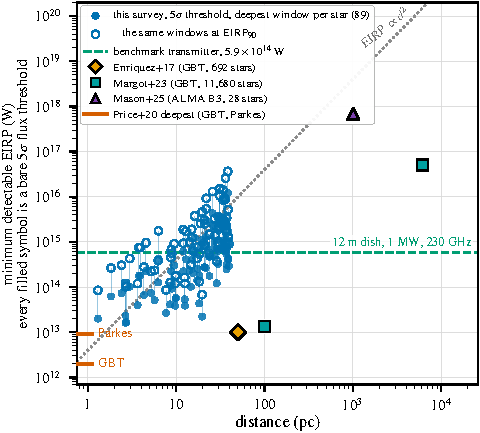
\includegraphics[width=\columnwidth]{figures/eirp_context_a.pdf}\\
{\footnotesize (a)}\\[4pt]
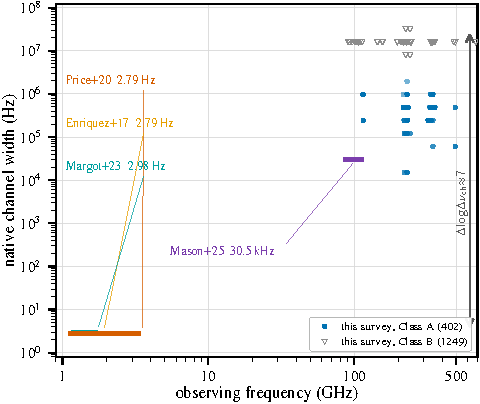
\includegraphics[width=\columnwidth]{figures/eirp_context_b.pdf}\\
{\footnotesize (b)}
\caption{Where this survey sits among published radio technosignature
searches. \textbf{(a)} Minimum detectable EIRP against distance. Blue,
this survey, the deepest window per star: \emph{filled}, that window's bare
$5\sigma$ threshold, which is the quantity the other programmes quote;
\emph{open}, the same window at $\mathrm{EIRP}_{90}$, joined to its own
filled symbol. Orange, \citet{Enriquez2017}; aqua, \citet{Margot2023};
violet, \citet{Mason2025}; left-edge ticks, \citet{Price2020}, all at their
own $5\sigma$ thresholds. Grey dotted, EIRP $\propto d^{2}$ at constant
received flux; green dashed, the illustrative \BenchDiam\,m
benchmark transmitter of \S\ref{sec:excludes}. The ordinates are
commensurable as total powers for a sub-channel carrier, and the filled
symbols make the comparison on one convention; the gap to the open symbol
is what completeness costs.
\textbf{(b)} Native channel width against observing frequency for every
searched window (filled, Class~A; open, Class~B), with the
comparison programmes as horizontal segments. This survey's own widths span
\SzChanDexSurvey{} orders of magnitude; the
$\Delta\log\Delta\nu_{\rm ch}\approx7$ annotation marks the span that
opens once the comparison programmes' channels are set beside them: the
channelisation, not the plotted power, is what differs most between
programmes.}
\label{fig:context}
\end{figure}

A non-detection becomes a quantitative statement only through a stated
search volume. \citet{Wright2018} formalised that volume, and
\citet{Margot2023} its conversion into an upper bound on the fraction of
stars hosting a transmitter; \citet{EarthDetectingEarth2025} asked where
Earth's own technosignatures would be detectable. Such a bound is valid
only if the sample represents the population it is meant to describe.
This sample was assembled by other observers for other purposes, so it
does not, and \S\ref{sec:sample} states what it is instead.

%% Housekeeping, v4.12: the three standing REQUESTs that lived here are now
%% moot. app_D, app_E and app_F have been deleted, so fig:contextapp and the
%% three unlettered \ref{fig:context} citations they carried are gone with
%% them; 05_results.tex writes Fig.~\ref{fig:context}(a) in full.
%% STILL OPEN, and queued for the sensitivity owner rather than repeated
%% here: referee 2's figure point 1 asks that panel (a) plot this survey's
%% 5 sigma EIRP_trig as the filled symbol, for a like-for-like comparison
%% with the other programmes' bare thresholds, and EIRP_90 as a second open
%% symbol on the same points. The caption above already concedes that the
%% conventions differ, which is the concession the referee is declining to
%% accept; it must become two symbols, not a sentence.
%% The Mason matched-received-flux comparison is made here and nowhere else;
%% \S6 cites this section for it. The benchmark is evaluated once, in
%% \S\ref{sec:excludes}, and is labelled illustrative in both places it is
%% named.
%
\section{The sample}
\label{sec:sample}

This search covers \NWindows{} spectral windows toward \NStars{}
stars in \NSystems{} systems within 40\,pc, drawn from \NEB{}
public ALMA execution blocks and \TotalDataTB\,TB of raw data through one
frozen pipeline, \StTelHours\,h of telescope time and \LdgCensusHours\,h
summed over windows. We call that set the
\emph{primary census}, and it is the set every limit, every crossing and
every expectation in this paper is computed over. Four further sets of blocks
enter the paper --- a hold-out reserved before any block on its own side of the rule was
searched, an
archival extension searched afterwards, an out-of-sample control beyond
40\,pc, and an external sample used only to calibrate the spatial statistic
--- and none of them is part of the primary census.
The primary census is \LdgCensusEB{} execution blocks, \LdgCensusWin{}
searched windows, \LdgCensusStars{} stars in \LdgCensusSys{} systems and
\LdgCensusHours\,window-hours; the hold-out is \LdgHoldEB{} blocks and
\LdgHoldWin{} windows, and the archival extension \LdgExtEB{} blocks and
\LdgExtWin{} windows.
Table~\ref{tab:blockledger} gives all five sets in rows that sum, with the
results each one enters; wherever a number in this paper is computed over
something other than the primary census, that table's name for it is used at
the point of use.

Three words are used consistently and are not interchangeable. A \emph{star}
is an individual stellar component; a \emph{system} is a gravitationally
bound group, counted once however many of its components were observed; a
\emph{target} is one ALMA pointing. The census holds \NStars{} stars
in \NSystems{} systems.

The census is two experiments, not one. \NWinA{} windows toward
\LdgClassAStars{} stars in \NSysClassA{} systems are fine-channel, called
\emph{Class~A} throughout: these resolve a drifting carrier and are the
primary experiment, and every sensitivity and every exclusion quoted here
refers to them unless stated otherwise. The remaining \NWinB{} windows
are coarse-channel, \emph{Class~B}, and support a secondary search for
unresolved spectral excess; they can register a spike but cannot distinguish
a drifting signal from a stationary one.

The inclusion criteria are objective and were applied by query. A star enters
if its Gaia~DR3 parallax is at least 25\,mas, measured to better than
\PlxAdqlPct{} per cent, and if its proper-motion-corrected position at the
observation epoch falls inside the quoted field of view of at least one
public execution block. Distances are direct inversions, $d=1/\varpi$, and
the star need not sit at the pointing centre. Disc, planet and spectral type
enter as descriptive metadata only, and no star or window was excluded by an
unlisted criterion or for short integration. The parallax criterion never
binds: the worst fractional parallax error among the stars searched is
\SfPlxWorstPct{} per cent, an order of magnitude inside it, and inside the
stricter $\sigma_\varpi/\varpi\le\SfPlxCutDec$ used in
Table~\ref{tab:selfunc} to select a reference census on the same footing.
The query returns
\NCensus{} work-list entries; the quoted field of view is optimistic, and
only \NGenuinelyCovered{} of those stars are in fact contained by a public
field, of which \NStars{} yielded a searchable window. The per-star and
per-window ledger, including the five-criterion decision tree and every edge
case, is in the data release.

\subsection{The archival selection}
\label{sec:bias}

This sample was not designed. It is whatever previous ALMA programmes
happened to observe, for their own reasons, and \PctDiscProposal{} per cent
of the stars searched were targeted under a debris-disc or planet-formation
proposal. The resulting bias is strong and measurable, and
Table~\ref{tab:selfunc} tabulates it against a volume-limited reference
census selected on the same parallax quality.

\emph{The dominant selection effect is distance.} Stars within 5\,pc are
over-represented by a factor \SfTopRatio, and the enhancement falls
monotonically with distance to a factor of two \emph{under}-representation
beyond 30\,pc. Spectral type comes second: A~stars are over-represented by
about \SfARatio{} and F and G stars by factors of two to three, because those
are the stars with bright debris discs. M~dwarfs are mildly depleted ---
\SfMSearched{} of the \SfNStar{} searched stars are M~dwarfs, a factor
\SfMRatio{} of their share of the reference census, and only
\SfMClassAStars{} of them carry the fine-channel coverage that can resolve a
drifting carrier at all --- and that is a weaker
statement than the table's early-type ratios, not a stronger one. Both
figures are bounds in the same direction: Gaia temperatures are missing for
about half the reference census and missing preferentially for the coolest
objects, so the census M~fraction is a lower limit and every early-type ratio
is therefore a lower limit too. Coverage is also concentrated:
\ConcThreeWin{} of the \NWindows{} windows come from \ConcThreeSys{}
systems. Every statistical statement in this paper is therefore a statement
about an archive-selected sample of nearby stars, and none of them is an
occurrence rate for the solar neighbourhood. The systems a targeted search
would itself have chosen --- every sample system within 15\,pc with a confirmed
planet --- are listed in the data release, where \CsIntNoClassA{} of the
\CsIntNRow{} carry no Class~A coverage at all and so no drift-resolving limit:
the archival selection acting on exactly the targets a transmitter search
would pick.

%% GENERATED by selfunc_v411.py -- do not hand-edit.
\begin{table}
\centering
\scriptsize
\setlength{\tabcolsep}{4pt}
\caption{Selection function of the searched sample against a volume-limited reference census, both selected on the same parallax quality: Gaia~DR3 sources with $\varpi>0$, $\sigma_\varpi/\varpi\le0.1$ and $1/\varpi\le40$\,pc (17\,566 objects, 8594 of them carrying a \texttt{teff\_gspphot} estimate), against the 89 stars with at least one searched window. The searched stars are measured far better than the cut requires --- the worst fractional parallax error among them is 2.5 per cent --- so the two columns are selected alike, and loosening the cut to 0.2 adds no census object at all. 86 of the 89 searched stars are classified: 53 from the Gaia temperature, 25 from the SIMBAD spectral type where that temperature is absent, and 8 identified as white dwarfs; 3 carry no classification in either source. The SIMBAD route matters because \texttt{teff\_gspphot} is missing preferentially for cool stars, which is the population the M~dwarf statement is about. ``Ratio'' is the sample column fraction over the census column fraction; $>1$ is over-representation. \emph{The strongest selection effect here is distance, not spectral type.}}
\label{tab:selfunc}
\begin{tabular}{@{}lrrr@{}}
\toprule
Property & Census & Searched & Ratio \\
\midrule
\multicolumn{4}{@{}l}{Distance} \\
\quad $d\le5$\,pc & 48 (0.3\%) & 12 (13.5\%) & 49.3 \\
\quad 5--10\,pc & 240 (1.4\%) & 13 (14.6\%) & 10.7 \\
\quad 10--20\,pc & 2069 (11.8\%) & 18 (20.2\%) & 1.7 \\
\quad 20--30\,pc & 5391 (30.7\%) & 19 (21.3\%) & 0.7 \\
\quad 30--40\,pc & 9818 (55.9\%) & 27 (30.3\%) & 0.5 \\
\midrule
\multicolumn{4}{@{}l}{$T_{\rm eff}$ class$^{a}$} \\
\quad A & 24 (0.3\%) & 5 (6.4\%) & 23.0 \\
\quad F & 402 (4.7\%) & 9 (11.5\%) & 2.5 \\
\quad G & 860 (10.0\%) & 16 (20.5\%) & 2.0 \\
\quad K & 1400 (16.3\%) & 7 (9.0\%) & 0.6 \\
\quad M & 5908 (68.7\%) & 41 (52.6\%) & 0.8 \\
\midrule
\multicolumn{4}{@{}l}{Other axes} \\
\quad Confirmed planet hosts$^{b}$ & 26 (15.5\%) & 23 (25.8\%) & 1.7 \\
\quad White dwarfs$^{a}$ & -- & 8 (9.0\%) & -- \\
\quad Searched stars / systems & -- & 89 / 82 & -- \\
\bottomrule
\end{tabular}

\smallskip
{\footnotesize $^{a}$Temperature bins, not MK types: A $\ge7500$, F 6000--7500, G 5300--6000, K 3900--5300, M $<3900$\,K, normalised over the 78 classified non-degenerate stars. The 8 white dwarfs are kept apart because a degenerate is not an early-type star and its photometric temperature would place it among them. Gaia \texttt{teff\_gspphot} is unavailable for about half the reference census, preferentially for the coolest and faintest objects, so the census M fraction is a lower limit and every earlier-type ratio in this panel is correspondingly a lower limit; the searched column has no such gap.\\ $^{b}$Both columns are the same positional join, of the 168-entry ALMA-covered work list and of its searched subset, to the NASA Exoplanet Archive \texttt{pscomppars} table accessed 2026 October 4; a confirmed planet is a row of that table. The 23 searched hosts carry 50 confirmed planets between them, and 21 of the 23 survive the deuterium-burning mass limit. The Gaia reference census carries no planet information, so the census column in this row is the work list rather than the 17\,566-object Gaia census.}
\end{table}


%% fig:funnel DELETED: it drew the three counts the sentence above it
%% already carries, so it joined the prose instead of replacing it.  The
%% artwork is online material (figures_diagnostic/selection_funnel.pdf).

\subsection{Frequency coverage and archival scope}
\label{sec:coverage}

The Class~A experiment covers $\Delta\nu_A=\DnuA$\,GHz of unique sky
frequency, and that coverage is sparse: it is \DomAIslands{} disjoint islands
scattered between \DomAFreqLo{} and \DomAFreqHi\,GHz, not a band. The
endpoints are a range over which observations exist, never a range that was
covered. Adding the coarse-channel windows brings the total archival coverage
to \DnuAB\,GHz in \UnionIntervals{} intervals, of which \SearchedUnionGHz\,GHz
survives the molecular-line mask of \S\ref{sec:method}. The distribution is
shown in Fig.~\ref{fig:waterfall}; a transmitter at a frequency between the
islands was never observable here, whatever its power.

The archive is not exhausted either, and the shortfall is accounted for
rather than estimated. \LdgExtScope{} further blocks lie inside the same
query but were not processed when the census was frozen;
Table~\ref{tab:blockledger} gives what became of each. \LdgExtSearched{} of
them have since been calibrated and searched, and they enter this paper only
as repeat epochs. The largest single gap is the \FateNoCal{} blocks for which
the archive holds raw visibilities that were never pipeline-calibrated,
\FateNoCalGB\,GB in all; no effort on our side would close it.

\begin{figure*}
\centering
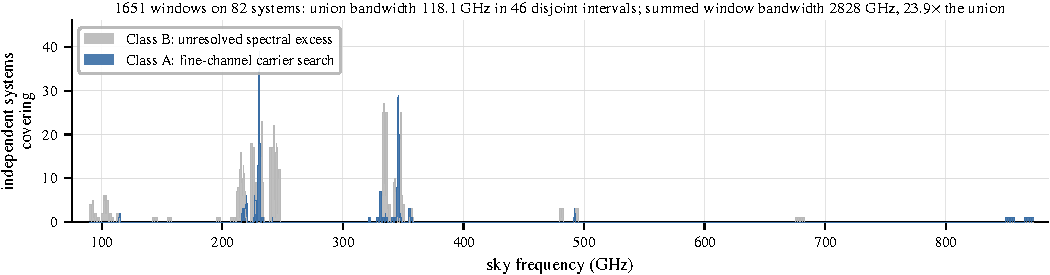
\includegraphics[width=0.99\textwidth]{figures/coverage_waterfall.pdf}
\caption{Where this survey searched. \emph{Lower panel:} each searched
window is a horizontal segment on its host system's row, rows ordered by
distance and labelled alternately on the left and right axes; heavy blue
marks the fine-channel carrier search (Class~A) and light grey the
coarse-channel spectral-excess search (Class~B). \emph{Upper panel:} the number
of systems covering each gigahertz of sky frequency; the threshold
distribution is Fig.~\ref{fig:context}(a). The coverage is narrow, clustered
and repeatedly revisited: \UnionIntervals{} islands concentrated near 230
and 345\,GHz, with summed window bandwidth $\GrossOverUnion\times$ the
union. The union measures frequency coverage, the summed bandwidth
integrated search effort.}
\label{fig:waterfall}
\end{figure*}

%% tab:blockledger MOVED to Appendix A (sections/app_A_reproducibility.tex).
%% The headline rows are carried in the prose of Sec. 3.1 so that the
%% cross-reference is not a pointer with no numbers beside it, which is
%% what R2-M2(a) asked for when it asked for the ledger early in Sec. 3.

%% tab:interesting MOVED TO THE DEPOSIT: an explicitly illustrative table
%% ("systems a targeted search would itself have chosen"), already
%% deposited row for row.  tab_interesting.tex is still generated.

%% v4.11 LENGTH (Ruling 4): tab:searchspace is DELETED.  Nothing cited it --
%% `labelcheck` F4 and `xrefcheck` both reported it as typeset and never
%% referenced, which is what an owner's last citation being removed looks
%% like.  Its counts of blocks, windows, stars and systems are
%% Table~\ref{tab:blockledger}'s, its frequency unions are stated in the
%% text above and drawn in Fig.~\ref{fig:waterfall}, and its channel
%% widths and drift range are in \S\ref{sec:method}.

%% REQUEST (numbers owner): tab_interesting.tex is generated by
%% referee_r9/sample/mk_interesting.py, which reads the released
%% catalogue, the frozen census, the confirmed-planet table and
%% \SelRatioRank out of the macro layer. Please adopt it into make_all.sh so
%% the table regenerates with everything else, and point its planet column at
%% r10inputs/nea_pscomppars_60pc_v411.csv (the dated NASA Exoplanet Archive
%% extract selfunc_v411.py uses) rather than at the older unique-host file,
%% so one definition of "confirmed planet" serves both tables. Two display
%% defects in it are yours, not mine: the catalogue designation of Barnard's
%% Star prints as a SIMBAD identifier with the "NAME" prefix stripped, and
%% BD+05 1668 would read better with its GJ alias beside it. Both belong in
%% star_alias.designation.
%
\section{Data and methodology}
\label{sec:method}

The search looks for one kind of signal: an unresolved carrier at the
star's own position, narrow compared with a single correlator channel, and
drifting in sky frequency because the transmitter accelerates along the line
of sight. Over a long track its power is spread across many channels, so a
search that treats each channel on its own will miss it. The analysis
de-drifts the data before it measures them.

\subsection{The de-drifted search statistic}
\label{sec:statistic}

Each window's dynamic spectrum is stacked along every trial drift rate
$\dot\nu$. The search statistic is the largest stacked signal-to-noise
ratio anywhere on the resulting channel$\times$drift grid,
%
\begin{equation}
T(\mathbf{x})=\max_{\dot\nu,\;\nu}\;
\frac{\sum_{t} I\!\left(\mathbf{x},t,\nu+\dot\nu t\right)\big/\sigma^{2}(t,\nu)}
     {\left[\sum_{t}1\big/\sigma^{2}(t,\nu)\right]^{1/2}},
\label{eq:tstar}
\end{equation}
%
where $I(\mathbf{x},t,\nu)$ is the spectrum at sky position $\mathbf{x}$
in integration $t$ and channel $\nu$, and $\sigma(t,\nu)$ is the noise scale
there. Equation~\ref{eq:tstar} is the matched filter for a constant-drift
carrier: it adds the signal coherently along the track and divides by the
noise of the stacked spectrum, so $T$ is an absolute signal-to-noise ratio
and not a local contrast. The noise scale is the median absolute deviation
across \NCtrl{} control positions at each integration and each channel,
scaled to its Gaussian-equivalent standard deviation --- local in time and
frequency, global in position, shared by the star and every control, and with
the across-position median never subtracted from the numerator. The statistic
is evaluated at one position at a time, identically at the star and at each
control, which is what makes the two comparable. $T_\star$ denotes its value
at the star.

Spectra are extracted at the star's apparent position, never from images.
For each integration and each native channel the pipeline forms the weighted
vector average of the phase-shifted visibilities, in total intensity: the
mean $I=(XX+YY)/2$ of the two parallel-hand correlations. That average is the
dirty-map value at the extraction position --- an amplitude, not a
deconvolved flux density, so in a field with extended emission it is not a
point-source measurement. The data are used as the archive delivered them,
through ALMA's own calibration and quality assurance, with their flagging
carried through, every delivered channel searched, and no regridding,
deconvolution or edge trimming. A per-integration median along the
\emph{frequency} axis removes the continuum; no median is taken along
time, so a one- or two-channel feature cannot be removed by it. One
subtlety matters for every power quoted below: the delivered channels are
smoothed, so a channel's effective noise bandwidth is not its separation and
flux density times channel width is not yet a radiated power. A response
correction computed from the correlator's own channel shape supplies the
difference, derived and validated against the effective resolutions ALMA
reports in Appendix~\ref{app:conventions}.

One convention is fixed here and holds everywhere in the paper. The search
runs on the topocentric sky frequencies ALMA delivered, and every drift rate
quoted is the apparent one at the telescope, since that is what the data
contain and what a reader can recompute from the released channel axes. Two
steps need the star's own frame instead, and both take it: a crossing is
compared with the line catalogue, and a repeat epoch is read at the predicted
cell, after each block's frequency axis has been corrected for the Earth's
motion at that epoch and then for the star's systemic velocity. Nothing here
is evaluated in a barycentric frame alone.

Two power quantities carry the main text, both defined in
Table~\ref{tab:quantities}: the trigger level $P_{\rm trig} = 4\pi
d^{2}S\,\Delta\nu$ at distance $d$, for a carrier that makes $T_\star$ reach
$T_{\rm trig}=\StageNullTrig$ in one native channel of width $\Delta\nu$,
and the sensitivity $\mathrm{EIRP}_{90}$. The second is measured, not
assumed: synthetic carriers of known amplitude were injected into
calibrated visibilities and recovered through the unmodified pipeline,
\SelNTone{} of them over \SelNUnit{} block--window configurations of the
fine class and \SensNToneCoarse{} over \SensNInjCoarse{} of the coarse,
spanning both ALMA arrays, four bands and the sample's full range of
channel widths. Every limit quoted in
this paper is the $\mathrm{EIRP}_{90}$ of its own window, given to two
significant figures beside its native channel width; the measured
completeness is \S\ref{sec:pninetysel} and its error
budget is Table~\ref{tab:p90budget}. The absolute flux scale is checked twice from
outside, in two bands on two arrays: the extractor reproduces an
independent reduction of the same AU~Mic visibilities to
\PxJanRatio\,$\pm$\,\PxJanRatioErr, and the published quiescent flux
density of $\epsilon$~Eridani to \PxEpsRatio\,$\pm$\,\PxEpsRatioErr{}
\citep{Burton2022}.

The drift range searched is bounded by an acceleration, not by a
frequency. Drift rate and line-of-sight acceleration are one quantity in
two sets of units, $a_{\rm los}=c\,\dot\nu/\nu$, so a ceiling expressed
as $\dot\nu/\nu$ is the same physical limit in every band; the released
drift and acceleration ceilings satisfy that relation window by window, to
$\DriftRelDev$ over all \DriftRelNWin{} Class~A windows. The default
ceiling is \DriftCeilLo--\DriftCeilHi\,Hz\,s$^{-1}$\,GHz$^{-1}$, that is
$|a_{\rm los}|\le\AccelCeilMed$--$\AccelCeilMax$\,m\,s$^{-2}$. That is
the acceleration of a transmitter orbiting a solar-type star at a few
hundredths of an au. It is the \citet{Mason2025} fiducial with a
threefold margin, widened for a confirmed exoplanet host whenever the
innermost known planet demands more. It is far narrower than the general
recommendation of \citet{Sheikh2019}, which is set by solar-system
rotation and orbital motion rather than by a planet's own acceleration,
and the difference is a deliberate restriction of what this search covers
and not a weaker version of their advice. The margin is not cosmetic: at unit
margin the search would have been blind to two of the windows that
produced a crossing. The grid is uniform in $\dot\nu$, and fine enough
that a carrier midway between two trials loses no more than
\DriftGridFineHalf{} of a native channel over the longest track. Two limits
follow: the rates searched are the apparent ones at the telescope, so a
deliberately chirped carrier is not distinguished from an accelerating
platform, and a transmitter need not be bound to a known planet at all, so
drifts faster than the ceiling are simply unconstrained
(Fig.~\ref{fig:accel}).

\begin{figure}
\centering
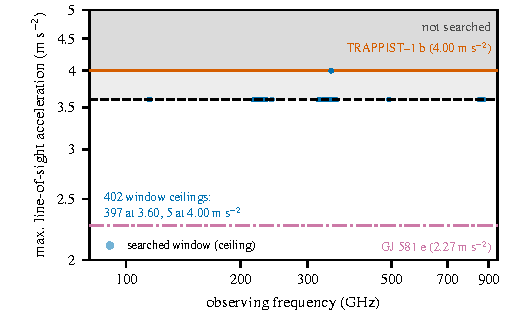
\includegraphics[width=\columnwidth]{figures/drift_acceleration.pdf}
\caption{What the drift search reaches, as a physical selection function.
The drift ceiling of each of the \NWinA{} Class~A windows (points),
converted to line-of-sight acceleration, $|a|=c\,\dot\nu/\nu$, against
observing frequency; the shaded region above is unsearched. The boundary
is flat because the grid was built at constant acceleration; in the units
the search works in it is not, running \AccelDriftLo\,kHz\,s$^{-1}$ at
\AccelFreqLo\,GHz to \AccelDriftHi\,kHz\,s$^{-1}$ at \AccelFreqHi\,GHz.
Horizontal lines are reference accelerations: Earth's rotation at the equator
(\AccelEarthRot\,m\,s$^{-2}$) and orbit (\AccelEarthOrb\,m\,s$^{-2}$), and
the two most demanding known planets of any target, \AccelWorstName{}
(\AccelWorstVal\,m\,s$^{-2}$) and \AccelSecondName{}
(\AccelSecondVal\,m\,s$^{-2}$). The boundary drawn is the default ceiling,
\AccelCeilMed\,m\,s$^{-2}$, which is also the median; it runs to
\AccelCeilMax\,m\,s$^{-2}$ on the \AccelNWide{} \AccelWideStar{} windows. For
the most demanding case, transiting TRAPPIST-1~b, \TrapPhaseHi{} per cent of
the orbital phase lies above the default ceiling and \TrapPhaseLo{} per cent
above the widened one.}
\label{fig:accel}
\end{figure}

Only part of the archive can carry a drift search at all, and the two
classes reported here are that division (Table~\ref{tab:quantities}).
Channelisation in the sample is bimodal, with an empty gap between the modes,
so the split is unambiguous, and it coincides with the physical criterion
that matters: whether the maximum searched drift crosses of order one channel
or more over the on-source track, $\eta_{\rm drift} =
|\dot\nu_{\max}|\tau_{\rm track}/\Delta\nu_{\rm ch} \gtrsim 1$. Each
window's own $\eta_{\rm drift}$, trial-drift count and acceleration ceiling
are released catalogue columns, so a reader may reclassify on that criterion
instead; the two do not partition the survey identically. \textbf{The two
classes are physically different experiments}, results are given per class,
and they are combined only where that is statistically appropriate.

\subsection{From a crossing to a confirmed signal}
\label{sec:summary}

Every window passes through the same three tests in the same order, and
three words name what comes out of them: a \emph{crossing}, an
\emph{unattributed crossing} and, had one survived, a \emph{confirmed
signal} (Fig.~\ref{fig:chain}). Each is set out below as the quantity it
measures, the number that quantity is compared with, when that number was
fixed, and what passing it does and does not establish. There is no fourth
test, and none of the three is a significance test.

\begin{enumerate}[label=(\roman*),leftmargin=1.9em,itemsep=3pt,topsep=3pt,parsep=0pt]
\item \emph{Trigger $\to$ a crossing.} The quantity is $T_\star$, the
de-drifted statistic of Eq.~\ref{eq:tstar} read at the stellar position; the
criterion is $T_\star\geq T_{\rm trig}=\StageNullTrig$ in at least one
channel$\times$drift cell; and both the statistic and the level were fixed
before the archival search began. \textbf{$T_{\rm trig}$ is a trigger
threshold and not a detection significance:} $T$ is not shown to follow any
standard distribution under the null, so the level carries no tail
probability, and a window holds between \TuCellsLo{} and $\TuCellsHi$ of
those cells, so one level buys very different protection in a coarse
single-pointing window and in a finely channelised one on a long track. A
crossing establishes only that the window goes on to the next two tests.
\item \emph{Line attribution $\to$ an unattributed crossing.} The quantity
is the crossing's velocity offset from the nearest transition of a
molecular-line catalogue, evaluated in the star's own rest frame; the
criterion is $\pm\MaskHalfKms$\,km\,s$^{-1}$. The statistic, the trigger and
the original species list were fixed before any crossing was classified; the
species list was afterwards extended, and that extension is the reason one
crossing is reported as unattributed where the list as it now stands would
attribute it (Appendix~\ref{app:linemask}). The half-width follows the Keplerian line-of-sight velocities of gas
surviving beyond a few au, with margin for the systemic velocity. A crossing
inside that window is \emph{attributed}, and the attribution is good
evidence: a coincidence with a catalogued transition makes an astrophysical
origin far more plausible than a transmitter, the more so where a second
transition of the same species or known circumstellar emission is present.
But a coincidence is a statement about a catalogue rather than a property of
a frequency, so this is an attribution and not an exclusion, and
\textbf{every crossing goes on to the recurrence test whichever side of the
window it falls}, wherever a later block covers the frequency. An unattributed crossing is a target for follow-up and not
a detection. The window's price is that the survey constrains nothing inside
it: ${\approx}\SearchedUnionGHz$\,GHz of the \UnionGHz\,GHz covered lies
outside (Appendix~\ref{app:linemask}).
\item \emph{Independent recurrence $\to$ a confirmed signal.} The quantity is
$T_\star$ at the cell the first epoch predicts, read in another execution
block of the same star at a single drift rate after the frame correction of
\S\ref{sec:statistic}; the criterion is that it reach the trigger again; and
the test was specified before the repeat epochs were searched. It is a weak
criterion, and the archive's uneven temporal sampling is why: only part of
the sample has epochs separated well enough to apply it at all.
\end{enumerate}

\emph{Two diagnostics hang off the second test, and the word is exact: each
says which crossing deserves attention first, and neither decides anything.}
The first ranks $T_\star$ against the same statistic at \NCtrl{} control
positions in the same window, drawn once from a fixed seed into an annulus
placed by each block's own synthesised and primary beams so that no control
sits on the star; its lowest value, $1/(\NCtrl+1)$, means the star beat every
control. It is a ranking filter and not a significance test, because the
stellar and control positions are not demonstrably exchangeable: out of
sample, on \HoWin{} windows the frozen pipeline had never seen, the stellar
rank has median \HoRankMed{} where one half is expected if the two were
interchangeable, and a parameter-free correction for the annulus geometry
does not restore an exchangeable statistic (Appendix~\ref{app:radius}). It
also responds to compactness rather than to origin, as $\beta$~Pictoris
shows: genuine carbon monoxide ranks below its own control ring there,
because the resolved disc lifts the ring along with the star. The second
diagnostic is a visibility-domain fit, which asks whether a crossing's
emission is at the stellar coordinates rather than elsewhere in the field; it
cannot discriminate at the trigger either, because a noise maximum at the
star has flux at the star (\S\ref{sec:vistest}). \textbf{Neither gates a
disposition, so neither is charged to the sensitivity}, and the limits here
are correspondingly deeper than a chain charging for the rank would give.
Throughout, $p$ denotes a genuine significance level, and no probability
computed against the rank's own null is called one.

\emph{One execution block is not a null, and a rule fixed in advance says so.}
The comparison with the control positions needs each block's ensemble to behave
like noise, and a block fails when the median control statistic over its own
windows, scaled by the median of that quantity over its class, exceeds
\BqFactor{} that scale. Of the \BqNBlocks{} primary-census blocks, \BqNFail{}
fails --- \BqFailBlock{} toward \BqFailStar, at \BqFailQ{} where the next worst
is \BqNextQ. \textbf{The Class~A results are identical with it and without it},
the same \BqWinACut{} windows and \BqXrossACut{} crossings either way, because
its \BqFailNWin{} windows are all coarse-channel; what it does hold is
\BqFailNCross{} of the \NCross{} crossings, the survey's entire Class~B
crossing population (Appendix~\ref{app:falsealarm}).

Because a fixed threshold is not a fixed false-alarm rate, the number of
crossings expected by chance is computed window by window, from the
exceedance rate measured at each window's own control positions; the reserved
blocks then test the one assumption that makes, which is that a star behaves
like a control position in its own field (\S\ref{sec:trigunif}).

Three corrections precede the statistic: the extraction field is chosen so
that the star lies inside the delivered primary-beam field and not merely
inside the quoted field of view; the stellar position is propagated to the
observation epoch for proper motion, though not for the annual parallax,
whose omission is corrected window by window in
\S\ref{sec:pninetysel}; and on-source time is accounted per integration
from the
delivered exposure records rather than from the scan intentions. That the
chain finds what it is meant to find is shown twice over, by the injected
carriers above and by $\beta$~Pictoris CO --- a real feature at a known
stellar position, recovered and localised in two transitions and
\NStageOneBpicEb{} execution blocks (\S\ref{sec:bpicval}).

\begin{table}
\centering
\caption{The quantities and the three words this paper uses, defined once.
Every term below is used in this sense throughout and in no other.}
\label{tab:quantities}
\small
\begin{tabular}{@{}p{0.235\columnwidth}p{0.70\columnwidth}@{}}
\hline
Term & Definition \\
\hline
Crossing &
A channel\,$\times$\,drift cell at the stellar position reaching
$T_\star\geq\StageNullTrig$. An event requiring investigation; no claimed
significance. \\
Unattributed crossing &
A crossing lying more than $\MaskHalfKms$\,km\,s$^{-1}$ in the star's frame
from every transition of the frozen line catalogue. A target for follow-up;
not a detection. \\
Confirmed signal &
An unattributed crossing recovered at the predicted stellar-frame frequency
and drift in an independent block. The only confirmation criterion. \\
$P_{\rm trig}$ &
The power of a carrier that makes $T_\star$ reach the trigger in one native
channel. An internal pipeline level: not a sensitivity, not a
significance. \\
$\mathrm{EIRP}_{90}$ &
The power at which nine injected carriers in ten are recovered at the star
through the trigger. A measured completeness, not a detection probability. \\
Class~A &
The primary experiment: \NWinA{} fine-channel windows, median
\ChanAMedKHz\,kHz, toward \NSysA{} systems over \UnionClassA\,GHz of union
bandwidth, in which the searched drift crosses of order a channel or more. \\
Class~B &
The secondary experiment: \NWinB{} coarse-channel windows, mode
\ChanBModeMHz\,MHz, constraining a persistent unresolved excess. No drift
discrimination, and never a carrier search. \\
The sample &
Neither volume-limited nor representative of the solar neighbourhood: the
stars ALMA happened to observe for other reasons (\S\ref{sec:sample}). \\
\hline
\end{tabular}
\end{table}

%% HANDOVER (04_method.tex, round 11, r11-chain) -- supersedes the round-10 note.
%% THE CHAIN IS NOW THREE STEPS: trigger -> line attribution -> recurrence.
%%   The rank and the visibility fit are diagnostics attached to the SECOND
%%   step and gate nothing, so nothing in this paper may charge their cost to
%%   a sensitivity, and the word "candidate" is no longer a defined term
%%   anywhere: the three words are crossing / unattributed crossing /
%%   confirmed signal.
%% tab:quantities IS NOW IN THIS FILE and is the single definition of all
%%   eight terms (R1-10).  It is what licenses the deletion of the repeated
%%   caveats elsewhere; the list of repetitions it pays for is entry 7 of
%%   /workspace/SETI/referee_r11/INTEGRATION_QUEUE.md.
%% DELETED to pay for it: the whole of old stage (iii) (the spatial screen as
%%   a gate, 37 lines), the two-stratum EIRP90 sentences, the screen-cost
%%   arithmetic, and the free-standing visibility-check and rank-displacement
%%   paragraphs, both folded into the diagnostics paragraph.
%% STILL OPEN, queued in /workspace/SETI/referee_r11/INTEGRATION_QUEUE.md:
%%  * fig:chain prints as Figure 8 but is first cited here; the float lives in
%%    05_results.tex.  Either file may host it, but it must be renumbered or
%%    moved.
%%  * the third correction below still says the stellar position is
%%    "propagated to the observation epoch".  It becomes "proper motion and
%%    annual parallax both" the moment r11-sens's re-extraction lands (M5),
%%    and not before -- we must not assert a correction we have not applied.
%%  * no Class A EIRP90 multiplier is quoted here ANY MORE, deliberately: one
%%    adopted figure belongs in S5.1 and Table 4 and nowhere else.
%% NUMBERS STILL WANTED here: a macro for the Keplerian half-width (the typed
%%   13 km/s is gone from stage (ii), and so is the figure) and one for the
%%   threefold drift margin.
%% Table 10 (tab:algorithm) in App A remains unreferenced -- its citations
%%   were here and the three-step chain replaces it; the appendix owner should
%%   delete the float.
%
\section{Results}
\label{sec:results}

The primary experiment is the Class~A search for a drifting, unresolved
spectral carrier: \NWinA{} fine-channel windows toward \NSysClassA{}
systems. The Class~B search for an unresolved spectral excess is secondary
and carries no drift discrimination: \NWinB{} coarse windows. Together they
are the \NWindows{} windows of the released catalogue. \textbf{No event
satisfied the confirmation criterion set out in \S\ref{sec:summary}.} What
follows is first how deep the search reaches, and then what it found and how
each finding was disposed of.

\subsection{Sensitivity: the power at which a carrier would have been
found} \label{sec:pninetysel}

\emph{The sensitivity of this survey is a measured completeness and not a
threshold.} Artificial carriers were added to the real calibrated
visibilities at a random sub-channel phase and a random drift from each
window's own grid and recovered through the unchanged pipeline; the power at
which nine in ten come back is $\mathrm{EIRP}_{90}$, the only sensitivity
quoted here. \emph{It is measured through the chain the survey applies} ---
the trigger and localisation at the stellar position. The \NCtrl-position
spatial rank annotates a crossing rather than deciding it
(\S\ref{sec:summary}) and is not charged against it: it would cost a further
factor $\SensCostLike$ and in \SensNRingHiUnres{} bright-ring windows could
not be met at any injected power (Fig.~\ref{fig:strata}), and a limit should
not be charged for a gate that disposes of nothing.

\emph{Measured that way the completeness is one number.} Nine carriers in ten
are recovered at $\SensMultA\,P_{\rm trig}$, where $P_{\rm trig}$ is the
window's own trigger power, and that class-average factor is determined to
$\pm\SensBootPct$ per cent. Every one of the \SensNInj{} directly injected
Class~A windows resolves a ninety per cent point of its own, between
$\SensIndivLo$ and $\SensIndivHi\,P_{\rm trig}$, and the value does not
depend on the brightness of the window's control ring: the \SensNRingHi{}
windows whose ring carries resolved emission come back at
$\SensRingHi\,P_{\rm trig}$ against $\SensRingLo$ for the rest
(Fig.~\ref{fig:strata}). One factor therefore serves the class. Class~B
carries
its own factor $\EirpNinetyMultB\,P_{\rm trig}$, measured the same way from
\SensNToneCoarse{} carriers injected into \SensNInjCoarse{} coarse windows of
\SensNInjCoarseBlock{} execution blocks and weighted by the coarse
catalogue's own distribution of ring brightness; it is what sets the limits
for Barnard's Star, Wolf~359 and Proxima.

\emph{The resulting limits.} The median Class~A window reaches
$\EirpNinetyWinMedA$\,W of equivalent isotropic radiated power and the median
system, on its best window, $\EirpNinetySysMedA$\,W, with a spread across
systems of $\EirpNinetySysLoA$--$\EirpNinetySysHiA$\,W
(Fig.~\ref{fig:classasens}a). The round $10^{15}$\,W level is reached for
\NSysEfifteen{} of them. Table~\ref{tab:p90budget} collects the terms acting
on those numbers. The calibration of the factor is good to
$\times\SensFacLo$--$\times\SensFacHi$, and that is the interval which
applies to the median and to the counts. One bias is not inside it and runs
one way only: an injected carrier is added to visibilities that have already
been calibrated and so suffers no atmospheric or instrumental decorrelation,
whereas a real carrier does, so \textbf{every limit in this paper is
optimistic by up to \SensDecorPct{} per cent} on that account --- a figure
declared from the literature rather than measured here.

\emph{Carriers were injected directly into \SensNInj{} of the \NWinA{}
Class~A windows, \SensNInjPct{} per cent, and the result transferred to the
remaining \SensNTransfer, which is the dominant caveat on all of the above.}
The injected windows are the Class~A windows of execution blocks drawn in a
stratified random order fixed in advance, without reference to which windows
hold a crossing; they hold \SensNCrossAch{} crossings against the
\SensNCrossExp{} the population rate predicts. \emph{The unit is the block
and not the window}, because a block's calibrated visibilities are what an
injection campaign has to rebuild: band and array were controlled by the
draw, while channel width, ring brightness and integration length vary inside
a block and were only compared with the population afterwards, agreeing to
\SensCovWorstPct{} per cent on the worst axis.

\emph{Every limit therefore rests on the class-average calibration, and what
one window may differ from it by is a separate statement.} The median ninety
per cent point differs by \SensBandSpread{} between bands,
\SensChanSpread{} between channel widths and \SensArrSpread{} between the two
arrays. The largest of the three is the \SensCovAxis, and none of them is as
large as the gate the chain no longer charges for. The array difference
survives setting the bright-ring windows aside --- \SensArrSpreadFaint{}
without them --- so it belongs to the array and not to its fields, as a
compact array keeping more extended emission inside its beam would.
Across the injected windows as
a whole the ninety per cent point ranges from $\times\SensIndivFacLo$ to
$\times\SensIndivFacHi$ of the adopted factor, so an individual uninjected
window's own completeness is not known to the precision of the interval that
applies to the class.

\emph{One geometric term acts window by window, and it is measured rather
than modelled.} The phase centre assumed in the search omits the annual
parallax, which displaces the star by a median \SensBeamsMed{} of a
synthesised beam and at most \SensBeamsMax. Each limit is therefore divided
by the amplitude a compact source retains at its own displacement --- read
off an injection into the same visibilities at both positions, not off a beam
model (Appendix~\ref{app:conventions}) --- which makes the median Class~A
limit shallower by \PxaShiftWinPct{} per cent. One window,
\PxaMissingStar{} in \PxaMissingEb, has no astrometric keys and is left
uncorrected.

\emph{A carrier that is not always radiating is penalised in proportion.} The
de-drifted stack is coherent across a whole execution block, so a carrier
present for a fraction of one contributes to that fraction of the
integrations and comes back at that fraction of its continuous amplitude.
Over \DutyNTrial{} trials in \DutyNWin{} windows of \DutyNStar{} stars, at
\DutyNCycle{} duty cycles within a track down to \DutyCycleMinPct{} per cent
and at amplitudes between $\times\DutyAmpTrigLo$ and $\times\DutyAmpTrigHi$
of each window's own trigger, the recovered amplitude followed the duty cycle
to \DutyAttenDevPct{} per cent. A transmitter radiating a tenth of the time
therefore needs $\DutyPowFac\times$ the power quoted above, and because those
trials carry no drift the joint drifting and intermittent case is not
measured here at all.

\begin{table}
\centering
\scriptsize
\caption{What sets $\mathrm{EIRP}_{90}$, and in which direction. The
uncertainty on the calibration is an uncertainty on the class-average factor,
and so on any statistic formed over many windows; the spread between windows
is an observed dispersion and is the statement about one window's own limit;
the signed terms are biases, stated with their direction rather than folded
into an error bar. The channel response is carried by the injections rather
than applied afterwards, so it must not be applied again
(Appendix~\ref{app:conventions}).}
\label{tab:p90budget}
\tiny
\setlength{\tabcolsep}{2pt}
% GENERATED by sens_r11.py -- do not hand-edit.
\begin{tabular}{@{}l@{~~}r@{~~}>{\raggedright\arraybackslash}p{0.37\columnwidth}@{}}
\hline
 & value & what it does to the limit \\
\hline
Class-average completeness & $\times3.03$ & nine carriers in ten recovered at this multiple of a window's own trigger power, over 49 injected Class~A windows \\
\hline
\multicolumn{3}{@{}l}{\emph{Uncertainty on that calibration} (per cent), combined in quadrature} \\
The factor itself & $\pm2$ & sampling error of the pooled value over the 49 injected windows \\
Flux, distance and visibility scale & $\pm9$ & calibration \\
\emph{Combined} & $-9/+9$ & $\times0.91$--$\times1.09$ on the factor, and so on the median limit and on the system counts \\
\hline
\multicolumn{3}{@{}l}{\emph{Spread between windows}. An observed dispersion, not an error bar.} \\
Window to window & $\times0.80$--$\times1.58$ & the 49 injected windows resolve 2.41--4.80\,$P_{\rm trig}$ individually, so an uninjected window's own completeness is not known to the interval above \\
\hline
\multicolumn{3}{@{}l}{\emph{Signed terms}. A bias is not an error bar and is not added to one.} \\
Channel response & $\times\InjPeakAtNinety$ & carried by the injections, so already inside the completeness above \\
\quad its residual & $+\InjShortPct$ & the injected profile falls short of the exact response: \emph{conservative} \\
Primary-beam model & $+0/+10$ & ALMA's beamwidth in place of the pipeline's Airy-null one: nothing in the median window, 4 windows of one star \\
Decorrelation & $+0/+20$ & an injected carrier suffers none and a real one does, so every limit is optimistic by up to this much; declared from the literature, not measured here \\
\hline
\end{tabular}

\end{table}

\begin{figure}
\centering
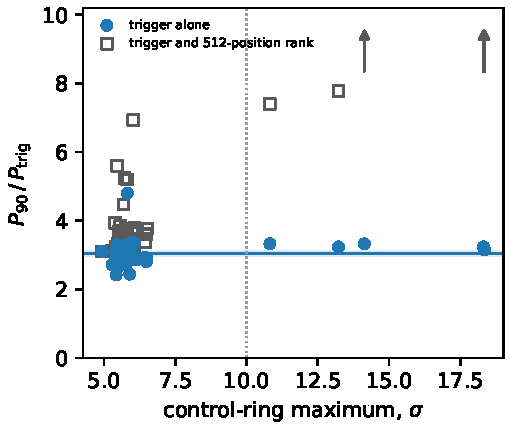
\includegraphics[width=0.96\columnwidth]{figures/sens_ring.pdf}
\caption{Why one completeness factor serves the whole class. Each of the
\SensNInj{} directly injected Class~A windows is plotted at the power that
recovers nine carriers in ten, against the maximum of its own
\NCtrl-position control ring. Filled circles are the criterion adopted
here --- the trigger and localisation at the star --- with the pooled value
and its uncertainty as the line and band; they show no trend with the ring.
Open squares add the demand that the carrier outrank every control position,
and arrows mark the windows that then reach ninety per cent at no injected
power. Dotted, the $\SensRingRule\sigma$ ring brightness above which a ring
carries resolved emission rather than noise.}
\label{fig:strata}
\end{figure}

\begin{figure*}
\centering
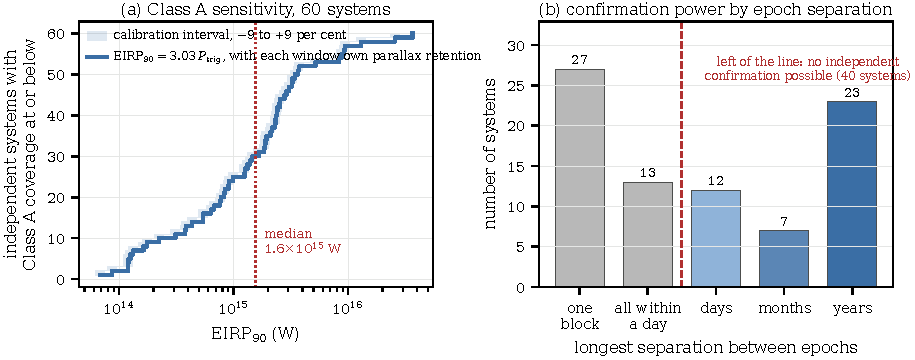
\includegraphics[width=0.92\textwidth]{figures/classa_sensitivity.pdf}
\caption{\emph{(a)}~Class~A sensitivity: the cumulative number of systems
whose best window reaches a given $\mathrm{EIRP}_{90}$, the power at which
nine carriers in ten are recovered through the trigger at the star. Every
window is drawn on the one adopted convention,
$\SensMultA\,P_{\rm trig}$ with that window's own annual-parallax retention
applied, and the shaded band is the calibration interval of
Table~\ref{tab:p90budget}. \emph{(b)}~The temporal selection function:
systems grouped by the longest separation between their searched epochs, an
independent epoch being a separation of more than \EpSep{} day.
\textbf{For the \EpOne{} systems observed in a single block, and the
\EpSameDay{} whose blocks all fall within one day --- left of the dashed
line --- independent confirmation was not possible at all}, whatever the
sensitivity in panel~(a).}
\label{fig:classasens}
\end{figure*}

\subsection{The nearest stars: Barnard's Star and Wolf~359}
\label{sec:barnardswolf}

Barnard's Star is the second-nearest stellar system and Wolf~359 the third if
brown dwarfs are excluded, and to our knowledge these are the first millimetre
or submillimetre technosignature limits for either \citep{Enriquez2017,
Price2020, Margot2023}. Both are non-detections. \emph{Both limits come from
the secondary Class~B experiment and not from the carrier search}: the archive
holds only coarse Band~6 windows toward these stars, so what is constrained is
an unresolved spectral excess and not a drifting carrier. On the
$\mathrm{EIRP}_{90}$ convention of \S\ref{sec:pninetysel} Barnard's Star
reaches $\EirpNinetyBarnLo$--$\EirpNinetyBarnHi$\,W over \NWinBarn{} windows
and Wolf~359 $\EirpNinetyWolfLo$--$\EirpNinetyWolfHi$\,W over \NWinWolf.

\subsection{Threshold crossings and how each was disposed of}
\label{sec:technosearch}

\emph{The result is a chain of three tests, and it is read in one direction.}
Of the \NWindows{} windows, \EvNCrossRaw{} contain a
channel\,$\times$\,drift cell at the stellar position reaching $T\geq5$, and
such a cell is a \emph{threshold crossing}. \EvNCrossFlag{} lie in the one
execution block that fails the quality criterion of \S\ref{sec:bdblock},
fixed before it was applied, so the population characterising the search is
the \EvNCrossQp{} crossings in quality-passing data and those
\EvNCrossFlag{} are reported beside it rather than within it. The
molecular-line mask,
$\pm\MaskHalfKms$\,km\,s$^{-1}$ wide and evaluated in each star's own rest
frame, identifies \EvNAttrQp{} of the \EvNCrossQp{} with a catalogued
transition and leaves \EvNUnattrQp{} unattributed; every crossing is in one
column or the other. Of the unattributed, \EvNRankQp{} outrank all
\NCtrl{} control positions of their own window, and neither recurs in any
later epoch covering its frequency. \textbf{No crossing survives the chain,
and this survey reports no detection.}
Figure~\ref{fig:chain} carries the chain with the number surviving each
step and Tables~\ref{tab:ledger} and~\ref{tab:ledgercont} the
crossing-by-crossing ledger behind it.

\emph{The mask is informative rather than permissive, and its half-width
follows from the Keplerian velocity bound on circumstellar gas in these
systems rather than from tuning} (Appendix~\ref{app:linemask}). The
attributions are kinematic and not an accident of bandwidth, and the
comparison that shows it is per window and not over the union band: of the
\AppMNCrossF{} crossings for which the release records a measured peak
frequency, \AppMTubeObs{} fall within $\pm\DispoHalfKms$\,km\,s$^{-1}$ of a
searched transition against \AppMTubeNull{} expected were each peak free to
land anywhere on its own window's channel grid (Appendix~\ref{app:rfi}).

\subsubsection{Most of the crossings are expected by chance}
\label{sec:trigunif}

The trigger is a threshold on a statistic and not a false-alarm rate: the
number of searched channel\,$\times$\,drift cells per window spans
\TuCellsDecades{} decades, so one level buys very unequal protection. How
many crossings chance should produce is therefore measured window by window,
with the same selection on both sides of the comparison --- the \NWinA{}
Class~A windows of the census, and in each of them a cell at the stellar
position reaching the trigger which the line mask does not attribute. A
window's own \NCtrl{} control positions measure how often a position in that
field reaches the trigger; summed over the windows and reduced by the
share of a window's own channel grid that the attribution windows take,
\CxOccPerWinPct{} per cent, chance predicts \StExpChance{} unattributed
Class~A crossings and \StObs{} are found. That share is measured on the
crossings themselves rather than averaged over the searched band, because
the windows are tuned to transitions and a crossing therefore lands inside
an attribution window more often than the band average would predict; it
lowers the expectation. A
further \StNOutsideWord{} unattributed crossings, both toward
\StOutsideStar, fall in blocks the census windows do not cover and so carry
no expectation to be compared with; counting those, the ledger holds
\ChnUnattrA.

\emph{The agreement is real without being sharp.} The prediction carries a
Poisson scatter of \StPois{} crossings, so a population of genuine signals
would have to exceed about \StFloor{} events before this count could register
it; what excludes each crossing individually is the recurrence test of
\S\ref{sec:etacrv}.

\subsubsection{One execution block accounts for four of the crossings}
\label{sec:bdblock}

\BdNCross{} crossings belong to \BdStar{} (\BdAlias), all of them in one ACA
execution block, \texttt{\BdBlock}, whose whole field is above
threshold: \BdNCtrlAbove{} of \BdNCtrl{} control positions exceed $T=5$
against a survey median control maximum of \BdSurvCtrlMed. The
single-integration noise is as predicted (\BdRmsMeas\,Jy against
\BdRmsPred\,Jy) but the residual does not integrate down --- a jackknife on
the channel mean gives \BdJack\,Jy against \BdThermal\,Jy thermal --- so a
slow drift common to every channel and position inflates the statistic across
the field, and the \BdNSibling{} sibling executions of the same field, array
and spectral setup reach only $T_\star=\BdSibTMax{}$ and produce no crossing.
\emph{What is inflated is the field and not the star.} The strongest of the
four reaches $T_\star=\EvFlagTStarHi$ where its own control ensemble peaks at
\EvFlagCtrlAtHi, and between \EvFlagNgeLo{} and \EvFlagNgeHi{} of the
\BdNCtrl{} control positions stand above the star in these windows, so there
is nothing here to localise and no evidence either way about a carrier.
Applied block by block the same criterion fails this block and no other
(Appendix~\ref{sec:blockquality}), which is why its \BdNCross{} crossings are
reported apart from the \EvNCrossQp{} in quality-passing data, and
Appendix~\ref{app:rfi} takes what the block might instead be to the windows
in which the star lies well off the phase centre.

\subsubsection{Stellar flares are excluded by a broadband prediction}

Stellar activity is not excluded by the sample, which contains known flare
stars. But a millimetre flare raises every channel of a
window alike, so one able to produce a single-channel crossing at the trigger
must produce a $5\sqrt{N}\sigma$ continuum event in the same integrations.
Over the \FlNCont{} crossings with a recoverable continuum measurement that
prediction runs \FlPredLo--\FlPredHi$\sigma$, against an observed continuum
statistic of median \FlObsMed{} with $|Z|<3$ in \FlNQuiet{} of them. One
block settles it: \FlEgStar{} \texttt{\FlEgEb} holds both a crossing
($T_\star=\FlEgT$) and the published millimetre flare of
\citet{MacGregor2020}, and \emph{that real, bright, independently published
flare contributes \FlEgContrib$\sigma$ to the single-channel statistic} ---
raising the continuum at $Z=\FlEgContZ$ while the crossing's own de-drifted
track reaches $Z_{\max}=\FlEgTrackZ$.

\subsection{$\beta$~Pictoris: an astrophysical positive control, and the
obstacle it identifies} \label{sec:bpicval}

\emph{A search that finds nothing must show that it could have found
something, and the survey's strongest features show exactly that.} The
frozen pipeline recovers the $\beta$~Pictoris circumstellar carbon monoxide
blind, without being told the disc is there. It recovers it in two
rotational transitions and in \CsBpCoBlocks{} independent execution
blocks spanning \BpBaselineYr\,yr, and in \NStageOneBpicEb{} of those the
star also outranks every control: \BpicNFlagThree{} Band~3 windows at
$T_\star$ up to \BpicBThreeTsym, and \BpicNFlagSix{} Band~6 windows at
\BpicBSixTsym. The identification is kinematic and does not rest on those
statistics. Carried through the frame chain --- to the barycentre at each
block's own epoch, then to the star's rest frame --- all \BpicPanelNCo{}
crossings lie within \BpicDvCoHi\,km\,s$^{-1}$ of the stellar systemic
velocity, in the two lowest CO transitions of a star with mapped
circumstellar CO \citep{Dent2014,Matra2017}. The Band~3 peaks agree across blocks to
\BpRecThreeTuneChanMax{} channel once each block's own tuning is removed, so
any apparent drift is far below the grid searched. The alternative reading
requires a transmitter placed by coincidence at matched offsets from two CO
transitions of one star.

It is also the control that shows the recurrence test of
\S\ref{sec:etacrv} working in the positive direction: every flagged
$\beta$~Pictoris carbon-monoxide feature is recovered in an independent
execution block, the screened Band~6 window returning
$T_\star=\BpRecTTwo{}$ in the second block of its own recurrence set. A
non-recurrence elsewhere means nothing unless the same machinery recovers a
repeat where one exists.

\emph{One of those blocks is a counterexample, and it is the more useful half
of the control.} In it several of the \NCtrl{} control positions exceed the
stellar statistic, so the spatial rank disfavours a window holding carbon
monoxide known to be real and centred on the star; the disc is resolved on
the scale of the primary beam in that configuration, which is the geometry
the statistic is built to reject. \textbf{The rank is therefore a test of
compactness and not of authenticity}, and on a real extended source it errs
conservatively --- a stronger statement than a clean positive control, because
it bounds the diagnostic's reach as well as demonstrating it
(Fig.~\ref{fig:bpiccontrol}).

%% fig:bpiccontrol MOVED to Appendix B (sections/app_C_spatialnorm.tex),
%% which is the appendix about the spatial statistic this figure bounds.
%% 0.36 pp off the main text; Sec. 5.4 cites it.


HD~48370 is the complementary case and is equally instructive. Its crossing
reaches $T_\star=\HdTsym$, but the control ring rises with the star, to
\HdRingMax, as emission filling the primary beam does. The velocity matches
the prominent CO($2{\to}1$) that \citet{Cataldi2023} report toward the
source and flag as possible foreground cloud emission. The block's
$^{13}$CO($2{\to}1$) window is bright at the ring and faint at the star.
Extended line emission is therefore rejected by the same spatial statistic
that promotes $\beta$~Pictoris.

\emph{Taken together, these two results identify the dominant obstacle for
millimetre technosignature searches, and it is not sensitivity.} The
strongest apparent signals in this survey are circumstellar and foreground
molecular emission, and \NAttributed{} of the \NCross{} crossings land on a
catalogued transition. The mask that removes them costs \FrMaskPct{} per
cent of the unique-frequency union over \FrNSpec{} species, and it is
nevertheless the single most productive test in the chain. The warning for
future work is about line lists rather than about depth, and
Appendix~\ref{app:linemask} puts a number on it.

\subsection{The two crossings that lead their own control fields}
%% ★ ONE LABEL PER ANCHOR.  \label{sec:vistest} used to sit on a bare line
%% 27 lines below, so it anchored on THIS subsection and was a second name
%% for it: both \refs to it printed this number, correctly but by accident.
%% \label{sec:chaingap} was cited nowhere, so the surviving name is the one
%% the prose uses.
\label{sec:vistest}

Two crossings reach a stellar statistic above every one of the \NCtrl{}
control positions in their own window: \EvAStar{} at \EvAFreq\,GHz and
\EvBStar{} at \EvBFreq\,GHz, both in Band~\EvABand. They are the most
interesting individual events in the search, they are drawn in
Fig.~\ref{fig:event} and tabulated in Table~\ref{tab:cand}, and neither is a
detection. The control rank is recorded for them because it says which
crossing was examined first; it disposes of nothing (\S\ref{sec:method}).

\EvBStar{}'s crossing lies \EvBDv\,km\,s$^{-1}$ from \EvBLine{} in the star's
own frame and is \EvBDispo{} by the species list, which is applied to it on
the same terms as to every other crossing and which attributes further
crossings elsewhere to the same molecule (Appendix~\ref{app:linemask}); that
leaves
\NUnattrRankFlagged{} unattributed crossing leading its own control field.
The label disposes of nothing either, and both events go on to the recurrence
test.

\emph{Neither is present when the same frequency is observed again.}
\EvANRep{} other execution blocks cover \EvAStar{}'s cell in the star's own
frame; a carrier persisting at the discovery flux would have returned
$T=\EvATPers$ in their combination against \EvATAnyDrift{} found, which
excludes persistence at \EvAExcl$\sigma$. \EvBStar{} is covered by \RcCpNRep{}
later blocks, of which the deepest began \EvBNearH\,hours later and is
\EvBDeepRatio{} times deeper than the discovery: a persisting carrier would
have given $T=\EvBDeepTPers$ there against \EvBDeepTObs{} measured, and
$T_{\rm pers}=\XcCpTPersAll$ against the five combined.

The visibility-domain re-measurement sits beside the chain rather than inside
it. \LgNFit{} of the \NCross{} crossings were re-fitted by phase rotating to
the star and following the recovered drift, and \LgNLocalCor{} are consistent
with a point source there; but a noise maximum \emph{at} the stellar position
has flux at the stellar position, so at the trigger the fit returns a real
part close to the trigger itself. Injected sources in the bin these crossings
occupy return ${\rm Re}/\sigma=\RsevReAtFiveMeanA\pm\RsevReAtFiveSdA$: both
events are consistent with a real source and neither excludes one. The three
control sets the experiment uses are different sizes and should not be
confused: the rank screen compares the star with \NCtrl{} image-plane
positions, \RcNRetCtrl{} of those retain a full dynamic spectrum, and
\RcNVisCtrl{} are reachable in the visibilities.
\textbf{The discriminating evidence is the line mask and recurrence.}

\subsection{Recurrence, applied to every unattributed crossing}
\label{sec:etacrv}

\emph{A persistent transmitter should be there when the same frequency is
observed again.} That is the confirmation criterion, and it is applied in the
star's own frame: the expected channel follows from the Earth's motion at the
repeat epoch and the star's systemic velocity, the discovery drift is carried
to it, and the survey's own statistic is read there. Nothing is maximised, so
what comes back is an amplitude with an uncertainty. The frame is not a
detail: for $\eta$~Crv it moves the expected channel by \VnEcrDchan{}
channels, so a sky-frequency test would have read a channel holding no
information about the event.

\emph{One channel assumes more than the data support}, because a drifting
carrier is a carrier that is accelerating. At the largest acceleration
measured here, \WdAlosMax\,m\,s$^{-2}$, a body held by a star of
\WdMassMax\,M$_\odot$ or less circles it every \WdOrbDay{} days at
\WdOrbKms\,km\,s$^{-1}$, so its carrier need not return to the same
stellar-frame channel at all. The window actually searched at each repeat
epoch is therefore not one channel but the whole spectral window at every
drift in the grid, $\pm$\WdHalfKms\,km\,s$^{-1}$ about the predicted channel,
which spans that excursion for \WdNOrbSpan{} of the \RcNExclPoss{} crossings
whose drift is known. Of \WdNCov{} covering windows, \WdNEmpty{} hold nothing
above the trigger anywhere in them at any drift; the \WdNExc{} that do are no
more than the \WdExpect{} chance predicts in trials that size, each is already
a row of Table~\ref{tab:ledger}, and the nearest lies
\WdNearKms\,km\,s$^{-1}$ from a predicted channel.

\emph{Nothing recurs.} All \RcNTested{} of the \NUnattributed{} unattributed
crossings were tested, over \RcNRepeatMeas{} covering repeat windows in
\RcNRepeatBlock{} execution blocks, \RcNRepeatFollow{} of them searched after
the statistic and the mask were fixed. At the predicted channel the largest
statistic over all of them is \RcTRepMax{} at the carried drift and \RcTMax{}
over every drift trial, against a trigger of 5. \RcNExclPoss{} crossings
retain a discovery amplitude and so carry an exclusion, \RcNWithheld{} of
which are withheld because they would inherit the amplitude of the block that
fails the quality criterion of \S\ref{sec:bdblock}. For each of the
\RcNExcl{} that remain the repeat coverage rules out a carrier at the
discovery amplitude, for \RcNFracHalf{} of them one at half that amplitude or
less, and in the deepest case at \RcFracMin{} of it; read instead as two
measurements of one amplitude, discovery and repeat disagree by \RcExclMin{}
to \RcExclMax$\sigma$, median \RcExclMed$\sigma$, which is as much as the pair
can say when the discovery amplitude is itself a five-sigma measurement. The
last crossing, \RcUntStar{} at \RcUntFreq\,GHz, retains no discovery spectrum
and so has no exclusion, but the criterion needs only a frequency and a drift
grid: \CtCritNEmpty{} of the \CtCritNCov{} windows covering it hold nothing
above the trigger at all, and the \CtCritNExc{} that do hold crossings already
in the ledger, \CtCritNearKms\,km\,s$^{-1}$ away.
Table~\ref{tab:ledger} gives the test crossing by crossing, and
Appendix~\ref{app:radius} the measured null of the statistic read there.

\subsubsection{What can be searched, and what can be confirmed}
\label{sec:confirmability}

\emph{A sensitivity limit and a confirmation limit are different statements},
and this experiment has two extents. It \emph{searched} \RcSearchSys{} systems
and \RcSearchWin{} Class~A windows over \CvUnionA\,GHz of union bandwidth; it
could have \emph{confirmed} a signal in \RcConfSysDay{} of those systems, the
ones observed again at the same frequency more than a day apart, over
\CvConfGHzDay\,GHz or \CvConfPctDay{} per cent of that union, and in
\RcConfSysYr{} systems over \CvConfGHzYr\,GHz beyond a year
(Fig.~\ref{fig:confcov}). The difference is the cost of retuning.

\emph{An independent execution block is not an independent epoch.} Every test
above uses a block other than the discovery block, but the blocks are not all
separate in time: the usable baselines run from \RcSepMinH\,hours to
\RcSepMaxYr\,yr, and for \RcNSepSameDay{} of the \RcNExclPoss{} crossings the
nearest covering block falls within a day, while \CtNHourOnly{} have no
covering block beyond one. \textbf{What these tests exclude is a transmitter
whose carrier stays inside the searched window and radiates through both
observations: over the hours to days where there is repeat coverage they
constrain persistence, over months and years they bound no duty cycle, and for
the \RcNoRepSysAll{} systems with no second block covering a frequency the
first one covered they bound nothing at all.} A crossing toward one of those
could not be retested from the archive at any strength, and the null reported
here is a statement about transmitters that would have been seen again.

\subsubsection{The reserved hold-out and the control beyond 40\,pc}
\label{sec:holdoutsearch}

Two sets of execution blocks were searched with the frozen pipeline and then
reserved for calibration (Table~\ref{tab:blockledger}); both hold data on real
targets and both are reported here as searches. The hold-out is \HoNBlock{}
blocks and \HoNWin{} windows toward \HoNStar{} stars, \HoHours\,h on source,
withheld by a rule fixed before the search finished and sharing no execution
block with the census. It contains \HoNCross{} threshold crossings, the
strongest at $T_\star=\HoTMax$, and \emph{not one outranks its own control
positions} --- the fewest controls above the star in any of them is
\HoNCtrlMin{} of \NCtrl. \HoNTested{} were tested for recurrence on the same
code path as the census, and exactly one is present again: \HoRecStar{} at
\HoRecDv\,km\,s$^{-1}$ from \HoRecLine, returning $T=\HoRecTRep$ at the
predicted cell of \HoRecNRep{} later blocks when the drift is maximised,
and $T=\HoRecTMatched$ at the matched drift, which is the value
Table~\ref{tab:holdout} prints. It is a molecular line, and
\emph{that} it recurs is the test working in the positive direction; for every
other tested crossing the repeat coverage rules out a carrier at \HoFracMax{}
of the discovery amplitude or less (Table~\ref{tab:holdout}).

The control beyond 40\,pc is \OosNBlock{} blocks and \OosNWin{} windows toward
\OosNStar{} background sources, \OosHours\,h on source, yielding \OosNCross{}
crossings whose strongest is $T_\star=\OosTMax$ and none of which outranks its
own controls. A systemic velocity is known for only \OosNVsys{} of them, so
the set supports no limit and shows only that the pipeline behaves the same way
on fields it was not tuned for. The third reserved set calibrates the spatial
rank and is not external at all (Appendix~\ref{app:radius}), so the
out-of-sample statement this paper makes is the hold-out's.

\begin{figure*}
\centering
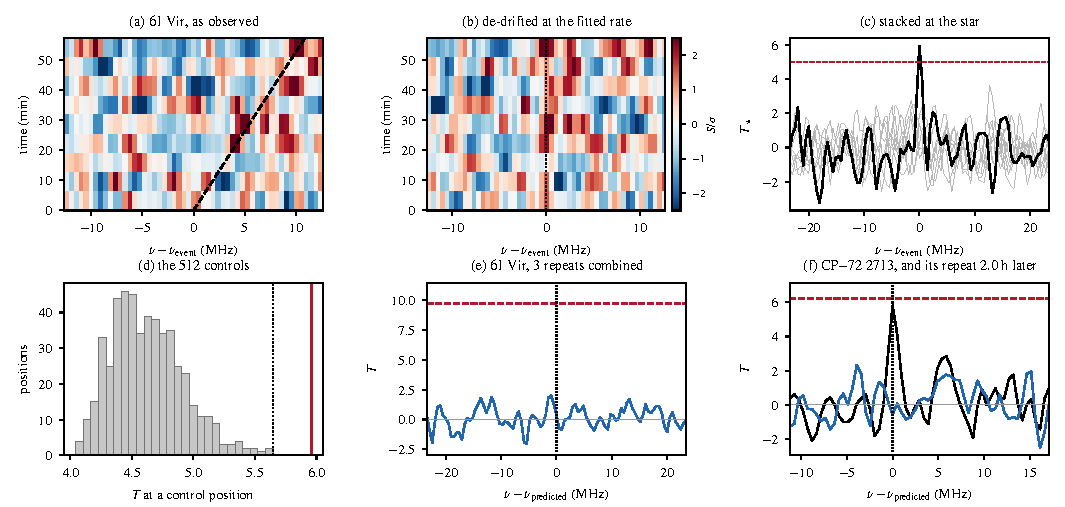
\includegraphics[width=\textwidth]{figures/event_crossings.pdf}
\caption{\textbf{Why this survey reports no confirmed signal although it
produced an interesting event.} \emph{(a)}~The dynamic spectrum at
\EvAStar's position around the crossing at \EvAFreq\,GHz, observed
\EvADate, with the fitted drift of \EvADrift\,Hz\,s$^{-1}$ as the dashed
track; the \EvANInt{} integrations are binned into \EvANBin{} and plotted in
units of each bin's noise. At \EvAFlux$\pm$\EvAFluxErr\,mJy against
\EvARmsInt\,mJy per integration the carrier is \EvAPerIntSig{} standard
deviations in any one of them and is invisible by eye, which is the point:
the event exists only in the \EvADwellMin-minute coherent stack.
\emph{(b)}~The same rows shifted by that drift, which carries the carrier
\EvADriftChan{} channels of \EvAChanwkHz\,kHz across the observation;
\EvANBinPos{} of the \EvANBin{} bins are positive at the marked channel.
\emph{(c)}~The de-drifted stack at the star (black) and at the
\RcNRetCtrl{} control positions with retained dynamic spectra (grey), in
units of its own noise; dashed, the trigger. \emph{(d)}~The same statistic
at each of the \NCtrl{} rank-screen control positions: the star reaches
\EvAT{} (solid) against a highest control of \EvACtrlMax{} (dotted).
\emph{(e)}~The \EvANRep{} other blocks covering that cell in the star's rest
frame, combined, with zero at the \emph{predicted} channel, which the frame
transport moves between epochs; the nearest is \EvANearH\,hours
\EvANearSign{} than the discovery (\EvARepDate), the farthest
\EvASpanD\,days. A persisting carrier would have returned $T=\EvATPers$
(dashed) against \EvATAnyDrift{} present, excluding it at \EvAExcl$\sigma$.
\emph{(f)}~The second event, \EvBStar{} at \EvBFreq\,GHz: its discovery
stack (black) and the same cell \EvBDeepH\,hours later in a block
\EvBDeepRatio{} times deeper (blue), where a persisting carrier would have
given $T=\EvBDeepTPers$ (dashed) against \EvBDeepTObs{} measured. The
inferred isotropic equivalent powers are
$\EvAEirp\times10^{\EvAEirpExp}$\,W at \EvADistPc\,pc and
$\EvBEirp\times10^{\EvBEirpExp}$\,W at \EvBDistPc\,pc.}
\label{fig:event}
\end{figure*}

\begin{table}
\centering
\caption{\textbf{The two events of Fig.~\ref{fig:event}}, the unattributed
crossings whose stellar statistic exceeds all \NCtrl{} control positions of
their own window. Repeat epochs measured are the blocks at which the
predicted stellar-frame cell was read; the indented rows give how many of
those the released catalogue carries and how many blocks it lists as
covering the frequency at all, which differ because the archival extension
is deposited separately. $T_{\rm rep}$ combines the repeat epochs by inverse
variance: it is one cell and one trial, so it may be negative, and it is the
quantity $T_{\rm pers}$ is compared against. The indented readings beneath it
are the largest single epoch and the largest over every drift trial, each a
maximum and so positive on average whatever is there. The exclusion is
$(T_{\rm pers}-T_{\rm rep})/\sqrt{1+(T_{\rm pers}/T_\star)^2}$, the
significance at which two readings of one amplitude disagree, and the last row
is the fraction of the discovery amplitude $S$ still ruled out at the trigger,
$(T_{\rm rep}+5)/T_{\rm pers}$. The radiated power quoted is that implied by
the flux in the peak channel; an unresolved carrier leaves only \HanMed{} of
its power there, so the power actually radiated is
$\times\HanFacBest$--$\times\HanFacWorst$ larger, a factor already inside
$\mathrm{EIRP}_{90}$ and not inside this row.}
\label{tab:cand}
\footnotesize
%% GENERATED by recur_v411.py -- do not hand-edit.
\begin{tabular}{@{}>{\raggedright\arraybackslash}p{0.49\columnwidth}@{~~}r@{~~}r@{}}
\hline
 & 61 Vir & CP$-$72 2713 \\
\hline
Frequency (GHz) & 346.313811 & 344.269746 \\
Channel width (kHz) & 488.28 & 488.28 \\
Drift rate (Hz\,s$^{-1}$) & $+3182$ & $-2056$ \\
$T_\star$ & 5.958 & 5.809 \\
Highest control $T$ & 5.65 & 5.68 \\
Flux density (mJy) & 118.8 $\pm$ 19.9 & 11.3 $\pm$ 2.0 \\
Peak-channel EIRP (W) & $5.1 \times 10^{14}$ & $8.9 \times 10^{14}$ \\
Repeat epochs measured & 3 & 5 \\
\quad in the released catalogue & 3 & 1 \\
\quad catalogue blocks at $\nu$ & 4 & 1 \\
Observed & 2017 May 20 & 2022 Oct 2 \\
Nearest covering epoch & 2017 May 19 & 2022 Oct 2 \\
\quad separation (h) & $-1.97$ & $+2.05$ \\
\quad covering epochs more than a day away & 2 & 4 \\
Longest baseline (d) & 3 & 2 \\
$T$ expected if persistent, $T_{\rm pers}$ & 9.70 & 6.30 \\
$T$ measured, matched drift, $T_{\rm rep}$ & +0.39 & -0.82 \\
\quad largest single epoch & +1.65 & +0.96 \\
\quad maximised over every drift & 2.71 & 3.60 \\
Exclusion, $\sigma_{\rm excl}$ & 4.9$\sigma$ & 4.8$\sigma$ \\
Amplitude still excluded at $5\sigma$ & 0.56 $S$ & 0.66 $S$ \\
Disposition & not confirmed & attributed \\
\hline
\end{tabular}

\end{table}

\begin{table*}
\centering
\caption{\textbf{The threshold crossings of the reserved hold-out}, searched
with the same frozen pipeline and disposed of by the same tests as the
census. $\Delta v_\star$ is the offset from the nearest masked transition in
the star's own frame and $n_{\rm rep}$ the number of covering repeat blocks;
$T_{\rm pers}$ and $T_{\rm rep}$ are as in Table~\ref{tab:ledger}. The one
crossing that is present again is a carbon monoxide line.}
\label{tab:holdout}
\scriptsize
%% GENERATED by holdout_v412.py -- do not hand-edit.
\begin{tabular}{@{}l@{~}l@{~}r@{~}r@{~}l@{~}r@{~~}r@{~}r@{~}r@{~}l@{}}
\hline
Star & block & $\nu_{\rm topo}$ (GHz) & $T_\star$ & line & $\Delta v_\star$ & $n_{\rm rep}$ & $T_{\rm pers}$ & $T_{\rm rep}$ & disposition \\
\hline
HD~285968 & Xdaef5a\_Xdd9b & 230.5081 & 8.642 & CO($2$--$1$) & +8.7 & 4 & 11.6 & +6.71 & attributed; present again \\
HD~14055 & X107376c\_X6126 & 330.7123 & 5.513 & $^{13}$CO($3$--$2$) & +112.6 & 30 & 312.0 & +0.56 & unattributed; does not recur \\
TRAPPIST$-$1 & Xd0e450\_X259b & 346.2454 & 5.326 & SO($9_{8}$--$8_{7}$) & -306.6 & 5 & 11.1 & -0.32 & unattributed; does not recur \\
HD~172555 & X107fa96\_X1300f & 344.6066 & 5.144 & SO($8_{8}$--$7_{7}$) & +251.3 & --- & --- & --- & unattributed; no repeat coverage \\
HD~285968 & Xdb4b9a\_Xa7c & 229.9129 & 5.106 & CO($2$--$1$) & -768.0 & 4 & 11.2 & +0.21 & unattributed; does not recur \\
HR~1010 & Xc6b674\_X23f2 & 346.2301 & 5.044 & SO($9_{8}$--$8_{7}$) & -238.7 & 7 & 25.9 & -0.80 & unattributed; does not recur \\
HD~10647 & Xff99e1\_X9cdf & 345.7059 & 5.017 & SO($2_{3}$--$2_{1}$) & +37.1 & 13 & 142.1 & -0.93 & attributed; does not recur \\
HD~170773 & Xff294f\_X1fb & 345.5597 & 5.001 & SO($2_{3}$--$2_{1}$) & -113.8 & 4 & 59.3 & +1.45 & unattributed; does not recur \\
\hline
\end{tabular}

\end{table*}

%% tab:ledger MOVED to Appendix D (sections/app_J_falsealarm.tex): a
%% full-width 56-row table* worth 0.72 pp of the main text.  Sec. 5.3 and
%% Sec. 5.6 carry the counts and cite it.



\begin{figure}
\centering
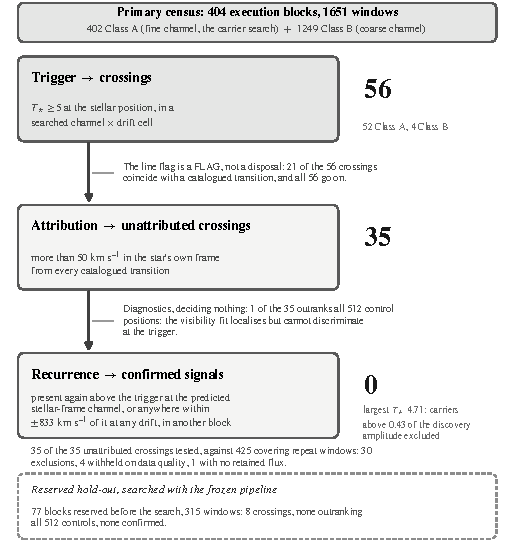
\includegraphics[width=\columnwidth]{figures/chain_v412.pdf}
\caption{The detection logic, with the count surviving each level. Three
levels and no more: a \emph{crossing} is an event requiring investigation, an
\emph{unattributed crossing} is a target for follow-up, and a \emph{confirmed
signal} would be a detection. Coincidence with a catalogued transition is a
flag and not a disposal, so all \CnCross{} crossings continue past it; the
spatial rank and the visibility fit are diagnostics attached to the middle
level and decide nothing. The reserved hold-out is drawn as a separate branch
because a transmitter in it would matter whatever its calibration role. Every
count is read from the ledger and the catalogue, so the figure,
Table~\ref{tab:ledger} and the text cannot disagree.}
\label{fig:chain}
\end{figure}

%% ---------------------------------------------------------------------
%% REQUEST (results owner -> numbers owner).  Eight macros this file uses
%% that the frozen layer does not yet define, all on the adopted
%% trigger-plus-spatial-screen criterion (EirpNinetyMultA = 5.70):
%%   \EirpNinetyWinMedA                      median Class A window, W
%%   \EirpNinetySysLoA \EirpNinetySysMedA \EirpNinetySysHiA
%%                                           per system, best window, W
%%   \EirpNinetyBarnLo \EirpNinetyBarnHi     Barnard's Star, W
%%   \EirpNinetyWolfLo \EirpNinetyWolfHi     Wolf 359, W
%% The \Promote* family (\PromoteMedA, \PromoteSysMedA, ...) is the same
%% quantity on the superseded localisation criterion and is cited nowhere
%% in this file; it is still cited in 03_sample.tex and 07_conclusions.tex,
%% which must move to the names above or the paper will carry two
%% sensitivities again.  \EirpBarnLo/\EirpBarnHi/\EirpWolfLo/\EirpWolfHi
%% are nominal triggers and are no longer quoted here.
%%
%% REQUEST (results owner -> numbers owner).  tab_ledger_v403 must drop
%% nine columns: both visibility-fit epoch groups (Re/sigma, Im/sigma,
%% ctrl, twice), the epoch displacement D, the off-channel column "off",
%% and the "scr" rank flag, whose result is carried by the disposition
%% code.  Eight columns remain: star, block, band, nu, T_star, line, dv,
%% disposition.  \LedgerLegend is replaced by the caption above, so the
%% legend macro is no longer referenced.
%%
%% REQUEST (results owner -> numbers owner).  tab_maskladder.tex now has a
%% home as Table tab:maskladder in this file.  Its fourth column header
%% reads "rank-flagged", a phrase this manuscript has used in both senses;
%% please rename it to "outrank all controls" so the header cannot be read
%% as its own opposite.  The caption states the meaning meanwhile.
%%
%% REQUEST (results owner -> figures owner).  fig:chain MUST BE RE-EMITTED
%% AT SINGLE-COLUMN GEOMETRY.  It is now a \begin{figure} at \columnwidth,
%% not a figure* at 0.98\textwidth, because the section measures 6.0 pp as
%% three full-width floats and 5.0 pp with this one in a column -- the
%% overage was float packing, not words.  chain_v403.pdf is still drawn for
%% full width, so its labels are currently at about half their intended
%% size: PLEASE RE-EMIT FOR ONE COLUMN.  A six-step vertical chain reads
%% better in a column than across a page, so this is the right geometry
%% for it, but the caption, the placement and the artwork must agree and
%% today only two of the three do.  If re-emission is refused, revert this
%% float to figure*/0.98\textwidth and the section is 6.0 pp.
%%
%% REQUEST (results owner -> figures owner).  fig:bpiccontrol.
%%  - GEOMETRY CONFIRMED SINGLE COLUMN.  bpic_control.pdf is 237.6 x 280.7 pt,
%%    i.e. one column wide with the two panels stacked vertically, and the
%%    float is \columnwidth in a \begin{figure}.  Caption and placement
%%    agree; no re-emission at full width is wanted.  Panel (b) gets the
%%    full column width this way, which is what it needs.
%%  - COUNTS I WOULD NOT INVENT.  \NStageOneBpicEb (9) counts the blocks in
%%    which the star outranks every control, so it cannot also count the
%%    points drawn: the ring-wins block is by definition not one of the 9.
%%    The caption therefore says "the 9 ... and one further block" rather
%%    than giving a total.  Four macros would let it say what is drawn:
%%      \BpicPanelNCo     beta Pic CO points in panel (b)        (10)
%%      \BpicPanelNOther  other crossings drawn in grey          (39)
%%      \BpicDvCoLo \BpicDvCoHi   |dv| range of the CO crossings (12-29)
%%      \BpicDvCsLo \BpicDvCsHi   |dv| of the two CS(5-4) crossings
%%    \BpicDvLo/\BpicDvHi existed earlier today and have since been retired.
%%  - COUNTEREXAMPLE NUMBERS, requested and still absent: the ring maximum
%%    (14.13), the stellar statistic (9.68) and the number of the \NCtrl
%%    controls above the star (6) in the ring-wins block.  When they exist
%%    the caption should name that block instead of gesturing at it.
%%
%% REQUEST (results owner -> integrator).  Labels and floats deleted from
%% this file, with the files that still reference them:
%%   sec:linecost     -> sec:bpicval   (06_discussion, app_F, app_I, app_K)
%%   sec:repairedstat -> app:v409      (08_backmatter, app_A, app_M)
%%   eq:tunif         no longer defined anywhere (app_L cites it)
%%   tab:crossdelta   float deleted with the revision-history material;
%%                    app_M_repaired.tex still cites it
%%   tab:clustv409    float deleted; nothing else cites it
%%   fig:ledgervis    no longer cited (float lives in app_K)
%%   tab:hosts        no longer cited from here
%%   app:etacrvrecur  no longer cited from here (app_M still cites it)
%% ---------------------------------------------------------------------
%
\subsection{A stellar-frame multi-epoch stacked search}
\label{sec:stack}

Combining the epochs of a star in that star's own rest frame deepens the
limit. \SxStkStarCensus{} of the surveyed stars, lying in \SxStkSysCensus{}
separate systems, hold more than one searched execution block. Over
\SyStkNGroup{} stacked groups, \SyStkNEpochComb{} epoch-windows and
\SyStkHours\,h, the flux limit improves by a median factor \SyStkGainMed{}
over each star's best single epoch and \SyStkGainMax{} at most.
\SxStkStarOutside{} further stars stack too --- \SyStkStarOos{} control stars
beyond 40\,pc and \SyStkStarOther{} covered only by archival blocks --- and
are left out of those figures; over all \StkNStar{} stacked stars the median
gain is \StkLimitGainMed, their stacks being shallow two-epoch ones. Every
stacked limit is measured by injection into the stack itself and never read
off a stacked spectrum as a threshold.

\emph{A fixed stellar-frame frequency is not a fixed observed frequency, so
the epochs are registered before they are added.} The barycentric term alone
swings by a median \StkVcorrSwingMed\,km\,s$^{-1}$ between the epochs of one
star and by as much as \StkVcorrSwingMax --- many channels at the
\StkRefChanKHz\,kHz Class~A width --- so epochs added as observed would dilute
rather than reinforce. Each epoch is transformed to the stellar rest frame,
divided by its own primary-beam response and combined by inverse variance
over the channels of common stellar-frame coverage, keyed on the star's
catalogued identity rather than the directory the search ran in. Spectra
whose archived visibility weights are pathological are excluded first
(\StkBadWeight{} of \StkNProd, which would otherwise dominate the sum). The transform is verified on a real line: HD~285968's molecular
line collapses from a \StkRegTopoChan-channel topocentric spread to
\StkRegStellarChan{} channels over \StkRegNEpoch{} epochs spanning
\StkRegSpanD\,d.

The criterion was fixed before any stellar position was examined: a stacked
$Z\ge\StkZmin$ above every stacked control maximum, no epoch supplying more
than \StkDomMax{} of the weighted sum, and at least \StkJkMin{} of the signal
surviving removal of the strongest epoch. Controls are stacked identically
and every clause evaluated at them, which measures the whole test's
false-alarm rate at \StkCtrlFap{} per cent against a \StkFapCeil{} per cent
ceiling fixed in advance.

\emph{The gain is $\sqrt{N_{\rm eff}}$ and not $\sqrt{N}$}, where
$N_{\rm eff}=\sigma_{\min}^{2}\sum_e\sigma_e^{-2}$ is the equivalent number of
equal-depth epochs and the median $N_{\rm eff}/N$ is \StkNeffFrac. What a
stack realises is $\sqrt{N_{\rm eff}}$ divided by the measured noise of its
own stacked spectrum, and that noise follows the inverse-variance prediction
to \StkGainVsNeff{} in the median, with a per-stack scatter of
\StkMadZScatterPct{} per cent and nine stacks in ten between \SzNoiseLo{} and
\SzNoiseHi, the sampling error of a noise scale measured over
\StkNChanMed{} channels. Against $\sqrt{N}$ the realised gain is \StkGainVsN, the
shortfall being unequal epoch depth, so an epoch count alone misleads.
\StkWorstStar{} stacks \StkWorstN{} epochs for a gain of only \StkWorstGain:
its $N_{\rm eff}$ is \StkWorstNeff, so $\sqrt{N_{\rm eff}}$ is
\SzWorstSqrtNeff, and its stacked spectrum came out \SzWorstNoise{} times as
noisy as predicted.

\emph{The deepest stacked limit is Proxima Centauri's, and it is a Class~B
limit.} Proxima is covered by \StkProxN{} blocks over \StkProxHours\,h
spanning \StkProxSpanYr\,yr, all of them coarse \ChanBModeMHz\,MHz windows,
so the stack constrains an unresolved spectral excess and discriminates no
drift. \SxProxEbCensus{} of those blocks belong to the primary census;
\SzProxEbSearched{} were searched afterwards from the same public archive and
\SzProxEbHold{} come from the reserved hold-out, and all of them were
observed over the same years as the census blocks themselves. Stacking the
census blocks alone, which is the set every other limit here is computed
over, gives $\mathrm{EIRP}_{90}=\SzProxEirpCensus$\,W; adding the rest of the
archive deepens that by \SzProxDeepen{} to $\StkProxEirpCal$\,W, against
$\StkProxEirpSingle$\,W for the best single epoch on the same
injection-calibrated convention. Its $N_{\rm eff}$ is only \StkProxNeff, so
$\sqrt{N_{\rm eff}}=\SxProxSqrtNeff$ of the measured \StkProxGain{} is what
combining the epochs buys, the rest being this spectrum's own noise,
\SyProxNoiseMeas{} of prediction over \SxProxNChan{} channels. The limit
holds for an emitter steady in the
stellar frame to within one \ChanBModeMHz\,MHz channel,
\StkProxTolKms\,km\,s$^{-1}$ peak to peak, with no inter-epoch drift above
\StkProxDriftHzS\,Hz\,s$^{-1}$. At \StkProxDistPc\,pc that depth is mostly
geometry; the gain is what stacking bought.

\emph{\StkNSurvive{} groups pass the full criterion and both are known
lines.} They are $\beta$~Pictoris' CO $J=1\!-\!0$ at
\StkBpCoOneOff\,km\,s$^{-1}$ over \StkBpCoOneN{} epochs ($Z=\StkBpCoOneZ$)
and its $J=2\!-\!1$ at \StkBpCoTwoOff\,km\,s$^{-1}$ ($Z=\StkBpCoTwoZ$),
agreeing to \StkBpCrossKms\,km\,s$^{-1}$ or \StkBpCrossChan{} of a CO(1--0)
channel: the astrophysical positive control passing in the stack. The
survey's own $\pm\StkAttrKms$\,km\,s$^{-1}$ mask leaves
\StkNUnattributedComputed{} of them unattributed. The stack is also an independent test of the threshold
crossings of \S\ref{sec:etacrv}: the \StkNPersistStar{} stars carrying them
stack to $Z=\StkPersistZLo$--\StkPersistZHi{} in \StkNPersistBelow{} cases,
\StkNPersistAboveCtrl{} exceed their own control ensembles and
\StkNPersistSurvive{} passes the criterion. The exception,
\StkPersistLineStar, reaches $Z=\StkPersistLineZ$ on the foreground line
used above as the registration standard and is rejected because its own
controls reach \StkPersistLineCtrl: the emission is extended, as a cloud is
and a transmitter is not.

\emph{The restriction travels with every number above, and its width is the
channel.} At CO(2--1) one \StkRefChanKHz\,kHz channel spans
\StkTolFineKms\,km\,s$^{-1}$, and that is the whole excursion a stacked
carrier is allowed, peak to peak. A transmitter on a short-period giant
planet, whose line-of-sight velocity swings by
$\pm\StkReflexAmpKms$\,km\,s$^{-1}$, crosses \SzReflexPPChanFine{} of those
channels peak to peak and so de-registers itself completely, against
\SzReflexPPChanCoarse{} channels of a \ChanBModeMHz\,MHz window: the coarse
stacks buy reflex tolerance with bandwidth. Drift divides the same way, a
stack in \StkRefChanKHz\,kHz channels being confined to
\StkDriftTolHzS\,Hz\,s$^{-1}$ over the median inter-epoch span of
\StkSpanMedD\,d. Each stacked limit therefore constrains only emitters
stable in the stellar frame to within its own channel; the single-epoch
limits of \S\ref{sec:excludes} apply generally.
%
\section{Discussion}
\label{sec:discussion}

\subsection{What is different about a millimetre technosignature search}
\label{sec:mmdifferent}

The most transferable result of this experiment is not the non-detection but
a measurement of what limits a carrier search at these wavelengths. For
classifying a crossing in the present archival data set, molecular-line
confusion and sparse repeat coverage are more immediate limitations than
thermal sensitivity. That is a statement about disposing of events and not
about depth: the power a transmitter must radiate to be found here remains a
median $\EirpNinetySysMedA$\,W per system.

\emph{Confusion, and not interference, sets the false-positive rate.}
Catalogued molecular transitions, almost all of them carbon monoxide, account
for \NAttributed{} of the \NCross{} threshold crossings, and no crossing in
this survey is attributed to interference (Appendix~\ref{app:rfi}).
\DiscFpWin{} of the \DiscFpOfFlags{} windows that reached the spatial stage
are disc or foreground carbon monoxide, arising in \DiscFpSys{} of the
\NDebrisKwSys{} debris-disc systems searched. The remedy that works is a
velocity-space mask evaluated in the stellar frame, and it is not free: it
removes \FrMaskPct{} per cent of otherwise usable coverage.

\emph{Spatially extended emission is the second discriminant, and it has no
analogue at centimetre wavelengths.} A line filling the primary beam raises
the star and the control annulus together instead of cancelling, so the
spatial statistic loses power exactly where circumstellar gas is brightest.
$\beta$~Pictoris shows the benign face: the frozen pipeline recovers its
circumstellar carbon monoxide blind, in two transitions, which is the positive
control the experiment needed. HD~48370 shows the other. Its resolved disc
emission lies near a band edge, and that one window contributes
\VnEdgeDomPct{} per cent of every near-edge threshold exceedance in the
survey: pooled, the near-edge rate is $\times\VnEdgeRatio$ the interior rate;
without that window $\times\VnEdgeNoDomRatio$, and on a held-out half
$\times\VnEdgeHalfCleanRatio$ ($\pv{\VnEdgeHalfCleanP}$). What looked like a
property of band edges is one disc, so no edge correction is applied to any
limit.

\emph{The channelisation is inherited.} \NCoarse{} of the \NWindows{} windows
have channels so coarse that every drift in the grid stays inside one channel
over a whole track; they measure an amplitude but cannot distinguish a
drifting carrier from a stationary one, which is why the carrier search rests
on \NWinA{} of them. The widths on offer here run from
\SzChanFinestKHz\,kHz to \SzChanWidestMHz\,MHz, about \SzChanDexSurvey{}
orders of magnitude; set beside the \SzChanLitHz\,Hz channels of
centimetre-band carrier searches the range becomes \SzChanDexAll{} orders
(Fig.~\ref{fig:context}(b)), and nothing in the search could choose them.

\emph{Repeat epochs turn a crossing into a testable claim, and an archive
supplies them only incidentally.} Let the \emph{confirmation coverage}
$C_{\rm conf}(\nu)$ be the number of systems toward which two independent
execution blocks more than a day apart both cover the sky frequency $\nu$, so
that a carrier found once there could have been sought again. It must be
stated against frequency rather than as a fraction of the sample, because
repeat visits re-tune and a second epoch is of no use at a frequency it does
not cover. Its support is \CvConfGHzDay\,GHz of union bandwidth,
\CvConfPctDay{} per cent of the \CvUnionA\,GHz searched, falling to
\CvConfGHzYr\,GHz beyond a year, and at its best near \CvConfNuMaxDay\,GHz it
reaches \CvConfNMaxDay{} systems (Fig.~\ref{fig:confcov}). The searched extent
is about twice the extent over which a persistent carrier could have been
confirmed, and for close to half the sample the archive constrains an
intermittent emitter hardly at all, whatever its power.

\begin{figure}
\centering
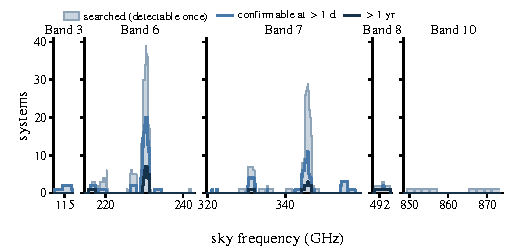
\includegraphics[width=\columnwidth]{figures/confcoverage.pdf}
\caption{What could be searched against what could be confirmed. For the
Class~A experiment, against sky frequency: the number of systems toward which
a carrier could have been detected once (grey), the number for which a second
independent execution block more than a day later also covers that frequency
(blue), and the same beyond a year (dark). One panel per populated ALMA band,
widths in proportion to the frequency each contributes, as in
Fig.~\ref{fig:covmap}.}
\label{fig:confcov}
\end{figure}

\emph{Finally, a threshold is not a sensitivity.} A trigger level is a
property of the noise, not of what a transmitter of a given power does to a
pipeline: measured by injection and recovery through the unchanged selection,
the power needed for ninety per cent recovery is $\EirpNinetyMultA$ times a
Class~A window's own trigger power and $\EirpNinetyMultB$ times a Class~B
window's.

\subsection{The search space this archive opens}
\label{sec:newspace}

The carrier search is \NWinA{} fine-channel windows toward \NSysClassA{}
stellar systems, \CvUnionA\,GHz of union bandwidth; the \NWinB{}
coarse-channel windows are a supplementary spectral-excess experiment. No previous search has looked for
technosignatures toward stars within 40\,pc at any frequency above about
30\,GHz, and the one earlier millimetre search worked in Band~3 toward far
more distant stars (\S\ref{sec:background}), so Band~3 is
not searched toward nearby stars either. \UnionBandThree\,GHz of the union here lies inside the 10\,MHz--115\,GHz
interval \citet{Wright2018} adopt as the frequency axis of the search
haystack.

Union bandwidth alone overstates what that buys: different frequencies were
searched toward different numbers of stars and to very different limits. Figure~\ref{fig:covmap} therefore gives the quantity a
reader needs instead: how many independent systems would have yielded a
recovery at ninety per cent completeness, against sky frequency and
transmitter power. At an
EIRP of $\CovEirpRefTex$\,W the covered frequency falls to
\CovUnionAtRef\,GHz, \CovFracAtRef{} per cent of the union, reaching
\CovNSysAtRef{} systems in all and \CovNMaxAtRef{} at the best-covered
frequency near \CovNuMaxAtRef\,GHz; with no limit on power that frequency
reaches \CovNMaxFull{} of the \NSysClassA{} systems, and half the sample
only above $\CovEirpHalf$\,W.

\begin{figure}
\centering
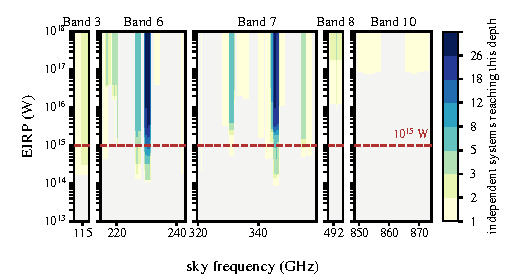
\includegraphics[width=\columnwidth]{figures/completeness_map.pdf}
\caption{Where the experiment could have found something. Shading gives the
number of independent systems that would have yielded a recovery at 90 per
cent completeness for an unresolved carrier of the plotted EIRP at the
plotted sky frequency; unshaded means none. One panel per populated ALMA
band, with panel widths in proportion to the frequency each contributes: the
\CvUnionA\,GHz Class~A union is \CovNIslands{} disjoint islands across
\DomAFreqLo--\DomAFreqHi\,GHz, which a continuous abscissa would draw as
hairlines. The dashed line is $\CovEirpRefTex$\,W.
Figure~\ref{fig:waterfall} shows where ALMA looked; this shows where the
experiment was sensitive.}
\label{fig:covmap}
\end{figure}

\emph{Archival SETI buys sky and frequency cheaply and buys confirmation not
at all.} Across both classes this experiment reached \NSystems{} systems and
\UnionGHz\,GHz of union bandwidth without an allocation, on data selected
by others and therefore with the biases of \S\ref{sec:bias}.

For comparison with other programmes the conventional measure is the
continuous-waveform transmitter figure of merit of \citet{Enriquez2017},
$\mathrm{CWTFM}=\zeta_{\rm AO}\,\mathrm{EIRP}_{\rm min}/
(N_{\star}\nu_{\rm rel})$ with $\nu_{\rm rel}=\Delta\nu/\nu_{\rm mid}$,
smaller being better. Those programmes quote $\mathrm{EIRP}_{\rm min}$ at a
bare detection threshold, so this one is put on the same footing: for the
Class~A experiment, with $N_{\star}=\NSysClassA$ and
$\nu_{\rm rel}=\FomNuRel$, it is $\SzCwtfmBareWorst$ on the sample's largest
threshold power and $\SzCwtfmBareMed$ on the median system, against
\FomLitEnriquez{} for \citet{Enriquez2017}. \citet{Margot2023} publish no
CWTFM; evaluating the same expression on the three quantities they do give
--- \FomMargotN{} stars, \FomMargotLo--\FomMargotHi\,GHz and
$\mathrm{EIRP}>\FomMargotEirp$\,W --- returns \FomLitMargot.
Carried through instead with the $\mathrm{EIRP}_{90}$
adopted everywhere else here, the same two become $\FomCwtfmWorst$ and
$\FomCwtfmMed$. Nearly all of
the difference is the product $N_{\star}\nu_{\rm rel}$: this is a far smaller
haystack than a wideband centimetre survey of thousands of stars, and the
measure compares surveys rather than estimating an occurrence rate.

\subsection{What this experiment excludes, and what it does not}
\label{sec:excludes}

\noindent\emph{Excluded.} Consider a continuously transmitting, unresolved
carrier that lies outside the molecular-line mask, inside the searched
frequency range and inside the linear-drift grid, and that is present during
one of the archival epochs. Such a carrier would have been found nine times
in ten above the $\mathrm{EIRP}_{90}$ of \S\ref{sec:pninetysel}, a median of
$\EirpNinetySysMedA$\,W per system on its best window. None is present toward
any of the \NSysClassA{} systems the carrier search covers.

Four further axes bound the excluded population as sharply as power does.
\emph{Frequency:} the coverage is sparse and inherited (Fig.~\ref{fig:covmap})
and the median system is covered over only \SysUnionAMed\,GHz. \emph{Drift and
acceleration:} the grid reaches a line-of-sight acceleration of
\AccelCeilMed--\AccelCeilMax\,m\,s$^{-2}$, which contains every known planet
of the sample but one (Fig.~\ref{fig:accel}); an oscillator drifting faster
than that lies outside it. \emph{Persistence:} the carrier must be radiating
during one of the archival observations. \emph{Spectral width:} the statistic
is built for emission confined to one \ChanLoA--\ChanHiA\,kHz channel, and
anything broad enough to resemble continuum is removed with the spectral
baseline.

\noindent\emph{Not excluded.} A transmitter absent during the archival
observation, or on for much less than the length of one. The limits scale
inversely with the duty cycle (\S\ref{sec:pninetysel}), so a carrier
radiating a tenth of the time is constrained only at $\DutyPowFac\times$
the powers quoted here, and because the intermittency trials carry no drift
the joint drifting and intermittent case is not measured at all. Emission inside the
$\pm\MaskHalfKms$\,km\,s$^{-1}$ molecular-line mask, at any strength, which
costs \FrMaskLostGHz\,GHz of union bandwidth. Drift outside the searched grid, or
drift curved enough to leave a channel within the track. Signals broad enough
to be removed with the continuum baseline. Anything below a window's own
completeness. And any emission from the \NGaiaCensus{} stars within 40\,pc
that ALMA has not observed, which is almost all of them.

\noindent\emph{An illustrative engineering benchmark.} A \BenchDiam\,m dish
radiating \BenchPowerMW\,MW at \BenchFreqGHz\,GHz with an aperture efficiency
of \BenchEta{} has a directive gain $G=\eta(\pi D\nu/c)^{2}=\BenchGain$ and so
an EIRP of $\BenchEirp$\,W, a depth this survey reaches for \BenchNSysA{} of
the \NSysClassA{} Class~A systems. The same gain fixes how narrow the beam is,
and detection requires the Earth to lie inside it: a solid angle
$\Omega=4\pi/G=\BmOmegaSr$\,sr, about \BmArcsec{} arcsec across, illuminating a
fraction $\Omega/4\pi=\BmSkyFrac$ of the sky at a time. The example shows that EIRP is not transmitter power --- the
same megawatt radiated isotropically would be $10^{6}$\,W --- so these limits
apply to beamed transmitters whose beam contains the Solar System and say
almost nothing about omnidirectional beacons.

\noindent\emph{Two blind spots.} The search is Stokes~$I$ only, so the
discrimination that polarisation would offer against unpolarised
astrophysical emission is unavailable; ALMA's feeds are linear, and the
circularity of a circularly polarised carrier lies in the cross-hands, which
this analysis does not extract. And the frequency coverage is the archive's
and not a choice: none of the ``magic frequency'' arguments that have guided
centimetre-band searches falls in an ALMA band, so a transmitter deliberately
placed on one lies outside this experiment by construction.

\subsection{What a dedicated ALMA technosignature experiment should do
differently}
\label{sec:future}

A purpose-built experiment on the same telescope would be far stronger, and
the changes it needs follow from the limitations above. \emph{Channelise
finely everywhere:} the \NCoarse{} coarse-channel windows measure an amplitude
but cannot distinguish a drifting carrier from a stationary one.
\emph{Choose the targets and the frequencies:} an archive weighted toward
dusty discs is the worst case for molecular-line confusion, the M~dwarfs that
dominate the nearby habitable-zone planet census are the least covered, and
windows placed deliberately away from the bright transitions would recover
most of the \FrMaskLostGHz\,GHz the mask costs --- all three are decisions a
proposal can simply reverse. \emph{Repeat the epochs on purpose, at the same
tuning:} two or three visits separated by days and by years turn a crossing
into a testable claim, and the separation is a scheduling constraint rather
than extra sensitivity; Fig.~\ref{fig:confcov} is what its absence costs.
\emph{Retain the visibilities:} rotating the phase centre to the star leaves a
genuine point source entirely in the real part of the visibility. That asks
whether the data contain a source \emph{where the star is}, which is a
stronger question than any rank
against neighbouring positions in an image.

%% ---------------------------------------------------------------------
%% REQUEST (06_discussion owner -> integrator). Consequences of this pass.
%% None of them is in a file I own; each is also written up as a numbered
%% entry in referee_r10/INTEGRATION_QUEUE.md.
%%
%% Q1. LABELS. sec:newspace, sec:excludes and sec:discussion are unchanged.
%%     sec:exposure and sec:parallax are GONE (see Q2, Q3); no file refers
%%     to either. sec:lessons is renamed sec:mmdifferent; the benchmark is
%%     a labelled paragraph inside sec:excludes, which is where \S2 now points.
%% Q2. THE OMITTED ANNUAL PARALLAX subsection is deleted from the Discussion
%%     under the ruling that the correction is applied rather than stated.
%%     The statement must now be made exactly once, where it is applied, in
%%     Section 5.1 / Appendix A. Macros \PxNWin, \PxLossMedPct,
%%     \PxLossMaxPct, \PxNGtTen and \PxNSysCorr are no longer referenced by
%%     any file I own and retire_macros.py will drop them unless that
%%     statement cites them.
%% Q3. THE ON-SOURCE TIME subsection (two offsetting bookkeeping biases) is
%%     deleted here as reproducibility detail. It belongs in Appendix A.
%%     Macros \TruncNBlocks, \ExpNBlocks, \TruncNWin, \TruncNStars,
%%     \TruncHoursLost, \TruncPctSurvey, \TruncGainMed, \OcOldMax,
%%     \OcNewMax, \ExpNetLo, \ExpNetHi are orphaned by that deletion.
%% Q4. THE MASON MATCHED-RECEIVED-FLUX COMPARISON is now made once, in
%%     Section 2, as that section's own request asked. \FluxSelMatchMed and
%%     \FluxSelMedRatio are unused.
%% Q5. THE BENCHMARK must stop being quoted as a headline result elsewhere:
%%     it is now an explicitly illustrative example in Section 6.3.
%%     Remove it from the abstract, from Section 5 and from conclusion 3,
%%     each of which should quote the EIRP_90 limit alone.
%% Q6. CONCLUSION 1 states that \UnionBandThree GHz of the searched range
%%     lies inside the interval covered by centimetre-wave programmes. It
%%     does not; that is the Band 3 union inside the Wright et al. haystack
%%     AXIS. Replacement text is in the integration queue.
%% Q7. Figure fig:covmap is new and is paid for: the millimetre-motivation
%%     paragraph (duplicated from Section 1), the Mason flux comparison, the
%%     parallax subsection and the exposure subsection are all deleted here.
%% ---------------------------------------------------------------------
%
\section{Conclusions}
\label{sec:conclusions}

\begin{enumerate}[leftmargin=1.6em,itemsep=4pt,topsep=4pt,parsep=0pt]

\item The frequency range is what makes this experiment new: no published
radio technosignature search above about 30\,GHz has reached a star within
40\,pc (\S\ref{sec:background}), and an archive assembled for other science
is at present the only way to reach one.

\item The primary experiment is \NWinA{} fine-channel windows toward
\NSysClassA{} stellar systems, covering \CvUnionA\,GHz of union bandwidth in
disconnected intervals, searched for an unresolved carrier whose frequency
drifts. A supplementary coarse-channel search for an unresolved spectral
excess adds \NWinB{} windows toward \PrSysClassB{} systems and
\CvUnionB\,GHz of union bandwidth, with no drift discrimination. Both come
from one uniform reduction of \NEB{} public execution blocks,
\TotalDataTB\,TB of raw data, and between them they span
\SurvFreqLo--\SurvFreqHi\,GHz.

\item Sensitivity is a measured completeness, not a threshold. Carriers
injected into the real calibrated visibilities are recovered through the
unchanged selection --- the trigger, and localisation at the star --- and
$\mathrm{EIRP}_{90}$ is the power at which nine in ten come back. The median
system's best window reaches $\EirpNinetySysMedA$\,W, with a spread across
systems of $\EirpNinetySysLoA$--$\EirpNinetySysHiA$\,W. The rank and the
visibility fit decide nothing, so neither is charged to that limit. One bias
runs one way only and is not inside the quoted calibration: an injected
carrier suffers no atmospheric decorrelation where a real one would, so
every limit here is optimistic by up to \SensDecorPct{} per cent.

\item All \EvNCrossRaw{} threshold crossings are reported with their
dispositions, \PrFlagXrossWord{} of them in the one execution block
that fails the data-quality criterion of
Appendix~\ref{sec:blockquality} and reported apart from the
\EvNCrossQp{} in quality-passing data; of those, \EvNAttrQp{} coincide with
a catalogued molecular transition, almost all of them carbon monoxide ---
including the $\beta$~Pictoris disc, which the search recovered without
being told where to look --- and \EvNUnattrQp{} do not.

\item Every unattributed crossing was tested for recurrence in the star's
own frame, in each further execution block covering the event frequency and
over the whole of each such window at every drift searched, because a
carrier on an accelerating platform need not return to one channel. None is
present again: the largest statistic at any predicted cell is \RcTMax{}
against $T_{\rm trig}=\StageNullTrig$, and the exceedances found anywhere in
those windows are no more than chance predicts for trials of that size.
Where a discovery amplitude survives, the repeat coverage rules out a
carrier of that amplitude in \RcNExcl{} cases, and one of half that
amplitude or less in \RcNFracHalf{} of them; taken instead as a
disagreement between two measurements of the same amplitude, discovery and
repeat differ by \RcExclMin{} to \RcExclMax$\sigma$, median
\RcExclMed$\sigma$, which is as much as the pair can say when the discovery
amplitude is itself a five-sigma measurement. Nor did \PrRankClause{}
return. What these tests exclude is a carrier that holds its frequency
inside the window searched and radiates through both observations, and not a
persistent transmitter of any kind.

\item What this survey could search and what it could confirm are different
extents. The carrier search covered
\RcSearchSys{} systems, of which only \RcConfSysDay{} --- carrying
\CvConfPctDay{} per cent of the searched union bandwidth --- were observed
again at the same frequency more than a day apart, and \RcConfSysYr{} beyond
a year. Across both classes, \RcNoRepSysAll{} of the \RcSearchSysAll{}
systems have no second block covering a frequency the first one covered, and
toward those the null reported here says nothing at any strength.

\item Combining each surveyed star's epochs in its own rest frame deepens
the flux limit by a median factor \SyStkGainMed. For Proxima~Centauri,
where $\sqrt{N_{\rm eff}}=\SxProxSqrtNeff$ is what combining the epochs
buys, the stacked limit measured by injection into the stack reaches
$\SzProxEirpCensus$\,W over the primary census alone and
$\StkProxEirpCal$\,W once the rest of the archive is added, in
\ChanBModeMHz\,MHz channels --- a Class~B limit on an unresolved excess,
carrying no drift discrimination --- for an emitter steady in the stellar
frame to within one channel, \StkProxTolKms\,km\,s$^{-1}$ peak to peak,
across \StkProxSpanYr\,yr.

\item These results constrain unresolved carriers only within the domain
actually searched and only toward this archive-selected sample
(\S\ref{sec:excludes}). What transfers beyond it is the obstacle: a
channelisation chosen by other observers for other purposes, and not
collecting area, is what decides which kind of search is possible at all.

\end{enumerate}
%
\section*{Author contributions}
G.J.W.\ conceived the survey, defined the target sample and the selection
criteria, and wrote the manuscript. R.D.\ built and operated the archival
retrieval, calibration and search pipeline, implemented the spatial control
statistic and the injection--recovery campaigns, and produced the released
catalogue and its regeneration scripts. Both authors designed the vetting
procedure, chose the masked species, carried out the statistical
validation reported in \S\ref{sec:statistic} and
Appendix~\ref{app:falsealarm}, and agreed the dispositions of
Table~\ref{tab:ledger}.
%% AUTHORS: confirm this division before submission, and see
%% AUTHOR_ACTIONS.md item 6 for the affiliation statement this section
%% should be read with.

\section*{Funding}
This work received no dedicated funding. It used public archival data and
no observing time was awarded for it.
%% AUTHORS: replace if any grant supported this work.

\section*{Competing interests}
The authors declare no competing interests. VBRL Holdings is a privately
held company through which R.D.\ conducts independent research, named
here solely as his affiliation; it had no role in the design of the
survey, the selection of targets, the analysis, the decision to publish
or the content of this paper, and provided no funding for the work.
%% AUTHORS: confirm this wording, which is written to be accurate only if
%% the company's involvement was indeed nil. See AUTHOR_ACTIONS.md item 6.

\section*{Acknowledgements}
This paper uses ALMA data from the public ALMA Science Archive. The \NEB{}
primary-census execution blocks searched span 2013 October~6 to 2025
June~11 and belong to \NProjCodes{} ALMA proposals, whose codes, in the
standard ADS/JAO.ALMA\#\textit{code} form, are recorded block by block in
the data release together with each block's
epoch.\ProjCodeUnresClause{} ALMA is a partnership of ESO
(representing its member states), NSF (USA) and NINS (Japan), together with NRC
(Canada), NSTC and ASIAA (Taiwan), and KASI (Republic of Korea), in cooperation
with the Republic of Chile. The Joint ALMA Observatory is operated by ESO,
AUI/NRAO and NAOJ. This work has made use of data from the European Space
Agency (ESA) mission {\it Gaia} \citep{GaiaDR3}, processed by the {\it Gaia}
Data Processing and Analysis Consortium (DPAC). This research has made use
of the SIMBAD database (CDS, Strasbourg, France), of the NASA Exoplanet
Archive \citep{NEA2013}, and of the Splatalogue spectral-line database
\citep{Splatalogue2007}.

\section*{Data Availability}
\label{sec:data}
The reference of record is a single permanent Zenodo deposit, cited by its
DOI. It carries every number in this paper and the code that produced them,
and contains: the \NStars-star target catalogue with its selection
function; one row for each of the \NWindows{} searched windows, carrying
its execution-block identifier, frequency limits,
native channel width, trial-drift grid, trigger statistic at the stellar
position, control statistics of the \NCtrl-position ring and the window's
$\mathrm{EIRP}_{90}$; the ALMA proposal code and epoch of every execution
block, so that each of those rows resolves to the programme that took it;
all \EvNCrossRaw{} threshold crossings with their
stellar-frame frequencies, line classifications, recurrence measurements
and dispositions; the search statistic and the molecular-line list as files
in their own right; the injection--recovery records; the block-by-block
archival verdicts and the ALMA delivery record for every block in scope
that could not be searched; the diagnostic figures the printed paper refers
to but does not reproduce, among them the per-system coverage waterfall and
the selection funnel (\texttt{coverage\_waterfall\_full.pdf},
\texttt{selection\_funnel.pdf}); the illustrative table of sample systems
within 15\,pc with a confirmed planet; and the full pipeline with the
commit that produced the deposited products. Two properties of the deposit are
measured rather than claimed: \NRegenProducts{} generated products
regenerate byte-identically from the frozen inputs, and \NReproChecks{}
headline quantities are re-derived from the released catalogue alone,
without the pipeline.

Three of the choices that could create or remove an unattributed crossing
carry an identifier that can be checked independently of the deposit. The
calibration hold-out rule of Appendix~\ref{sec:heldout} and the block list
its first guard depends on were committed to the project repository as
\texttt{c75069040eab52ec1336376a4dae62114bb281a3} on 2026 September~14 at
07:10~UTC, \HoLeadBlockDays{} days before the first reserved block was
searched. The molecular-line list is a single dated query of a public line
catalogue (\McQueryDate) deposited as a file, so it is reproducible rather
than described; it post-dates the fixing of the disposition criteria on
\MkCritDate{} (\texttt{f5f52e7804f1baad99515ea2d46ddd7e4e4cd546}), and so
does every species in it, which is why the same rule is applied to all of
them and no species is withheld from one coincidence and allowed in another
(Appendix~\ref{app:linemask}). The repository at
\url{https://github.com/Tilanthi/SETI} is a working mirror and may move on.
%% AUTHORS -- THREE BLOCKERS, in AUTHOR_ACTIONS.md items 1, 2 and 10.
%% (1) Reserve the Zenodo DOI and insert it in the first sentence above.
%%     `python3 doigate.py` FAILS until a real, non-placeholder DOI is
%%     there, and it also fails if the inventory above is lost; run it
%%     before submission.  It is deliberately NOT in make_all.sh, because
%%     a gate that blocks every build gets switched off.
%% (2) Create a Zenodo private reviewer link and put it in the cover
%%     letter: a DOI minted at acceptance cannot be checked during review.
%%     It is not promised in the text above, because the text may not
%%     claim it before it exists.
%% (3) Tag the submitted commit and name the tag in the deposit, so "the
%%     commit that produced the deposited products" resolves.
%% Item 10 also records what a dated timeline of the fixed choices would
%% need before it could be printed: three of the four rows now carry a
%% verifiable identifier, the search statistic still does not.

\section*{Software}
The pipeline depends on CASA~6.7.6 \citep[casatools/casatasks
6.7.6-14;][]{CASA2022}, Python~3 with astropy \citep{Astropy2022}, numpy
\citep{Harris2020} and scipy \citep{Virtanen2020}, and the ALMA Science
Archive and SIMBAD TAP interfaces through astroquery \citep{Ginsburg2019};
all are free and open-source, with exact
versions recorded in the frozen release.
%
\appendix

%% APPENDIX A -- spectral response, frequency conventions, primary-beam response.
%% Owner: appendix-triage.  Carries \label{app:conventions} (cited by
%% 04_method.tex) and \label{app:pbresp}.
\section{Spectral response, frequency conventions and the primary-beam
response}
\label{app:conventions}

Checking a threshold in this paper needs three things: the frame every
frequency is quoted in, the instrumental response that separates a channel
threshold from a transmitter power, and the primary-beam factor that turns a
measured noise into a flux at the star. The per-window catalogue,
\texttt{catalogue/windows.csv} in the deposit, carries the columns each of
them uses.


%% The single-column figure that plotted the three-point Hanning response
%% against sub-channel phase has been removed: it illustrated an analytic
%% kernel whose every number is now in the paragraph on the peak-channel
%% fraction below, and it was worth a whole typeset page against a hard
%% length limit.  See queue/QUEUE_integrate.md entry S6: make_all.sh must
%% stop running make_fig_hanning.py and figorphan.py must carry
%% hanning_response.pdf in PENDING, or the figure gate fails.

\subsection{Frequency frames, linewidth and smearing}
%% (subsection label retired: nothing cites it)

Every frequency axis here --- searched spectra, tabulated ranges and
crossing frequencies alike --- is \emph{topocentric} as delivered by the
ALMA correlator, and the search itself applies no velocity-frame shift.
Velocities enter at the vetting stage, where the line mask is evaluated in
each star's own rest frame: it carries every crossing frequency to the
barycentre at its own block's epoch and then to the stellar frame before
comparing it with a transition (Appendix~\ref{app:linemask}). The residual
error is then the catalogue radial-velocity uncertainty alone, a few
km\,s$^{-1}$ within 40\,pc; second-order relativistic terms at the
\MaskHalfKms\,km\,s$^{-1}$
scale are $\lesssim5$\,kHz at 350\,GHz, below the finest native channel
searched. The stacking is drift-aligned and inverse-variance weighted:
coherent in frequency trajectory, not in electric-field phase.

The native channel width is also the linewidth convention for every EIRP
threshold. The statistic is the single-channel flux density after drift
correction, so EIRP$_{\rm trig}$ is the minimum \emph{total} power of a
channel-confined carrier, flat in the assumed linewidth below the channel and
never a spectral power density; flatness is exact only for a centred tone,
and a boundary-straddling one divides its power between two channels, which
is the loss the injections carry and one reason EIRP values are quoted to two
significant figures. The Hz-resolution
surveys' limits are total powers in the same sense, each the best case of
its own channelisation, which makes the axes of Fig.~\ref{fig:context}(a)
commensurable. One number fixes the scale, illustratively and not
achievably: rechannelising the median Class~A window's
\SqrtScaleChanKHz\,kHz to the \SETIChanHz\,Hz of a dedicated narrowband
search would divide the threshold by $\SqrtScaleFac$, and no reprocessing
recovers resolution the correlator never recorded.

Channel widths come from the measurement sets' own CHAN\_WIDTH; MS~v2
defines no ``EFFECTIVE\_BANDWIDTH'' column, so the quoted channelisations are
separations and are not claimed to be noise bandwidths.

ALMA applies online Hanning smoothing by default \citep{ALMAHandbook}, so
the spectral response is ${\sim}2$ channels wide and neighbouring channels
are correlated. For the $0.25/0.5/0.25$ kernel the coefficients
are $\rho_1=\HanRhoOneFrac=\HanRhoOne$ and $\rho_2=\HanRhoTwo$, with
$\sigma_{\rm smoothed}/\sigma_{\rm raw}=\HanSigRatio$: the correlation is
not confined to adjacent channels, the lag-two term being a sixth. The peak
channel holds \HanBest{} of an unresolved carrier's flux at a channel centre
and \HanWorst{} on a boundary, a median \HanMed{} over sub-channel phase, so
a nominal threshold is optimistic by
$\times\HanFacBest$--$\times\HanFacWorst$; the released catalogue carries the
nominal threshold and both corrected values for every window.

\emph{The injected carriers are deposited with the correlator's own channel
response, at a sub-channel phase drawn afresh for each tone, so the smoothing
loss sits inside the measured completeness rather than being applied to it.}
The deposited profile is the tone divided between the two channels it
straddles and then passed through the three-point kernel, which leaves
\InjDepCentre{} of the flux in the peak channel for a carrier at a channel
centre and \InjDepEdge{} for one on a boundary, against \InjRespEdge{} for
the exact transform of the lag window; averaged over phase the deposition
therefore falls \InjShortPct{} per cent short of the ideal response, and the
completeness is conservative by that much. Where in a channel a carrier was
placed makes no difference to its recovered signal-to-noise: the medians over
\InjNPhaseTone{} tones agree across the whole range of sub-channel phase to
\InjPhaseFlatPct{} per cent, because a carrier at a typical searched drift
rate crosses about \InjDriftChan{} channels during one observation and so
samples the whole response. Since the loss is carried end to end it must not
be applied to the result as well: at the ninety per cent point of the
recovery curve the peak channel holds $\InjPeakAtNinety\times$ the nominal
trigger flux, which is that factor of about two, already spent.

Two measurements fix the smoothing state. The retained per-integration
residuals of the second-stage local null have a lag-one spectral
autocorrelation of \LNLagOne{} against the Hanning prediction \HanRhoOne, so
the correlation is instrumental and those spectra are smoothed and
un-averaged; and the archive's reported effective spectral resolution is
exactly twice the channel separation in \NHanTwo{} of the \NHanKnown{}
windows, in both correlator modes. The other \NHanOther{} report a smaller
ratio, the signature of online channel averaging, where the peak-channel loss
is smaller; every released window has a reported resolution, so the blanket
factor is right for the great majority of both classes. \emph{The correlation model is truncated at
lag two}: the baseline step, a per-integration median over up to \MedWin{}
channels, could imprint longer-range correlation that the released products
retain no residuals to measure, which would make the independent-trials count
of Appendix~\ref{app:falsealarm} an over-estimate.

\emph{Transmitters wider than one channel.} The baseline filter
(\S\ref{sec:statistic}) is flat for features narrower than roughly half its
effective width $W$ and falls to zero above $W$, so the survey's sensitivity
is to channel-confined morphologies and $W$ is the linewidth ceiling:
\MedWinFineLo--\MedWinFineHi{} channels over the fine class and
\MedWinCoarseLo--\MedWinCoarseHi{} over the coarse one, that is
${\approx}\MedWinCeilFineMHz$\,MHz at \ChanFineKHz\,kHz and
${\approx}\MedWinCeilCoarseGHz$\,GHz at \ChanCoarseMHz\,MHz. Within that
ceiling a top-hat transmitter spanning $N_{\rm ch}$ native channels has
per-channel flux the total divided by $N_{\rm ch}$ at unchanged noise, so
its threshold is $N_{\rm ch}$ times the single-channel one, which is the
rescaling the main text applies to signals broader than one channel.

\emph{Intra-integration smearing.} A drift smeared by $\Delta$ channels within
one integration keeps $\eta_{\rm smear}=\mathrm{sinc}(\pi\Delta/2)$ of the peak
amplitude, so the effective threshold is
$\mathrm{EIRP}_{\rm trig}/\eta_{\rm smear}$. The excursion can be evaluated
wherever the release carries the integration count, which is \CsNDumpWin{} of
the \NWindows{} windows; over those it reaches at most \SmearDeltaMax{}
channels. Only
\NSmearLo{} of them have $\eta_{\rm smear}<0.99$ --- \SmearList{} --- and the
other \NSmearOk{} agree with their nominal thresholds to better than one per
cent. Compounding
the worst smearing penalty with the worst Hanning factor gives
$\times\CompoundWorst$ for those few, a product no released column carries.

\subsection{The primary-beam response, and the two columns that let a reader
recompute it}
%% (subsection label retired: nothing cites it)

The sensitivity quoted for a window is $S_{\min}=5\sigma/A$, where $A$ is the
primary-beam response at the star's offset from the phase centre: the noise
$\sigma$ is measured in apparent flux, the limit is quoted in true flux, and
the two differ by $A$. That offset is not a nuisance. Archival fields are
pointed at a catalogue position, often decades old, while these are
high-proper-motion stars, so the star can sit well off axis: over the
\PbNWin{} released windows the offset has a median of \PbOffMed$''$, a 99th
percentile of \PbOffPNN$''$ and a maximum of \PbOffMax$''$, and $A$ runs from
\PbAMed{} in the median down to \PbAMin, below $0.99$ on \PbNLowNN{} windows
and below $0.9$ on \PbNLowN. \emph{None} falls below one half, and every one
of the low-response windows is a physically explicable J2000 pointing on a
fast-moving star rather than an error. A window is kept only where the
response is at least \PbFloorResp, a correction of at most
$\times\PbFloorCorr$, since at low response a small error in the beam model
becomes a large error in inferred flux. The offsets are bimodal and the floor
sits in the gap: the last retained window has response \PbGapKeptResp{} at
$\PbGapKeptU\,\theta_{\rm PB}$, the first window beyond it \PbGapHeldResp{}
at $\PbGapHeldU\,\theta_{\rm PB}$, and nothing lies between, so the rule
binds prospectively and excludes none of the \NWindows{} released windows.
Beyond it lie the \EpsEriNWin{} $\epsilon$\,Eri Band~6 windows,
\EpsEriNOffAxis{} of them needing a correction of up to
$\times\EpsEriCorrMax$ --- past the first sidelobe transition, where the
Gaussian form fails, and \EpsEriNOnAxis{} needing none. The stratum is
\emph{withheld} entire rather than window by window, so none of the
\EpsEriNWin{} enters a limit or the released catalogue. The flux-scale comparison of \S\ref{sec:method} is a separate
continuum measurement on the same star and uses none of them: it is a block
mean over the \PxEpsN{} compact-array executions that place $\epsilon$\,Eri
at the pointing centre, \PxEpsHours\,h in Band~\PxEpsBand, where no beam
correction enters at all.

\emph{The correction is applied exactly once.} The offset is computed for
every measurement set from its own \texttt{FIELD::PHASE\_DIR} and the
propagated stellar position, so no window carries a zero-by-assumption
offset, and it enters in one place only: $S_{\min}=5\sigma/A$ closes on all
\PbSminClosed{} released rows to \PbSminWorstRes{} in relative terms. The
count is in two parts, because on \PbSminTaut{} rows whose products are not
retained $A$ is back-solved from $5\sigma/S_{\min}$ and flagged as such, so
there the closure is arithmetic; the audit is a test on the other
\PbSminIndep{} rows, where $A$ comes from the search's own stored geometry and
closes to \PbSminIndepRes. Nothing else needs correcting: the statistic of
Eq.~\ref{eq:tstar}, the control ranks and the attribution are \emph{ratios}
formed inside one window, in which $A$ divides out identically.

\emph{The response applied is \texttt{pb\_atten}}: a Gaussian of full width
$\RingPbCoefCode\,\lambda/D$ --- an Airy first-null coefficient --- at each
window's \emph{own} dish diameter, reproduced over all \NWindows{} released
rows to $\SensPbResid$ against $\SensPbResidTwelve$ for the same Gaussian
forced to $D=12$\,m. The deposited \texttt{theta\_pb\_arcsec} is that width
at $D=12$\,m for every row, including the \PbNAcaRow{} taken on the
\PbAcaRatio$\times$ smaller compact-array dishes, so $A$ must be read from
\texttt{pb\_atten} and cannot be recomputed from it.

\emph{The beamwidth convention is a bounded systematic, and the release
carries both conventions so that a reader need not take ours.} ALMA's
primary-beam full width is $\RingPbCoef\,\lambda/D$, narrower than the
first-null coefficient, so it attenuates more and makes every limit
\emph{shallower}: by nothing at all in the median window, by more than one
per cent in \SensPbNOnePct{} of \NWindows{} and by more than ten in
\SensPbNTenPct, the largest being $+\SensPbShiftMaxPct$ per cent --- those
few all \SensPbWorstStar{} at \SensPbWorstOff$''$ off axis. The lowest
response in the release moves \SensPbAMin{} to \SensPbAMinAlma, still clear
of the \SensPbFloor{} retention floor but by a margin small enough to be
worth saying. \texttt{pb\_atten\_fwhm} in the deposit carries that column
window by window, with each window's own $\theta_{\rm PB}$ beside it.
Changing the convention changes no disposition, because $A$ divides out of
every ratio formed inside a window, and the published identity
$S_{\min}=5\sigma/A$ is left closing on the response that formed it. The
remaining model uncertainty is also bounded by measurement: CASA's
blocked-Airy response is better physics than either Gaussian, the largest
ratio to it over the whole release is \PbModelMax, and the counts of systems
reaching $10^{15}$\,W are identical under any of the three.

\emph{The star's apparent direction includes the annual parallax, and the
amplitude a compact source retains when that is left out of the assumed phase
centre is measured rather than modelled.} The displacement decides whether the
loss can be treated as a scalar at all: a small fraction of a synthesised beam
attenuates a compact source and does nothing else, while a displacement
approaching a beam puts the phase wrong on the longest baselines. Re-extracting
the \SensNReextWin{} windows of \SensNReextBlock{} blocks furthest out at the
full apparent position --- proper motion, parallax, and radial velocity where
catalogued --- leaves each window's own noise unchanged to
\SensReextNoiseMaxPct{} per cent and alters no disposition, but it cannot test
the amplitude factor, \emph{because the factor describes a source and those
windows hold none}. The statistic at the star is a maximum over a plane of
drift trajectories, so moving the extraction point by two thirds of a beam
draws a nearly independent noise realisation: the ratio scatters from
\SensReTstarLo{} to \SensReTstarHi{} about a median of \SensReTstarMed,
nowhere near the \SensPxLargePred{} the model predicts for a source. So a
source was put there. A carrier injected at the apparent position and
recovered from the \emph{same} visibilities at both positions returns a ratio
that \emph{is} the normalised dirty beam at the omitted displacement,
measured on that block's own baselines with no model in it: at
\SensPxSmallBeams{} of a beam \SensPxSmallStar{} returns
\SensPxSmallMeas{} where the model gives \SensPxSmallPred, and at
\SensPxLargeBeams{} \SensPxLargeStar{} returns \SensPxLargeMeas{} against
\SensPxLargePred, \SensPxSmallRatioPct{} and \SensPxLargeRatioPct{} per cent
above the prediction. That it exceeds the model at the larger displacement is
the search's doing: maximising over a plane of trajectories lets a partly
decohered carrier still find a cell, so the pipeline retains more than the
beam amplitude alone and a limit corrected by the model is shallower than it
needs to be.

\emph{The injection campaign is blind to $A$ by construction, and the bias
that follows is exactly zero.} The injector deposits an unattenuated amplitude
at the star's own direction cosines and refers the ladder to the
\emph{apparent} $5\sigma$ on all \PbInjNUnit{} scored units, so an injected
apparent amplitude recovered nine times in ten implies a true flux larger by
$1/A$ while $P_{\rm trig}$ is the power of a true $5\sigma/A$ and $A$ cancels
identically; \PbInjNDistinct{} of the units have apparent and corrected
$S_{\min}$ differing by more than a part in a thousand, so the cancellation
is tested rather than vacuous. Being self-consistent in apparent flux, the
campaign cannot falsify the beam model; and it reaches only
$A\ge\PbInjAMin$, whereas \PbNBeyond{} windows on \PbNBeyondStar{} stars lie
further off axis, down to $A=\PbBeyondAMin$, so a limit quoted for one of
those rests on an extrapolated curve; their \PbNBeyondCross{} crossings are
ratios and unaffected.

\emph{Four rows carry a catalogued noise that no retained product
reproduces}, and they are declared rather than reconciled: \PbGapN{} windows
of \PbGapStar{} in block \texttt{\PbGapEb}, whose catalogued $\sigma$ is
\PbGapPctLo--\PbGapPctHi{} per cent \emph{higher} than the surviving
product's, so the limits there are weaker and not stronger. With the
\PbGapNoProd{} windows whose products are not retained at all the declared
provenance gap is \PbGapDeclared{} windows, and the attenuation columns are
unaffected.

%% ------------------------------------------------------------------
%% REQUEST (appendix-triage -> integrator / 08_backmatter owner):
%%   \label{app:repro} no longer exists.  08_backmatter.tex cites it in the
%%   Data Availability statement.  Repoint that sentence at
%%   \ref{app:conventions}, or better, drop the cross-reference and name the
%%   deposit directly -- the sentence is about the release, not an appendix.
%% REQUEST (appendix-triage -> numbers):
%%   The UV Ceti worked example (flux -> EIRP) was deleted from this appendix
%%   because two of its four numbers are typed literals with no macro
%%   (1.21e-29 W/m2/Hz and 1.6e13 W).  If a worked example is wanted back,
%%   three macros are needed: the flux density, the implied EIRP and the
%%   distance used.  It is the clearest single verification aid in the paper.
%% REQUEST (appendix-triage -> stack-discussion, Section 6):
%%   The transmitter-power benchmark was deleted here.  Exactly one benchmark
%%   should survive, in Section 6: a \BenchDiam-m aperture radiating 1 MW at
%%   230 GHz, aperture efficiency 0.7, giving EIRP \BenchEirpSeven W, which
%%   the median Class A effective threshold \PeffWinMedA W misses by a factor
%%   \BenchEffRatio.  Macros \BenchDiam, \BenchGainSeven, \BenchEirpSeven,
%%   \BenchEffRatio, \PeffWinMedA and equation eq:gain are otherwise
%%   unreferenced and will be retired.  The Arecibo scale and the
%%   frequency-scaled Arecibo figure are deliberately not carried forward.
%% ------------------------------------------------------------------

%% ★ tab:blockledger MOVED HERE from Sec. 3 in the v4.12 length pass.  It is a
%% full-width table* worth 0.53 pp of the main text; Sec. 3.1 now carries its
%% headline rows in prose and cites it, which is what R2-M2(a) asked for.
\begin{table*}
\centering
\scriptsize
\caption{The block and window ledger. Every set of execution blocks used
anywhere in this paper, with the results it enters; the rows sum, and each
indented group sums to the row above it. The primary census is the survey:
unless a statement names one of the other sets, it is computed over that row.
Hours are window-hours: on-source time summed over spectral windows, so a
block delivering several windows at once contributes its on-source time
once per window. The classes therefore partition the hours as they
partition the windows. The telescope on-source time behind the primary
census is \StTelHours\,h, of which \StTelHoursFine\,h carries at least
one Class~A window and \StTelHoursCoarse\,h at least one Class~B window
--- figures that overlap and must not be added. Confirmed planet counts, here and in the deposited
target list, are taken from the \SfHostCatalogue{} \SfHostTable{} table
\citep{NEA2013}, accessed \SfHostDate.}
\label{tab:blockledger}
%% GENERATED by blockledger_v411.py -- do not hand-edit.
\begin{tabular}{@{}p{0.285\textwidth}rrrrrp{0.275\textwidth}@{}}
\hline
Set of execution blocks & Blocks & Windows & Stars & Systems & Hours & Results it enters \\
\hline
Archival scope: blocks the query exposes & 656 & -- & -- & -- & -- & defines the scope; the sum of the next two rows \\
\hspace{1.1em}\ldots{} processed with the frozen pipeline & 479 & -- & -- & -- & -- & the second panel below \\
\hspace{1.1em}\ldots{} not processed at the freeze & 177 & -- & -- & -- & -- & the third panel below \\
\hline
Processed with the frozen pipeline$^{c}$ & 484 & -- & -- & -- & -- & the sum of the three rows below \\
\hspace{1.1em}\textbf{Primary census} & 404 & 1651 & 89 & 82 & 1094 & every limit, the crossing list, every chance expectation \\
\hspace{2.2em}Class~A, fine channels$^{a}$ & -- & 402 & 65 & 60 & 227 & the drifting-carrier experiment \\
\hspace{2.2em}Class~B, coarse channels$^{a}$ & -- & 1249 & 88 & 81 & 867 & the spectral-excess experiment \\
\hspace{1.1em}Reserved hold-out & 77 & 315 & 36 & -- & 214 & the rank displacement, the false-alarm tail factor, the radial control profile \\
\hspace{1.1em}No window survived the quality cut & 3 & 0 & 0 & 0 & 0 & nothing \\
\hline
Not processed at the freeze: what became of each & 177 & -- & -- & -- & -- & the sum of the five fates below \\
\hspace{1.1em}Calibrated and searched & 144 & -- & -- & -- & -- & the sum of the four rows below \\
\hspace{2.2em}\textbf{Archival extension}, reported & 115 & 463 & 16 & 16 & 269 & recurrence, and the null on data the frozen pipeline had not seen \\
\hspace{2.2em}Searched after the extension was frozen & 8 & 32 & -- & -- & -- & nothing; later than the reported extension \\
\hspace{2.2em}Withheld: primary-beam form invalid$^{d}$ & 8 & 32 & -- & -- & -- & nothing; withheld \\
\hspace{2.2em}No window reached the export & 13 & 0 & -- & -- & -- & nothing \\
\hspace{1.1em}No calibration in the ALMA delivery & 18 & -- & -- & -- & -- & nothing; the archival gap \\
\hspace{1.1em}Calibration failed & 11 & -- & -- & -- & -- & nothing; the archival gap \\
\hspace{1.1em}Not attempted & 3 & -- & -- & -- & -- & nothing; the archival gap \\
\hspace{1.1em}Working disk insufficient & 1 & -- & -- & -- & -- & nothing; the archival gap \\
\hline
Beyond 40\,pc: out-of-sample control & 47 & 198 & 22 & -- & 88 & the external null; no science count \\
External calibration sample$^{b}$ & 326 & 1322 & 56 & -- & -- & the rank calibration and the positive control; no science count \\
\hline
\end{tabular}

{\footnotesize $^{a}$The two classes partition the census windows, not its blocks: 252 blocks carry a Class~A window and 389 a Class~B one, and most carry both, so the hours of the two rows partition the windows and not the observing time.\\ $^{b}$Not a subset of the archival scope: it includes blocks toward stars outside the 40\,pc work list, so its blocks cannot be placed inside this ledger.\\ $^{c}$This panel and the scope panel above overlap rather than add: 479 of these 484 blocks are the in-scope row above, and the other 5 carry no member observing unit in the archive metadata, so the scope query does not expose them. 3 of the 5 are in the primary census.\\ $^{d}$Every one is an $\epsilon$\,Eri Band~6 block, where the Gaussian primary-beam form is not valid; the same rule withholds 12 windows from the primary census.}

\end{table*}

%
%% APPENDIX B -- the spatial rank as a diagnostic: what it can and cannot
%% support, and the reserved hold-out that calibrates it.
%% Owner: r11-chain.  Carries \label{app:radius} (cited by 04_method.tex)
%% and \label{sec:heldout} (cited from the other appendices).
\section{The spatial rank, and what it can support}
\label{app:radius}

The spatial rank asks whether an excess sits at the star or anywhere else in
the field. It is a diagnostic, no disposition rests on it, and this appendix
is the measurement that settles why: \rankstatus{}

The star lies at the phase centre, inside the control annulus, and the
asymmetry is real. \emph{It is not a primary-beam effect.} Spectra are
extracted from phase-rotated visibilities in apparent flux and are never
corrected for the primary-beam response (Appendix~\ref{app:conventions}), so
the familiar rise of image noise with distance from the pointing centre
cannot operate here; and were it operating, it would make the control probes
noisier than the star and place the stellar rank \emph{above} one half, the
opposite of what is measured. \textbf{No mechanism for the displacement is
established, and we prefer to say so.} What the control ensemble does show is
a weak rise of its own level with radius, and the obvious repair is to remove
it: each probe is standardised within its own radius bin, the radii being
known from the fixed draw, with no free parameter.

\emph{Applied out of sample, the correction does not repair the statistic.}
Frozen --- probe radii, bin edges and standardisation alike --- and applied
unmodified to \RadValStarN{} windows that played no part in its construction,
it moves the median stellar rank from \RadValStarRawMed{} to
\RadValStarCorMed{} against the exchangeable one half, \RadValStarToward{}
it, in both out-of-sample partitions separately. Rescoring the whole survey
with the gradient removed moves the list of crossings outranking all their
controls from \LocStageGlobal{} windows to \LocStageLocal, losing
\LocStageLost{} and gaining \LocStageGained, and leaves the survey median
rank slightly further from one half than before.

The radial gradient is real, but removing it leaves the median no closer to
one half, so the residual is not radial and neither normalisation yields a
calibrated tail probability. \textbf{We therefore keep the frozen rank, read
it only as an indication of which crossing to examine first, and rest every
disposition on physical evidence or on recurrence.} The radial correction, the
region-maximum audit and the pseudo-star tests each leave every disposition
unchanged, and because the rank gates nothing, none of this enters a
sensitivity limit.

\emph{One mechanism can be excluded by measurement, and it is the one that
would matter most.} Equation~\ref{eq:tstar} divides every position by a
single noise scale shared by the star and all its probes. A star bright
enough to carry multiplicative calibration residuals of its own would then
have a noise the shared scale does not describe, and its statistic would be
inflated with nothing in the search to reveal it. The ratio of the two noises
is measurable from the released control vectors alone: because the star and
each probe are divided by the same scale and maximised over the same
channel$\times$drift grid, the stellar statistic divided by the median of
the \NCtrl{} control statistics \emph{is} that ratio, and it is one when the
two noises agree. Over the \NsrNWin{} windows carrying no threshold crossing
its median is \NsrMed{} (star-clustered 95 per cent \NsrLo--\NsrHi), and it
does not climb with the brightness of the field, which is what a
multiplicative error would scale with: \NsrFifthLo{} in the faintest fifth of
control rings against \NsrFifthHi{} in the brightest, and \NsrBrightMed{}
over the \NsrBrightN{} windows whose ring exceeds \NsrBrightSig$\sigma$ and
is therefore set by resolved emission rather than noise. That the ratio
\emph{can} rise is shown by the \NsrCrossN{} windows that do carry a
crossing, where it is \NsrCrossMed. Part of the reason it does not rise
otherwise is structural: a gain error multiplying a continuum raises every
channel of an integration by the same factor, and the per-integration median
along frequency removes exactly that. \textbf{A stellar-position noise
denominator would therefore move no statistic in this survey.}

\subsection{The reserved hold-out, and what it calibrates}
\label{sec:heldout}

The statistic and the mask were settled on the searched sample and cannot also
calibrate themselves, so a hold-out was reserved by a rule fixed and recorded
before any reserved block was searched: a block is held out if and only if
$\mathrm{sha256}(\textsc{uid})_{[:8]} \bmod 5 = 0$, subject to two guards that
use identifiers alone --- a block on the pre-registered list deposited with
this paper stays in the survey, and no system loses every block --- so that
the assignment can be recomputed from the UIDs and that list alone. The
statistic, the trigger and the recurrence criterion were all fixed before the
rule itself, and the first reserved block was searched \HoLeadBlockDays{} days
later, so every diagnostic built afterwards is incapable of promoting a
window. Of \NEbProcessedAll{} blocks processed, \NEbHeldOut{} are reserved
(\HoPctHeld{} per cent), giving \HoWin{} windows toward \HoStars{} stars with
no star and no system lost from the headline sample. Three quantities are
calibrated on those blocks and on nothing else.

First, the rank displacement. Out of sample the stellar rank has median
\HoRankMed{} where one half is expected, with a block-clustered 95 per cent
interval of \HoRankMedLo--\HoRankMedHi{} over \HoWin{} windows, and
\HOFracLoPct{} per cent of ranks below 0.1 against \HOFracHiPct{} per cent
above 0.9, so the distribution is displaced rather than growing a tail. The
displacement runs the way that matters: a rank below one half places the star
high, and the star in fact outranks all \NCtrl{} probes in \NsrFirstObs{} of
the survey's windows against \NsrFirstExp{} if the positions were
interchangeable. The direction therefore inflates star-first outcomes rather
than suppressing them, which is why the chance expectations of
Appendix~\ref{app:falsealarm} are calibrated on the measured rate.
Clustering removes neither the shift nor its size: \HOBlockBelow{} of
\HOBlockN{} blocks have a mean rank below 0.5, and a star-clustered bootstrap
places the median at \HOBootMed{} (95 per cent \HOBootLo--\HOBootHi). The
searched sample leans the same way but by less (median \SurvMedP,
star-clustered 95 per cent \SurvBootLo--\SurvBootHi), and the two
intervals do not overlap, so the displacement is a property of these
reserved blocks and is not reproduced in sample. Either way it runs in the
direction that inflates star-first outcomes, which is the quantitative
reason the rank is read as a diagnostic and never as a significance.

Second, the false-alarm tail factor --- the measured rate at which a
no-signal position ranks first, divided by the rate exchangeability would
give. It is \HoTailFactor{} on \HoPseudoTrials{} trials, with a bootstrap
clustered over the \HoTailBlocks{} reserved blocks giving
\HoTailLo--\HoTailHi. It is a statement about the rank and not about the
trigger, so it is reported as a diagnostic; the quantity the chance
expectations need is the exceedance rate at the stellar position, measured
on the same blocks in Appendix~\ref{app:falsealarm}.

Third, the radial behaviour of the control ensemble: the standardised level
runs \HoRadBins{} across the annulus, a mean per-window slope of
$\HoRadSlope\pm\HoRadSlopeSe$, small and of the wrong sign to account for the
displacement.

The \emph{external calibration sample} must not be confused with the
hold-out, and it is not an out-of-sample set. Its \CampBlocks{} execution
blocks were reserved to calibrate the rank and to supply repeats the hold-out
does not have, and \CalNCensus{} of them are primary-census blocks and
\CalNHoldout{} hold-out blocks, with \CalNOutside{} outside both: it enters no
count of the science sample because its blocks are already counted there, not
because it is external. Over its \CampWindows{} windows the frozen pipeline
returns \CampStageOne{} crossings outranking all their controls ---
\CampStageOneCO{} of them $\beta$~Pictoris CO --- and \CampUnattrib{}
unattributed against \CampExpUn{} expected at the measured tail rate.

\subsection{One crossing through the whole chain}
%% (subsection label retired: nothing cites it)

CP$-$72~2713 is the clearest worked example, because every step returns a
verdict rather than a shrug. In Band~7 the crossing reaches
$T_\star=\VnCpT$ in channel \VnCpChan{} of its window; it is unattributed,
with the one nearby transition and its provenance discussed in
Appendix~\ref{app:linemask}; both diagnostics favour it, in that it outranks
every one of the \NCtrl{} control positions and the drift-following
visibility fit puts the emission at the stellar position, ${\rm
Re}/\sigma=\VnCpReAdopted$ against a control-position maximum of
\VnCpCtrlAdopted; and neither of those is a promotion
(\S\ref{sec:vistest}).

\emph{What disposes of it is the repeat coverage.} One of its
\XcCpNRep{} covering blocks matches the discovery in tuning, channel width,
channel count, integration count and on-source time, registers to
\CpRecOffChan{} of a channel, and is the deeper of the two: a persistent
emitter at the discovery amplitude would have returned
$T_{\rm pers}=\XcCpTPersOne$ there, and that block alone puts the pair
\XcCpExclOne$\sigma$ apart. Combining all \XcCpNRep{} gives
$T_{\rm pers}=\XcCpTPersAll$ and \XcCpExcl$\sigma$, and rules out any carrier
above \XcCpFrac{} of the discovery amplitude. The nearest covering block is
\XcCpSepH\,h away, so this is largely a within-night test: it excludes a
persistent emitter of that strength and says nothing about an intermittent
one. \textbf{The disposition rests on the recurrence test and on nothing
else}, which is the chain applied to every crossing in the survey.

\subsection{What the recurrence statistic reads when nothing is there}

The exclusion in Table~\ref{tab:ledger} is one formula. Writing $S$ and
$\sigma_{\rm d}$ for the discovery amplitude and its error, and $\bar{a}$ and
$\bar{\sigma}=(\sum_i\sigma_i^{-2})^{-1/2}$ for the inverse-variance
combination of the repeat readings at the predicted channel,
\begin{equation}
\sigma_{\rm excl}=\frac{S-\bar{a}}
{\sqrt{\sigma_{\rm d}^{2}+\bar{\sigma}^{2}}}
=\frac{T_{\rm pers}-T_{\rm rep}}{\sqrt{1+(T_{\rm pers}/T_\star)^{2}}},
\label{eq:excl}
\end{equation}
with $T_{\rm pers}=S/\bar{\sigma}$ and $T_{\rm rep}=\bar{a}/\bar{\sigma}$, so
every exclusion follows from three columns of that table and nothing else.
Because the discovery amplitude carries its own error, no exclusion can exceed
the strength of the discovery it is built from --- and that is also why it is
not the strongest statement available. An amplitude selected as the largest of
$10^{2}$ to $10^{6}$ cells at $T_\star\simeq5$ is biased high, so a real
carrier would be fainter than measured, and the quantity that survives the
bias is the limit $(T_{\rm rep}+5)/T_{\rm pers}$: the fraction of the
discovery amplitude still ruled out at the trigger.

\emph{The statistic read at the predicted channel is centred on zero and
scatters by one, measured and not merely designed.} Over \NuNullN{}
single-cell readings of every repeat block in the census and the hold-out its
mean is \NuNullMean{} and its scatter \NuNullSd; at the neighbouring channels
of the \WdBandNCross{} crossings whose repeat spectra survive --- random
cells, same registration, same drift --- \NuBandMean{} and \NuBandSd{} over
\NuBandN{} cells, with \WdBandMax{} the largest value anywhere within
$\pm$\WdBandKms\,km\,s$^{-1}$ of their predicted channels; and at the control
positions of the discovery windows \NuDiscCtrlMean{} and \NuDiscCtrlSd. The
largest of the \NuCtrlRet{} retained control probes of each repeat block
averages \NuCtrlMean{} against the \NuCtrlPred{} expected for a maximum of
\NuCtrlRet, which is the point: \textbf{a maximum is positive on average
whatever is there.} The largest of the $n_{\rm rep}$ per-block readings
averages \NuColMean{} over the crossings carrying exclusions, where the null
above predicts \NuColPred{} for the same $n_{\rm rep}$, while the combined
$T_{\rm rep}$ of Eq.~\ref{eq:excl} averages \NuRepMean. Widening the window
costs trials and not calibration: the \WdNExc{} exceedances in the \WdNCov{}
covering windows match the \WdExpect{} the same accounting predicts, and
\WdOrbShortStar's windows, at $\pm$\WdOrbShortKms\,km\,s$^{-1}$, are the only
ones too narrow for the excursion their crossing's drift implies.

%% ★ fig:bpiccontrol MOVED HERE from Sec. 5 in the v4.12 length pass: this
%% appendix is where the spatial statistic is characterised, and the figure is
%% the bound on its reach.  0.36 pp off the main text.
\begin{figure}
\centering
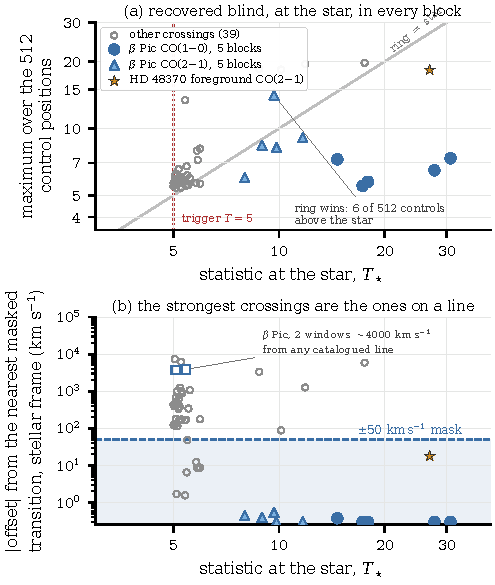
\includegraphics[width=0.88\columnwidth]{figures/bpic_control.pdf}
\caption{The $\beta$~Pictoris positive control, in both directions.
\emph{(a)}~The spatial screen. One point per execution block in which the
blind search recovers circumstellar carbon monoxide, plotted as the stellar
statistic against the maximum over that window's \NCtrl{} control positions:
the \NStageOneBpicEb{} blocks in which the star outranks every control, and
one further block in which the ring wins. \emph{The control is that the
search recovers a real narrow line at a stellar position, in two transitions
and in every one of these blocks.} It is not that the star outranks the ring
everywhere. In block \texttt{\BpCtrlBlock}, Band~\BpCtrlBand, the control
ring reaches \BpCtrlRingMax{} against \BpCtrlStar{} at the star, with
\BpCtrlNAbove{} of the \BpCtrlNCtrl{} control positions above it, so the
screen rejects a window holding carbon monoxide that is real, centred on the
star and independently mapped. The disc is resolved on the scale of the
primary beam in that configuration, which is the geometry the screen is
built to reject, so \textbf{the screen measures compactness and not
authenticity} (\S\ref{sec:bpicval}). \emph{(b)}~Line confusion, which is
what makes the screen's job hard. Each crossing is plotted by its velocity
offset from the nearest masked transition \emph{in its own star's rest
frame}, with the adopted $\pm\MaskHalfKms$\,km\,s$^{-1}$ half-width
marked. The \BpicPanelNCo{} $\beta$~Pictoris carbon-monoxide crossings land
\BpicDvCoLo--\BpicDvCoHi\,km\,s$^{-1}$ from CO, at the resolution of the
systemic velocity itself, while the two CS($5{\to}4$) crossings of the same
star sit \BpicDvCsLo--\BpicDvCsHi\,km\,s$^{-1}$ from anything catalogued
and are not attributed at any width. \BpicPanelNOther{} further crossings
are drawn in grey, with HD~48370 marked; \BpicPanelNDrawn{} of the
\NCross{} are plotted, the remainder being crossings for which the release
stores no control ring. \emph{A crossing is identified by where it falls in
this plane and not by how strong it is}, which is why the line mask and not
the trigger is the productive test.}
\label{fig:bpiccontrol}
\end{figure}
%
%% The line mask: the list, the frame, what it costs, and the three things a
%% reader has to be able to check -- the dates, the recurrence test applied to
%% the labelled crossings, and the image sideband.
%% Owner: r12-mask.  Carries \label{app:linemask} (cited by 04_method.tex and
%% app_C_spatialnorm.tex) and \label{tab:masklines}.
\section{The line mask}
\label{app:linemask}

A crossing that falls on a known molecular transition has an astrophysical
explanation to hand, and the mask exists to say which crossings those are. It
is a label and not a verdict: every crossing goes on to the spatial and
recurrence tests whether or not it carries the label, and the labelled
crossings are tested below.

\emph{The list, and when it was made.} The mask holds every transition of the
\FrNSpec{} species these spectral setups cover --- the three CO isotopologues,
HCN, HCO$^{+}$, CS, CN, SiO, H$_2$CO, SO, [C\,\textsc{i}] and hydrogen
recombination --- that falls inside one of the \McNIsland{} searched frequency
intervals with an upper-state energy below \McEuMax\,K. That rule is the whole
of it, and it admits \FrNTrans{} transitions
(Table~\ref{tab:masklines}). No strength cut is applied across species,
because the Einstein coefficients of the CO ladder are
$10^{-7}$--$10^{-6}$\,s$^{-1}$ and any threshold admitting the strong lines of
HCN would discard the brightest lines in these fields; within a species the
coefficient keeps a rotational transition with its main hyperfine components
and drops the weak satellites. The rarer isotopologues, $^{34}$SO and
H$^{13}$CN and the rest, are not among the named species and would add
\McNRare{} transitions. The list is a single Splatalogue query of CDMS and JPL
\citep{Pickett1998,CDMS2005} made on \MkListDate{} and frozen with the data
release, so it is reproducible as a file rather than as a description --- and
it therefore post-dates the \MkCritDate{} fixing of the disposition criteria,
as does every species in it. It is a uniform rule applied to all \NCross{}
crossings, not a record of what was recognised when each was first examined.

\emph{The frame is the star's own, and the sign is not the usual one.} A
crossing's frequency is carried from the topocentric value to the barycentre
using its own block's pointing and mid-time, and then to the stellar rest
frame using the star's systemic velocity. The barycentric term runs from
\FrBaryLo{} to \FrBaryHi\,km\,s$^{-1}$ across the survey, so a tolerance
applied in the observed frame would spend \FrBarySwing\,km\,s$^{-1}$ of its
budget on the Earth's motion. The \FrEpochNEpoch{} \FrEpochStar{} epochs show
the transform working in the only way that can be checked:
\FrEpochTopoKms\,km\,s$^{-1}$ apart as observed, they agree to
\FrEpochStelKms\,km\,s$^{-1}$ in the star's frame. Throughout,
$\Delta v_\star = c\,(\nu_\star-\nu_0)/\nu_0$, so a positive offset means the
crossing lies \emph{above} the transition in frequency --- the opposite sign
to the velocity convention of a spectral line.

\emph{The half-width, and what it costs.} A one-channel test is too tight for
circumstellar gas, whose emission is shifted by many channels: the tolerance
follows from Keplerian motion where these molecules survive,
$\lesssim$13\,km\,s$^{-1}$ beyond 10\,au, and is
$\pm\MaskHalfKms$\,km\,s$^{-1}$. At that width the mask removes
\FrMaskLostGHz\,GHz of the \FrMaskUnionGHz\,GHz unique-frequency union, which
is \FrMaskPct{} per cent of it; the loss is concentrated in the line-tuned
fine-channel windows, and the cost band by band is in the data release.
Between $\pm\FrLadderLo$ and $\pm\FrLadderHi$\,km\,s$^{-1}$ the mask labels
\FrAttrWTwenty{} to \FrAttrWHundred{} of the \NCross{} crossings, and the
\FrNRankPass{} unattributed crossing that outranks all \NCtrl{} control
positions in its own window is the same one at every width.

\begin{table}
\centering
\footnotesize
\caption{The line mask, by species: the number of transitions $N$ it holds,
the frequency range they span inside the searched intervals and their
upper-state energies. Hydrogen recombination lines carry no tabulated
$E_{\rm u}$. The transition-by-transition list is in the data release.}
\label{tab:masklines}
%% GENERATED by maskrecur_v413.py -- do not hand-edit.
\begin{tabular}{@{}lrr@{\,}c@{\,}rr@{}}
\hline
Species & $N$ & \multicolumn{3}{c}{$\nu_0$ (GHz)} & $E_{\rm u}$ (K) \\
\hline
H & 5 & 92.03 & -- & 231.90 & -- \\
SO & 15 & 100.03 & -- & 682.68 & 16--143 \\
H$_2$CO & 13 & 101.33 & -- & 491.97 & 10--106 \\
C$^{18}$O & 3 & 109.78 & -- & 329.33 & 5--32 \\
CN & 50 & 113.12 & -- & 680.30 & 5--114 \\
CO & 3 & 115.27 & -- & 345.80 & 6--33 \\
CS & 3 & 195.95 & -- & 342.88 & 24--66 \\
SiO & 2 & 217.10 & -- & 347.33 & 31--75 \\
$^{13}$CO & 8 & 220.40 & -- & 330.59 & 16--32 \\
HCN & 7 & 354.50 & -- & 354.51 & 43--43 \\
HCO$^{+}$ & 1 & 356.73 & -- & 356.73 & 43 \\
{[C\,\textsc{i}]} & 1 & 492.16 & -- & 492.16 & 24 \\
\hline
\end{tabular}%

\end{table}

\emph{Sulphur monoxide decides \MkNSODecideWord{} coincidences, and one rule is
applied to all of them.} \MkSOStars{} lie \MkSODvList\,km\,s$^{-1}$ from sulphur monoxide
transitions of upper-state energy \MkSOEuLo--\MkSOEuHi\,K, each inside a
Band~7 window that also covers CO($3\to2$), and none has a nearer transition
of any other masked species. There is reason for caution about each:
sulphur monoxide has not been reported in a debris disc, where the
second-generation gas is CO, C and O, and toward \FrCpStar{} the CO($3\to2$)
line is covered in the same window and absent to \FrCpCoLimMJy\,mJy in a
\FrCpCoChanKms\,km\,s$^{-1}$ channel. That caution applies equally to each of
them, and so does the date, since the species list post-dates every
classification; neither separates one coincidence from the others. Applying
the rule attributes all of them and gives \MkAttrSO{} attributed crossings
against \MkUnattrSO{} unattributed; withholding sulphur monoxide from all of
them instead gives \MkAttrNoSO{} and \MkUnattrNoSO, and returns a second
crossing to the \MkRankNoSO{} that outrank every control in their own
windows. The
recurrence test says the same thing about each of them either way, so the choice
moves counts and no conclusion.

\emph{The labelled crossings are tested for recurrence too.} Of the
\MkAttrSO{} attributed crossings, \MkAttrTested{} have a later execution block
covering the predicted cell. \MkAttrRecur{} are present again: toward
\MkAttrRecurStars{} a later block carries its own threshold crossing at the
same stellar-frame frequency, at $T_\star=\MkAttrRecurTLo$ to
\MkAttrRecurTHi, which is the test working in the positive direction on
emission that is certainly real. The other \MkAttrExcl{} are not present
again, and in each the repeat coverage is deep enough that a carrier at the
discovery flux would have exceeded the trigger there and does not; among them
are the sulphur monoxide coincidences, which the test limits to
\MkAttrExclLo--\MkAttrExclHi$\sigma$ whichever side of the mask they are
placed. \MkAttrUntest{} cannot be tested and are
named rather than counted: \MkAttrUntestNames, each observed once at the
frequency concerned.

\emph{Image-sideband leakage does not account for any crossing.} The mask
holds signal-sideband frequencies, so a bright line in the image sideband
could in principle be mistaken for a carrier. \MkImgN{} unattributed
crossings invite the question, at \MkImgFreqs\,GHz toward \MkImgStar, because
each shares a block with a CO($2\to1$) crossing at \MkImgPartner\,GHz in the
opposite sideband. A mirror about the first local oscillator would place that
line on the crossing only for an oscillator at
\MkImgLOReqLo--\MkImgLOReqHi\,GHz, and the block's own spectral windows
require \MkImgLOLo--\MkImgLOHi\,GHz: at the setting the mirror needs, the
lowest window of the block would sit at an intermediate frequency of
\MkImgIFReq\,GHz, beyond the \MkImgIFMax\,GHz the receiver provides
\citep{ALMAHandbook}. Their image frequencies fall at least
\MkImgDvMin\,km\,s$^{-1}$ from every masked transition.

\emph{A wider list is not a better one.} Every Splatalogue transition over the
searched intervals under the same energy cut and with an Einstein coefficient
above $10^{-5}$\,s$^{-1}$ --- \MaskDbTrans{} transitions of \MaskDbCarriers{}
species --- masks \MaskDbPctUnion{} per cent of the union and moves
\FrFullNFlip{} of the \NCross{} crossings across the line,
\FrFullNFlipRankWord{} of them a crossing that outranks every control, at
$\FrFullFlipRankDv$\,km\,s$^{-1}$ from a \FrFullFlipRankChem{} transition. At
these frequencies most frequencies lie within $\pm\MaskHalfKms$\,km\,s$^{-1}$
of something in such a list, which is why the species are restricted to what
these spectral setups cover, and why the outcome is a label. ``Coincident
with a known molecular line'' is a statement about a catalogue rather than a
property of a frequency.
%
%% APPENDIX D -- the false-alarm expectation, the control ensemble, and the
%% execution-block quality criterion.  Owner: r11-chain.  Carries
%% \label{app:falsealarm} (04_method.tex, 08_backmatter.tex) and
%% \label{sec:blockquality} (04_method.tex).
\section{The false-alarm expectation and the control ensemble}
\label{app:falsealarm}

The paper's central claim is that the number of unattributed crossings is the
number chance predicts. This appendix gives that expectation, what it is
conditioned on, and what the control ensemble calibrating it can support.

\subsection{What the expectation is conditioned on}
%% (subsection label retired: nothing cites it)

The expectation is built from the control positions themselves, which are the
only empirical null the data provide, and it imposes the condition an event
must actually satisfy: to reach the trigger, and to fall outside the
attribution windows. Each of the \NWinA{} Class~A windows of the census
contributes the fraction of its own \NCtrl{} control positions that reaches
the trigger, which is the probability that a position in that field does so
--- no cell count enters it and no form is assumed for the tail. Summed over
the windows, \StExpTrig{} are expected to trigger by chance; the attribution
windows occupy \LgMaskOccPct{} per cent of the searched band; and the product
is \textbf{\StExpChance{} expected unattributed Class~A crossings against
\StObs{} observed}, the two sides taken over the same windows and under the
same condition.

The one assumption that cannot be read off the searched data is that a star
behaves like a control position in its own field, and the reserved blocks
measure that in the quantity used here. Their stars reach the trigger in
\StHoObs{} of \StHoNFine{} fine-channel windows where the control positions
of those same windows predict \StHoExpFine: a ratio of \StHoRatio, with
\StHoLo--\StHoHi{} allowed by resampling the reserved blocks, and no two of
the events in one block. In the \StHoNCoarse{} coarse-channel reserved
windows no star reaches the trigger, against \StHoExpCoarse{} predicted. No
departure is detected and none is applied, and the limit is the one so few
events allow: a departure smaller than about \StHoAccPct{} per cent would not
have been seen, and that is the accuracy of every chance expectation in this
paper.

Every Class~B crossing in the survey comes from the one execution block of
\S\ref{sec:blockquality}. Setting that block aside, the
coarse class adds almost nothing to either side --- the expectation over both
classes together is \StExpSurv{} against the same \StObs{} observed --- so
the Class~A comparison is also the survey's. Only \NCtrlWinObs{} of the
\NWindows{} windows hold any control position above
$T_{\rm trig}=\StageNullTrig$ at all, and \StageNullEligibleA{} of those are
Class~A: a coarse single-pointing window has too few cells for its own field
to reach the trigger by chance.

\emph{One set of windows was extracted twice, and the second extraction is
the one adopted.} \StNRep{} windows were first extracted over a field that
excluded integrations lying inside the primary beam; re-extracting them
recovers a median \StRepOnsrc{} times the on-source time and shifts the
search statistic by a median \StRepDT, or \StRepDTAbs{} in absolute value.
The rule for which integrations a window keeps was fixed before any statistic
in this paper was computed, and the re-extracted value is adopted wherever it
exists: it carries \StRepAdopted{} rows of Table~\ref{tab:ledger} and takes
\StRepFell{} crossings below the trigger. A re-extracted window's control
ensemble is re-extracted with it, so neither side of the comparison above
mixes the two. The deposited catalogue holds the
first extraction's statistic and the shorter species list in its own columns,
so its disposition column and the adopted ledger disagree on those
\StRepFell{} crossings and on \StRepAttr{} more that the species list now
attributes. The ledger is the authority for every disposition quoted here.

\subsection{Execution-block quality}
\label{sec:blockquality}

The comparison with the control positions assumes each block's ensemble
behaves like noise, and one block makes that assumption plainly false: every
one of its \NCtrl{} probes exceeds the trigger, the smallest at
\BqFailCtrlMin. A criterion for the condition was therefore fixed and applied
to every block, rather than recognised on the block that prompted it.

The statistic is the one this paper already uses as a diagnostic: the median
of a window's control ensemble, which is what separates a field with a source
in it from a field that is no null at all. That median is a maximum over the
window's own channel$\times$drift grid, so its level rises with the cell
count; it is therefore scaled by the median of the same quantity over the
windows of its own search class, and one threshold then means the same thing
in both. A block's statistic is the median of that ratio over its windows,
and \textbf{a block fails when it exceeds \BqFactor{} the scale of its
class} --- the factor already carried by the window-level data-quality flag,
fixed before that flag was applied to anything.

Applied to all \BqNBlocks{} blocks of the primary census, where the median
block sits at \BqQMed, the criterion fails \BqNFail: \BqFailBlock{} toward
\BqFailStar, at \BqFailQ{} where the next worst block is \BqNextQ. Nothing
else is close, and the unscaled form of the rule fails the same
\BqRawNFail{} block. Its \BqFailNWin{} windows are all coarse-channel and
hold the survey's entire Class~B crossing population, so the block carries
\EvNCrossFlag{} of the \EvNCrossRaw{} raw threshold crossings and no Class~A
statistic in this paper has ever contained it. \textbf{The population the
paper characterises is therefore the \EvNCrossQp{} crossings in
quality-passing data}: \EvNAttrQp{} attributed, \EvNUnattrQp{} unattributed,
\EvNRankQp{} of those outranking all \NCtrl{} control positions of their own
window against \EvNRankFlag{} in the failed block. The other
\EvNCrossFlag{} appear in Table~\ref{tab:ledger}, with their block named, and
enter no count anywhere else.

\subsection{The control ensemble: its calibration, and its resolution}
%% (subsection label retired: nothing cites it)

The ring geometry is set in \S\ref{sec:statistic}; its calibration and its
resolution are the subject here. Under that geometry the stellar ranks are
consistent with the uniform distribution exchangeability implies, in both
array strata and over the \VerNTested{} windows that retain a control vector,
the ACA windows measured on the geometry of each observation's own antenna
table and baselines rather than on a 12\,m beam. The test is not a powerful
one: a shift of less than about \VerKsPowerAca{} in the rank distribution
could not have been seen in samples of this size, so the strata are
consistent with uniform rather than demonstrably uniform.

\emph{The rank is not a significance test, and the reason is structural.}
Ranking the star against \NCtrl{} control positions drawn from the same field
is a good way to decide which windows deserve examination, but
$1/(\NCtrl+1)=\RankFloorVal$ is the \emph{resolution} of the ensemble --- the
smallest rank it can express --- and not the probability that noise produced
the window. A survey of \NWindows{} windows needs
$0.05/\NWindows=\BonfScaleCalc$, so that floor is \BonfRankRatio{} times too
coarse, and correlation widens it: neighbouring controls are correlated below
the synthesised-beam scale, so a window's annulus carries only
$N_{\rm eff}\simeq30$--$43$ independent spatial trials and the ensemble
resolves no better than \RankEffLo--\RankEffHi. Drawing more controls does
not rescue it, the primary beam bounding how many independent positions a
single pointing contains. \textbf{That floor is the design's central
limitation: no single window in this survey can be significant on the rank
alone, which is why confirmation here requires independent recurrence.}

\subsection{The trials budget}

The searched cells counted in \S\ref{sec:summary} are not independent
trials: channel smoothing and a drift grid stepped twice per channel
correlate neighbouring ones, which alone would leave \StGridFrac{} of them
independent. The control ensembles say otherwise. Their maxima sit at
\CtrlMaxRatioMed{} of the prediction for the maximum of the full searched
count treated as independent and Gaussian, a budget that predicts
\NCtrlWinExp{} windows carrying a control above $T_{\rm trig}$ against the
\NCtrlWinObs{} observed; and fitting each window's effective count against
its own ensemble returns \StNindFrac{} of its searched cells. Nothing quoted
here turns on which figure is right, because the expectation above is summed
from the measured exceedance rates and not from a cell count; by the
cell-count route it is \StExpModel, \StModelAgreePct{} per cent away.

\emph{The on-star crossings do exceed that budget, and the attribution
accounts for it.} A Gaussian tail over every cell the survey searched
predicts \CellExpect{} stellar exceedances against the \NCross{} found, but
\NAttributed{} of those are identified with a catalogued transition and
\EvNCrossFlag{} come from the block of \S\ref{sec:blockquality}; what is left
is the \StObs{} unattributed crossings in quality-passing data against
\StExpSurv{} predicted. No excess of chance crossings survives the
attribution, which is the comparison the paper rests on.

\emph{One stratum departs from uniformity and it is the one that matters.}
The quantity is the number of windows whose stellar peak both reaches the
trigger and exceeds all \NCtrl{} of that window's own control positions, and
over $n=\NFine$ fine-channel windows it is not uniform: \NStageOneFine{}
such windows against \ExpStageOneFine{} expected, while the coarse stratum,
three times larger and predicting \ExpStageOneCoarse, contains
\NStageOneCoarse{} --- including none of the \EvNCrossFlag{} crossings of the
flagged block, whose statistics stand below their own re-extracted control
maxima. A coarse channel dilutes a narrow circumstellar line, so
the class that can resolve one is the class that finds it --- and by the same
reasoning a genuine unresolved carrier would appear in Class~A first. The
departure survives removal of every fine window carrying a stellar crossing,
so fine-window rank probabilities are optimistic for the class as a whole and
not only where a crossing sits.

\emph{What is left is bounded, and the bounds are null.} Treating each
control as a pseudo-star and ranking it against the other \NCtrl-1 gives
\NPseudo{} ranks that the real stellar ranks agree with at
$\pv{\StarPseudoP}$; any systematic radial suppression of the controls is
below \RingRhoBoundPct{} per cent in the mean; and scrambling each window so
that nothing coherent survives along a drift track carries \LNNWindows{}
windows past the rank floor and changes no disposition.

%% ------------------------------------------------------------------
%% The chance expectation in this appendix is summed from the measured
%% control exceedance rates (stats_v413.py, round 260), so no cell count
%% and no Gaussian tail enters it; the cell-count route is quoted beside
%% it as a cross-check.  The rank-conditioned expectation
%% (\ClustStageMean against \ClustStageNObs) is a pipeline diagnostic and
%% must not be reachable as "the" expectation.
%% Floats held in the data release rather than here: tab:ctrlsep,
%% tab:excess, tab:arraysplit, fig:ctrldiag.  None is cited from the body.
%% ------------------------------------------------------------------

%% ★ tab:ledger MOVED HERE from Sec. 5 in the v4.12 length pass: the
%% crossing-by-crossing ledger belongs beside the false-alarm accounting that
%% explains how many of its rows are expected.  0.72 pp off the main text.
\begin{table*}
\centering
\caption{\textbf{The crossing ledger, from which every disposition in this
paper can be reproduced.} All \EvNCrossRaw{} threshold crossings, the
\EvNCrossFlag{} in the flagged block of \S\ref{sec:bdblock} among them and
labelled as such: the star, its execution block, the ALMA band, the crossing
frequency as the correlator delivered it and the same frequency in the star's
rest frame, the search statistic $T_\star$, the largest statistic
$T_{\rm ctrl}$ among the window's \NCtrl{} control positions, the nearest
masked transition and the stellar-frame offset $\Delta v_\star$ from it, then
the recurrence test: $n_{\rm rep}$ covering repeat blocks spanning $\Delta t$
days, the statistic $T_{\rm pers}$ a carrier persisting at the discovery flux
would have produced at the predicted stellar-frame cell, the statistic
$T_{\rm rep}$ measured there at the carried drift, combining the repeat
epochs by inverse variance, and the exclusion
$\sigma_{\rm excl}=(T_{\rm pers}-T_{\rm rep})/\sqrt{1+(T_{\rm pers}/T_\star)^2}$
(Eq.~\ref{eq:excl}), which is therefore reproducible from three columns of
this table. The fraction of the discovery amplitude still ruled out at the
trigger, $(T_{\rm rep}+5)/T_{\rm pers}$, follows from two of them.
$T_\star$ and $T_{\rm ctrl}$ always come from the same extraction of the same
window, so the comparison between them is one a reader can make;
$T_{\rm ctrl}$ gates nothing and says only which crossing was examined
first, and the drift-maximised reading of the cell is in
Table~\ref{tab:cand} for the two leading events and in the data release for
the rest. On the flagged rows $T_{\rm pers}$ and the exclusion, which would
inherit a discovery amplitude from the failing block, are withheld. A
crossing is attributed where
$|\Delta v_\star|\le\MaskHalfKms$\,km\,s$^{-1}$ and the transition named is
the nearest in that frame, so far from every transition it is the magnitude
and not the name that carries information. Block identifiers omit the
constant \texttt{A002\_} prefix.}
\label{tab:ledger}
\tiny
%% GENERATED by ledger_v410.py -- do not hand-edit.
%% One row per threshold crossing, one epoch convention, stellar-frame attribution.
%% part 1 of 2, 28 rows; the split is made in the generator so the float cannot outgrow its page.
\begin{tabular}{@{}l@{\hspace{0.9pt}}l@{\hspace{0.9pt}}c@{\hspace{0.9pt}}r@{\hspace{0.9pt}}r@{\hspace{0.9pt}}r@{\hspace{0.9pt}}r@{\hspace{0.9pt}}l@{\hspace{0.9pt}}r@{\hspace{0.9pt}}r@{\hspace{0.9pt}}r@{\hspace{0.9pt}}r@{\hspace{0.9pt}}r@{\hspace{0.9pt}}r@{\hspace{0.9pt}}l@{}}
\hline
Star & block & B & $\nu_{\rm topo}$ (GHz) & $\nu_{\star}$ (GHz) & $T_\star$ & $T_{\rm ctrl}$ & line & $\Delta v_{\star}$ & $n_{\rm rep}$ & $\Delta t$ (d) & $T_{\rm pers}$ & $T_{\rm rep}$ & $\sigma_{\rm excl}$ & disposition \\
\hline
BD+05 1668 & Xc7fa6f\_X28a8 & 6 & 240.1016 & 240.1054 & 73.398 & 74.69 & CS($5$--$4$) & -5911.9 & 29 & 0.9--113 & n/a & +0.15 & n/a & unattributed; flagged \\
BD+05 1668 & Xc7fa6f\_X28a8 & 6 & 224.7422 & 224.7458 & 48.303 & 83.74 & H$_2$CO($3_{1,2}$--$2_{1,1}$) & -1264.5 & 29 & 0.9--113 & n/a & +0.37 & n/a & unattributed; flagged \\
BD+05 1668 & Xc7fa6f\_X28a8 & 6 & 226.7422 & 226.7458 & 41.355 & 75.48 & CN($2_{3/2}$--$1_{1/2}$) & +88.0 & 29 & 0.9--113 & n/a & +0.66 & n/a & unattributed; flagged \\
BD+05 1668 & Xc7fa6f\_X28a8 & 6 & 242.1953 & 242.1992 & 39.586 & 83.29 & CS($5$--$4$) & -3349.2 & 29 & 0.9--113 & n/a & +0.77 & n/a & unattributed; flagged \\
$\beta$~Pic & Xf5d76d\_Xeb8 & 3 & 115.2603 & 115.2711 & 30.765 & 7.34 & CO($1$--$0$) & -0.2 & --- & --- & --- & --- & --- & attributed \\
$\beta$~Pic & Xf5d76d\_Xe19 & 3 & 115.2603 & 115.2711 & 27.684 & 6.48 & CO($1$--$0$) & -0.2 & --- & --- & --- & --- & --- & attributed \\
HD 48370 & Xc26103\_X155a & 6 & 230.5117 & 230.5243 & 26.834 & 18.36 & CO($2$--$1$) & -17.8 & --- & --- & n/a & --- & n/a & attributed; flagged \\
$\beta$~Pic & Xf4df6f\_Xc7 & 3 & 115.2620 & 115.2711 & 17.907 & 5.76 & CO($1$--$0$) & -0.2 & --- & --- & --- & --- & --- & attributed \\
$\beta$~Pic & Xf5d76d\_Xcc5 & 3 & 115.2604 & 115.2711 & 17.288 & 5.52 & CO($1$--$0$) & -0.2 & --- & --- & --- & --- & --- & attributed \\
$\beta$~Pic & Xf5d76d\_X32f1 & 3 & 115.2606 & 115.2713 & 14.654 & 7.27 & CO($1$--$0$) & +0.4 & --- & --- & --- & --- & --- & attributed \\
$\beta$~Pic & Xd9668b\_X3a90 & 6 & 230.5161 & 230.5378 & 11.681 & 9.12 & CO($2$--$1$) & -0.3 & --- & --- & --- & --- & --- & attributed \\
$\beta$~Pic & X6f1341\_X1484 & 6 & 230.5284 & 230.5379 & 9.832 & 8.20 & CO($2$--$1$) & -0.1 & --- & --- & --- & --- & --- & attributed \\
$\beta$~Pic & X7116f1\_X1785 & 6 & 230.5272 & 230.5384 & 9.677 & 14.13 & CO($2$--$1$) & +0.5 & --- & --- & --- & --- & --- & attributed \\
$\beta$~Pic & Xd9668b\_Xa9df & 6 & 230.5160 & 230.5377 & 8.948 & 8.41 & CO($2$--$1$) & -0.4 & --- & --- & --- & --- & --- & attributed \\
$\beta$~Pic & Xa7a216\_X23e4 & 6 & 230.5273 & 230.5377 & 7.988 & 6.03 & CO($2$--$1$) & -0.4 & --- & --- & --- & --- & --- & attributed \\
61 Vir & Xc079b5\_X82f & 7 & 346.3138 & 346.3232 & 5.958 & 5.65 & SO($9_{8}$--$8_{7}$) & -177.6 & 3 & 0.1--3.0 & 9.7 & +0.39 & 4.9 & unattributed; no recurrence \\
HD 285968 & Xd98580\_X3bf6 & 6 & 230.5021 & 230.5447 & 5.956 & 8.12 & CO($2$--$1$) & +8.7 & --- & --- & --- & --- & --- & attributed \\
HD 285968 & Xdb7ab7\_X5b4e & 6 & 230.5116 & 230.5447 & 5.868 & 7.22 & CO($2$--$1$) & +8.7 & --- & --- & --- & --- & --- & attributed \\
HD 285968 & Xdb4b9a\_X108f & 6 & 230.5100 & 230.5447 & 5.835 & 7.94 & CO($2$--$1$) & +8.7 & --- & --- & --- & --- & --- & attributed \\
CP$-$72 2713 & Xff0235\_X4a6d & 7 & 344.2697 & 344.2965 & 5.809 & 5.68 & SO($8_{8}$--$7_{7}$) & -12.3 & 5 & 0.1--2.1 & 6.3 & -0.82 & 4.8 & attributed \\
HD~139084~B & Xcd8029\_Xb6b0 & 7 & 345.8241 & 345.8241 & 5.763 & 17.70 & CO($3$--$2$) & +24.4 & --- & --- & --- & --- & --- & attributed \\
HD 14055 & Xfff3d8\_Xd46 & 7 & 331.7699 & 331.7664 & 5.575 & 5.99 & $^{13}$CO($3$--$2$) & +1068.7 & 30 & 0.9--650 & 170.4 & -0.02 & 5.6 & unattributed; no recurrence \\
HD 23484 & X10b22d7\_X2445 & 6 & 230.7904 & 230.8006 & 5.520 & 5.55 & CO($2$--$1$) & +341.5 & 4 & 0.1--2.1 & 10.4 & +1.25 & 4.3 & unattributed; no recurrence \\
HD 161868 & Xff45a6\_X10ca8 & 7 & 345.6338 & 345.6491 & 5.481 & 6.16 & SO($2_{3}$--$2_{1}$) & -48.0 & 13 & 0.0--6.1 & 92.2 & +0.24 & 5.5 & attributed \\
HIP 10679 & Xa95c04\_X14cd & 6 & 220.4185 & 220.4035 & 5.456 & 6.76 & $^{13}$CO($2$--$1$) & +6.5 & --- & --- & --- & --- & --- & attributed \\
HD~14055 & X11adad7\_X25c5e & 7 & 345.4564 & 345.4303 & 5.448 & 6.82 & SO($2_{3}$--$2_{1}$) & -237.8 & 30 & 0.1--653 & 14.0 & +0.03 & 5.1 & unattributed; no recurrence \\
HD 207129 & Xc19d6f\_X5706 & 6 & 230.4226 & 230.4070 & 5.433 & 5.52 & CO($2$--$1$) & -170.3 & 4 & 0.8--425 & 69.7 & -0.93 & 5.5 & unattributed; no recurrence \\
$\beta$~Pic & Xd9668b\_X3a90 & 6 & 241.7512 & 241.7739 & 5.420 & 5.81 & CS($5$--$4$) & -3869.7 & 1 & 1.0 & 5.7 & +0.72 & 3.4 & unattributed; no recurrence \\
\hline
\end{tabular}

\end{table*}

%% ★ GLENN, 2026-10-06: the bottom of this table ran into the text beneath
%% it.  A `table*` cannot break across pages and the ledger is a row per
%% threshold crossing, so the cure is structural and lives in the generator:
%% `ledger_v410.py` writes the body in parts of at most 28 rows and asserts
%% that it has enough floats for them.  This is the continuation; its caption
%% is one line, because the first carries the definitions.
\begin{table*}
\centering
\caption{\emph{The crossing ledger, continued.} The remaining
\CxLedgerPartTwo{} of the \EvNCrossRaw{} threshold crossings, in the same
order and with the same columns as Table~\ref{tab:ledger}, whose caption
defines them.}
\label{tab:ledgercont}
\tiny
%% GENERATED by ledger_v410.py -- do not hand-edit.
%% One row per threshold crossing, one epoch convention, stellar-frame attribution.
%% part 2 of 2, 28 rows; the split is made in the generator so the float cannot outgrow its page.
\begin{tabular}{@{}l@{\hspace{0.9pt}}l@{\hspace{0.9pt}}c@{\hspace{0.9pt}}r@{\hspace{0.9pt}}r@{\hspace{0.9pt}}r@{\hspace{0.9pt}}r@{\hspace{0.9pt}}l@{\hspace{0.9pt}}r@{\hspace{0.9pt}}r@{\hspace{0.9pt}}r@{\hspace{0.9pt}}r@{\hspace{0.9pt}}r@{\hspace{0.9pt}}r@{\hspace{0.9pt}}l@{}}
\hline
Star & block & B & $\nu_{\rm topo}$ (GHz) & $\nu_{\star}$ (GHz) & $T_\star$ & $T_{\rm ctrl}$ & line & $\Delta v_{\star}$ & $n_{\rm rep}$ & $\Delta t$ (d) & $T_{\rm pers}$ & $T_{\rm rep}$ & $\sigma_{\rm excl}$ & disposition \\
\hline
HR~1010 & Xc6fa08\_X1053 & 6 & 230.5133 & 230.5287 & 5.410 & 5.65 & CO($2$--$1$) & -12.0 & --- & --- & --- & --- & --- & attributed \\
ALMA J153702653-33192492 & Xff0235\_X8392 & 6 & 230.5222 & 230.5392 & 5.405 & 13.41 & CO($2$--$1$) & +1.6 & --- & --- & --- & --- & --- & attributed \\
HD 110411 & Xe45e29\_Xb7d4 & 6 & 219.4538 & 219.4357 & 5.393 & 5.85 & C$^{18}$O($2$--$1$) & -170.2 & 1 & 10 & 6.7 & +0.62 & 3.8 & unattributed; no recurrence \\
HD 31392 & X129754b\_X6946 & 6 & 231.1998 & 231.2231 & 5.289 & 5.81 & H($30\alpha$) & -876.3 & 8 & 0.1--41 & 15.7 & -0.26 & 5.1 & unattributed; no recurrence \\
HD 14055 & Xff99e1\_X24be0 & 7 & 331.7078 & 331.7035 & 5.277 & 5.69 & $^{13}$CO($3$--$2$) & +1011.6 & 30 & 0.9--652 & 252.2 & +0.15 & 5.3 & unattributed; no recurrence \\
AU Mic & Xa42f75\_X319 & 6 & 230.6864 & 230.6705 & 5.274 & 6.07 & CO($2$--$1$) & +172.3 & 2 & 310--455 & 6.4 & -0.16 & 4.2 & unattributed; no recurrence \\
HD 69830 & X12209f7\_X16edb & 7 & 322.4325 & 322.4444 & 5.259 & 5.42 & C$^{18}$O($3$--$2$) & -6268.5 & 5 & 0.1--29 & 8.9 & -0.48 & 4.8 & unattributed; no recurrence \\
ALMA J153702653-33192492 & Xfe62c1\_X398 & 6 & 216.1844 & 216.2036 & 5.228 & 6.02 & SiO($5$--$4$) & -1244.6 & 7 & 18--126 & 11.0 & +1.03 & 4.3 & unattributed; no recurrence \\
AU Mic & X899169\_X1838 & 6 & 230.8252 & 230.8294 & 5.221 & 5.85 & CO($2$--$1$) & +379.0 & 2 & 145--310 & 10.0 & +0.19 & 4.5 & unattributed; no recurrence \\
HD 14055 & Xff99e1\_X2c3bb & 7 & 345.5256 & 345.5216 & 5.186 & 5.66 & SO($2_{3}$--$2_{1}$) & -158.6 & 30 & 0.1--651 & 172.8 & +2.00 & 5.1 & unattributed; no recurrence \\
HD 14055 & Xfffde1\_X3835 & 7 & 345.0099 & 345.0070 & 5.177 & 6.56 & SO($2_{3}$--$2_{1}$) & -604.8 & 30 & 0.1--649 & 187.2 & -1.78 & 5.2 & unattributed; no recurrence \\
HD 14055 & Xff99e1\_X2b2ee & 7 & 344.7007 & 344.6965 & 5.175 & 5.92 & SO($8_{8}$--$7_{7}$) & +336.0 & 30 & 0.1--651 & 210.7 & -0.00 & 5.2 & unattributed; no recurrence \\
LHS 1140 & Xd9d7c7\_X6fd2 & 6 & 230.6355 & 230.6268 & 5.136 & 5.68 & CO($2$--$1$) & +115.5 & 4 & 5.0--27 & 7.3 & +0.33 & 4.0 & unattributed; no recurrence \\
HD 10647 & Xff294f\_Xaf70 & 7 & 331.6570 & 331.6943 & 5.120 & 5.91 & $^{13}$CO($3$--$2$) & +1003.3 & 10 & 0.1--592 & 125.8 & +0.39 & 5.1 & unattributed; no recurrence \\
CD$-$57 1054 & Xcf525f\_X5aa4 & 7 & 346.5099 & 346.5265 & 5.108 & 5.71 & SO($9_{8}$--$8_{7}$) & -1.7 & 1 & 39 & 6.0 & -0.27 & 4.1 & attributed \\
ALMA J153702653-33192492 & Xf8f6a9\_X10359 & 6 & 217.7292 & 217.7269 & 5.091 & 5.41 & H$_2$CO($3_{0,3}$--$2_{0,2}$) & -680.5 & 7 & 3.8--242 & 11.6 & +0.07 & 4.6 & unattributed; no recurrence \\
GJ 849 & Xd9668b\_X841a & 6 & 230.8769 & 230.8581 & 5.090 & 5.83 & CO($2$--$1$) & +416.3 & 5 & 0.1--51 & 9.3 & -1.69 & 5.3 & unattributed; no recurrence \\
ALMA J153702653-33192492 & Xfe62c1\_X398 & 6 & 218.8729 & 218.8923 & 5.090 & 5.56 & H$_2$CO($3_{2,1}$--$2_{2,0}$) & +181.2 & 7 & 18--126 & 10.5 & -1.04 & 5.0 & unattributed; no recurrence \\
HD 14055 & X1001fdc\_X29ae & 7 & 331.1559 & 331.1546 & 5.082 & 6.26 & $^{13}$CO($3$--$2$) & +513.8 & --- & --- & --- & --- & --- & unattributed; no spectrum \\
$\beta$~Pic & Xd9668b\_Xa9df & 6 & 241.8367 & 241.8594 & 5.079 & 5.99 & CS($5$--$4$) & -3765.1 & 1 & 1.0 & 4.8 & -0.63 & 3.9 & unattributed; no recurrence \\
ALMA J153702653-33192492 & Xf8f6a9\_X10359 & 6 & 218.6711 & 218.6688 & 5.048 & 5.77 & H$_2$CO($3_{2,1}$--$2_{2,0}$) & -125.1 & 7 & 3.8--242 & 11.6 & +0.00 & 4.6 & unattributed; no recurrence \\
HD 69830 & X12277ed\_X178c6 & 7 & 321.2005 & 321.2149 & 5.046 & 6.13 & C$^{18}$O($3$--$2$) & -7387.7 & 5 & 6.0--36 & 10.2 & -0.46 & 4.7 & unattributed; no recurrence \\
HR 1010 & Xc66ce1\_Xaa9 & 6 & 230.8348 & 230.8491 & 5.044 & 5.72 & CO($2$--$1$) & +404.6 & 7 & 1.1--14 & 10.3 & -1.53 & 5.2 & unattributed; no recurrence \\
61 Vir & Xc067f7\_X822 & 7 & 345.5599 & 345.5678 & 5.038 & 5.79 & SO($2_{3}$--$2_{1}$) & -118.5 & 3 & 2.0--3.0 & 9.3 & +0.45 & 4.2 & unattributed; no recurrence \\
HD 170773 & Xff0235\_X8c42 & 7 & 331.0101 & 331.0234 & 5.029 & 5.75 & $^{13}$CO($3$--$2$) & +394.8 & 4 & 0.9--113 & 74.8 & +1.56 & 4.9 & unattributed; no recurrence \\
ALMA J153702653-33192492 & Xd9d7c7\_Xbb64 & 7 & 347.2179 & 347.1890 & 5.009 & 5.68 & SiO($8$--$7$) & -122.2 & 1 & 0.1 & 5.0 & -2.06 & 5.0 & unattributed; no recurrence \\
HD~14055 & X1190de8\_Xd526 & 7 & 344.4676 & 344.4515 & 5.006 & 5.96 & SO($8_{8}$--$7_{7}$) & +122.7 & 30 & 20--611 & 11.6 & -0.60 & 4.8 & unattributed; no recurrence \\
$\eta$~Crv & X122b6ff\_X1041e & 7 & 357.2815 & 357.2475 & 5.006 & 5.50 & HCO$^{+}$($4$--$3$) & +431.3 & 1 & 87 & 11.0 & -0.62 & 4.8 & unattributed; no recurrence \\
\hline
\end{tabular}

\end{table*}
%
%% APPENDIX E -- radio-frequency interference screening.
%% Owner: appendix-triage.  Carries \label{app:rfi}.
\section{Radio-frequency interference screening}
\label{app:rfi}

Interference is the first alternative explanation for an unattributed
crossing, so the screening this survey has, and the coverage it does not
have, are both set out here. Millimetre interferometry is an unusually poor
environment for terrestrial interference, though not an empty one: ITU Radio
Regulations Article~5 \citep{ITU2024} carries active allocations throughout
90--275\,GHz and WRC-19 identified parts of 275--450\,GHz for land-mobile and
fixed use. The specific hazard is the \RadarLo--\RadarHi\,GHz Earth
exploration-satellite allocation used by spaceborne cloud radar
\citep{CloudSat2002,EarthCARE2023}, a documented contaminant of ALMA Band~3;
\RadarNWin{} of the \RadarNTot{} searched windows overlaps it, carrying
\RadarNCross{} threshold crossings and \RadarNStage{} rank-passing events, so
no result here rests on it. What favours this band is that terrestrial
transmitters are sparse compared with centimetre wavelengths, that the array
sits at 5000\,m on a site chosen partly for radio quietness, and, decisively,
that an interferometer is not a total-power detector: a signal not in the far
field at the phase centre does not fringe-track but acquires a rapidly
varying geometric phase across the array, and is suppressed in the
correlation rather than imaged.

\emph{The coverage of the screening is uneven, and that is stated rather than
smoothed over.} The allocation test above and the sky- and
intermediate-frequency tests below are computed for every searched window
from the released catalogue, as is the \NCtrl-position rank screen, which
asks whether an excess is at the star or everywhere in the field. Recurrence
reaches only the crossings with a covering repeat block, and the visibility
fit is a consistency check rather than a filter. The correlator flagging is
the observatory's own, replayed from each block's delivered calibration
script, but it is not recorded per window in the release. \emph{No
per-channel interference flag of our own exists, and none can be recovered.}
Three measurements follow, and each is a test the population could have
failed.

\emph{First, clustering in sky frequency.} If interference dominated the
crossing population, the crossings would pile up at particular sky
frequencies. They do cluster --- but on the survey's own molecular lines.
The test needs a measured peak frequency in the frame in which an interfering
carrier would stand still, so it runs topocentrically over the
\AppMNCrossF{} of the \EvNCrossRaw{} crossings for which the release records
one, against the transitions the search was tuned to. For the other
\CsNCrossNoFreq, all \CsCrossNoFreqStar{} carbon-monoxide crossings, the
release gives the velocity offset from the line instead, and a frequency
reconstructed from a line offset cannot be used to ask whether frequencies
crowd onto lines. Of the \AppMNCrossF, \AppMTubeObs{} fall within
$\pm\DispoHalfKms$\,km\,s$^{-1}$ of a searched transition against
\AppMTubeNull{} expected if each window's peak fell anywhere on that
window's own channel grid, $\pv{\AppMTubeP}$. The densest band,
\AppMBandLo--\AppMBandHi\,GHz, holds \AppMBandN{} of them, \AppMBandNAttr{}
within that velocity window of CO($2{\to}1$); and once the line-attributed
crossings are set aside, the \AppMUnattrN{} that remain show no clustering at
all ($\pv{\AppMUnattrP}$). \emph{The concentration is the attribution, not a
residue left over after it.} Table~\ref{tab:ledger} counts the same band as
\EvTubeLedgerN{} crossings with \EvTubeLedgerAttr{} attributed, because it is
a different test over a different set --- all \EvNCrossRaw, each attributed
in its own star's rest frame --- and the \EvTubeExtra{} it adds are exactly
the ones whose peak frequency this test has no measurement of.

\emph{Second, fixed intermediate frequency.} An artefact of the signal chain
would sit at a fixed position within the spectral window rather than at a
fixed sky frequency. This test is run over every window for which the
catalogue releases a peak frequency --- \IfPopNWin{} of the \NWindows{}, of
which only \IfPopNCross{} carry a threshold crossing --- because such an artefact would
occupy the same intermediate frequency in all of them and not only where the
trigger fires. It does not: the peaks' fractional positions within their own
windows have median \RfiFracMed{} and are uniform.

\emph{Third, a cross-target occupancy screen over every searched window and
not only the crossings.} Interference belongs to the observatory and not to
the star, so a terrestrial carrier should recur at the same sky frequency
toward \emph{unrelated} stars. It does not even for the leading event:
\RfiEventLead; \RfiOtherWin{} further windows, toward \RfiOtherStarsRange{}
other stars in \RfiOtherBlocksRange{} other blocks, cover \RfiFreqThem, and
\RfiSameChanClause.\RfiNotTestableClause{} Over all \RfiOccNWin{} searched
windows toward \RfiOccNStars{} stars, with each window's peak randomised on
its own channel grid, the number of cross-star coincidences within
\RfiOccTol\,MHz is \RfiOccObs{} against
\RfiOccNull$\,\pm\,$\RfiOccNullSd{} expected ($\pv{\RfiOccP}$); among the
\RfiOccSigN{} windows whose peak exceeds the trigger it is \RfiOccSigObs{}
against \RfiOccSigNull$\,\pm\,$\RfiOccSigNullSd, i.e.\ \emph{below} the
null, and with the molecular-line mask applied \RfiOccMskObs{} against
\RfiOccMskNull$\,\pm\,$\RfiOccMskNullSd. There is no excess to explain. Two
features of the screen matter. It is keyed on the star and not on the product
directory, because a star's own repeat observations are not different
targets; and \RfiOccMaskN{} of those \RfiOccSigN{} windows sit on a masked
transition (\RfiOccSpeciesList), so the mask has to be applied first --- a
carbon monoxide line falls at nearly the same sky frequency toward every
nearby star, which is exactly the coincidence the screen is looking for.

\emph{One execution block fails these tests, and it fails them as a block
rather than as a carrier.} Its \DqBlockNCross{} crossings toward
\LgVerRejectStar{} are the highest statistics in the survey outside
$\beta$~Pictoris and HD~48370, and the field statistics that identify the
failure are in \S\ref{sec:bdblock}. What belongs here is whether
interference accounts for it, and three readings say not. The visibility fit
returns a large imaginary part, placing the emission away from the phase
centre. The block's \BdNSibling{} sibling executions of the same field, with
the same array and the same spectral setup, produce no crossing at all. And
it is not a carrier at a fixed sky frequency: each of the four frequencies is
covered by \DqOtherWinLo--\DqOtherWinHi{} further windows toward
\DqOtherStarLo--\DqOtherStarHi{} other stars, and \DqOtherSame{} of them
carries a crossing in the same channel.

\emph{One reading does point at a mechanism, and it can be tested across the
survey.} \DqBlockIfMult{} of the \DqBlockNCross{} sit at the identical
channel of two different spectral windows, which is the signature of a fixed
intermediate frequency --- and a feature with no geometric fringe phase, a
spur common to every antenna being the obvious case, does not fringe-track,
so it gathers at the phase centre rather than at the star. Here the two are a
twentieth of an arcsecond apart, so the block cannot test its own hypothesis;
the survey can, because the star lies \EvPcOffLo--\EvPcOffHi\,arcsec from the
phase centre in \EvPcNWin{} windows whose control annulus brackets it,
putting a median of \EvPcNNear{} probes within two synthesised beams of the
phase centre and the star well outside. Against the probes at the same
distance from the star but elsewhere in azimuth --- matching the radius
matters, or a centrally concentrated disc would imitate the effect --- those
probes are higher by $\EvPcDiff\pm\EvPcErr$ in the statistic, consistent with
zero and bounded by \EvPcBound, smaller by a factor of about \EvPcFactor{}
than the \EvPcNeed{} by which this block's ring is raised. \emph{The phase
centre is not where the excess lives.}
\textbf{The evidence supports a
data-quality failure of one execution block, and that is how these
\EvNCrossFlag{} crossings are dispositioned} (\S\ref{sec:bdblock}): the
criterion of Appendix~\ref{sec:blockquality} flags \DqNWin{} of the
\NWindows{} windows, toward \DqNStar{} stars (\DqStars), the second being a
resolved disc rather than a defect.

\emph{None of this is a substitute for the ON/OFF cadence a dedicated search
uses, and we do not present it as one.} We claim only that \emph{no
identified interference mechanism accounts for the unattributed events}:
allocation tables cannot exclude harmonics, intermodulation products,
unconventional emitters or near-field sources, and archival data without a
simultaneous off-source strategy cannot do better. The three tests establish
that the crossing population as a whole carries none of the signatures
interference leaves, which is a statement about the population and not a
clearance of any individual crossing.

%% ------------------------------------------------------------------
%% NOTE: per 06_discussion.tex's own R6, this appendix no longer ends on
%% "the null result resting on internal validation alone" -- that statement
%% now lives once, in the discussion's lessons subsection.
%% REQUEST (appendix-triage -> integrator):
%%   fig:appm (the power comparison of the per-channel multiplicity statistic
%%   against the scan statistic) is deleted: it exists to compare our own two
%%   statistics, and the paper now states only the one it uses.  The
%%   \AppMPowerOld* and \RfiOcc{Prior,Dir,Stale}* macro families are no
%%   longer referenced and will be retired.  figures/appm_power.pdf is no
%%   longer included.
%% ------------------------------------------------------------------
%
\begin{thebibliography}{99}
\bibitem[Astropy Collaboration et al.(2022)]{Astropy2022} Astropy Collab., 2022, ApJ, 935, 167
\bibitem[Backus \& Project Phoenix Team(2002)]{Backus2002} Backus P.~R., Project Phoenix Team, 2002, in Stanimirovi\'{c} S., Altschuler D., Goldsmith P., Salter C., eds, ASP Conf. Ser. Vol. 278, Single-Dish Radio Astronomy: Techniques and Applications. Astron. Soc. Pac., San Francisco, p.~525
\bibitem[Akeson et al.(2013)]{NEA2013} Akeson R.~L., et al., 2013, PASP, 125, 989
\bibitem[Cortes et al.(2024)]{ALMAHandbook} Cortes P.~C., et al., 2024, ALMA Technical Handbook, ALMA Doc. 11.3, ver. 1.4
\bibitem[International Telecommunication Union(2024)]{ITU2024} International Telecommunication Union, 2024, Radio Regulations, Edition of 2024. ITU, Geneva
\bibitem[Remijan et al.(2007)]{Splatalogue2007} Remijan A.~J., Markwick-Kemper A., ALMA Working Group on Spectral Line Frequencies, 2007, in American Astronomical Society Meeting Abstracts 211, 132.11
\bibitem[Stephens et al.(2002)]{CloudSat2002} Stephens G.~L., et al., 2002, Bull. Am. Meteorol. Soc., 83, 1771
\bibitem[Wehr et al.(2023)]{EarthCARE2023} Wehr T., et al., 2023, Atmos. Meas. Tech., 16, 3581
\bibitem[CASA Team et al.(2022)]{CASA2022} CASA Team, 2022, PASP, 134, 114501
\bibitem[Burton et al.(2022)]{Burton2022} Burton K., MacGregor M. A., Osten R. A., 2022, ApJL, 939, L6
\bibitem[Cataldi et al.(2023)]{Cataldi2023} Cataldi G., et al., 2023, ApJ, 951, 111
\bibitem[Choza et al.(2024)]{Choza2024} Choza C., et al., 2024, AJ, 167, 10
\bibitem[Cocconi \& Morrison(1959)]{CocconiMorrison1959} Cocconi G., Morrison P., 1959, Nature, 184, 844
\bibitem[Czech et al.(2021)]{Czech2021} Czech D.~J., et al., 2021, PASP, 133, 064502
\bibitem[Dent et al.(2014)]{Dent2014} Dent W. R. F., et al., 2014, Science, 343, 1490
\bibitem[Drake(1961)]{Drake1960} Drake F.~D., 1961, Physics Today, 14(4), 40
\bibitem[Enriquez et al.(2017)]{Enriquez2017} Enriquez J.~E., et al., 2017, ApJ, 849, 104
\bibitem[Gaia Collaboration et al.(2023)]{GaiaDR3} Gaia Collab., Vallenari A., et al., 2023, A\&A, 674, A1
\bibitem[Garrett(2026)]{BRaTs2026} Garrett M.~A., 2026, MNRAS, in press (arXiv:2605.10212)
\bibitem[Ginsburg et al.(2019)]{Ginsburg2019} Ginsburg A., et al., 2019, AJ, 157, 98
\bibitem[Harris et al.(2020)]{Harris2020} Harris C.~R., et al., 2020, Nature, 585, 357
\bibitem[Jacobson-Bell et al.(2025)]{GLOBULAR2025} Jacobson-Bell B., et al., 2025, AJ, 169, 206
\bibitem[Johnson et al.(2023)]{LOFARdualsite2023} Johnson O.~A., et al., 2023, AJ, 166, 193
\bibitem[Li et al.(2026)]{FAST3IATLAS2025} Li J.-K., Tao Z.-Z., Zhang T.-J., 2026, ApJ, 1006, 163
\bibitem[Ma et al.(2023)]{Ma2023} Ma P.~X., et al., 2023, NatAs, 7, 492
\bibitem[MacGregor et al.(2020)]{MacGregor2020} MacGregor M.~A., et al., 2020, ApJ, 891, 80
\bibitem[Manunza et al.(2025)]{SRT2025} Manunza L., et al., 2025, AcAau, 233, 155
\bibitem[Margot et al.(2023)]{Margot2023} Margot J.-L., et al., 2023, AJ, 166, 206
\bibitem[Mason et al.(2025)]{Mason2025} Mason L.~A., Garrett M.~A., Wandia K., Siemion A.~P.~V., 2025, MNRAS, 536, 2127 (arXiv:2411.19827)
\bibitem[Matrà et al.(2017)]{Matra2017} Matrà L., et al., 2017, MNRAS, 464, 1415
\bibitem[Morrison et al.(2023)]{Morrison2023} Morrison I.~S., et al., 2023, PASA, 40, e019
\bibitem[M\"uller et al.(2005)]{CDMS2005} M\"uller H.~S.~P., et al., 2005, JMoSt, 742, 215
\bibitem[Pardo et al.(2025)]{AnomalyParkesGBT2025} Pardo S., Poznanski D., Croft S., Siemion A.~P.~V., 2025, AJ, 170, 12
\bibitem[Pickett et al.(1998)]{Pickett1998} Pickett H.~M., et al., 1998, JQSRT, 60, 883
\bibitem[Price et al.(2020)]{Price2020} Price D.~C., et al., 2020, AJ, 159, 86
\bibitem[Sheikh et al.(2025)]{EarthDetectingEarth2025} Sheikh S.~Z., et al., 2025, AJ, 169, 118
\bibitem[Sheikh et al.(2019)]{Sheikh2019} Sheikh S.~Z., Wright J.~T., Siemion A.~P.~V., Enriquez J.~E., 2019, ApJ, 884, 14
\bibitem[Sheikh(2020)]{Sheikh2020} Sheikh S.~Z., 2020, IJAsB, 19, 237
\bibitem[Sheikh et al.(2021)]{Sheikh2021} Sheikh S.~Z., et al., 2021, Nature Astronomy, 5, 1153
\bibitem[Tarter(2001)]{Tarter2001} Tarter J., 2001, ARA\&A, 39, 511
\bibitem[Tremblay \& Tingay(2024)]{Tremblay2024} Tremblay C.~D., Tingay S.~J., 2024, ApJ, 972, 76
\bibitem[Vidal et al.(2026)]{SETIreview2025} Vidal C., et al., 2026, arXiv:2605.21093 (preprint)
\bibitem[Virtanen et al.(2020)]{Virtanen2020} Virtanen P., et al., 2020, NatMe, 17, 261
\bibitem[White et al.(2026)]{White2026} White G.~J., et al., 2026, MNRAS, submitted
\bibitem[Wright et al.(2018)]{Wright2018} Wright J.~T., et al., 2018, AJ, 156, 260
\bibitem[Zhang et al.(2020)]{Zhang2020} Zhang Z.-S., et al., 2020, ApJ, 891, 174
\end{thebibliography}

\end{document}


